\documentclass[twoside]{book}

% Packages required by doxygen
\usepackage{fixltx2e}
\usepackage{calc}
\usepackage{doxygen}
\usepackage[export]{adjustbox} % also loads graphicx
\usepackage{graphicx}
\usepackage[utf8]{inputenc}
\usepackage{makeidx}
\usepackage{multicol}
\usepackage{multirow}
\PassOptionsToPackage{warn}{textcomp}
\usepackage{textcomp}
\usepackage[nointegrals]{wasysym}
\usepackage[table]{xcolor}

% Font selection
\usepackage[T1]{fontenc}
\usepackage[scaled=.90]{helvet}
\usepackage{courier}
\usepackage{amssymb}
\usepackage{sectsty}
\renewcommand{\familydefault}{\sfdefault}
\allsectionsfont{%
  \fontseries{bc}\selectfont%
  \color{darkgray}%
}
\renewcommand{\DoxyLabelFont}{%
  \fontseries{bc}\selectfont%
  \color{darkgray}%
}
\newcommand{\+}{\discretionary{\mbox{\scriptsize$\hookleftarrow$}}{}{}}

% Page & text layout
\usepackage{geometry}
\geometry{%
  a4paper,%
  top=2.5cm,%
  bottom=2.5cm,%
  left=2.5cm,%
  right=2.5cm%
}
\tolerance=750
\hfuzz=15pt
\hbadness=750
\setlength{\emergencystretch}{15pt}
\setlength{\parindent}{0cm}
\setlength{\parskip}{3ex plus 2ex minus 2ex}
\makeatletter
\renewcommand{\paragraph}{%
  \@startsection{paragraph}{4}{0ex}{-1.0ex}{1.0ex}{%
    \normalfont\normalsize\bfseries\SS@parafont%
  }%
}
\renewcommand{\subparagraph}{%
  \@startsection{subparagraph}{5}{0ex}{-1.0ex}{1.0ex}{%
    \normalfont\normalsize\bfseries\SS@subparafont%
  }%
}
\makeatother

% Headers & footers
\usepackage{fancyhdr}
\pagestyle{fancyplain}
\fancyhead[LE]{\fancyplain{}{\bfseries\thepage}}
\fancyhead[CE]{\fancyplain{}{}}
\fancyhead[RE]{\fancyplain{}{\bfseries\leftmark}}
\fancyhead[LO]{\fancyplain{}{\bfseries\rightmark}}
\fancyhead[CO]{\fancyplain{}{}}
\fancyhead[RO]{\fancyplain{}{\bfseries\thepage}}
\fancyfoot[LE]{\fancyplain{}{}}
\fancyfoot[CE]{\fancyplain{}{}}
\fancyfoot[RE]{\fancyplain{}{\bfseries\scriptsize Generated by Doxygen }}
\fancyfoot[LO]{\fancyplain{}{\bfseries\scriptsize Generated by Doxygen }}
\fancyfoot[CO]{\fancyplain{}{}}
\fancyfoot[RO]{\fancyplain{}{}}
\renewcommand{\footrulewidth}{0.4pt}
\renewcommand{\chaptermark}[1]{%
  \markboth{#1}{}%
}
\renewcommand{\sectionmark}[1]{%
  \markright{\thesection\ #1}%
}

% Indices & bibliography
\usepackage{natbib}
\usepackage[titles]{tocloft}
\setcounter{tocdepth}{3}
\setcounter{secnumdepth}{5}
\makeindex

% Packages requested by user
\usepackage{amsmath}
\usepackage{amsthm}
\usepackage{amssymb}

% Hyperlinks (required, but should be loaded last)
\usepackage{ifpdf}
\ifpdf
  \usepackage[pdftex,pagebackref=true]{hyperref}
\else
  \usepackage[ps2pdf,pagebackref=true]{hyperref}
\fi
\hypersetup{%
  colorlinks=true,%
  linkcolor=blue,%
  citecolor=blue,%
  unicode%
}

% Custom commands
\newcommand{\clearemptydoublepage}{%
  \newpage{\pagestyle{empty}\cleardoublepage}%
}

\usepackage{caption}
\captionsetup{labelsep=space,justification=centering,font={bf},singlelinecheck=off,skip=4pt,position=top}

%===== C O N T E N T S =====

\begin{document}

% Titlepage & ToC
\hypersetup{pageanchor=false,
             bookmarksnumbered=true,
             pdfencoding=unicode
            }
\pagenumbering{roman}
\begin{titlepage}
\vspace*{7cm}
\begin{center}%
{\Large Library Incremental\+FE \\[1ex]\large 1.\+0.\+0 }\\
\vspace*{1cm}
{\large Generated by Doxygen 1.8.11}\\
\end{center}
\end{titlepage}
\clearemptydoublepage
\tableofcontents
\clearemptydoublepage
\pagenumbering{arabic}
\hypersetup{pageanchor=true}

%--- Begin generated contents ---
\chapter{Incremental\+FE library}
\label{index}\hypertarget{index}{}This is the documentation of the Incremental\+FE library. The main purpose of the library is to help with the solution of problems formulated in terms of incremental variational principles. The library is essentially a wrapper around the functionalities provided by the Galerkin\+Tools library, which adds solution algorithms for non-\/linear, time-\/dependent problems.

As there is presently no version available which works in parallel on distributed memory, the library can only be used for small to medium sized problems, which can be solved on a single machine. Still, the library can be useful in the context of large problems by helping in comparing different finite element formulations based on smaller test problems as well as by providing a reference implementation.

Before you start, it is recommended to first get an understanding of the Galerkin\+Tools library. Also, a good knowledge of the open source finite element library \href{http://www.dealii.org}{\tt deal.\+II} will be beneficial because the Galerkin\+Tools library builds mainly on that libary. 
\chapter{Todo List}
\label{todo}
\hypertarget{todo}{}

\begin{DoxyRefList}
\item[\label{todo__todo000001}%
\hypertarget{todo__todo000001}{}%
Member \hyperlink{classincremental_f_e_1_1_f_e_model_af3c39fb15e308e6979b55fc4b988b3a2}{incremental\+FE\+:\+:F\+E\+Model$<$ spacedim, Solution\+Vector\+Type, R\+H\+S\+Vector\+Type, Matrix\+Type $>$\+:\+:compute\+\_\+distance\+\_\+to\+\_\+other\+\_\+solution} (const F\+E\+Model$<$ spacedim, Solution\+Vector\+Type, R\+H\+S\+Vector\+Type, Matrix\+Type $>$ \&other\+\_\+incremental\+\_\+fe, const dealii\+::\+Quadrature$<$ spacedim $>$ quadrature\+\_\+domain, const dealii\+::\+Quadrature$<$ spacedim-\/1 $>$ quadrature\+\_\+interface, const dealii\+::\+Vector\+Tools\+::\+Norm\+Type norm\+\_\+type=dealii\+::\+Vector\+Tools\+::\+Norm\+Type\+::\+L2\+\_\+norm, const dealii\+::\+Component\+Mask component\+\_\+mask\+\_\+domain=dealii\+::\+Component\+Mask(), const dealii\+::\+Component\+Mask component\+\_\+mask\+\_\+interface=dealii\+::\+Component\+Mask(), const double exponent=2.) const ]Hanging node constraints are currently not taken care of when comparing the solutions. Also not all {\bf Vector\+Tools\+::\+Norm\+Type} norms are implemented yet.
\end{DoxyRefList}
\chapter{Namespace Index}
\doxysection{Namespace List}
Here is a list of all namespaces with brief descriptions\+:\begin{DoxyCompactList}
\item\contentsline{section}{\mbox{\hyperlink{namespaceincremental_f_e}{incremental\+FE}} }{\pageref{namespaceincremental_f_e}}{}
\item\contentsline{section}{\mbox{\hyperlink{namespaceincremental_f_e_1_1_auxiliary}{incremental\+F\+E\+::\+Auxiliary}} }{\pageref{namespaceincremental_f_e_1_1_auxiliary}}{}
\end{DoxyCompactList}

\chapter{Hierarchical Index}
\doxysection{Class Hierarchy}
This inheritance list is sorted roughly, but not completely, alphabetically\+:\begin{DoxyCompactList}
\item \contentsline{section}{incremental\+FE\+::F\+E\+Model$<$ spacedim, Solution\+Vector\+Type, R\+H\+S\+Vector\+Type, Matrix\+Type $>$}{\pageref{classincremental_f_e_1_1_f_e_model}}{}
\item \contentsline{section}{incremental\+FE\+::Manufactured\+Solution$<$ Solution\+Vector\+Type $>$}{\pageref{classincremental_f_e_1_1_manufactured_solution}}{}
\begin{DoxyCompactList}
\item \contentsline{section}{incremental\+FE\+::Manufactured\+Solution\+Spline$<$ Solution\+Vector\+Type $>$}{\pageref{classincremental_f_e_1_1_manufactured_solution_spline}}{}
\end{DoxyCompactList}
\item Scalar\+Functional\begin{DoxyCompactList}
\item \contentsline{section}{incremental\+FE\+::Omega$<$ dim, spacedim $>$}{\pageref{classincremental_f_e_1_1_omega}}{}
\begin{DoxyCompactList}
\item \contentsline{section}{incremental\+FE\+::Omega\+Wrapper\+C\+MF$<$ dim, spacedim $>$}{\pageref{classincremental_f_e_1_1_omega_wrapper_c_m_f}}{}
\end{DoxyCompactList}
\item \contentsline{section}{incremental\+FE\+::Omega$<$ spacedim, spacedim $>$}{\pageref{classincremental_f_e_1_1_omega_3_01spacedim_00_01spacedim_01_4}}{}
\begin{DoxyCompactList}
\item \contentsline{section}{incremental\+FE\+::Omega\+Divergence\+Constraint00$<$ spacedim $>$}{\pageref{classincremental_f_e_1_1_omega_divergence_constraint00}}{}
\item \contentsline{section}{incremental\+FE\+::Omega\+Dual\+Fluid\+Dissipation00$<$ spacedim $>$}{\pageref{classincremental_f_e_1_1_omega_dual_fluid_dissipation00}}{}
\item \contentsline{section}{incremental\+FE\+::Omega\+Dual\+Fluid\+Dissipation01$<$ spacedim $>$}{\pageref{classincremental_f_e_1_1_omega_dual_fluid_dissipation01}}{}
\item \contentsline{section}{incremental\+FE\+::Omega\+Dual\+Fluid\+Dissipation02$<$ spacedim $>$}{\pageref{classincremental_f_e_1_1_omega_dual_fluid_dissipation02}}{}
\item \contentsline{section}{incremental\+FE\+::Omega\+Dual\+Fluid\+Dissipation03$<$ spacedim $>$}{\pageref{classincremental_f_e_1_1_omega_dual_fluid_dissipation03}}{}
\item \contentsline{section}{incremental\+FE\+::Omega\+Dual\+Fluid\+Dissipation04$<$ spacedim $>$}{\pageref{classincremental_f_e_1_1_omega_dual_fluid_dissipation04}}{}
\item \contentsline{section}{incremental\+FE\+::Omega\+Dual\+Fluid\+Dissipation05$<$ spacedim $>$}{\pageref{classincremental_f_e_1_1_omega_dual_fluid_dissipation05}}{}
\item \contentsline{section}{incremental\+FE\+::Omega\+Dual\+Flux\+Dissipation00$<$ spacedim $>$}{\pageref{classincremental_f_e_1_1_omega_dual_flux_dissipation00}}{}
\item \contentsline{section}{incremental\+FE\+::Omega\+Dual\+Ion\+Dissipation00$<$ spacedim $>$}{\pageref{classincremental_f_e_1_1_omega_dual_ion_dissipation00}}{}
\item \contentsline{section}{incremental\+FE\+::Omega\+Dual\+Ion\+Dissipation01$<$ spacedim $>$}{\pageref{classincremental_f_e_1_1_omega_dual_ion_dissipation01}}{}
\item \contentsline{section}{incremental\+FE\+::Omega\+Fluid\+Dissipation00$<$ spacedim $>$}{\pageref{classincremental_f_e_1_1_omega_fluid_dissipation00}}{}
\item \contentsline{section}{incremental\+FE\+::Omega\+Fluid\+Incompressibility00$<$ spacedim $>$}{\pageref{classincremental_f_e_1_1_omega_fluid_incompressibility00}}{}
\item \contentsline{section}{incremental\+FE\+::Omega\+Fluid\+Incompressibility01$<$ spacedim $>$}{\pageref{classincremental_f_e_1_1_omega_fluid_incompressibility01}}{}
\item \contentsline{section}{incremental\+FE\+::Omega\+Fluid\+Incompressibility03$<$ spacedim $>$}{\pageref{classincremental_f_e_1_1_omega_fluid_incompressibility03}}{}
\item \contentsline{section}{incremental\+FE\+::Omega\+Flux\+Dissipation00$<$ spacedim $>$}{\pageref{classincremental_f_e_1_1_omega_flux_dissipation00}}{}
\item \contentsline{section}{incremental\+FE\+::Omega\+Ion\+Dissipation00$<$ spacedim $>$}{\pageref{classincremental_f_e_1_1_omega_ion_dissipation00}}{}
\item \contentsline{section}{incremental\+FE\+::Omega\+Lagrange\+Incompressibility00$<$ spacedim $>$}{\pageref{classincremental_f_e_1_1_omega_lagrange_incompressibility00}}{}
\item \contentsline{section}{incremental\+FE\+::Omega\+Lagrange\+Incompressibility01$<$ spacedim $>$}{\pageref{classincremental_f_e_1_1_omega_lagrange_incompressibility01}}{}
\item \contentsline{section}{incremental\+FE\+::Omega\+Lagrange\+Viscous\+Dissipation00$<$ spacedim $>$}{\pageref{classincremental_f_e_1_1_omega_lagrange_viscous_dissipation00}}{}
\item \contentsline{section}{incremental\+FE\+::Omega\+Mixed\+Term00$<$ spacedim $>$}{\pageref{classincremental_f_e_1_1_omega_mixed_term00}}{}
\item \contentsline{section}{incremental\+FE\+::Omega\+Mixed\+Term01$<$ spacedim $>$}{\pageref{classincremental_f_e_1_1_omega_mixed_term01}}{}
\item \contentsline{section}{incremental\+FE\+::Omega\+Velocity\+Flux00$<$ spacedim $>$}{\pageref{classincremental_f_e_1_1_omega_velocity_flux00}}{}
\item \contentsline{section}{incremental\+FE\+::Omega\+Velocity\+Flux01$<$ spacedim $>$}{\pageref{classincremental_f_e_1_1_omega_velocity_flux01}}{}
\item \contentsline{section}{incremental\+FE\+::Omega\+Viscous\+Dissipation00$<$ spacedim $>$}{\pageref{classincremental_f_e_1_1_omega_viscous_dissipation00}}{}
\item \contentsline{section}{incremental\+FE\+::Omega\+Viscous\+Dissipation01$<$ spacedim $>$}{\pageref{classincremental_f_e_1_1_omega_viscous_dissipation01}}{}
\item \contentsline{section}{incremental\+FE\+::Omega\+Viscous\+Dissipation02$<$ spacedim $>$}{\pageref{classincremental_f_e_1_1_omega_viscous_dissipation02}}{}
\item \contentsline{section}{incremental\+FE\+::Omega\+Wrapper\+C\+MF$<$ spacedim, spacedim $>$}{\pageref{classincremental_f_e_1_1_omega_wrapper_c_m_f_3_01spacedim_00_01spacedim_01_4}}{}
\end{DoxyCompactList}
\item \contentsline{section}{incremental\+FE\+::Psi$<$ dim, spacedim $>$}{\pageref{classincremental_f_e_1_1_psi}}{}
\begin{DoxyCompactList}
\item \contentsline{section}{incremental\+FE\+::Psi\+Wrapper\+C\+MF$<$ dim, spacedim $>$}{\pageref{classincremental_f_e_1_1_psi_wrapper_c_m_f}}{}
\end{DoxyCompactList}
\item \contentsline{section}{incremental\+FE\+::Psi$<$ spacedim, spacedim $>$}{\pageref{classincremental_f_e_1_1_psi_3_01spacedim_00_01spacedim_01_4}}{}
\begin{DoxyCompactList}
\item \contentsline{section}{incremental\+FE\+::Kirchhoff\+Material00$<$ spacedim $>$}{\pageref{classincremental_f_e_1_1_kirchhoff_material00}}{}
\item \contentsline{section}{incremental\+FE\+::Neo\+Hooke\+Compression\+Point00$<$ spacedim $>$}{\pageref{classincremental_f_e_1_1_neo_hooke_compression_point00}}{}
\item \contentsline{section}{incremental\+FE\+::Psi\+Chemical00$<$ spacedim $>$}{\pageref{classincremental_f_e_1_1_psi_chemical00}}{}
\item \contentsline{section}{incremental\+FE\+::Psi\+Chemical01$<$ spacedim $>$}{\pageref{classincremental_f_e_1_1_psi_chemical01}}{}
\item \contentsline{section}{incremental\+FE\+::Psi\+Chemical02$<$ spacedim $>$}{\pageref{classincremental_f_e_1_1_psi_chemical02}}{}
\item \contentsline{section}{incremental\+FE\+::Psi\+Chemical03$<$ spacedim $>$}{\pageref{classincremental_f_e_1_1_psi_chemical03}}{}
\item \contentsline{section}{incremental\+FE\+::Psi\+Chemical04$<$ spacedim $>$}{\pageref{classincremental_f_e_1_1_psi_chemical04}}{}
\item \contentsline{section}{incremental\+FE\+::Psi\+Chemical05$<$ spacedim $>$}{\pageref{classincremental_f_e_1_1_psi_chemical05}}{}
\item \contentsline{section}{incremental\+FE\+::Psi\+Chemical06$<$ spacedim $>$}{\pageref{classincremental_f_e_1_1_psi_chemical06}}{}
\item \contentsline{section}{incremental\+FE\+::Psi\+Chemical07$<$ spacedim $>$}{\pageref{classincremental_f_e_1_1_psi_chemical07}}{}
\item \contentsline{section}{incremental\+FE\+::Psi\+Cylindrical\+Symmetry00$<$ spacedim $>$}{\pageref{classincremental_f_e_1_1_psi_cylindrical_symmetry00}}{}
\item \contentsline{section}{incremental\+FE\+::Psi\+Elastic\+Plastic\+Material00$<$ spacedim $>$}{\pageref{classincremental_f_e_1_1_psi_elastic_plastic_material00}}{}
\item \contentsline{section}{incremental\+FE\+::Psi\+Incompressibility00$<$ spacedim $>$}{\pageref{classincremental_f_e_1_1_psi_incompressibility00}}{}
\item \contentsline{section}{incremental\+FE\+::Psi\+Incompressibility01$<$ spacedim $>$}{\pageref{classincremental_f_e_1_1_psi_incompressibility01}}{}
\item \contentsline{section}{incremental\+FE\+::Psi\+Initial\+Pressure00$<$ spacedim $>$}{\pageref{classincremental_f_e_1_1_psi_initial_pressure00}}{}
\item \contentsline{section}{incremental\+FE\+::Psi\+Linear00$<$ spacedim $>$}{\pageref{classincremental_f_e_1_1_psi_linear00}}{}
\item \contentsline{section}{incremental\+FE\+::Psi\+Neo\+Hooke00$<$ spacedim $>$}{\pageref{classincremental_f_e_1_1_psi_neo_hooke00}}{}
\item \contentsline{section}{incremental\+FE\+::Psi\+Neo\+Hooke\+Lagrange00$<$ spacedim $>$}{\pageref{classincremental_f_e_1_1_psi_neo_hooke_lagrange00}}{}
\item \contentsline{section}{incremental\+FE\+::Psi\+Transformed00$<$ spacedim $>$}{\pageref{classincremental_f_e_1_1_psi_transformed00}}{}
\item \contentsline{section}{incremental\+FE\+::Psi\+Wrapper\+C\+MF$<$ spacedim, spacedim $>$}{\pageref{classincremental_f_e_1_1_psi_wrapper_c_m_f_3_01spacedim_00_01spacedim_01_4}}{}
\end{DoxyCompactList}
\item \contentsline{section}{incremental\+FE\+::Omega$<$ spacedim-\/1, spacedim $>$}{\pageref{classincremental_f_e_1_1_omega}}{}
\begin{DoxyCompactList}
\item \contentsline{section}{incremental\+FE\+::Omega\+Displacement\+Coupling00$<$ spacedim $>$}{\pageref{classincremental_f_e_1_1_omega_displacement_coupling00}}{}
\item \contentsline{section}{incremental\+FE\+::Omega\+Dual\+Butler\+Volmer00$<$ spacedim $>$}{\pageref{classincremental_f_e_1_1_omega_dual_butler_volmer00}}{}
\item \contentsline{section}{incremental\+FE\+::Omega\+Dual\+Flux\+Power00$<$ spacedim $>$}{\pageref{classincremental_f_e_1_1_omega_dual_flux_power00}}{}
\item \contentsline{section}{incremental\+FE\+::Omega\+Electrolysis00$<$ spacedim $>$}{\pageref{classincremental_f_e_1_1_omega_electrolysis00}}{}
\item \contentsline{section}{incremental\+FE\+::Omega\+Electrolysis01$<$ spacedim $>$}{\pageref{classincremental_f_e_1_1_omega_electrolysis01}}{}
\item \contentsline{section}{incremental\+FE\+::Omega\+Fluid\+Incompressibility02$<$ spacedim $>$}{\pageref{classincremental_f_e_1_1_omega_fluid_incompressibility02}}{}
\item \contentsline{section}{incremental\+FE\+::Omega\+Fluid\+Incompressibility04$<$ spacedim $>$}{\pageref{classincremental_f_e_1_1_omega_fluid_incompressibility04}}{}
\item \contentsline{section}{incremental\+FE\+::Omega\+Fluid\+Incompressibility05$<$ spacedim $>$}{\pageref{classincremental_f_e_1_1_omega_fluid_incompressibility05}}{}
\item \contentsline{section}{incremental\+FE\+::Omega\+Fluid\+Normal\+Condition00$<$ spacedim $>$}{\pageref{classincremental_f_e_1_1_omega_fluid_normal_condition00}}{}
\item \contentsline{section}{incremental\+FE\+::Omega\+Fluid\+Normal\+Condition01$<$ spacedim $>$}{\pageref{classincremental_f_e_1_1_omega_fluid_normal_condition01}}{}
\item \contentsline{section}{incremental\+FE\+::Omega\+Flux\+Power00$<$ spacedim $>$}{\pageref{classincremental_f_e_1_1_omega_flux_power00}}{}
\item \contentsline{section}{incremental\+FE\+::Omega\+Flux\+Power01$<$ spacedim $>$}{\pageref{classincremental_f_e_1_1_omega_flux_power01}}{}
\item \contentsline{section}{incremental\+FE\+::Omega\+Interface\+Flux\+Dissipation00$<$ spacedim $>$}{\pageref{classincremental_f_e_1_1_omega_interface_flux_dissipation00}}{}
\item \contentsline{section}{incremental\+FE\+::Omega\+Lagrange\+Incompressibility02$<$ spacedim $>$}{\pageref{classincremental_f_e_1_1_omega_lagrange_incompressibility02}}{}
\item \contentsline{section}{incremental\+FE\+::Omega\+Lagrange\+Incompressibility03$<$ spacedim $>$}{\pageref{classincremental_f_e_1_1_omega_lagrange_incompressibility03}}{}
\item \contentsline{section}{incremental\+FE\+::Omega\+Mixed\+Term02$<$ spacedim $>$}{\pageref{classincremental_f_e_1_1_omega_mixed_term02}}{}
\item \contentsline{section}{incremental\+FE\+::Omega\+Traction00$<$ spacedim $>$}{\pageref{classincremental_f_e_1_1_omega_traction00}}{}
\item \contentsline{section}{incremental\+FE\+::Omega\+Zero\+Normal\+Flux00$<$ spacedim $>$}{\pageref{classincremental_f_e_1_1_omega_zero_normal_flux00}}{}
\item \contentsline{section}{incremental\+FE\+::Omega\+Zero\+Normal\+Flux01$<$ spacedim $>$}{\pageref{classincremental_f_e_1_1_omega_zero_normal_flux01}}{}
\item \contentsline{section}{incremental\+FE\+::Omega\+Zero\+Tangential\+Flux00$<$ spacedim $>$}{\pageref{classincremental_f_e_1_1_omega_zero_tangential_flux00}}{}
\item \contentsline{section}{incremental\+FE\+::Omega\+Zero\+Tangential\+Flux2\+D00$<$ spacedim $>$}{\pageref{classincremental_f_e_1_1_omega_zero_tangential_flux2_d00}}{}
\end{DoxyCompactList}
\item \contentsline{section}{incremental\+FE\+::Psi$<$ spacedim-\/1, spacedim $>$}{\pageref{classincremental_f_e_1_1_psi}}{}
\begin{DoxyCompactList}
\item \contentsline{section}{incremental\+FE\+::Psi\+Cylindrical\+Symmetry\+Interface00$<$ spacedim $>$}{\pageref{classincremental_f_e_1_1_psi_cylindrical_symmetry_interface00}}{}
\item \contentsline{section}{incremental\+FE\+::Psi\+Linear\+Interface00$<$ spacedim $>$}{\pageref{classincremental_f_e_1_1_psi_linear_interface00}}{}
\end{DoxyCompactList}
\end{DoxyCompactList}
\item Subscriptor\begin{DoxyCompactList}
\item \contentsline{section}{incremental\+FE\+::Constraints$<$ spacedim $>$}{\pageref{classincremental_f_e_1_1_constraints}}{}
\item \contentsline{section}{incremental\+FE\+::Global\+Data\+Incremental\+FE$<$ spacedim $>$}{\pageref{classincremental_f_e_1_1_global_data_incremental_f_e}}{}
\end{DoxyCompactList}
\item Total\+Potential\+Contribution\begin{DoxyCompactList}
\item \contentsline{section}{incremental\+FE\+::Omega$<$ 0, spacedim $>$}{\pageref{classincremental_f_e_1_1_omega_3_010_00_01spacedim_01_4}}{}
\begin{DoxyCompactList}
\item \contentsline{section}{incremental\+FE\+::Omega\+Electrical\+Loading$<$ spacedim $>$}{\pageref{classincremental_f_e_1_1_omega_electrical_loading}}{}
\end{DoxyCompactList}
\end{DoxyCompactList}
\end{DoxyCompactList}

\chapter{Class Index}
\section{Class List}
Here are the classes, structs, unions and interfaces with brief descriptions\+:\begin{DoxyCompactList}
\item\contentsline{section}{\hyperlink{classincremental_f_e_1_1_constraints}{incremental\+F\+E\+::\+Constraints$<$ spacedim $>$} }{\pageref{classincremental_f_e_1_1_constraints}}{}
\item\contentsline{section}{\hyperlink{classincremental_f_e_1_1_f_e_model}{incremental\+F\+E\+::\+F\+E\+Model$<$ spacedim, Solution\+Vector\+Type, R\+H\+S\+Vector\+Type, Matrix\+Type $>$} }{\pageref{classincremental_f_e_1_1_f_e_model}}{}
\item\contentsline{section}{\hyperlink{classincremental_f_e_1_1_global_data_incremental_f_e}{incremental\+F\+E\+::\+Global\+Data\+Incremental\+F\+E$<$ spacedim $>$} }{\pageref{classincremental_f_e_1_1_global_data_incremental_f_e}}{}
\item\contentsline{section}{\hyperlink{classincremental_f_e_1_1_kirchhoff_material00}{incremental\+F\+E\+::\+Kirchhoff\+Material00$<$ spacedim $>$} }{\pageref{classincremental_f_e_1_1_kirchhoff_material00}}{}
\item\contentsline{section}{\hyperlink{classincremental_f_e_1_1_neo_hooke_compression_point00}{incremental\+F\+E\+::\+Neo\+Hooke\+Compression\+Point00$<$ spacedim $>$} }{\pageref{classincremental_f_e_1_1_neo_hooke_compression_point00}}{}
\item\contentsline{section}{\hyperlink{classincremental_f_e_1_1_omega}{incremental\+F\+E\+::\+Omega$<$ dim, spacedim $>$} }{\pageref{classincremental_f_e_1_1_omega}}{}
\item\contentsline{section}{\hyperlink{classincremental_f_e_1_1_omega_3_01spacedim_00_01spacedim_01_4}{incremental\+F\+E\+::\+Omega$<$ spacedim, spacedim $>$} }{\pageref{classincremental_f_e_1_1_omega_3_01spacedim_00_01spacedim_01_4}}{}
\item\contentsline{section}{\hyperlink{classincremental_f_e_1_1_omega_displacement_coupling00}{incremental\+F\+E\+::\+Omega\+Displacement\+Coupling00$<$ spacedim $>$} }{\pageref{classincremental_f_e_1_1_omega_displacement_coupling00}}{}
\item\contentsline{section}{\hyperlink{classincremental_f_e_1_1_omega_divergence_constraint00}{incremental\+F\+E\+::\+Omega\+Divergence\+Constraint00$<$ spacedim $>$} }{\pageref{classincremental_f_e_1_1_omega_divergence_constraint00}}{}
\item\contentsline{section}{\hyperlink{classincremental_f_e_1_1_omega_dual_butler_volmer00}{incremental\+F\+E\+::\+Omega\+Dual\+Butler\+Volmer00$<$ spacedim $>$} }{\pageref{classincremental_f_e_1_1_omega_dual_butler_volmer00}}{}
\item\contentsline{section}{\hyperlink{classincremental_f_e_1_1_omega_dual_fluid_dissipation00}{incremental\+F\+E\+::\+Omega\+Dual\+Fluid\+Dissipation00$<$ spacedim $>$} }{\pageref{classincremental_f_e_1_1_omega_dual_fluid_dissipation00}}{}
\item\contentsline{section}{\hyperlink{classincremental_f_e_1_1_omega_dual_fluid_dissipation01}{incremental\+F\+E\+::\+Omega\+Dual\+Fluid\+Dissipation01$<$ spacedim $>$} }{\pageref{classincremental_f_e_1_1_omega_dual_fluid_dissipation01}}{}
\item\contentsline{section}{\hyperlink{classincremental_f_e_1_1_omega_dual_flux_dissipation00}{incremental\+F\+E\+::\+Omega\+Dual\+Flux\+Dissipation00$<$ spacedim $>$} }{\pageref{classincremental_f_e_1_1_omega_dual_flux_dissipation00}}{}
\item\contentsline{section}{\hyperlink{classincremental_f_e_1_1_omega_dual_ion_dissipation00}{incremental\+F\+E\+::\+Omega\+Dual\+Ion\+Dissipation00$<$ spacedim $>$} }{\pageref{classincremental_f_e_1_1_omega_dual_ion_dissipation00}}{}
\item\contentsline{section}{\hyperlink{classincremental_f_e_1_1_omega_electrolysis00}{incremental\+F\+E\+::\+Omega\+Electrolysis00$<$ spacedim $>$} }{\pageref{classincremental_f_e_1_1_omega_electrolysis00}}{}
\item\contentsline{section}{\hyperlink{classincremental_f_e_1_1_omega_flux_dissipation00}{incremental\+F\+E\+::\+Omega\+Flux\+Dissipation00$<$ spacedim $>$} }{\pageref{classincremental_f_e_1_1_omega_flux_dissipation00}}{}
\item\contentsline{section}{\hyperlink{classincremental_f_e_1_1_omega_flux_power00}{incremental\+F\+E\+::\+Omega\+Flux\+Power00$<$ spacedim $>$} }{\pageref{classincremental_f_e_1_1_omega_flux_power00}}{}
\item\contentsline{section}{\hyperlink{classincremental_f_e_1_1_omega_interface_flux_dissipation00}{incremental\+F\+E\+::\+Omega\+Interface\+Flux\+Dissipation00$<$ spacedim $>$} }{\pageref{classincremental_f_e_1_1_omega_interface_flux_dissipation00}}{}
\item\contentsline{section}{\hyperlink{classincremental_f_e_1_1_omega_mixed_term00}{incremental\+F\+E\+::\+Omega\+Mixed\+Term00$<$ spacedim $>$} }{\pageref{classincremental_f_e_1_1_omega_mixed_term00}}{}
\item\contentsline{section}{\hyperlink{classincremental_f_e_1_1_omega_mixed_term01}{incremental\+F\+E\+::\+Omega\+Mixed\+Term01$<$ spacedim $>$} }{\pageref{classincremental_f_e_1_1_omega_mixed_term01}}{}
\item\contentsline{section}{\hyperlink{classincremental_f_e_1_1_omega_zero_normal_flux00}{incremental\+F\+E\+::\+Omega\+Zero\+Normal\+Flux00$<$ spacedim $>$} }{\pageref{classincremental_f_e_1_1_omega_zero_normal_flux00}}{}
\item\contentsline{section}{\hyperlink{classincremental_f_e_1_1_psi}{incremental\+F\+E\+::\+Psi$<$ dim, spacedim $>$} }{\pageref{classincremental_f_e_1_1_psi}}{}
\item\contentsline{section}{\hyperlink{classincremental_f_e_1_1_psi_3_01spacedim_00_01spacedim_01_4}{incremental\+F\+E\+::\+Psi$<$ spacedim, spacedim $>$} }{\pageref{classincremental_f_e_1_1_psi_3_01spacedim_00_01spacedim_01_4}}{}
\item\contentsline{section}{\hyperlink{classincremental_f_e_1_1_psi_chemical00}{incremental\+F\+E\+::\+Psi\+Chemical00$<$ spacedim $>$} }{\pageref{classincremental_f_e_1_1_psi_chemical00}}{}
\item\contentsline{section}{\hyperlink{classincremental_f_e_1_1_psi_chemical01}{incremental\+F\+E\+::\+Psi\+Chemical01$<$ spacedim $>$} }{\pageref{classincremental_f_e_1_1_psi_chemical01}}{}
\item\contentsline{section}{\hyperlink{classincremental_f_e_1_1_psi_chemical02}{incremental\+F\+E\+::\+Psi\+Chemical02$<$ spacedim $>$} }{\pageref{classincremental_f_e_1_1_psi_chemical02}}{}
\item\contentsline{section}{\hyperlink{classincremental_f_e_1_1_psi_incompressibility00}{incremental\+F\+E\+::\+Psi\+Incompressibility00$<$ spacedim $>$} }{\pageref{classincremental_f_e_1_1_psi_incompressibility00}}{}
\item\contentsline{section}{\hyperlink{classincremental_f_e_1_1_psi_initial_pressure00}{incremental\+F\+E\+::\+Psi\+Initial\+Pressure00$<$ spacedim $>$} }{\pageref{classincremental_f_e_1_1_psi_initial_pressure00}}{}
\item\contentsline{section}{\hyperlink{classincremental_f_e_1_1_psi_linear00}{incremental\+F\+E\+::\+Psi\+Linear00$<$ spacedim $>$} }{\pageref{classincremental_f_e_1_1_psi_linear00}}{}
\item\contentsline{section}{\hyperlink{classincremental_f_e_1_1_psi_linear_interface00}{incremental\+F\+E\+::\+Psi\+Linear\+Interface00$<$ spacedim $>$} }{\pageref{classincremental_f_e_1_1_psi_linear_interface00}}{}
\item\contentsline{section}{\hyperlink{classincremental_f_e_1_1_psi_neo_hooke00}{incremental\+F\+E\+::\+Psi\+Neo\+Hooke00$<$ spacedim $>$} }{\pageref{classincremental_f_e_1_1_psi_neo_hooke00}}{}
\item\contentsline{section}{\hyperlink{classincremental_f_e_1_1_psi_transformed00}{incremental\+F\+E\+::\+Psi\+Transformed00$<$ spacedim $>$} }{\pageref{classincremental_f_e_1_1_psi_transformed00}}{}
\end{DoxyCompactList}

\chapter{File Index}
\section{File List}
Here is a list of all files with brief descriptions\+:\begin{DoxyCompactList}
\item\contentsline{section}{/home/sst/code/\+Incremental\+F\+E/\+Incremental\+F\+E/include/incremental\+\_\+fe/\hyperlink{constraints_8h}{constraints.\+h} }{\pageref{constraints_8h}}{}
\item\contentsline{section}{/home/sst/code/\+Incremental\+F\+E/\+Incremental\+F\+E/include/incremental\+\_\+fe/\hyperlink{fe__model_8h}{fe\+\_\+model.\+h} }{\pageref{fe__model_8h}}{}
\item\contentsline{section}{/home/sst/code/\+Incremental\+F\+E/\+Incremental\+F\+E/include/incremental\+\_\+fe/\hyperlink{global__data__incremental__fe_8h}{global\+\_\+data\+\_\+incremental\+\_\+fe.\+h} }{\pageref{global__data__incremental__fe_8h}}{}
\item\contentsline{section}{/home/sst/code/\+Incremental\+F\+E/\+Incremental\+F\+E/include/incremental\+\_\+fe/scalar\+\_\+functionals/\hyperlink{omega_8h}{omega.\+h} }{\pageref{omega_8h}}{}
\item\contentsline{section}{/home/sst/code/\+Incremental\+F\+E/\+Incremental\+F\+E/include/incremental\+\_\+fe/scalar\+\_\+functionals/\hyperlink{omega__lib_8h}{omega\+\_\+lib.\+h} }{\pageref{omega__lib_8h}}{}
\item\contentsline{section}{/home/sst/code/\+Incremental\+F\+E/\+Incremental\+F\+E/include/incremental\+\_\+fe/scalar\+\_\+functionals/\hyperlink{psi_8h}{psi.\+h} }{\pageref{psi_8h}}{}
\item\contentsline{section}{/home/sst/code/\+Incremental\+F\+E/\+Incremental\+F\+E/include/incremental\+\_\+fe/scalar\+\_\+functionals/\hyperlink{psi__lib_8h}{psi\+\_\+lib.\+h} }{\pageref{psi__lib_8h}}{}
\end{DoxyCompactList}

\chapter{Namespace Documentation}
\hypertarget{namespaceincremental_f_e}{}\doxysection{incremental\+FE Namespace Reference}
\label{namespaceincremental_f_e}\index{incrementalFE@{incrementalFE}}
\doxysubsection*{Classes}
\begin{DoxyCompactItemize}
\item 
class \mbox{\hyperlink{classincremental_f_e_1_1_constraints}{Constraints}}
\item 
class \mbox{\hyperlink{classincremental_f_e_1_1_f_e_model}{F\+E\+Model}}
\item 
class \mbox{\hyperlink{classincremental_f_e_1_1_global_data_incremental_f_e}{Global\+Data\+Incremental\+FE}}
\item 
class \mbox{\hyperlink{classincremental_f_e_1_1_kirchhoff_material00}{Kirchhoff\+Material00}}
\item 
class \mbox{\hyperlink{classincremental_f_e_1_1_neo_hooke_compression_point00}{Neo\+Hooke\+Compression\+Point00}}
\item 
class \mbox{\hyperlink{classincremental_f_e_1_1_omega}{Omega}}
\item 
class \mbox{\hyperlink{classincremental_f_e_1_1_omega_3_010_00_01spacedim_01_4}{Omega$<$ 0, spacedim $>$}}
\item 
class \mbox{\hyperlink{classincremental_f_e_1_1_omega_3_01spacedim_00_01spacedim_01_4}{Omega$<$ spacedim, spacedim $>$}}
\item 
class \mbox{\hyperlink{classincremental_f_e_1_1_omega_displacement_coupling00}{Omega\+Displacement\+Coupling00}}
\item 
class \mbox{\hyperlink{classincremental_f_e_1_1_omega_divergence_constraint00}{Omega\+Divergence\+Constraint00}}
\item 
class \mbox{\hyperlink{classincremental_f_e_1_1_omega_dual_butler_volmer00}{Omega\+Dual\+Butler\+Volmer00}}
\item 
class \mbox{\hyperlink{classincremental_f_e_1_1_omega_dual_fluid_dissipation00}{Omega\+Dual\+Fluid\+Dissipation00}}
\item 
class \mbox{\hyperlink{classincremental_f_e_1_1_omega_dual_fluid_dissipation01}{Omega\+Dual\+Fluid\+Dissipation01}}
\item 
class \mbox{\hyperlink{classincremental_f_e_1_1_omega_dual_fluid_dissipation02}{Omega\+Dual\+Fluid\+Dissipation02}}
\item 
class \mbox{\hyperlink{classincremental_f_e_1_1_omega_dual_fluid_dissipation03}{Omega\+Dual\+Fluid\+Dissipation03}}
\item 
class \mbox{\hyperlink{classincremental_f_e_1_1_omega_dual_fluid_dissipation04}{Omega\+Dual\+Fluid\+Dissipation04}}
\item 
class \mbox{\hyperlink{classincremental_f_e_1_1_omega_dual_fluid_dissipation05}{Omega\+Dual\+Fluid\+Dissipation05}}
\item 
class \mbox{\hyperlink{classincremental_f_e_1_1_omega_dual_flux_dissipation00}{Omega\+Dual\+Flux\+Dissipation00}}
\item 
class \mbox{\hyperlink{classincremental_f_e_1_1_omega_dual_flux_power00}{Omega\+Dual\+Flux\+Power00}}
\item 
class \mbox{\hyperlink{classincremental_f_e_1_1_omega_dual_ion_dissipation00}{Omega\+Dual\+Ion\+Dissipation00}}
\item 
class \mbox{\hyperlink{classincremental_f_e_1_1_omega_dual_ion_dissipation01}{Omega\+Dual\+Ion\+Dissipation01}}
\item 
class \mbox{\hyperlink{classincremental_f_e_1_1_omega_electrical_loading}{Omega\+Electrical\+Loading}}
\item 
class \mbox{\hyperlink{classincremental_f_e_1_1_omega_electrolysis00}{Omega\+Electrolysis00}}
\item 
class \mbox{\hyperlink{classincremental_f_e_1_1_omega_electrolysis01}{Omega\+Electrolysis01}}
\item 
class \mbox{\hyperlink{classincremental_f_e_1_1_omega_flux_dissipation00}{Omega\+Flux\+Dissipation00}}
\item 
class \mbox{\hyperlink{classincremental_f_e_1_1_omega_flux_power00}{Omega\+Flux\+Power00}}
\item 
class \mbox{\hyperlink{classincremental_f_e_1_1_omega_interface_flux_dissipation00}{Omega\+Interface\+Flux\+Dissipation00}}
\item 
class \mbox{\hyperlink{classincremental_f_e_1_1_omega_lagrange_incompressibility00}{Omega\+Lagrange\+Incompressibility00}}
\item 
class \mbox{\hyperlink{classincremental_f_e_1_1_omega_lagrange_viscous_dissipation00}{Omega\+Lagrange\+Viscous\+Dissipation00}}
\item 
class \mbox{\hyperlink{classincremental_f_e_1_1_omega_mixed_term00}{Omega\+Mixed\+Term00}}
\item 
class \mbox{\hyperlink{classincremental_f_e_1_1_omega_mixed_term01}{Omega\+Mixed\+Term01}}
\item 
class \mbox{\hyperlink{classincremental_f_e_1_1_omega_traction00}{Omega\+Traction00}}
\item 
class \mbox{\hyperlink{classincremental_f_e_1_1_omega_velocity_flux00}{Omega\+Velocity\+Flux00}}
\item 
class \mbox{\hyperlink{classincremental_f_e_1_1_omega_velocity_flux01}{Omega\+Velocity\+Flux01}}
\item 
class \mbox{\hyperlink{classincremental_f_e_1_1_omega_viscous_dissipation00}{Omega\+Viscous\+Dissipation00}}
\item 
class \mbox{\hyperlink{classincremental_f_e_1_1_omega_viscous_dissipation01}{Omega\+Viscous\+Dissipation01}}
\item 
class \mbox{\hyperlink{classincremental_f_e_1_1_omega_viscous_dissipation02}{Omega\+Viscous\+Dissipation02}}
\item 
class \mbox{\hyperlink{classincremental_f_e_1_1_omega_zero_normal_flux00}{Omega\+Zero\+Normal\+Flux00}}
\item 
class \mbox{\hyperlink{classincremental_f_e_1_1_omega_zero_tangential_flux00}{Omega\+Zero\+Tangential\+Flux00}}
\item 
class \mbox{\hyperlink{classincremental_f_e_1_1_omega_zero_tangential_flux2_d00}{Omega\+Zero\+Tangential\+Flux2\+D00}}
\item 
class \mbox{\hyperlink{classincremental_f_e_1_1_psi}{Psi}}
\item 
class \mbox{\hyperlink{classincremental_f_e_1_1_psi_3_01spacedim_00_01spacedim_01_4}{Psi$<$ spacedim, spacedim $>$}}
\item 
class \mbox{\hyperlink{classincremental_f_e_1_1_psi_chemical00}{Psi\+Chemical00}}
\item 
class \mbox{\hyperlink{classincremental_f_e_1_1_psi_chemical01}{Psi\+Chemical01}}
\item 
class \mbox{\hyperlink{classincremental_f_e_1_1_psi_chemical02}{Psi\+Chemical02}}
\item 
class \mbox{\hyperlink{classincremental_f_e_1_1_psi_chemical03}{Psi\+Chemical03}}
\item 
class \mbox{\hyperlink{classincremental_f_e_1_1_psi_chemical04}{Psi\+Chemical04}}
\item 
class \mbox{\hyperlink{classincremental_f_e_1_1_psi_chemical05}{Psi\+Chemical05}}
\item 
class \mbox{\hyperlink{classincremental_f_e_1_1_psi_chemical06}{Psi\+Chemical06}}
\item 
class \mbox{\hyperlink{classincremental_f_e_1_1_psi_chemical07}{Psi\+Chemical07}}
\item 
class \mbox{\hyperlink{classincremental_f_e_1_1_psi_elastic_plastic_material00}{Psi\+Elastic\+Plastic\+Material00}}
\item 
class \mbox{\hyperlink{classincremental_f_e_1_1_psi_incompressibility00}{Psi\+Incompressibility00}}
\item 
class \mbox{\hyperlink{classincremental_f_e_1_1_psi_incompressibility01}{Psi\+Incompressibility01}}
\item 
class \mbox{\hyperlink{classincremental_f_e_1_1_psi_initial_pressure00}{Psi\+Initial\+Pressure00}}
\item 
class \mbox{\hyperlink{classincremental_f_e_1_1_psi_linear00}{Psi\+Linear00}}
\item 
class \mbox{\hyperlink{classincremental_f_e_1_1_psi_linear_interface00}{Psi\+Linear\+Interface00}}
\item 
class \mbox{\hyperlink{classincremental_f_e_1_1_psi_neo_hooke00}{Psi\+Neo\+Hooke00}}
\item 
class \mbox{\hyperlink{classincremental_f_e_1_1_psi_neo_hooke_lagrange00}{Psi\+Neo\+Hooke\+Lagrange00}}
\item 
class \mbox{\hyperlink{classincremental_f_e_1_1_psi_transformed00}{Psi\+Transformed00}}
\end{DoxyCompactItemize}

\chapter{Class Documentation}
\hypertarget{classincremental_f_e_1_1_constraints}{}\doxysection{incremental\+FE\+::Constraints$<$ spacedim $>$ Class Template Reference}
\label{classincremental_f_e_1_1_constraints}\index{incrementalFE::Constraints$<$ spacedim $>$@{incrementalFE::Constraints$<$ spacedim $>$}}


{\ttfamily \#include $<$constraints.\+h$>$}



Inheritance diagram for incremental\+FE\+::Constraints$<$ spacedim $>$\+:\nopagebreak
\begin{figure}[H]
\begin{center}
\leavevmode
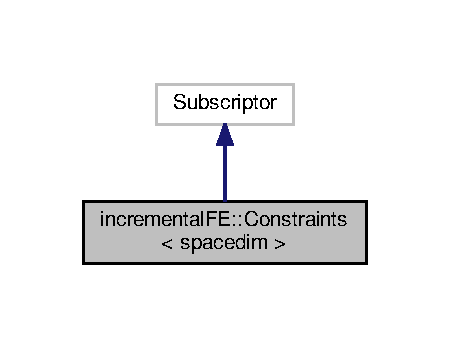
\includegraphics[width=229pt]{classincremental_f_e_1_1_constraints__inherit__graph}
\end{center}
\end{figure}


Collaboration diagram for incremental\+FE\+::Constraints$<$ spacedim $>$\+:\nopagebreak
\begin{figure}[H]
\begin{center}
\leavevmode
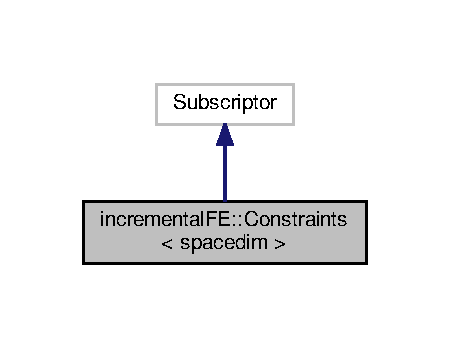
\includegraphics[width=229pt]{classincremental_f_e_1_1_constraints__coll__graph}
\end{center}
\end{figure}
\doxysubsection*{Public Member Functions}
\begin{DoxyCompactItemize}
\item 
\mbox{\hyperlink{classincremental_f_e_1_1_constraints_ab77495a668ae8925bd8095c2c80a8624}{$\sim$\+Constraints}} ()
\item 
void \mbox{\hyperlink{classincremental_f_e_1_1_constraints_a175a510cdecac4710d203eaf495b9af1}{add\+\_\+dirichlet\+\_\+constraint}} (const dealii\+::\+Galerkin\+Tools\+::\+Dirichlet\+Constraint$<$ spacedim $>$ \&dirichlet\+\_\+constraint, const double eval\+\_\+time=1.\+0)
\item 
void \mbox{\hyperlink{classincremental_f_e_1_1_constraints_a7cfbc9db3f165af1277b5652ca9e8a35}{add\+\_\+point\+\_\+constraint}} (const dealii\+::\+Galerkin\+Tools\+::\+Point\+Constraint$<$ spacedim, spacedim $>$ \&point\+\_\+constraint, const double eval\+\_\+time=1.\+0)
\item 
void \mbox{\hyperlink{classincremental_f_e_1_1_constraints_a1c76efebcd160d921d0b34d7ee11ec87}{add\+\_\+point\+\_\+constraint}} (const dealii\+::\+Galerkin\+Tools\+::\+Point\+Constraint$<$ spacedim-\/1, spacedim $>$ \&point\+\_\+constraint, const double eval\+\_\+time=1.\+0)
\item 
void \mbox{\hyperlink{classincremental_f_e_1_1_constraints_a24947a8db7f56ab508d5dacb263b162c}{add\+\_\+point\+\_\+constraint}} (const dealii\+::\+Galerkin\+Tools\+::\+Point\+Constraint$<$ 0, spacedim $>$ \&point\+\_\+constraint, const double eval\+\_\+time=1.\+0)
\item 
const std\+::vector$<$ const dealii\+::\+Galerkin\+Tools\+::\+Dirichlet\+Constraint$<$ spacedim $>$ $\ast$ $>$ \mbox{\hyperlink{classincremental_f_e_1_1_constraints_affbb56b906ba6cd817cf918bc9ff23c0}{get\+\_\+dirichlet\+\_\+constraints}} () const
\item 
const std\+::vector$<$ const dealii\+::\+Galerkin\+Tools\+::\+Point\+Constraint$<$ spacedim, spacedim $>$ $\ast$ $>$ \mbox{\hyperlink{classincremental_f_e_1_1_constraints_a0816d66cd0cd61581ccc56352a2019a1}{get\+\_\+point\+\_\+constraints\+\_\+domain}} () const
\item 
const std\+::vector$<$ const dealii\+::\+Galerkin\+Tools\+::\+Point\+Constraint$<$ spacedim-\/1, spacedim $>$ $\ast$ $>$ \mbox{\hyperlink{classincremental_f_e_1_1_constraints_af3f92a6860ae867ecc06ad129328c89b}{get\+\_\+point\+\_\+constraints\+\_\+interface}} () const
\item 
const std\+::vector$<$ const dealii\+::\+Galerkin\+Tools\+::\+Point\+Constraint$<$ 0, spacedim $>$ $\ast$ $>$ \mbox{\hyperlink{classincremental_f_e_1_1_constraints_ab24ae1229790edee6d5ab7146057f799}{get\+\_\+point\+\_\+constraints\+\_\+C}} () const
\item 
const std\+::set$<$ const dealii\+::\+Galerkin\+Tools\+::\+Independent\+Field$<$ 0, spacedim $>$ $\ast$ $>$ \mbox{\hyperlink{classincremental_f_e_1_1_constraints_af51722fecb3b4a84874bbaf9363b4ca3}{get\+\_\+independent\+\_\+scalars}} () const
\item 
void \mbox{\hyperlink{classincremental_f_e_1_1_constraints_aaced3150f751c28a801926e0e3675e10}{set\+\_\+time}} (const double begin\+\_\+time\+\_\+step, const double end\+\_\+time\+\_\+step) const
\end{DoxyCompactItemize}
\doxysubsection*{Private Attributes}
\begin{DoxyCompactItemize}
\item 
std\+::vector$<$ std\+::pair$<$ dealii\+::\+Smart\+Pointer$<$ const dealii\+::\+Galerkin\+Tools\+::\+Dirichlet\+Constraint$<$ spacedim $>$ $>$, double $>$ $>$ \mbox{\hyperlink{classincremental_f_e_1_1_constraints_a09c6e6159ef046baf2f460e42a8518f0}{dirichlet\+\_\+constraints}}
\item 
std\+::vector$<$ std\+::pair$<$ dealii\+::\+Smart\+Pointer$<$ const dealii\+::\+Galerkin\+Tools\+::\+Point\+Constraint$<$ spacedim, spacedim $>$ $>$, double $>$ $>$ \mbox{\hyperlink{classincremental_f_e_1_1_constraints_a4ae87574f87aec09d2d3014348ae1c7b}{point\+\_\+constraints\+\_\+domain}}
\item 
std\+::vector$<$ std\+::pair$<$ dealii\+::\+Smart\+Pointer$<$ const dealii\+::\+Galerkin\+Tools\+::\+Point\+Constraint$<$ spacedim-\/1, spacedim $>$ $>$, double $>$ $>$ \mbox{\hyperlink{classincremental_f_e_1_1_constraints_a4129a0bafb912ac39c1d3bc28bb2b9f5}{point\+\_\+constraints\+\_\+interface}}
\item 
std\+::vector$<$ std\+::pair$<$ dealii\+::\+Smart\+Pointer$<$ const dealii\+::\+Galerkin\+Tools\+::\+Point\+Constraint$<$ 0, spacedim $>$ $>$, double $>$ $>$ \mbox{\hyperlink{classincremental_f_e_1_1_constraints_a083dc1adfe8f79f0f16733dd6a13b5b3}{point\+\_\+constraints\+\_\+C}}
\end{DoxyCompactItemize}


\doxysubsection{Detailed Description}
\subsubsection*{template$<$unsigned int spacedim$>$\newline
class incremental\+F\+E\+::\+Constraints$<$ spacedim $>$}

Class collecting the constraints of the problem.

The \mbox{\hyperlink{classincremental_f_e_1_1_constraints}{Constraints}} class inherits from \textbf{ Subscriptor} in order to be able to check that \mbox{\hyperlink{classincremental_f_e_1_1_constraints}{Constraints}} objects are only destroyed when they are not needed anymore by other objects.


\begin{DoxyTemplParams}{Template Parameters}
{\em spacedim} & spatial dimension of the problem \\
\hline
\end{DoxyTemplParams}


\doxysubsection{Constructor \& Destructor Documentation}
\mbox{\Hypertarget{classincremental_f_e_1_1_constraints_ab77495a668ae8925bd8095c2c80a8624}\label{classincremental_f_e_1_1_constraints_ab77495a668ae8925bd8095c2c80a8624}} 
\index{incrementalFE::Constraints$<$ spacedim $>$@{incrementalFE::Constraints$<$ spacedim $>$}!````~Constraints@{$\sim$Constraints}}
\index{````~Constraints@{$\sim$Constraints}!incrementalFE::Constraints$<$ spacedim $>$@{incrementalFE::Constraints$<$ spacedim $>$}}
\doxysubsubsection{\texorpdfstring{$\sim$Constraints()}{~Constraints()}}
{\footnotesize\ttfamily template$<$unsigned int spacedim$>$ \\
\mbox{\hyperlink{classincremental_f_e_1_1_constraints}{incremental\+F\+E\+::\+Constraints}}$<$ spacedim $>$\+::$\sim$\mbox{\hyperlink{classincremental_f_e_1_1_constraints}{Constraints}} (\begin{DoxyParamCaption}{ }\end{DoxyParamCaption})}

The destructor of \mbox{\hyperlink{classincremental_f_e_1_1_constraints}{Constraints}} essentially checks before destruction that the \mbox{\hyperlink{classincremental_f_e_1_1_constraints}{Constraints}} object is not used by other objects. If this is the case, the program will be aborted. 

\doxysubsection{Member Function Documentation}
\mbox{\Hypertarget{classincremental_f_e_1_1_constraints_a175a510cdecac4710d203eaf495b9af1}\label{classincremental_f_e_1_1_constraints_a175a510cdecac4710d203eaf495b9af1}} 
\index{incrementalFE::Constraints$<$ spacedim $>$@{incrementalFE::Constraints$<$ spacedim $>$}!add\_dirichlet\_constraint@{add\_dirichlet\_constraint}}
\index{add\_dirichlet\_constraint@{add\_dirichlet\_constraint}!incrementalFE::Constraints$<$ spacedim $>$@{incrementalFE::Constraints$<$ spacedim $>$}}
\doxysubsubsection{\texorpdfstring{add\_dirichlet\_constraint()}{add\_dirichlet\_constraint()}}
{\footnotesize\ttfamily template$<$unsigned int spacedim$>$ \\
void \mbox{\hyperlink{classincremental_f_e_1_1_constraints}{incremental\+F\+E\+::\+Constraints}}$<$ spacedim $>$\+::add\+\_\+dirichlet\+\_\+constraint (\begin{DoxyParamCaption}\item[{const dealii\+::\+Galerkin\+Tools\+::\+Dirichlet\+Constraint$<$ spacedim $>$ \&}]{dirichlet\+\_\+constraint,  }\item[{const double}]{eval\+\_\+time = {\ttfamily 1.0} }\end{DoxyParamCaption})}

Add a \textbf{ Dirichlet\+Constraint} to \mbox{\hyperlink{classincremental_f_e_1_1_constraints_a09c6e6159ef046baf2f460e42a8518f0}{Constraints\+::dirichlet\+\_\+constraints}}


\begin{DoxyParams}[1]{Parameters}
\mbox{\texttt{ in}}  & {\em dirichlet\+\_\+constraint} & \textbf{ Dirichlet\+Constraint} object\\
\hline
\mbox{\texttt{ in}}  & {\em eval\+\_\+time} & Evaluation time of constraint, see Constraints\+::dirichlet\+\_\+constraints\+\_\+domain\+\_\+eval\+\_\+time \\
\hline
\end{DoxyParams}
\mbox{\Hypertarget{classincremental_f_e_1_1_constraints_a24947a8db7f56ab508d5dacb263b162c}\label{classincremental_f_e_1_1_constraints_a24947a8db7f56ab508d5dacb263b162c}} 
\index{incrementalFE::Constraints$<$ spacedim $>$@{incrementalFE::Constraints$<$ spacedim $>$}!add\_point\_constraint@{add\_point\_constraint}}
\index{add\_point\_constraint@{add\_point\_constraint}!incrementalFE::Constraints$<$ spacedim $>$@{incrementalFE::Constraints$<$ spacedim $>$}}
\doxysubsubsection{\texorpdfstring{add\_point\_constraint()}{add\_point\_constraint()}\hspace{0.1cm}{\footnotesize\ttfamily [1/3]}}
{\footnotesize\ttfamily template$<$unsigned int spacedim$>$ \\
void \mbox{\hyperlink{classincremental_f_e_1_1_constraints}{incremental\+F\+E\+::\+Constraints}}$<$ spacedim $>$\+::add\+\_\+point\+\_\+constraint (\begin{DoxyParamCaption}\item[{const dealii\+::\+Galerkin\+Tools\+::\+Point\+Constraint$<$ 0, spacedim $>$ \&}]{point\+\_\+constraint,  }\item[{const double}]{eval\+\_\+time = {\ttfamily 1.0} }\end{DoxyParamCaption})}

Add an independent scalar related Point\+Constraint to \mbox{\hyperlink{classincremental_f_e_1_1_constraints_a083dc1adfe8f79f0f16733dd6a13b5b3}{Constraints\+::point\+\_\+constraints\+\_\+C}}


\begin{DoxyParams}[1]{Parameters}
\mbox{\texttt{ in}}  & {\em point\+\_\+constraint} & Point\+Constraint object\\
\hline
\mbox{\texttt{ in}}  & {\em eval\+\_\+time} & Evaluation time of constraint, see Constraints\+::point\+\_\+constraints\+\_\+\+C\+\_\+eval\+\_\+time \\
\hline
\end{DoxyParams}
\mbox{\Hypertarget{classincremental_f_e_1_1_constraints_a7cfbc9db3f165af1277b5652ca9e8a35}\label{classincremental_f_e_1_1_constraints_a7cfbc9db3f165af1277b5652ca9e8a35}} 
\index{incrementalFE::Constraints$<$ spacedim $>$@{incrementalFE::Constraints$<$ spacedim $>$}!add\_point\_constraint@{add\_point\_constraint}}
\index{add\_point\_constraint@{add\_point\_constraint}!incrementalFE::Constraints$<$ spacedim $>$@{incrementalFE::Constraints$<$ spacedim $>$}}
\doxysubsubsection{\texorpdfstring{add\_point\_constraint()}{add\_point\_constraint()}\hspace{0.1cm}{\footnotesize\ttfamily [2/3]}}
{\footnotesize\ttfamily template$<$unsigned int spacedim$>$ \\
void \mbox{\hyperlink{classincremental_f_e_1_1_constraints}{incremental\+F\+E\+::\+Constraints}}$<$ spacedim $>$\+::add\+\_\+point\+\_\+constraint (\begin{DoxyParamCaption}\item[{const dealii\+::\+Galerkin\+Tools\+::\+Point\+Constraint$<$ spacedim, spacedim $>$ \&}]{point\+\_\+constraint,  }\item[{const double}]{eval\+\_\+time = {\ttfamily 1.0} }\end{DoxyParamCaption})}

Add a domain-\/related Point\+Constraint to \mbox{\hyperlink{classincremental_f_e_1_1_constraints_a4ae87574f87aec09d2d3014348ae1c7b}{Constraints\+::point\+\_\+constraints\+\_\+domain}}


\begin{DoxyParams}[1]{Parameters}
\mbox{\texttt{ in}}  & {\em point\+\_\+constraint} & Point\+Constraint object\\
\hline
\mbox{\texttt{ in}}  & {\em eval\+\_\+time} & Evaluation time of constraint, see Constraints\+::point\+\_\+constraints\+\_\+domain\+\_\+eval\+\_\+time \\
\hline
\end{DoxyParams}
\mbox{\Hypertarget{classincremental_f_e_1_1_constraints_a1c76efebcd160d921d0b34d7ee11ec87}\label{classincremental_f_e_1_1_constraints_a1c76efebcd160d921d0b34d7ee11ec87}} 
\index{incrementalFE::Constraints$<$ spacedim $>$@{incrementalFE::Constraints$<$ spacedim $>$}!add\_point\_constraint@{add\_point\_constraint}}
\index{add\_point\_constraint@{add\_point\_constraint}!incrementalFE::Constraints$<$ spacedim $>$@{incrementalFE::Constraints$<$ spacedim $>$}}
\doxysubsubsection{\texorpdfstring{add\_point\_constraint()}{add\_point\_constraint()}\hspace{0.1cm}{\footnotesize\ttfamily [3/3]}}
{\footnotesize\ttfamily template$<$unsigned int spacedim$>$ \\
void \mbox{\hyperlink{classincremental_f_e_1_1_constraints}{incremental\+F\+E\+::\+Constraints}}$<$ spacedim $>$\+::add\+\_\+point\+\_\+constraint (\begin{DoxyParamCaption}\item[{const dealii\+::\+Galerkin\+Tools\+::\+Point\+Constraint$<$ spacedim-\/1, spacedim $>$ \&}]{point\+\_\+constraint,  }\item[{const double}]{eval\+\_\+time = {\ttfamily 1.0} }\end{DoxyParamCaption})}

Add an interface-\/related Point\+Constraint to \mbox{\hyperlink{classincremental_f_e_1_1_constraints_a4129a0bafb912ac39c1d3bc28bb2b9f5}{Constraints\+::point\+\_\+constraints\+\_\+interface}}


\begin{DoxyParams}[1]{Parameters}
\mbox{\texttt{ in}}  & {\em point\+\_\+constraint} & Point\+Constraint object\\
\hline
\mbox{\texttt{ in}}  & {\em eval\+\_\+time} & Evaluation time of constraint, see Constraints\+::point\+\_\+constraints\+\_\+interface\+\_\+eval\+\_\+time \\
\hline
\end{DoxyParams}
\mbox{\Hypertarget{classincremental_f_e_1_1_constraints_affbb56b906ba6cd817cf918bc9ff23c0}\label{classincremental_f_e_1_1_constraints_affbb56b906ba6cd817cf918bc9ff23c0}} 
\index{incrementalFE::Constraints$<$ spacedim $>$@{incrementalFE::Constraints$<$ spacedim $>$}!get\_dirichlet\_constraints@{get\_dirichlet\_constraints}}
\index{get\_dirichlet\_constraints@{get\_dirichlet\_constraints}!incrementalFE::Constraints$<$ spacedim $>$@{incrementalFE::Constraints$<$ spacedim $>$}}
\doxysubsubsection{\texorpdfstring{get\_dirichlet\_constraints()}{get\_dirichlet\_constraints()}}
{\footnotesize\ttfamily template$<$unsigned int spacedim$>$ \\
const std\+::vector$<$ const dealii\+::\+Galerkin\+Tools\+::\+Dirichlet\+Constraint$<$spacedim$>$$\ast$ $>$ \mbox{\hyperlink{classincremental_f_e_1_1_constraints}{incremental\+F\+E\+::\+Constraints}}$<$ spacedim $>$\+::get\+\_\+dirichlet\+\_\+constraints (\begin{DoxyParamCaption}{ }\end{DoxyParamCaption}) const}

\begin{DoxyReturn}{Returns}
A vector with pointers to the \textbf{ Dirichlet\+Constraint} objects in \mbox{\hyperlink{classincremental_f_e_1_1_constraints_a09c6e6159ef046baf2f460e42a8518f0}{Constraints\+::dirichlet\+\_\+constraints}} 
\end{DoxyReturn}
\mbox{\Hypertarget{classincremental_f_e_1_1_constraints_af51722fecb3b4a84874bbaf9363b4ca3}\label{classincremental_f_e_1_1_constraints_af51722fecb3b4a84874bbaf9363b4ca3}} 
\index{incrementalFE::Constraints$<$ spacedim $>$@{incrementalFE::Constraints$<$ spacedim $>$}!get\_independent\_scalars@{get\_independent\_scalars}}
\index{get\_independent\_scalars@{get\_independent\_scalars}!incrementalFE::Constraints$<$ spacedim $>$@{incrementalFE::Constraints$<$ spacedim $>$}}
\doxysubsubsection{\texorpdfstring{get\_independent\_scalars()}{get\_independent\_scalars()}}
{\footnotesize\ttfamily template$<$unsigned int spacedim$>$ \\
const std\+::set$<$ const dealii\+::\+Galerkin\+Tools\+::\+Independent\+Field$<$0, spacedim$>$$\ast$ $>$ \mbox{\hyperlink{classincremental_f_e_1_1_constraints}{incremental\+F\+E\+::\+Constraints}}$<$ spacedim $>$\+::get\+\_\+independent\+\_\+scalars (\begin{DoxyParamCaption}{ }\end{DoxyParamCaption}) const}

\begin{DoxyReturn}{Returns}
The independent scalars involved in the definition of the constraints. 
\end{DoxyReturn}
\mbox{\Hypertarget{classincremental_f_e_1_1_constraints_ab24ae1229790edee6d5ab7146057f799}\label{classincremental_f_e_1_1_constraints_ab24ae1229790edee6d5ab7146057f799}} 
\index{incrementalFE::Constraints$<$ spacedim $>$@{incrementalFE::Constraints$<$ spacedim $>$}!get\_point\_constraints\_C@{get\_point\_constraints\_C}}
\index{get\_point\_constraints\_C@{get\_point\_constraints\_C}!incrementalFE::Constraints$<$ spacedim $>$@{incrementalFE::Constraints$<$ spacedim $>$}}
\doxysubsubsection{\texorpdfstring{get\_point\_constraints\_C()}{get\_point\_constraints\_C()}}
{\footnotesize\ttfamily template$<$unsigned int spacedim$>$ \\
const std\+::vector$<$ const dealii\+::\+Galerkin\+Tools\+::\+Point\+Constraint$<$0, spacedim$>$$\ast$ $>$ \mbox{\hyperlink{classincremental_f_e_1_1_constraints}{incremental\+F\+E\+::\+Constraints}}$<$ spacedim $>$\+::get\+\_\+point\+\_\+constraints\+\_\+C (\begin{DoxyParamCaption}{ }\end{DoxyParamCaption}) const}

\begin{DoxyReturn}{Returns}
A vector with pointers to the independent scalar related constraint objects in \mbox{\hyperlink{classincremental_f_e_1_1_constraints_a083dc1adfe8f79f0f16733dd6a13b5b3}{Constraints\+::point\+\_\+constraints\+\_\+C}} 
\end{DoxyReturn}
\mbox{\Hypertarget{classincremental_f_e_1_1_constraints_a0816d66cd0cd61581ccc56352a2019a1}\label{classincremental_f_e_1_1_constraints_a0816d66cd0cd61581ccc56352a2019a1}} 
\index{incrementalFE::Constraints$<$ spacedim $>$@{incrementalFE::Constraints$<$ spacedim $>$}!get\_point\_constraints\_domain@{get\_point\_constraints\_domain}}
\index{get\_point\_constraints\_domain@{get\_point\_constraints\_domain}!incrementalFE::Constraints$<$ spacedim $>$@{incrementalFE::Constraints$<$ spacedim $>$}}
\doxysubsubsection{\texorpdfstring{get\_point\_constraints\_domain()}{get\_point\_constraints\_domain()}}
{\footnotesize\ttfamily template$<$unsigned int spacedim$>$ \\
const std\+::vector$<$ const dealii\+::\+Galerkin\+Tools\+::\+Point\+Constraint$<$spacedim, spacedim$>$$\ast$ $>$ \mbox{\hyperlink{classincremental_f_e_1_1_constraints}{incremental\+F\+E\+::\+Constraints}}$<$ spacedim $>$\+::get\+\_\+point\+\_\+constraints\+\_\+domain (\begin{DoxyParamCaption}{ }\end{DoxyParamCaption}) const}

\begin{DoxyReturn}{Returns}
A vector with pointers to the domain related constraint objects in \mbox{\hyperlink{classincremental_f_e_1_1_constraints_a4ae87574f87aec09d2d3014348ae1c7b}{Constraints\+::point\+\_\+constraints\+\_\+domain}} 
\end{DoxyReturn}
\mbox{\Hypertarget{classincremental_f_e_1_1_constraints_af3f92a6860ae867ecc06ad129328c89b}\label{classincremental_f_e_1_1_constraints_af3f92a6860ae867ecc06ad129328c89b}} 
\index{incrementalFE::Constraints$<$ spacedim $>$@{incrementalFE::Constraints$<$ spacedim $>$}!get\_point\_constraints\_interface@{get\_point\_constraints\_interface}}
\index{get\_point\_constraints\_interface@{get\_point\_constraints\_interface}!incrementalFE::Constraints$<$ spacedim $>$@{incrementalFE::Constraints$<$ spacedim $>$}}
\doxysubsubsection{\texorpdfstring{get\_point\_constraints\_interface()}{get\_point\_constraints\_interface()}}
{\footnotesize\ttfamily template$<$unsigned int spacedim$>$ \\
const std\+::vector$<$ const dealii\+::\+Galerkin\+Tools\+::\+Point\+Constraint$<$spacedim-\/1, spacedim$>$$\ast$ $>$ \mbox{\hyperlink{classincremental_f_e_1_1_constraints}{incremental\+F\+E\+::\+Constraints}}$<$ spacedim $>$\+::get\+\_\+point\+\_\+constraints\+\_\+interface (\begin{DoxyParamCaption}{ }\end{DoxyParamCaption}) const}

\begin{DoxyReturn}{Returns}
A vector with pointers to the interface related constraint objects in \mbox{\hyperlink{classincremental_f_e_1_1_constraints_a4129a0bafb912ac39c1d3bc28bb2b9f5}{Constraints\+::point\+\_\+constraints\+\_\+interface}} 
\end{DoxyReturn}
\mbox{\Hypertarget{classincremental_f_e_1_1_constraints_aaced3150f751c28a801926e0e3675e10}\label{classincremental_f_e_1_1_constraints_aaced3150f751c28a801926e0e3675e10}} 
\index{incrementalFE::Constraints$<$ spacedim $>$@{incrementalFE::Constraints$<$ spacedim $>$}!set\_time@{set\_time}}
\index{set\_time@{set\_time}!incrementalFE::Constraints$<$ spacedim $>$@{incrementalFE::Constraints$<$ spacedim $>$}}
\doxysubsubsection{\texorpdfstring{set\_time()}{set\_time()}}
{\footnotesize\ttfamily template$<$unsigned int spacedim$>$ \\
void \mbox{\hyperlink{classincremental_f_e_1_1_constraints}{incremental\+F\+E\+::\+Constraints}}$<$ spacedim $>$\+::set\+\_\+time (\begin{DoxyParamCaption}\item[{const double}]{begin\+\_\+time\+\_\+step,  }\item[{const double}]{end\+\_\+time\+\_\+step }\end{DoxyParamCaption}) const}

Update the evaluation time of the constraints for the upcoming time-\/step


\begin{DoxyParams}[1]{Parameters}
\mbox{\texttt{ in}}  & {\em begin\+\_\+time\+\_\+step} & Time at the start of the time step\\
\hline
\mbox{\texttt{ in}}  & {\em end\+\_\+time\+\_\+step} & Time at the end of the time step \\
\hline
\end{DoxyParams}


\doxysubsection{Member Data Documentation}
\mbox{\Hypertarget{classincremental_f_e_1_1_constraints_a09c6e6159ef046baf2f460e42a8518f0}\label{classincremental_f_e_1_1_constraints_a09c6e6159ef046baf2f460e42a8518f0}} 
\index{incrementalFE::Constraints$<$ spacedim $>$@{incrementalFE::Constraints$<$ spacedim $>$}!dirichlet\_constraints@{dirichlet\_constraints}}
\index{dirichlet\_constraints@{dirichlet\_constraints}!incrementalFE::Constraints$<$ spacedim $>$@{incrementalFE::Constraints$<$ spacedim $>$}}
\doxysubsubsection{\texorpdfstring{dirichlet\_constraints}{dirichlet\_constraints}}
{\footnotesize\ttfamily template$<$unsigned int spacedim$>$ \\
std\+::vector$<$ std\+::pair$<$dealii\+::\+Smart\+Pointer$<$const dealii\+::\+Galerkin\+Tools\+::\+Dirichlet\+Constraint$<$spacedim$>$ $>$, double$>$ $>$ \mbox{\hyperlink{classincremental_f_e_1_1_constraints}{incremental\+F\+E\+::\+Constraints}}$<$ spacedim $>$\+::dirichlet\+\_\+constraints\hspace{0.3cm}{\ttfamily [private]}}

Vector with the \textbf{ Dirichlet\+Constraint} objects

The first element of each pair is the constraint.

The second entry of each pair defines the instant of time within a time step, at which the time dependent functions of the corresponding constraint (e.\+g. the constraint inhomogeneities) are evaluated. In particular, values in the range \mbox{[}0, 1\mbox{]} are admissible for each entry, where e.\+g. 0 means that the time dependent functions are evaluated at the time corresponding to the beginning of the time step and 1 means that they are evaluated at the time corresponding to the end of the time step.

Typically, the constraints for state and process variables are evaluated at the end of the time step, while constraints for Lagrangian multipliers are evaluated at the instant of time corresponding to the time integration parameter $\alpha$. \mbox{\Hypertarget{classincremental_f_e_1_1_constraints_a083dc1adfe8f79f0f16733dd6a13b5b3}\label{classincremental_f_e_1_1_constraints_a083dc1adfe8f79f0f16733dd6a13b5b3}} 
\index{incrementalFE::Constraints$<$ spacedim $>$@{incrementalFE::Constraints$<$ spacedim $>$}!point\_constraints\_C@{point\_constraints\_C}}
\index{point\_constraints\_C@{point\_constraints\_C}!incrementalFE::Constraints$<$ spacedim $>$@{incrementalFE::Constraints$<$ spacedim $>$}}
\doxysubsubsection{\texorpdfstring{point\_constraints\_C}{point\_constraints\_C}}
{\footnotesize\ttfamily template$<$unsigned int spacedim$>$ \\
std\+::vector$<$ std\+::pair$<$dealii\+::\+Smart\+Pointer$<$const dealii\+::\+Galerkin\+Tools\+::\+Point\+Constraint$<$0, spacedim$>$ $>$, double$>$ $>$ \mbox{\hyperlink{classincremental_f_e_1_1_constraints}{incremental\+F\+E\+::\+Constraints}}$<$ spacedim $>$\+::point\+\_\+constraints\+\_\+C\hspace{0.3cm}{\ttfamily [private]}}

Vector with independent scalar related constraints

The first element of each pair is the constraint.

The second entry of each pair defines the instant of time within a time step, at which the time dependent functions of the corresponding constraint (e.\+g. the constraint inhomogeneities) are evaluated. In particular, values in the range \mbox{[}0, 1\mbox{]} are admissible for each entry, where e.\+g. 0 means that the time dependent functions are evaluated at the time corresponding to the beginning of the time step and 1 means that they are evaluated at the time corresponding to the end of the time step.

Typically, the constraints for state and process variables are evaluated at the end of the time step, while constraints for Lagrangian multipliers are evaluated at the instant of time corresponding to the time integration parameter $\alpha$. \mbox{\Hypertarget{classincremental_f_e_1_1_constraints_a4ae87574f87aec09d2d3014348ae1c7b}\label{classincremental_f_e_1_1_constraints_a4ae87574f87aec09d2d3014348ae1c7b}} 
\index{incrementalFE::Constraints$<$ spacedim $>$@{incrementalFE::Constraints$<$ spacedim $>$}!point\_constraints\_domain@{point\_constraints\_domain}}
\index{point\_constraints\_domain@{point\_constraints\_domain}!incrementalFE::Constraints$<$ spacedim $>$@{incrementalFE::Constraints$<$ spacedim $>$}}
\doxysubsubsection{\texorpdfstring{point\_constraints\_domain}{point\_constraints\_domain}}
{\footnotesize\ttfamily template$<$unsigned int spacedim$>$ \\
std\+::vector$<$ std\+::pair$<$dealii\+::\+Smart\+Pointer$<$const dealii\+::\+Galerkin\+Tools\+::\+Point\+Constraint$<$spacedim, spacedim$>$ $>$, double$>$ $>$ \mbox{\hyperlink{classincremental_f_e_1_1_constraints}{incremental\+F\+E\+::\+Constraints}}$<$ spacedim $>$\+::point\+\_\+constraints\+\_\+domain\hspace{0.3cm}{\ttfamily [private]}}

Vector with domain related point constraints

The first element of each pair is the constraint.

The second entry of each pair defines the instant of time within a time step, at which the time dependent functions of the corresponding constraint (e.\+g. the constraint inhomogeneities) are evaluated. In particular, values in the range \mbox{[}0, 1\mbox{]} are admissible for each entry, where e.\+g. 0 means that the time dependent functions are evaluated at the time corresponding to the beginning of the time step and 1 means that they are evaluated at the time corresponding to the end of the time step.

Typically, the constraints for state and process variables are evaluated at the end of the time step, while constraints for Lagrangian multipliers are evaluated at the instant of time corresponding to the time integration parameter $\alpha$. \mbox{\Hypertarget{classincremental_f_e_1_1_constraints_a4129a0bafb912ac39c1d3bc28bb2b9f5}\label{classincremental_f_e_1_1_constraints_a4129a0bafb912ac39c1d3bc28bb2b9f5}} 
\index{incrementalFE::Constraints$<$ spacedim $>$@{incrementalFE::Constraints$<$ spacedim $>$}!point\_constraints\_interface@{point\_constraints\_interface}}
\index{point\_constraints\_interface@{point\_constraints\_interface}!incrementalFE::Constraints$<$ spacedim $>$@{incrementalFE::Constraints$<$ spacedim $>$}}
\doxysubsubsection{\texorpdfstring{point\_constraints\_interface}{point\_constraints\_interface}}
{\footnotesize\ttfamily template$<$unsigned int spacedim$>$ \\
std\+::vector$<$ std\+::pair$<$dealii\+::\+Smart\+Pointer$<$const dealii\+::\+Galerkin\+Tools\+::\+Point\+Constraint$<$spacedim-\/1, spacedim$>$ $>$, double$>$ $>$ \mbox{\hyperlink{classincremental_f_e_1_1_constraints}{incremental\+F\+E\+::\+Constraints}}$<$ spacedim $>$\+::point\+\_\+constraints\+\_\+interface\hspace{0.3cm}{\ttfamily [private]}}

Vector with interface related point constraints

The first element of each pair is the constraint.

The second entry of each pair defines the instant of time within a time step, at which the time dependent functions of the corresponding constraint (e.\+g. the constraint inhomogeneities) are evaluated. In particular, values in the range \mbox{[}0, 1\mbox{]} are admissible for each entry, where e.\+g. 0 means that the time dependent functions are evaluated at the time corresponding to the beginning of the time step and 1 means that they are evaluated at the time corresponding to the end of the time step.

Typically, the constraints for state and process variables are evaluated at the end of the time step, while constraints for Lagrangian multipliers are evaluated at the instant of time corresponding to the time integration parameter $\alpha$. 

The documentation for this class was generated from the following file\+:\begin{DoxyCompactItemize}
\item 
/home/sst/code/\+Incremental\+F\+E/\+Incremental\+F\+E/include/incremental\+\_\+fe/\mbox{\hyperlink{constraints_8h}{constraints.\+h}}\end{DoxyCompactItemize}

\hypertarget{classincremental_f_e_1_1_f_e_model}{}\doxysection{incremental\+FE\+::F\+E\+Model$<$ spacedim, Solution\+Vector\+Type, R\+H\+S\+Vector\+Type, Matrix\+Type $>$ Class Template Reference}
\label{classincremental_f_e_1_1_f_e_model}\index{incrementalFE::FEModel$<$ spacedim, SolutionVectorType, RHSVectorType, MatrixType $>$@{incrementalFE::FEModel$<$ spacedim, SolutionVectorType, RHSVectorType, MatrixType $>$}}


{\ttfamily \#include $<$fe\+\_\+model.\+h$>$}

\doxysubsection*{Public Member Functions}
\begin{DoxyCompactItemize}
\item 
\mbox{\hyperlink{classincremental_f_e_1_1_f_e_model_a3a85e9c068ca9ba6959b2aa3dc25812d}{F\+E\+Model}} (const dealii\+::\+Galerkin\+Tools\+::\+Total\+Potential$<$ spacedim $>$ \&total\+\_\+potential, dealii\+::\+Galerkin\+Tools\+::\+Triangulation\+System$<$ spacedim $>$ \&tria\+\_\+system, const dealii\+::\+Mapping$<$ spacedim, spacedim $>$ \&mapping\+\_\+domain, const dealii\+::\+Mapping$<$ spacedim-\/1, spacedim $>$ \&mapping\+\_\+interface, \mbox{\hyperlink{classincremental_f_e_1_1_global_data_incremental_f_e}{Global\+Data\+Incremental\+FE}}$<$ spacedim $>$ \&\mbox{\hyperlink{classincremental_f_e_1_1_f_e_model_aa6f80778241b26906af1f571517102dd}{global\+\_\+data}}, const \mbox{\hyperlink{classincremental_f_e_1_1_constraints}{Constraints}}$<$ spacedim $>$ \&\mbox{\hyperlink{classincremental_f_e_1_1_f_e_model_a33a622c3c53ea4bee3bdefac06201c70}{constraints}}, dealii\+::\+Galerkin\+Tools\+::\+Solver\+Wrapper$<$ Solution\+Vector\+Type, R\+H\+S\+Vector\+Type, Matrix\+Type, dealii\+::\+Galerkin\+Tools\+::\+Two\+Block\+Sparsity\+Pattern $>$ \&\mbox{\hyperlink{classincremental_f_e_1_1_f_e_model_ad53a49fc1326472b11e3e3273b5f6f7b}{solver\+\_\+wrapper}}, const bool \mbox{\hyperlink{classincremental_f_e_1_1_f_e_model_a65b5910cfba2feb26933ad451ceff628}{make\+\_\+hanging\+\_\+node\+\_\+constraints}}=true, const bool \mbox{\hyperlink{classincremental_f_e_1_1_f_e_model_ace70f6d085e2b37c0241f9eb0ca5d178}{single\+\_\+block}}=false)
\item 
\mbox{\hyperlink{classincremental_f_e_1_1_f_e_model_ae4d9513474928ef225245928410f984b}{$\sim$\+F\+E\+Model}} ()
\item 
int \mbox{\hyperlink{classincremental_f_e_1_1_f_e_model_a1528bdeba89d6f4774526a2ed9412047}{do\+\_\+time\+\_\+step}} (const double t, const dealii\+::\+Affine\+Constraints$<$ double $>$ \&custom\+\_\+constraints=dealii\+::\+Affine\+Constraints$<$ double $>$(), const dealii\+::\+Affine\+Constraints$<$ double $>$ \&ignore\+\_\+constraints=dealii\+::\+Affine\+Constraints$<$ double $>$())
\item 
std\+::pair$<$ const double, const double $>$ \mbox{\hyperlink{classincremental_f_e_1_1_f_e_model_a9a5e7dc18c6acecde5265ff9f39e40ed}{compute\+\_\+distance\+\_\+to\+\_\+other\+\_\+solution}} (const \mbox{\hyperlink{classincremental_f_e_1_1_f_e_model}{F\+E\+Model}}$<$ spacedim, Solution\+Vector\+Type, R\+H\+S\+Vector\+Type, Matrix\+Type $>$ \&other\+\_\+incremental\+\_\+fe, const dealii\+::\+Quadrature$<$ spacedim $>$ quadrature\+\_\+domain, const dealii\+::\+Quadrature$<$ spacedim-\/1 $>$ quadrature\+\_\+interface, const \textbf{ dealii\+::\+Vector\+Tools\+::\+Norm\+Type} norm\+\_\+type=dealii\+::\+Vector\+Tools\+::\+Norm\+Type\+::\+L2\+\_\+norm, const dealii\+::\+Component\+Mask component\+\_\+mask\+\_\+domain=dealii\+::\+Component\+Mask(), const dealii\+::\+Component\+Mask component\+\_\+mask\+\_\+interface=dealii\+::\+Component\+Mask(), const double exponent=2.\+0, const \textbf{ dealii\+::\+Vector}$<$ double $>$ scaling\+\_\+domain=\textbf{ dealii\+::\+Vector}$<$ double $>$(), const \textbf{ dealii\+::\+Vector}$<$ double $>$ scaling\+\_\+interface=\textbf{ dealii\+::\+Vector}$<$ double $>$()) const
\item 
std\+::pair$<$ const double, const double $>$ \mbox{\hyperlink{classincremental_f_e_1_1_f_e_model_a0dd4646e08210f326f304814808e92e0}{compute\+\_\+distance\+\_\+to\+\_\+exact\+\_\+solution}} (const dealii\+::\+Function$<$ spacedim $>$ \&exact\+\_\+solution\+\_\+domain, const dealii\+::\+Function$<$ spacedim $>$ \&exact\+\_\+solution\+\_\+interface, const dealii\+::\+Quadrature$<$ spacedim $>$ quadrature\+\_\+domain, const dealii\+::\+Quadrature$<$ spacedim-\/1 $>$ quadrature\+\_\+interface, const \textbf{ dealii\+::\+Vector\+Tools\+::\+Norm\+Type} norm\+\_\+type=dealii\+::\+Vector\+Tools\+::\+Norm\+Type\+::\+L2\+\_\+norm, const dealii\+::\+Component\+Mask component\+\_\+mask\+\_\+domain=dealii\+::\+Component\+Mask(), const dealii\+::\+Component\+Mask component\+\_\+mask\+\_\+interface=dealii\+::\+Component\+Mask(), const double exponent=2.\+0) const
\item 
void \mbox{\hyperlink{classincremental_f_e_1_1_f_e_model_acb0d11f9d7a71971732d041a5cb4376a}{read\+\_\+solution\+\_\+from\+\_\+file}} (const std\+::string file\+\_\+name)
\item 
void \mbox{\hyperlink{classincremental_f_e_1_1_f_e_model_ac358550b1f5b47486199bcc870621d4f}{write\+\_\+solution\+\_\+to\+\_\+file}} (const std\+::string file\+\_\+name) const
\item 
void \mbox{\hyperlink{classincremental_f_e_1_1_f_e_model_a2e13285d3ec061e14dacaaf174ee5bf5}{write\+\_\+output\+\_\+independent\+\_\+fields}} (const std\+::string file\+\_\+name\+\_\+domain, const std\+::string file\+\_\+name\+\_\+interface, const unsigned int n\+\_\+subdivisions=1)
\item 
dealii\+::\+Galerkin\+Tools\+::\+Assembly\+Helper$<$ spacedim $>$ \& \mbox{\hyperlink{classincremental_f_e_1_1_f_e_model_aa3df4f846cc765c10e7c939353c845c6}{get\+\_\+assembly\+\_\+helper}} ()
\item 
double \mbox{\hyperlink{classincremental_f_e_1_1_f_e_model_aef592e091e60e8b3f99f601a59a68da6}{get\+\_\+potential\+\_\+value}} () const
\item 
void \mbox{\hyperlink{classincremental_f_e_1_1_f_e_model_af838cd26f882b0a70ece37a0199a0384}{attach\+\_\+data\+\_\+postprocessor\+\_\+domain}} (const dealii\+::\+Data\+Postprocessor$<$ spacedim $>$ \&dp)
\item 
void \mbox{\hyperlink{classincremental_f_e_1_1_f_e_model_a021c3223c447ac210a9c994abeaa7495}{attach\+\_\+data\+\_\+postprocessor\+\_\+interface}} (const dealii\+::\+Data\+Postprocessor$<$ spacedim $>$ \&dp)
\item 
const Solution\+Vector\+Type \& \mbox{\hyperlink{classincremental_f_e_1_1_f_e_model_ac23429ff2ae2b7c3cebb926626c70e45}{get\+\_\+solution\+\_\+vector}} () const
\item 
Solution\+Vector\+Type \& \mbox{\hyperlink{classincremental_f_e_1_1_f_e_model_a9a67ea7fc307135548010b550414199c}{get\+\_\+solution\+\_\+vector}} ()
\item 
const Solution\+Vector\+Type \& \mbox{\hyperlink{classincremental_f_e_1_1_f_e_model_a43bb2f22537dcec62961fc59f450584c}{get\+\_\+solution\+\_\+ref\+\_\+vector}} () const
\item 
Solution\+Vector\+Type \& \mbox{\hyperlink{classincremental_f_e_1_1_f_e_model_abbaf168f99be661e22d82ea1dd59d8ae}{get\+\_\+solution\+\_\+ref\+\_\+vector}} ()
\item 
Matrix\+Type \& \mbox{\hyperlink{classincremental_f_e_1_1_f_e_model_a2f5c0e7ac2d043a5c19fcc32927a76ce}{get\+\_\+system\+\_\+matrix}} ()
\item 
R\+H\+S\+Vector\+Type \& \mbox{\hyperlink{classincremental_f_e_1_1_f_e_model_a2940e902f0f30ae4b9b122f7c573a20d}{get\+\_\+rhs}} ()
\item 
double \mbox{\hyperlink{classincremental_f_e_1_1_f_e_model_a9cd396b8078926ba01eafe296152917b}{get\+\_\+solve\+\_\+time\+\_\+last\+\_\+step}} () const
\end{DoxyCompactItemize}
\doxysubsection*{Public Attributes}
\begin{DoxyCompactItemize}
\item 
boost\+::signals2\+::signal$<$ void()$>$ \mbox{\hyperlink{classincremental_f_e_1_1_f_e_model_a0992ed47497719c04caa8cbd5289a17b}{pre\+\_\+assembly}}
\item 
boost\+::signals2\+::signal$<$ void()$>$ \mbox{\hyperlink{classincremental_f_e_1_1_f_e_model_ac5c2edc96caa3b5ca1e55a655c56873e}{post\+\_\+assembly}}
\end{DoxyCompactItemize}
\doxysubsection*{Private Member Functions}
\begin{DoxyCompactItemize}
\item 
void \mbox{\hyperlink{classincremental_f_e_1_1_f_e_model_ae792df01f91eab7c12ecf41b7e8c514b}{reinit\+\_\+solution\+\_\+vector}} (Solution\+Vector\+Type \&vector)
\item 
void \mbox{\hyperlink{classincremental_f_e_1_1_f_e_model_aa8f0eaa319c21a88310d813fb34213f6}{reinit\+\_\+rhs\+\_\+vector}} (R\+H\+S\+Vector\+Type \&vector)
\item 
void \mbox{\hyperlink{classincremental_f_e_1_1_f_e_model_aca9a1d1eb2233b6dbfac86e14a092729}{reinit\+\_\+matrix}} (Matrix\+Type \&matrix)
\item 
bool \mbox{\hyperlink{classincremental_f_e_1_1_f_e_model_aa787a163ccf91fc13f2f5fb32d069253}{compute\+\_\+system}} (const Solution\+Vector\+Type \&\mbox{\hyperlink{classincremental_f_e_1_1_f_e_model_ad5f39fec8540d81155770764f945f572}{solution\+\_\+ref}}, dealii\+::\+Affine\+Constraints$<$ double $>$ \&\mbox{\hyperlink{classincremental_f_e_1_1_f_e_model_a33a622c3c53ea4bee3bdefac06201c70}{constraints}}, const bool first\+\_\+assembly=false)
\item 
void \mbox{\hyperlink{classincremental_f_e_1_1_f_e_model_a7c5c84e081ebe20e373ec5d2abc359b7}{compute\+\_\+sparsity\+\_\+pattern}} (const dealii\+::\+Affine\+Constraints$<$ double $>$ \&\mbox{\hyperlink{classincremental_f_e_1_1_f_e_model_a33a622c3c53ea4bee3bdefac06201c70}{constraints}})
\item 
void \mbox{\hyperlink{classincremental_f_e_1_1_f_e_model_ae96fd0a7b6688ed844059d2636e923cc}{make\+\_\+constraints}} (dealii\+::\+Affine\+Constraints$<$ double $>$ \&\mbox{\hyperlink{classincremental_f_e_1_1_f_e_model_a33a622c3c53ea4bee3bdefac06201c70}{constraints}}, const dealii\+::\+Affine\+Constraints$<$ double $>$ \&custom\+\_\+constraints=dealii\+::\+Affine\+Constraints$<$ double $>$(), const dealii\+::\+Affine\+Constraints$<$ double $>$ \&ignore\+\_\+constraints=dealii\+::\+Affine\+Constraints$<$ double $>$())
\item 
void \mbox{\hyperlink{classincremental_f_e_1_1_f_e_model_a7c309e78d86e2cd1163a009407914475}{adjust\+\_\+constraint\+\_\+inhomogeneity}} (dealii\+::\+Affine\+Constraints$<$ double $>$ \&\mbox{\hyperlink{classincremental_f_e_1_1_f_e_model_a33a622c3c53ea4bee3bdefac06201c70}{constraints}}) const
\item 
void \mbox{\hyperlink{classincremental_f_e_1_1_f_e_model_a42ff8db18960919cc440d0053e4d5891}{update\+\_\+rhs\+\_\+scaling\+\_\+vector}} ()
\item 
double \mbox{\hyperlink{classincremental_f_e_1_1_f_e_model_a091f61a267cb35f13f1399198ffd58e7}{compute\+\_\+estimated\+\_\+potential\+\_\+increment}} (const Solution\+Vector\+Type \&delta\+\_\+solution) const
\item 
void \mbox{\hyperlink{classincremental_f_e_1_1_f_e_model_a3fcdba85d0abaca07655c094da98a497}{adjust\+\_\+delta\+\_\+solution}} (Solution\+Vector\+Type \&delta\+\_\+solution, const Solution\+Vector\+Type \&\mbox{\hyperlink{classincremental_f_e_1_1_f_e_model_ad5f39fec8540d81155770764f945f572}{solution\+\_\+ref}}, const dealii\+::\+Affine\+Constraints$<$ double $>$ \&\mbox{\hyperlink{classincremental_f_e_1_1_f_e_model_a33a622c3c53ea4bee3bdefac06201c70}{constraints}})
\item 
void \mbox{\hyperlink{classincremental_f_e_1_1_f_e_model_a5ecf05b93871cc936364d85d990c80e0}{update\+\_\+ghosts}} (Solution\+Vector\+Type \&vector)
\item 
void \mbox{\hyperlink{classincremental_f_e_1_1_f_e_model_a0eb2401c8fde4bea7ed93527ee0e5f8a}{zero\+\_\+ghosts}} (Solution\+Vector\+Type \&vector)
\item 
double \mbox{\hyperlink{classincremental_f_e_1_1_f_e_model_a4f76db4438ef65b06789d070c7363e33}{get\+\_\+residual}} () const
\item 
void \mbox{\hyperlink{classincremental_f_e_1_1_f_e_model_ae06daeaed072ca50f43eccec359b3da3}{post\+\_\+refinement}} ()
\end{DoxyCompactItemize}
\doxysubsection*{Private Attributes}
\begin{DoxyCompactItemize}
\item 
dealii\+::\+Galerkin\+Tools\+::\+Do\+F\+Renumbering\+Offset \mbox{\hyperlink{classincremental_f_e_1_1_f_e_model_ae3bd54f0440c5dcaf08066efd786c341}{dof\+\_\+renumbering}}
\item 
dealii\+::\+Galerkin\+Tools\+::\+Assembly\+Helper$<$ spacedim $>$ \mbox{\hyperlink{classincremental_f_e_1_1_f_e_model_a937ea806f50796c76a45f36e6ec3cd29}{assembly\+\_\+helper}}
\item 
const dealii\+::\+Smart\+Pointer$<$ \mbox{\hyperlink{classincremental_f_e_1_1_global_data_incremental_f_e}{Global\+Data\+Incremental\+FE}}$<$ spacedim $>$ $>$ \mbox{\hyperlink{classincremental_f_e_1_1_f_e_model_aa6f80778241b26906af1f571517102dd}{global\+\_\+data}}
\item 
const dealii\+::\+Smart\+Pointer$<$ const \mbox{\hyperlink{classincremental_f_e_1_1_constraints}{Constraints}}$<$ spacedim $>$ $>$ \mbox{\hyperlink{classincremental_f_e_1_1_f_e_model_a33a622c3c53ea4bee3bdefac06201c70}{constraints}}
\item 
const dealii\+::\+Smart\+Pointer$<$ dealii\+::\+Galerkin\+Tools\+::\+Solver\+Wrapper$<$ Solution\+Vector\+Type, R\+H\+S\+Vector\+Type, Matrix\+Type, dealii\+::\+Galerkin\+Tools\+::\+Two\+Block\+Sparsity\+Pattern $>$ $>$ \mbox{\hyperlink{classincremental_f_e_1_1_f_e_model_ad53a49fc1326472b11e3e3273b5f6f7b}{solver\+\_\+wrapper}}
\item 
dealii\+::\+Galerkin\+Tools\+::\+Two\+Block\+Sparsity\+Pattern \mbox{\hyperlink{classincremental_f_e_1_1_f_e_model_ac5c04f79916df3cc38ac64209051eecd}{sparsity\+\_\+pattern}}
\item 
Matrix\+Type \mbox{\hyperlink{classincremental_f_e_1_1_f_e_model_abc07b7d142d78230bcd55274f35514b3}{system\+\_\+matrix}}
\item 
Solution\+Vector\+Type \mbox{\hyperlink{classincremental_f_e_1_1_f_e_model_a02134975db38fcf4f7ce698d605baa30}{solution}}
\item 
Solution\+Vector\+Type \mbox{\hyperlink{classincremental_f_e_1_1_f_e_model_ad5f39fec8540d81155770764f945f572}{solution\+\_\+ref}}
\item 
Solution\+Vector\+Type \mbox{\hyperlink{classincremental_f_e_1_1_f_e_model_ac345bc49f279268b08f98f6a95dd6a32}{delta\+\_\+solution\+\_\+last\+\_\+step}}
\item 
R\+H\+S\+Vector\+Type \mbox{\hyperlink{classincremental_f_e_1_1_f_e_model_aba8e9e925aa72d2dd0f86c451b2cf3d6}{rhs}}
\item 
double \mbox{\hyperlink{classincremental_f_e_1_1_f_e_model_a04ea9240ef0084b44471a40f0d64ac54}{potential\+\_\+value}} = 0.\+0
\item 
R\+H\+S\+Vector\+Type \mbox{\hyperlink{classincremental_f_e_1_1_f_e_model_a26ffe7f5ecf94f3bdbe27f4ea3e577dc}{rhs\+\_\+scaling\+\_\+vector}}
\item 
dealii\+::\+Affine\+Constraints$<$ double $>$ \mbox{\hyperlink{classincremental_f_e_1_1_f_e_model_af333d1d12e78c27c74b033a85d075d38}{hanging\+\_\+node\+\_\+constraints}}
\item 
dealii\+::\+Affine\+Constraints$<$ double $>$ \mbox{\hyperlink{classincremental_f_e_1_1_f_e_model_a6d19299b9672ffed39968bfb79236b97}{all\+\_\+constraints}}
\item 
std\+::vector$<$ std\+::pair$<$ double, std\+::string $>$ $>$ \mbox{\hyperlink{classincremental_f_e_1_1_f_e_model_a9a6cc0723bdeb129e330179ed4a87670}{times\+\_\+and\+\_\+names\+\_\+domain}}
\item 
std\+::vector$<$ std\+::pair$<$ double, std\+::string $>$ $>$ \mbox{\hyperlink{classincremental_f_e_1_1_f_e_model_aaa0e0ef1be909224dfe6f28484b9d754}{times\+\_\+and\+\_\+names\+\_\+interface}}
\item 
std\+::vector$<$ boost\+::signals2\+::connection $>$ \mbox{\hyperlink{classincremental_f_e_1_1_f_e_model_acf28a249a6d3800401624fc8bc8f3baf}{connections}}
\item 
std\+::vector$<$ dealii\+::\+Smart\+Pointer$<$ const dealii\+::\+Data\+Postprocessor$<$ spacedim $>$ $>$ $>$ \mbox{\hyperlink{classincremental_f_e_1_1_f_e_model_aff2f85b08282289389284138ca708eca}{dp\+\_\+domain}}
\item 
std\+::vector$<$ dealii\+::\+Smart\+Pointer$<$ const dealii\+::\+Data\+Postprocessor$<$ spacedim $>$ $>$ $>$ \mbox{\hyperlink{classincremental_f_e_1_1_f_e_model_adeb548ba39fe59036312bb8ba1d8cbf9}{dp\+\_\+interface}}
\item 
const bool \mbox{\hyperlink{classincremental_f_e_1_1_f_e_model_a65b5910cfba2feb26933ad451ceff628}{make\+\_\+hanging\+\_\+node\+\_\+constraints}} = true
\item 
const bool \mbox{\hyperlink{classincremental_f_e_1_1_f_e_model_ace70f6d085e2b37c0241f9eb0ca5d178}{single\+\_\+block}} = false
\item 
double \mbox{\hyperlink{classincremental_f_e_1_1_f_e_model_a490d7393aa94d765ec0e2c302b2afe44}{solve\+\_\+time\+\_\+last\+\_\+step}} = 0.\+0
\end{DoxyCompactItemize}


\doxysubsection{Detailed Description}
\subsubsection*{template$<$unsigned int spacedim, class Solution\+Vector\+Type, class R\+H\+S\+Vector\+Type, class Matrix\+Type$>$\newline
class incremental\+F\+E\+::\+F\+E\+Model$<$ spacedim, Solution\+Vector\+Type, R\+H\+S\+Vector\+Type, Matrix\+Type $>$}

Class for solution of non-\/linear, transient problems by one-\/step time integration.

The solution algorithm within a single time step is based on a Newton-\/\+Raphson scheme together with a residual based line search algorithm enhancing convergence.


\begin{DoxyTemplParams}{Template Parameters}
{\em Solution\+Vector\+Type} & the type used for the solution vector and the rhs, must be consistent with the \textbf{ Solver\+Wrapper} used (in parallel this vector type must permit read access to ghosted entries while write access is not required)\\
\hline
{\em R\+H\+S\+Vector\+Type} & the type used for the rhs, must be consistent with the \textbf{ Solver\+Wrapper} used (in parallel this vector type must permit write access to ghosted entries while read access is not required)\\
\hline
{\em Matrix\+Type} & the type used for the system matrix, must be consistent with the \textbf{ Solver\+Wrapper} used \\
\hline
\end{DoxyTemplParams}


\doxysubsection{Constructor \& Destructor Documentation}
\mbox{\Hypertarget{classincremental_f_e_1_1_f_e_model_a3a85e9c068ca9ba6959b2aa3dc25812d}\label{classincremental_f_e_1_1_f_e_model_a3a85e9c068ca9ba6959b2aa3dc25812d}} 
\index{incrementalFE::FEModel$<$ spacedim, SolutionVectorType, RHSVectorType, MatrixType $>$@{incrementalFE::FEModel$<$ spacedim, SolutionVectorType, RHSVectorType, MatrixType $>$}!FEModel@{FEModel}}
\index{FEModel@{FEModel}!incrementalFE::FEModel$<$ spacedim, SolutionVectorType, RHSVectorType, MatrixType $>$@{incrementalFE::FEModel$<$ spacedim, SolutionVectorType, RHSVectorType, MatrixType $>$}}
\doxysubsubsection{\texorpdfstring{FEModel()}{FEModel()}}
{\footnotesize\ttfamily template$<$unsigned int spacedim, class Solution\+Vector\+Type , class R\+H\+S\+Vector\+Type , class Matrix\+Type $>$ \\
\mbox{\hyperlink{classincremental_f_e_1_1_f_e_model}{incremental\+F\+E\+::\+F\+E\+Model}}$<$ spacedim, Solution\+Vector\+Type, R\+H\+S\+Vector\+Type, Matrix\+Type $>$\+::\mbox{\hyperlink{classincremental_f_e_1_1_f_e_model}{F\+E\+Model}} (\begin{DoxyParamCaption}\item[{const dealii\+::\+Galerkin\+Tools\+::\+Total\+Potential$<$ spacedim $>$ \&}]{total\+\_\+potential,  }\item[{dealii\+::\+Galerkin\+Tools\+::\+Triangulation\+System$<$ spacedim $>$ \&}]{tria\+\_\+system,  }\item[{const dealii\+::\+Mapping$<$ spacedim, spacedim $>$ \&}]{mapping\+\_\+domain,  }\item[{const dealii\+::\+Mapping$<$ spacedim-\/1, spacedim $>$ \&}]{mapping\+\_\+interface,  }\item[{\mbox{\hyperlink{classincremental_f_e_1_1_global_data_incremental_f_e}{Global\+Data\+Incremental\+FE}}$<$ spacedim $>$ \&}]{global\+\_\+data,  }\item[{const \mbox{\hyperlink{classincremental_f_e_1_1_constraints}{Constraints}}$<$ spacedim $>$ \&}]{constraints,  }\item[{dealii\+::\+Galerkin\+Tools\+::\+Solver\+Wrapper$<$ Solution\+Vector\+Type, R\+H\+S\+Vector\+Type, Matrix\+Type, dealii\+::\+Galerkin\+Tools\+::\+Two\+Block\+Sparsity\+Pattern $>$ \&}]{solver\+\_\+wrapper,  }\item[{const bool}]{make\+\_\+hanging\+\_\+node\+\_\+constraints = {\ttfamily true},  }\item[{const bool}]{single\+\_\+block = {\ttfamily false} }\end{DoxyParamCaption})}

Constructor


\begin{DoxyParams}[1]{Parameters}
\mbox{\texttt{ in}}  & {\em total\+\_\+potential} & \textbf{ Total\+Potential} object defining the total potential\\
\hline
\mbox{\texttt{ in}}  & {\em tria\+\_\+system} & \textbf{ Triangulation\+System} object\\
\hline
\mbox{\texttt{ in}}  & {\em mapping\+\_\+domain} & \textbf{ Mapping} to be used on the domain\\
\hline
\mbox{\texttt{ in}}  & {\em mapping\+\_\+interface} & \textbf{ Mapping} to be used on the interfaces\\
\hline
\mbox{\texttt{ in}}  & {\em global\+\_\+data} & The global data object to be used, see \mbox{\hyperlink{classincremental_f_e_1_1_f_e_model_aa6f80778241b26906af1f571517102dd}{F\+E\+Model\+::global\+\_\+data}}\\
\hline
\mbox{\texttt{ in}}  & {\em constraints} & \mbox{\hyperlink{classincremental_f_e_1_1_constraints}{Constraints}} object, see \mbox{\hyperlink{classincremental_f_e_1_1_f_e_model_a33a622c3c53ea4bee3bdefac06201c70}{F\+E\+Model\+::constraints}}\\
\hline
\mbox{\texttt{ in}}  & {\em solver\+\_\+wrapper} & \textbf{ Solver\+Wrapper} to be used, see \mbox{\hyperlink{classincremental_f_e_1_1_f_e_model_ad53a49fc1326472b11e3e3273b5f6f7b}{F\+E\+Model\+::solver\+\_\+wrapper}}\\
\hline
\mbox{\texttt{ in}}  & {\em make\+\_\+hanging\+\_\+node\+\_\+constraints} & \mbox{\hyperlink{classincremental_f_e_1_1_f_e_model_a65b5910cfba2feb26933ad451ceff628}{F\+E\+Model\+::make\+\_\+hanging\+\_\+node\+\_\+constraints}}\\
\hline
\mbox{\texttt{ in}}  & {\em single\+\_\+block} & \mbox{\hyperlink{classincremental_f_e_1_1_f_e_model_ace70f6d085e2b37c0241f9eb0ca5d178}{F\+E\+Model\+::single\+\_\+block}} \\
\hline
\end{DoxyParams}
\mbox{\Hypertarget{classincremental_f_e_1_1_f_e_model_ae4d9513474928ef225245928410f984b}\label{classincremental_f_e_1_1_f_e_model_ae4d9513474928ef225245928410f984b}} 
\index{incrementalFE::FEModel$<$ spacedim, SolutionVectorType, RHSVectorType, MatrixType $>$@{incrementalFE::FEModel$<$ spacedim, SolutionVectorType, RHSVectorType, MatrixType $>$}!````~FEModel@{$\sim$FEModel}}
\index{````~FEModel@{$\sim$FEModel}!incrementalFE::FEModel$<$ spacedim, SolutionVectorType, RHSVectorType, MatrixType $>$@{incrementalFE::FEModel$<$ spacedim, SolutionVectorType, RHSVectorType, MatrixType $>$}}
\doxysubsubsection{\texorpdfstring{$\sim$FEModel()}{~FEModel()}}
{\footnotesize\ttfamily template$<$unsigned int spacedim, class Solution\+Vector\+Type , class R\+H\+S\+Vector\+Type , class Matrix\+Type $>$ \\
\mbox{\hyperlink{classincremental_f_e_1_1_f_e_model}{incremental\+F\+E\+::\+F\+E\+Model}}$<$ spacedim, Solution\+Vector\+Type, R\+H\+S\+Vector\+Type, Matrix\+Type $>$\+::$\sim$\mbox{\hyperlink{classincremental_f_e_1_1_f_e_model}{F\+E\+Model}} (\begin{DoxyParamCaption}{ }\end{DoxyParamCaption})}

Destructor 

\doxysubsection{Member Function Documentation}
\mbox{\Hypertarget{classincremental_f_e_1_1_f_e_model_a7c309e78d86e2cd1163a009407914475}\label{classincremental_f_e_1_1_f_e_model_a7c309e78d86e2cd1163a009407914475}} 
\index{incrementalFE::FEModel$<$ spacedim, SolutionVectorType, RHSVectorType, MatrixType $>$@{incrementalFE::FEModel$<$ spacedim, SolutionVectorType, RHSVectorType, MatrixType $>$}!adjust\_constraint\_inhomogeneity@{adjust\_constraint\_inhomogeneity}}
\index{adjust\_constraint\_inhomogeneity@{adjust\_constraint\_inhomogeneity}!incrementalFE::FEModel$<$ spacedim, SolutionVectorType, RHSVectorType, MatrixType $>$@{incrementalFE::FEModel$<$ spacedim, SolutionVectorType, RHSVectorType, MatrixType $>$}}
\doxysubsubsection{\texorpdfstring{adjust\_constraint\_inhomogeneity()}{adjust\_constraint\_inhomogeneity()}}
{\footnotesize\ttfamily template$<$unsigned int spacedim, class Solution\+Vector\+Type , class R\+H\+S\+Vector\+Type , class Matrix\+Type $>$ \\
void \mbox{\hyperlink{classincremental_f_e_1_1_f_e_model}{incremental\+F\+E\+::\+F\+E\+Model}}$<$ spacedim, Solution\+Vector\+Type, R\+H\+S\+Vector\+Type, Matrix\+Type $>$\+::adjust\+\_\+constraint\+\_\+inhomogeneity (\begin{DoxyParamCaption}\item[{dealii\+::\+Affine\+Constraints$<$ double $>$ \&}]{constraints }\end{DoxyParamCaption}) const\hspace{0.3cm}{\ttfamily [private]}}

Function adjusting constraint inhomogeneities associated with Dirichlet type constraints such that constraint object applies to solution increment and not to the solution itself \mbox{\Hypertarget{classincremental_f_e_1_1_f_e_model_a3fcdba85d0abaca07655c094da98a497}\label{classincremental_f_e_1_1_f_e_model_a3fcdba85d0abaca07655c094da98a497}} 
\index{incrementalFE::FEModel$<$ spacedim, SolutionVectorType, RHSVectorType, MatrixType $>$@{incrementalFE::FEModel$<$ spacedim, SolutionVectorType, RHSVectorType, MatrixType $>$}!adjust\_delta\_solution@{adjust\_delta\_solution}}
\index{adjust\_delta\_solution@{adjust\_delta\_solution}!incrementalFE::FEModel$<$ spacedim, SolutionVectorType, RHSVectorType, MatrixType $>$@{incrementalFE::FEModel$<$ spacedim, SolutionVectorType, RHSVectorType, MatrixType $>$}}
\doxysubsubsection{\texorpdfstring{adjust\_delta\_solution()}{adjust\_delta\_solution()}}
{\footnotesize\ttfamily template$<$unsigned int spacedim, class Solution\+Vector\+Type , class R\+H\+S\+Vector\+Type , class Matrix\+Type $>$ \\
void \mbox{\hyperlink{classincremental_f_e_1_1_f_e_model}{incremental\+F\+E\+::\+F\+E\+Model}}$<$ spacedim, Solution\+Vector\+Type, R\+H\+S\+Vector\+Type, Matrix\+Type $>$\+::adjust\+\_\+delta\+\_\+solution (\begin{DoxyParamCaption}\item[{Solution\+Vector\+Type \&}]{delta\+\_\+solution,  }\item[{const Solution\+Vector\+Type \&}]{solution\+\_\+ref,  }\item[{const dealii\+::\+Affine\+Constraints$<$ double $>$ \&}]{constraints }\end{DoxyParamCaption})\hspace{0.3cm}{\ttfamily [private]}}

Computes maximum allowable step size without obtaining inadmissible state and adjust {\ttfamily delta\+\_\+solution} accordingly. The \char`\"{}safety distance\char`\"{} to the domain of inadmissible states is specified by \mbox{\hyperlink{classincremental_f_e_1_1_global_data_incremental_f_e_a6db92e8e97c6875df1ecf5aa2a3a0345}{Global\+Data\+Incremental\+F\+E\+::safety\+\_\+distance}}.


\begin{DoxyParams}[1]{Parameters}
\mbox{\texttt{ in,out}}  & {\em delta\+\_\+solution} & increment direction\\
\hline
\mbox{\texttt{ in}}  & {\em solution\+\_\+ref} & reference solution\\
\hline
\mbox{\texttt{ in}}  & {\em constraints} & constraint matrix\\
\hline
\end{DoxyParams}
\begin{DoxyReturn}{Returns}
maximum allowable step size 
\end{DoxyReturn}
\mbox{\Hypertarget{classincremental_f_e_1_1_f_e_model_af838cd26f882b0a70ece37a0199a0384}\label{classincremental_f_e_1_1_f_e_model_af838cd26f882b0a70ece37a0199a0384}} 
\index{incrementalFE::FEModel$<$ spacedim, SolutionVectorType, RHSVectorType, MatrixType $>$@{incrementalFE::FEModel$<$ spacedim, SolutionVectorType, RHSVectorType, MatrixType $>$}!attach\_data\_postprocessor\_domain@{attach\_data\_postprocessor\_domain}}
\index{attach\_data\_postprocessor\_domain@{attach\_data\_postprocessor\_domain}!incrementalFE::FEModel$<$ spacedim, SolutionVectorType, RHSVectorType, MatrixType $>$@{incrementalFE::FEModel$<$ spacedim, SolutionVectorType, RHSVectorType, MatrixType $>$}}
\doxysubsubsection{\texorpdfstring{attach\_data\_postprocessor\_domain()}{attach\_data\_postprocessor\_domain()}}
{\footnotesize\ttfamily template$<$unsigned int spacedim, class Solution\+Vector\+Type , class R\+H\+S\+Vector\+Type , class Matrix\+Type $>$ \\
void \mbox{\hyperlink{classincremental_f_e_1_1_f_e_model}{incremental\+F\+E\+::\+F\+E\+Model}}$<$ spacedim, Solution\+Vector\+Type, R\+H\+S\+Vector\+Type, Matrix\+Type $>$\+::attach\+\_\+data\+\_\+postprocessor\+\_\+domain (\begin{DoxyParamCaption}\item[{const dealii\+::\+Data\+Postprocessor$<$ spacedim $>$ \&}]{dp }\end{DoxyParamCaption})}

Function attaching \textbf{ Data\+Postprocessor} for domain cells. The \textbf{ Data\+Postprocessor} objects attached are used in \mbox{\hyperlink{classincremental_f_e_1_1_f_e_model_a2e13285d3ec061e14dacaaf174ee5bf5}{F\+E\+Model\+::write\+\_\+output\+\_\+independent\+\_\+fields()}} to generate output.


\begin{DoxyParams}[1]{Parameters}
\mbox{\texttt{ in}}  & {\em dp} & The \textbf{ Data\+Postprocessor} object \\
\hline
\end{DoxyParams}
\mbox{\Hypertarget{classincremental_f_e_1_1_f_e_model_a021c3223c447ac210a9c994abeaa7495}\label{classincremental_f_e_1_1_f_e_model_a021c3223c447ac210a9c994abeaa7495}} 
\index{incrementalFE::FEModel$<$ spacedim, SolutionVectorType, RHSVectorType, MatrixType $>$@{incrementalFE::FEModel$<$ spacedim, SolutionVectorType, RHSVectorType, MatrixType $>$}!attach\_data\_postprocessor\_interface@{attach\_data\_postprocessor\_interface}}
\index{attach\_data\_postprocessor\_interface@{attach\_data\_postprocessor\_interface}!incrementalFE::FEModel$<$ spacedim, SolutionVectorType, RHSVectorType, MatrixType $>$@{incrementalFE::FEModel$<$ spacedim, SolutionVectorType, RHSVectorType, MatrixType $>$}}
\doxysubsubsection{\texorpdfstring{attach\_data\_postprocessor\_interface()}{attach\_data\_postprocessor\_interface()}}
{\footnotesize\ttfamily template$<$unsigned int spacedim, class Solution\+Vector\+Type , class R\+H\+S\+Vector\+Type , class Matrix\+Type $>$ \\
void \mbox{\hyperlink{classincremental_f_e_1_1_f_e_model}{incremental\+F\+E\+::\+F\+E\+Model}}$<$ spacedim, Solution\+Vector\+Type, R\+H\+S\+Vector\+Type, Matrix\+Type $>$\+::attach\+\_\+data\+\_\+postprocessor\+\_\+interface (\begin{DoxyParamCaption}\item[{const dealii\+::\+Data\+Postprocessor$<$ spacedim $>$ \&}]{dp }\end{DoxyParamCaption})}

Function attaching \textbf{ Data\+Postprocessor} for interface cells. The \textbf{ Data\+Postprocessor} objects attached are used in \mbox{\hyperlink{classincremental_f_e_1_1_f_e_model_a2e13285d3ec061e14dacaaf174ee5bf5}{F\+E\+Model\+::write\+\_\+output\+\_\+independent\+\_\+fields()}} to generate output.


\begin{DoxyParams}[1]{Parameters}
\mbox{\texttt{ in}}  & {\em dp} & The \textbf{ Data\+Postprocessor} object \\
\hline
\end{DoxyParams}
\mbox{\Hypertarget{classincremental_f_e_1_1_f_e_model_a0dd4646e08210f326f304814808e92e0}\label{classincremental_f_e_1_1_f_e_model_a0dd4646e08210f326f304814808e92e0}} 
\index{incrementalFE::FEModel$<$ spacedim, SolutionVectorType, RHSVectorType, MatrixType $>$@{incrementalFE::FEModel$<$ spacedim, SolutionVectorType, RHSVectorType, MatrixType $>$}!compute\_distance\_to\_exact\_solution@{compute\_distance\_to\_exact\_solution}}
\index{compute\_distance\_to\_exact\_solution@{compute\_distance\_to\_exact\_solution}!incrementalFE::FEModel$<$ spacedim, SolutionVectorType, RHSVectorType, MatrixType $>$@{incrementalFE::FEModel$<$ spacedim, SolutionVectorType, RHSVectorType, MatrixType $>$}}
\doxysubsubsection{\texorpdfstring{compute\_distance\_to\_exact\_solution()}{compute\_distance\_to\_exact\_solution()}}
{\footnotesize\ttfamily template$<$unsigned int spacedim, class Solution\+Vector\+Type , class R\+H\+S\+Vector\+Type , class Matrix\+Type $>$ \\
std\+::pair$<$const double, const double$>$ \mbox{\hyperlink{classincremental_f_e_1_1_f_e_model}{incremental\+F\+E\+::\+F\+E\+Model}}$<$ spacedim, Solution\+Vector\+Type, R\+H\+S\+Vector\+Type, Matrix\+Type $>$\+::compute\+\_\+distance\+\_\+to\+\_\+exact\+\_\+solution (\begin{DoxyParamCaption}\item[{const dealii\+::\+Function$<$ spacedim $>$ \&}]{exact\+\_\+solution\+\_\+domain,  }\item[{const dealii\+::\+Function$<$ spacedim $>$ \&}]{exact\+\_\+solution\+\_\+interface,  }\item[{const dealii\+::\+Quadrature$<$ spacedim $>$}]{quadrature\+\_\+domain,  }\item[{const dealii\+::\+Quadrature$<$ spacedim-\/1 $>$}]{quadrature\+\_\+interface,  }\item[{const \textbf{ dealii\+::\+Vector\+Tools\+::\+Norm\+Type}}]{norm\+\_\+type = {\ttfamily dealii\+:\+:VectorTools\+:\+:NormType\+:\+:L2\+\_\+norm},  }\item[{const dealii\+::\+Component\+Mask}]{component\+\_\+mask\+\_\+domain = {\ttfamily dealii\+:\+:ComponentMask()},  }\item[{const dealii\+::\+Component\+Mask}]{component\+\_\+mask\+\_\+interface = {\ttfamily dealii\+:\+:ComponentMask()},  }\item[{const double}]{exponent = {\ttfamily 2.0} }\end{DoxyParamCaption}) const}

Function computing the \char`\"{}distance\char`\"{} of the solution vector \mbox{\hyperlink{classincremental_f_e_1_1_f_e_model_a02134975db38fcf4f7ce698d605baa30}{F\+E\+Model\+::solution}} to an exact solution.

The exact and the numerical solution are subtracted and finally the norm of the resulting difference is computed numerically. This is done for the domain related and the interface related part separately.

Note that the values of the independent scalars are currently not taken into account in this method.


\begin{DoxyParams}[1]{Parameters}
\mbox{\texttt{ in}}  & {\em exact\+\_\+solution\+\_\+domain} & Exact solution on domain (use \textbf{ Assembly\+Helper\+::get\+\_\+u\+\_\+omega\+\_\+global\+\_\+component\+\_\+indices()} to obtain information about the component indexing; the underlying \textbf{ Assembly\+Helper} needed for this can be obtained by \mbox{\hyperlink{classincremental_f_e_1_1_f_e_model_aa3df4f846cc765c10e7c939353c845c6}{F\+E\+Model\+::get\+\_\+assembly\+\_\+helper()}})\\
\hline
\mbox{\texttt{ in}}  & {\em exact\+\_\+solution\+\_\+interface} & Exact solution on interface (use \textbf{ Assembly\+Helper\+::get\+\_\+u\+\_\+sigma\+\_\+global\+\_\+component\+\_\+indices()} to obtain information about the component indexing; the underlying \textbf{ Assembly\+Helper} needed for this can be obtained by \mbox{\hyperlink{classincremental_f_e_1_1_f_e_model_aa3df4f846cc765c10e7c939353c845c6}{F\+E\+Model\+::get\+\_\+assembly\+\_\+helper()}})\\
\hline
\mbox{\texttt{ in}}  & {\em quadrature\+\_\+domain} & \textbf{ Quadrature} scheme to be used on the domain for the computation of the norm\\
\hline
\mbox{\texttt{ in}}  & {\em quadrature\+\_\+interface} & \textbf{ Quadrature} scheme to be used on the interface for the computation of the norm\\
\hline
\mbox{\texttt{ in}}  & {\em norm\+\_\+type} & Type of the norm\\
\hline
\mbox{\texttt{ in}}  & {\em component\+\_\+mask\+\_\+domain} & Domain related solution components to be included in the calculation. If the \textbf{ Component\+Mask} is empty, all components will be included\\
\hline
\mbox{\texttt{ in}}  & {\em component\+\_\+mask\+\_\+interface} & Domain related solution components to be included in the calculation. If the \textbf{ Component\+Mask} is empty, all components will be included\\
\hline
\mbox{\texttt{ in}}  & {\em exponent} & Exponent of the norm if required\\
\hline
\end{DoxyParams}
\begin{DoxyReturn}{Returns}
The value of the norm computed on the domain and the interface, respectively 
\end{DoxyReturn}
\mbox{\Hypertarget{classincremental_f_e_1_1_f_e_model_a9a5e7dc18c6acecde5265ff9f39e40ed}\label{classincremental_f_e_1_1_f_e_model_a9a5e7dc18c6acecde5265ff9f39e40ed}} 
\index{incrementalFE::FEModel$<$ spacedim, SolutionVectorType, RHSVectorType, MatrixType $>$@{incrementalFE::FEModel$<$ spacedim, SolutionVectorType, RHSVectorType, MatrixType $>$}!compute\_distance\_to\_other\_solution@{compute\_distance\_to\_other\_solution}}
\index{compute\_distance\_to\_other\_solution@{compute\_distance\_to\_other\_solution}!incrementalFE::FEModel$<$ spacedim, SolutionVectorType, RHSVectorType, MatrixType $>$@{incrementalFE::FEModel$<$ spacedim, SolutionVectorType, RHSVectorType, MatrixType $>$}}
\doxysubsubsection{\texorpdfstring{compute\_distance\_to\_other\_solution()}{compute\_distance\_to\_other\_solution()}}
{\footnotesize\ttfamily template$<$unsigned int spacedim, class Solution\+Vector\+Type , class R\+H\+S\+Vector\+Type , class Matrix\+Type $>$ \\
std\+::pair$<$const double, const double$>$ \mbox{\hyperlink{classincremental_f_e_1_1_f_e_model}{incremental\+F\+E\+::\+F\+E\+Model}}$<$ spacedim, Solution\+Vector\+Type, R\+H\+S\+Vector\+Type, Matrix\+Type $>$\+::compute\+\_\+distance\+\_\+to\+\_\+other\+\_\+solution (\begin{DoxyParamCaption}\item[{const \mbox{\hyperlink{classincremental_f_e_1_1_f_e_model}{F\+E\+Model}}$<$ spacedim, Solution\+Vector\+Type, R\+H\+S\+Vector\+Type, Matrix\+Type $>$ \&}]{other\+\_\+incremental\+\_\+fe,  }\item[{const dealii\+::\+Quadrature$<$ spacedim $>$}]{quadrature\+\_\+domain,  }\item[{const dealii\+::\+Quadrature$<$ spacedim-\/1 $>$}]{quadrature\+\_\+interface,  }\item[{const \textbf{ dealii\+::\+Vector\+Tools\+::\+Norm\+Type}}]{norm\+\_\+type = {\ttfamily dealii\+:\+:VectorTools\+:\+:NormType\+:\+:L2\+\_\+norm},  }\item[{const dealii\+::\+Component\+Mask}]{component\+\_\+mask\+\_\+domain = {\ttfamily dealii\+:\+:ComponentMask()},  }\item[{const dealii\+::\+Component\+Mask}]{component\+\_\+mask\+\_\+interface = {\ttfamily dealii\+:\+:ComponentMask()},  }\item[{const double}]{exponent = {\ttfamily 2.0},  }\item[{const \textbf{ dealii\+::\+Vector}$<$ double $>$}]{scaling\+\_\+domain = {\ttfamily \textbf{ dealii\+::\+Vector}$<$~double~$>$()},  }\item[{const \textbf{ dealii\+::\+Vector}$<$ double $>$}]{scaling\+\_\+interface = {\ttfamily \textbf{ dealii\+::\+Vector}$<$~double~$>$()} }\end{DoxyParamCaption}) const}

Function computing the \char`\"{}distance\char`\"{} of the solution vector \mbox{\hyperlink{classincremental_f_e_1_1_f_e_model_a02134975db38fcf4f7ce698d605baa30}{F\+E\+Model\+::solution}} of this \mbox{\hyperlink{classincremental_f_e_1_1_f_e_model}{F\+E\+Model}} to the solution vector \mbox{\hyperlink{classincremental_f_e_1_1_f_e_model_a02134975db38fcf4f7ce698d605baa30}{F\+E\+Model\+::solution}} of another \mbox{\hyperlink{classincremental_f_e_1_1_f_e_model}{F\+E\+Model}} (the \mbox{\hyperlink{classincremental_f_e_1_1_f_e_model}{F\+E\+Model}} objects must be the same apart from the mesh refinement, in particular they must be based on the same coarse mesh).

Note that the values of the independent scalars are currently not taken into account in this method.

For further details see \textbf{ Assembly\+Helper\+::compute\+\_\+distance\+\_\+to\+\_\+other\+\_\+solution()}.

\begin{DoxyRefDesc}{Todo}
\item[\mbox{\hyperlink{todo__todo000001}{Todo}}]Hanging node constraints are currently not taken care of when comparing the solutions. Also not all \textbf{ Vector\+Tools\+::\+Norm\+Type} norms are implemented yet.\end{DoxyRefDesc}



\begin{DoxyParams}[1]{Parameters}
\mbox{\texttt{ in}}  & {\em other\+\_\+incremental\+\_\+fe} & The other \mbox{\hyperlink{classincremental_f_e_1_1_f_e_model}{F\+E\+Model}} object\\
\hline
\mbox{\texttt{ in}}  & {\em quadrature\+\_\+domain} & \textbf{ Quadrature} scheme to be used on the domain for the computation of the norm\\
\hline
\mbox{\texttt{ in}}  & {\em quadrature\+\_\+interface} & \textbf{ Quadrature} scheme to be used on the interface for the computation of the norm\\
\hline
\mbox{\texttt{ in}}  & {\em norm\+\_\+type} & Type of the norm (note\+: currently only \textbf{ Vector\+Tools\+::\+Norm\+Type}\+:\+:{\ttfamily L2\+\_\+norm}, \textbf{ Vector\+Tools\+::\+Norm\+Type}\+:\+:{\ttfamily Linfty\+\_\+norm}, \textbf{ Vector\+Tools\+::\+Norm\+Type}\+:\+:{\ttfamily H1\+\_\+seminorm} and \textbf{ Vector\+Tools\+::\+Norm\+Type}\+:\+:{\ttfamily W1infty\+\_\+seminorm} are implemented)\\
\hline
\mbox{\texttt{ in}}  & {\em component\+\_\+mask\+\_\+domain} & Domain related solution components to be included in the calculation. If the \textbf{ Component\+Mask} is empty, all components will be included\\
\hline
\mbox{\texttt{ in}}  & {\em component\+\_\+mask\+\_\+interface} & Domain related solution components to be included in the calculation. If the \textbf{ Component\+Mask} is empty, all components will be included\\
\hline
\mbox{\texttt{ in}}  & {\em exponent} & Exponent of the norm if required. Currently this is unused because no norms with variable exponent are implemented.\\
\hline
\mbox{\texttt{ in}}  & {\em scaling\+\_\+domain} & Scaling factors to be used for errors of individual solution components on domain\\
\hline
\mbox{\texttt{ in}}  & {\em scaling\+\_\+interface} & Scaling factors to be used for errors of individual solution components on interface\\
\hline
\end{DoxyParams}
\begin{DoxyReturn}{Returns}
The value of the norm computed on the domain and the interface, respectively 
\end{DoxyReturn}
\mbox{\Hypertarget{classincremental_f_e_1_1_f_e_model_a091f61a267cb35f13f1399198ffd58e7}\label{classincremental_f_e_1_1_f_e_model_a091f61a267cb35f13f1399198ffd58e7}} 
\index{incrementalFE::FEModel$<$ spacedim, SolutionVectorType, RHSVectorType, MatrixType $>$@{incrementalFE::FEModel$<$ spacedim, SolutionVectorType, RHSVectorType, MatrixType $>$}!compute\_estimated\_potential\_increment@{compute\_estimated\_potential\_increment}}
\index{compute\_estimated\_potential\_increment@{compute\_estimated\_potential\_increment}!incrementalFE::FEModel$<$ spacedim, SolutionVectorType, RHSVectorType, MatrixType $>$@{incrementalFE::FEModel$<$ spacedim, SolutionVectorType, RHSVectorType, MatrixType $>$}}
\doxysubsubsection{\texorpdfstring{compute\_estimated\_potential\_increment()}{compute\_estimated\_potential\_increment()}}
{\footnotesize\ttfamily template$<$unsigned int spacedim, class Solution\+Vector\+Type , class R\+H\+S\+Vector\+Type , class Matrix\+Type $>$ \\
double \mbox{\hyperlink{classincremental_f_e_1_1_f_e_model}{incremental\+F\+E\+::\+F\+E\+Model}}$<$ spacedim, Solution\+Vector\+Type, R\+H\+S\+Vector\+Type, Matrix\+Type $>$\+::compute\+\_\+estimated\+\_\+potential\+\_\+increment (\begin{DoxyParamCaption}\item[{const Solution\+Vector\+Type \&}]{delta\+\_\+solution }\end{DoxyParamCaption}) const\hspace{0.3cm}{\ttfamily [private]}}

computes estimated potential increment (square root of inner product between {\ttfamily delta\+\_\+solution} and \mbox{\hyperlink{classincremental_f_e_1_1_f_e_model_aba8e9e925aa72d2dd0f86c451b2cf3d6}{F\+E\+Model\+::rhs}})


\begin{DoxyParams}[1]{Parameters}
\mbox{\texttt{ in}}  & {\em delta\+\_\+solution} & solution increment\\
\hline
\end{DoxyParams}
\begin{DoxyReturn}{Returns}
estimated potential increment 
\end{DoxyReturn}
\mbox{\Hypertarget{classincremental_f_e_1_1_f_e_model_a7c5c84e081ebe20e373ec5d2abc359b7}\label{classincremental_f_e_1_1_f_e_model_a7c5c84e081ebe20e373ec5d2abc359b7}} 
\index{incrementalFE::FEModel$<$ spacedim, SolutionVectorType, RHSVectorType, MatrixType $>$@{incrementalFE::FEModel$<$ spacedim, SolutionVectorType, RHSVectorType, MatrixType $>$}!compute\_sparsity\_pattern@{compute\_sparsity\_pattern}}
\index{compute\_sparsity\_pattern@{compute\_sparsity\_pattern}!incrementalFE::FEModel$<$ spacedim, SolutionVectorType, RHSVectorType, MatrixType $>$@{incrementalFE::FEModel$<$ spacedim, SolutionVectorType, RHSVectorType, MatrixType $>$}}
\doxysubsubsection{\texorpdfstring{compute\_sparsity\_pattern()}{compute\_sparsity\_pattern()}}
{\footnotesize\ttfamily template$<$unsigned int spacedim, class Solution\+Vector\+Type , class R\+H\+S\+Vector\+Type , class Matrix\+Type $>$ \\
void \mbox{\hyperlink{classincremental_f_e_1_1_f_e_model}{incremental\+F\+E\+::\+F\+E\+Model}}$<$ spacedim, Solution\+Vector\+Type, R\+H\+S\+Vector\+Type, Matrix\+Type $>$\+::compute\+\_\+sparsity\+\_\+pattern (\begin{DoxyParamCaption}\item[{const dealii\+::\+Affine\+Constraints$<$ double $>$ \&}]{constraints }\end{DoxyParamCaption})\hspace{0.3cm}{\ttfamily [private]}}

Function computing the \mbox{\hyperlink{classincremental_f_e_1_1_f_e_model_ac5c04f79916df3cc38ac64209051eecd}{F\+E\+Model\+::sparsity\+\_\+pattern}}


\begin{DoxyParams}[1]{Parameters}
\mbox{\texttt{ in}}  & {\em constraints} & \mbox{\hyperlink{classincremental_f_e_1_1_constraints}{Constraints}} to be taken into account \\
\hline
\end{DoxyParams}
\mbox{\Hypertarget{classincremental_f_e_1_1_f_e_model_aa787a163ccf91fc13f2f5fb32d069253}\label{classincremental_f_e_1_1_f_e_model_aa787a163ccf91fc13f2f5fb32d069253}} 
\index{incrementalFE::FEModel$<$ spacedim, SolutionVectorType, RHSVectorType, MatrixType $>$@{incrementalFE::FEModel$<$ spacedim, SolutionVectorType, RHSVectorType, MatrixType $>$}!compute\_system@{compute\_system}}
\index{compute\_system@{compute\_system}!incrementalFE::FEModel$<$ spacedim, SolutionVectorType, RHSVectorType, MatrixType $>$@{incrementalFE::FEModel$<$ spacedim, SolutionVectorType, RHSVectorType, MatrixType $>$}}
\doxysubsubsection{\texorpdfstring{compute\_system()}{compute\_system()}}
{\footnotesize\ttfamily template$<$unsigned int spacedim, class Solution\+Vector\+Type , class R\+H\+S\+Vector\+Type , class Matrix\+Type $>$ \\
bool \mbox{\hyperlink{classincremental_f_e_1_1_f_e_model}{incremental\+F\+E\+::\+F\+E\+Model}}$<$ spacedim, Solution\+Vector\+Type, R\+H\+S\+Vector\+Type, Matrix\+Type $>$\+::compute\+\_\+system (\begin{DoxyParamCaption}\item[{const Solution\+Vector\+Type \&}]{solution\+\_\+ref,  }\item[{dealii\+::\+Affine\+Constraints$<$ double $>$ \&}]{constraints,  }\item[{const bool}]{first\+\_\+assembly = {\ttfamily false} }\end{DoxyParamCaption})\hspace{0.3cm}{\ttfamily [private]}}

Function computing current \mbox{\hyperlink{classincremental_f_e_1_1_f_e_model_aba8e9e925aa72d2dd0f86c451b2cf3d6}{F\+E\+Model\+::rhs}} and \mbox{\hyperlink{classincremental_f_e_1_1_f_e_model_abc07b7d142d78230bcd55274f35514b3}{F\+E\+Model\+::system\+\_\+matrix}}


\begin{DoxyParams}[1]{Parameters}
\mbox{\texttt{ in}}  & {\em solution\+\_\+ref} & The reference solution vector\\
\hline
\mbox{\texttt{ in}}  & {\em constraints} & The constraints object\\
\hline
\mbox{\texttt{ in}}  & {\em first\+\_\+assembly} & Indicate whether this is the first assembly in a time step. If {\ttfamily true}, errors in the assembly process are ignored in an attempt to recover.\\
\hline
\end{DoxyParams}
\begin{DoxyReturn}{Returns}
{\ttfamily true\+:} error, {\ttfamily false\+:} no error 
\end{DoxyReturn}
\mbox{\Hypertarget{classincremental_f_e_1_1_f_e_model_a1528bdeba89d6f4774526a2ed9412047}\label{classincremental_f_e_1_1_f_e_model_a1528bdeba89d6f4774526a2ed9412047}} 
\index{incrementalFE::FEModel$<$ spacedim, SolutionVectorType, RHSVectorType, MatrixType $>$@{incrementalFE::FEModel$<$ spacedim, SolutionVectorType, RHSVectorType, MatrixType $>$}!do\_time\_step@{do\_time\_step}}
\index{do\_time\_step@{do\_time\_step}!incrementalFE::FEModel$<$ spacedim, SolutionVectorType, RHSVectorType, MatrixType $>$@{incrementalFE::FEModel$<$ spacedim, SolutionVectorType, RHSVectorType, MatrixType $>$}}
\doxysubsubsection{\texorpdfstring{do\_time\_step()}{do\_time\_step()}}
{\footnotesize\ttfamily template$<$unsigned int spacedim, class Solution\+Vector\+Type , class R\+H\+S\+Vector\+Type , class Matrix\+Type $>$ \\
int \mbox{\hyperlink{classincremental_f_e_1_1_f_e_model}{incremental\+F\+E\+::\+F\+E\+Model}}$<$ spacedim, Solution\+Vector\+Type, R\+H\+S\+Vector\+Type, Matrix\+Type $>$\+::do\+\_\+time\+\_\+step (\begin{DoxyParamCaption}\item[{const double}]{t,  }\item[{const dealii\+::\+Affine\+Constraints$<$ double $>$ \&}]{custom\+\_\+constraints = {\ttfamily dealii\+:\+:AffineConstraints$<$~double~$>$()},  }\item[{const dealii\+::\+Affine\+Constraints$<$ double $>$ \&}]{ignore\+\_\+constraints = {\ttfamily dealii\+:\+:AffineConstraints$<$~double~$>$()} }\end{DoxyParamCaption})}

Method to compute a single time step


\begin{DoxyParams}[1]{Parameters}
\mbox{\texttt{ in}}  & {\em t} & new time\\
\hline
\mbox{\texttt{ in}}  & {\em custom\+\_\+constraints} & \mbox{\hyperlink{classincremental_f_e_1_1_constraints}{Constraints}} additional to \mbox{\hyperlink{classincremental_f_e_1_1_f_e_model_a33a622c3c53ea4bee3bdefac06201c70}{F\+E\+Model\+::constraints}} to be taken into consideration (should be closed). This allows e.\+g. for constraints prescribing individual dofs (e.\+g. to fix a pressure variable)\\
\hline
\mbox{\texttt{ in}}  & {\em ignore\+\_\+constraints} & \mbox{\hyperlink{classincremental_f_e_1_1_constraints}{Constraints}} object with constraint lines to be ignored. This allows e.\+g. to eliminate overconstraints at individual vertices resulting e.\+g. from different constraints imposed on different portions of the boundary.\\
\hline
\end{DoxyParams}
\begin{DoxyReturn}{Returns}
Number of Newton-\/\+Raphson iterations required for time step, returns -\/1 if no convergence or other error 
\end{DoxyReturn}
\mbox{\Hypertarget{classincremental_f_e_1_1_f_e_model_aa3df4f846cc765c10e7c939353c845c6}\label{classincremental_f_e_1_1_f_e_model_aa3df4f846cc765c10e7c939353c845c6}} 
\index{incrementalFE::FEModel$<$ spacedim, SolutionVectorType, RHSVectorType, MatrixType $>$@{incrementalFE::FEModel$<$ spacedim, SolutionVectorType, RHSVectorType, MatrixType $>$}!get\_assembly\_helper@{get\_assembly\_helper}}
\index{get\_assembly\_helper@{get\_assembly\_helper}!incrementalFE::FEModel$<$ spacedim, SolutionVectorType, RHSVectorType, MatrixType $>$@{incrementalFE::FEModel$<$ spacedim, SolutionVectorType, RHSVectorType, MatrixType $>$}}
\doxysubsubsection{\texorpdfstring{get\_assembly\_helper()}{get\_assembly\_helper()}}
{\footnotesize\ttfamily template$<$unsigned int spacedim, class Solution\+Vector\+Type , class R\+H\+S\+Vector\+Type , class Matrix\+Type $>$ \\
dealii\+::\+Galerkin\+Tools\+::\+Assembly\+Helper$<$spacedim$>$\& \mbox{\hyperlink{classincremental_f_e_1_1_f_e_model}{incremental\+F\+E\+::\+F\+E\+Model}}$<$ spacedim, Solution\+Vector\+Type, R\+H\+S\+Vector\+Type, Matrix\+Type $>$\+::get\+\_\+assembly\+\_\+helper (\begin{DoxyParamCaption}{ }\end{DoxyParamCaption})}

\begin{DoxyReturn}{Returns}
the \mbox{\hyperlink{classincremental_f_e_1_1_f_e_model_a937ea806f50796c76a45f36e6ec3cd29}{F\+E\+Model\+::assembly\+\_\+helper}} object 
\end{DoxyReturn}
\mbox{\Hypertarget{classincremental_f_e_1_1_f_e_model_aef592e091e60e8b3f99f601a59a68da6}\label{classincremental_f_e_1_1_f_e_model_aef592e091e60e8b3f99f601a59a68da6}} 
\index{incrementalFE::FEModel$<$ spacedim, SolutionVectorType, RHSVectorType, MatrixType $>$@{incrementalFE::FEModel$<$ spacedim, SolutionVectorType, RHSVectorType, MatrixType $>$}!get\_potential\_value@{get\_potential\_value}}
\index{get\_potential\_value@{get\_potential\_value}!incrementalFE::FEModel$<$ spacedim, SolutionVectorType, RHSVectorType, MatrixType $>$@{incrementalFE::FEModel$<$ spacedim, SolutionVectorType, RHSVectorType, MatrixType $>$}}
\doxysubsubsection{\texorpdfstring{get\_potential\_value()}{get\_potential\_value()}}
{\footnotesize\ttfamily template$<$unsigned int spacedim, class Solution\+Vector\+Type , class R\+H\+S\+Vector\+Type , class Matrix\+Type $>$ \\
double \mbox{\hyperlink{classincremental_f_e_1_1_f_e_model}{incremental\+F\+E\+::\+F\+E\+Model}}$<$ spacedim, Solution\+Vector\+Type, R\+H\+S\+Vector\+Type, Matrix\+Type $>$\+::get\+\_\+potential\+\_\+value (\begin{DoxyParamCaption}{ }\end{DoxyParamCaption}) const}

\begin{DoxyReturn}{Returns}
\mbox{\hyperlink{classincremental_f_e_1_1_f_e_model_a04ea9240ef0084b44471a40f0d64ac54}{F\+E\+Model\+::potential\+\_\+value}} 
\end{DoxyReturn}
\mbox{\Hypertarget{classincremental_f_e_1_1_f_e_model_a4f76db4438ef65b06789d070c7363e33}\label{classincremental_f_e_1_1_f_e_model_a4f76db4438ef65b06789d070c7363e33}} 
\index{incrementalFE::FEModel$<$ spacedim, SolutionVectorType, RHSVectorType, MatrixType $>$@{incrementalFE::FEModel$<$ spacedim, SolutionVectorType, RHSVectorType, MatrixType $>$}!get\_residual@{get\_residual}}
\index{get\_residual@{get\_residual}!incrementalFE::FEModel$<$ spacedim, SolutionVectorType, RHSVectorType, MatrixType $>$@{incrementalFE::FEModel$<$ spacedim, SolutionVectorType, RHSVectorType, MatrixType $>$}}
\doxysubsubsection{\texorpdfstring{get\_residual()}{get\_residual()}}
{\footnotesize\ttfamily template$<$unsigned int spacedim, class Solution\+Vector\+Type , class R\+H\+S\+Vector\+Type , class Matrix\+Type $>$ \\
double \mbox{\hyperlink{classincremental_f_e_1_1_f_e_model}{incremental\+F\+E\+::\+F\+E\+Model}}$<$ spacedim, Solution\+Vector\+Type, R\+H\+S\+Vector\+Type, Matrix\+Type $>$\+::get\+\_\+residual (\begin{DoxyParamCaption}{ }\end{DoxyParamCaption}) const\hspace{0.3cm}{\ttfamily [private]}}

\begin{DoxyReturn}{Returns}
The 2-\/norm of the scaled version of \mbox{\hyperlink{classincremental_f_e_1_1_f_e_model_aba8e9e925aa72d2dd0f86c451b2cf3d6}{F\+E\+Model\+::rhs}}, for details regarding the scaling see \mbox{\hyperlink{classincremental_f_e_1_1_f_e_model_a26ffe7f5ecf94f3bdbe27f4ea3e577dc}{F\+E\+Model\+::rhs\+\_\+scaling\+\_\+vector}} 
\end{DoxyReturn}
\mbox{\Hypertarget{classincremental_f_e_1_1_f_e_model_a2940e902f0f30ae4b9b122f7c573a20d}\label{classincremental_f_e_1_1_f_e_model_a2940e902f0f30ae4b9b122f7c573a20d}} 
\index{incrementalFE::FEModel$<$ spacedim, SolutionVectorType, RHSVectorType, MatrixType $>$@{incrementalFE::FEModel$<$ spacedim, SolutionVectorType, RHSVectorType, MatrixType $>$}!get\_rhs@{get\_rhs}}
\index{get\_rhs@{get\_rhs}!incrementalFE::FEModel$<$ spacedim, SolutionVectorType, RHSVectorType, MatrixType $>$@{incrementalFE::FEModel$<$ spacedim, SolutionVectorType, RHSVectorType, MatrixType $>$}}
\doxysubsubsection{\texorpdfstring{get\_rhs()}{get\_rhs()}}
{\footnotesize\ttfamily template$<$unsigned int spacedim, class Solution\+Vector\+Type , class R\+H\+S\+Vector\+Type , class Matrix\+Type $>$ \\
R\+H\+S\+Vector\+Type\& \mbox{\hyperlink{classincremental_f_e_1_1_f_e_model}{incremental\+F\+E\+::\+F\+E\+Model}}$<$ spacedim, Solution\+Vector\+Type, R\+H\+S\+Vector\+Type, Matrix\+Type $>$\+::get\+\_\+rhs (\begin{DoxyParamCaption}{ }\end{DoxyParamCaption})}

\begin{DoxyReturn}{Returns}
reference to rhs 
\end{DoxyReturn}
\mbox{\Hypertarget{classincremental_f_e_1_1_f_e_model_abbaf168f99be661e22d82ea1dd59d8ae}\label{classincremental_f_e_1_1_f_e_model_abbaf168f99be661e22d82ea1dd59d8ae}} 
\index{incrementalFE::FEModel$<$ spacedim, SolutionVectorType, RHSVectorType, MatrixType $>$@{incrementalFE::FEModel$<$ spacedim, SolutionVectorType, RHSVectorType, MatrixType $>$}!get\_solution\_ref\_vector@{get\_solution\_ref\_vector}}
\index{get\_solution\_ref\_vector@{get\_solution\_ref\_vector}!incrementalFE::FEModel$<$ spacedim, SolutionVectorType, RHSVectorType, MatrixType $>$@{incrementalFE::FEModel$<$ spacedim, SolutionVectorType, RHSVectorType, MatrixType $>$}}
\doxysubsubsection{\texorpdfstring{get\_solution\_ref\_vector()}{get\_solution\_ref\_vector()}\hspace{0.1cm}{\footnotesize\ttfamily [1/2]}}
{\footnotesize\ttfamily template$<$unsigned int spacedim, class Solution\+Vector\+Type , class R\+H\+S\+Vector\+Type , class Matrix\+Type $>$ \\
Solution\+Vector\+Type\& \mbox{\hyperlink{classincremental_f_e_1_1_f_e_model}{incremental\+F\+E\+::\+F\+E\+Model}}$<$ spacedim, Solution\+Vector\+Type, R\+H\+S\+Vector\+Type, Matrix\+Type $>$\+::get\+\_\+solution\+\_\+ref\+\_\+vector (\begin{DoxyParamCaption}{ }\end{DoxyParamCaption})}

\begin{DoxyReturn}{Returns}
reference to reference solution vector 
\end{DoxyReturn}
\mbox{\Hypertarget{classincremental_f_e_1_1_f_e_model_a43bb2f22537dcec62961fc59f450584c}\label{classincremental_f_e_1_1_f_e_model_a43bb2f22537dcec62961fc59f450584c}} 
\index{incrementalFE::FEModel$<$ spacedim, SolutionVectorType, RHSVectorType, MatrixType $>$@{incrementalFE::FEModel$<$ spacedim, SolutionVectorType, RHSVectorType, MatrixType $>$}!get\_solution\_ref\_vector@{get\_solution\_ref\_vector}}
\index{get\_solution\_ref\_vector@{get\_solution\_ref\_vector}!incrementalFE::FEModel$<$ spacedim, SolutionVectorType, RHSVectorType, MatrixType $>$@{incrementalFE::FEModel$<$ spacedim, SolutionVectorType, RHSVectorType, MatrixType $>$}}
\doxysubsubsection{\texorpdfstring{get\_solution\_ref\_vector()}{get\_solution\_ref\_vector()}\hspace{0.1cm}{\footnotesize\ttfamily [2/2]}}
{\footnotesize\ttfamily template$<$unsigned int spacedim, class Solution\+Vector\+Type , class R\+H\+S\+Vector\+Type , class Matrix\+Type $>$ \\
const Solution\+Vector\+Type\& \mbox{\hyperlink{classincremental_f_e_1_1_f_e_model}{incremental\+F\+E\+::\+F\+E\+Model}}$<$ spacedim, Solution\+Vector\+Type, R\+H\+S\+Vector\+Type, Matrix\+Type $>$\+::get\+\_\+solution\+\_\+ref\+\_\+vector (\begin{DoxyParamCaption}{ }\end{DoxyParamCaption}) const}

\begin{DoxyReturn}{Returns}
const reference to reference solution vector 
\end{DoxyReturn}
\mbox{\Hypertarget{classincremental_f_e_1_1_f_e_model_a9a67ea7fc307135548010b550414199c}\label{classincremental_f_e_1_1_f_e_model_a9a67ea7fc307135548010b550414199c}} 
\index{incrementalFE::FEModel$<$ spacedim, SolutionVectorType, RHSVectorType, MatrixType $>$@{incrementalFE::FEModel$<$ spacedim, SolutionVectorType, RHSVectorType, MatrixType $>$}!get\_solution\_vector@{get\_solution\_vector}}
\index{get\_solution\_vector@{get\_solution\_vector}!incrementalFE::FEModel$<$ spacedim, SolutionVectorType, RHSVectorType, MatrixType $>$@{incrementalFE::FEModel$<$ spacedim, SolutionVectorType, RHSVectorType, MatrixType $>$}}
\doxysubsubsection{\texorpdfstring{get\_solution\_vector()}{get\_solution\_vector()}\hspace{0.1cm}{\footnotesize\ttfamily [1/2]}}
{\footnotesize\ttfamily template$<$unsigned int spacedim, class Solution\+Vector\+Type , class R\+H\+S\+Vector\+Type , class Matrix\+Type $>$ \\
Solution\+Vector\+Type\& \mbox{\hyperlink{classincremental_f_e_1_1_f_e_model}{incremental\+F\+E\+::\+F\+E\+Model}}$<$ spacedim, Solution\+Vector\+Type, R\+H\+S\+Vector\+Type, Matrix\+Type $>$\+::get\+\_\+solution\+\_\+vector (\begin{DoxyParamCaption}{ }\end{DoxyParamCaption})}

\begin{DoxyReturn}{Returns}
reference to solution vector 
\end{DoxyReturn}
\mbox{\Hypertarget{classincremental_f_e_1_1_f_e_model_ac23429ff2ae2b7c3cebb926626c70e45}\label{classincremental_f_e_1_1_f_e_model_ac23429ff2ae2b7c3cebb926626c70e45}} 
\index{incrementalFE::FEModel$<$ spacedim, SolutionVectorType, RHSVectorType, MatrixType $>$@{incrementalFE::FEModel$<$ spacedim, SolutionVectorType, RHSVectorType, MatrixType $>$}!get\_solution\_vector@{get\_solution\_vector}}
\index{get\_solution\_vector@{get\_solution\_vector}!incrementalFE::FEModel$<$ spacedim, SolutionVectorType, RHSVectorType, MatrixType $>$@{incrementalFE::FEModel$<$ spacedim, SolutionVectorType, RHSVectorType, MatrixType $>$}}
\doxysubsubsection{\texorpdfstring{get\_solution\_vector()}{get\_solution\_vector()}\hspace{0.1cm}{\footnotesize\ttfamily [2/2]}}
{\footnotesize\ttfamily template$<$unsigned int spacedim, class Solution\+Vector\+Type , class R\+H\+S\+Vector\+Type , class Matrix\+Type $>$ \\
const Solution\+Vector\+Type\& \mbox{\hyperlink{classincremental_f_e_1_1_f_e_model}{incremental\+F\+E\+::\+F\+E\+Model}}$<$ spacedim, Solution\+Vector\+Type, R\+H\+S\+Vector\+Type, Matrix\+Type $>$\+::get\+\_\+solution\+\_\+vector (\begin{DoxyParamCaption}{ }\end{DoxyParamCaption}) const}

\begin{DoxyReturn}{Returns}
const reference to solution vector 
\end{DoxyReturn}
\mbox{\Hypertarget{classincremental_f_e_1_1_f_e_model_a9cd396b8078926ba01eafe296152917b}\label{classincremental_f_e_1_1_f_e_model_a9cd396b8078926ba01eafe296152917b}} 
\index{incrementalFE::FEModel$<$ spacedim, SolutionVectorType, RHSVectorType, MatrixType $>$@{incrementalFE::FEModel$<$ spacedim, SolutionVectorType, RHSVectorType, MatrixType $>$}!get\_solve\_time\_last\_step@{get\_solve\_time\_last\_step}}
\index{get\_solve\_time\_last\_step@{get\_solve\_time\_last\_step}!incrementalFE::FEModel$<$ spacedim, SolutionVectorType, RHSVectorType, MatrixType $>$@{incrementalFE::FEModel$<$ spacedim, SolutionVectorType, RHSVectorType, MatrixType $>$}}
\doxysubsubsection{\texorpdfstring{get\_solve\_time\_last\_step()}{get\_solve\_time\_last\_step()}}
{\footnotesize\ttfamily template$<$unsigned int spacedim, class Solution\+Vector\+Type , class R\+H\+S\+Vector\+Type , class Matrix\+Type $>$ \\
double \mbox{\hyperlink{classincremental_f_e_1_1_f_e_model}{incremental\+F\+E\+::\+F\+E\+Model}}$<$ spacedim, Solution\+Vector\+Type, R\+H\+S\+Vector\+Type, Matrix\+Type $>$\+::get\+\_\+solve\+\_\+time\+\_\+last\+\_\+step (\begin{DoxyParamCaption}{ }\end{DoxyParamCaption}) const}

return \mbox{\hyperlink{classincremental_f_e_1_1_f_e_model_a490d7393aa94d765ec0e2c302b2afe44}{F\+E\+Model\+::solve\+\_\+time\+\_\+last\+\_\+step}} \mbox{\Hypertarget{classincremental_f_e_1_1_f_e_model_a2f5c0e7ac2d043a5c19fcc32927a76ce}\label{classincremental_f_e_1_1_f_e_model_a2f5c0e7ac2d043a5c19fcc32927a76ce}} 
\index{incrementalFE::FEModel$<$ spacedim, SolutionVectorType, RHSVectorType, MatrixType $>$@{incrementalFE::FEModel$<$ spacedim, SolutionVectorType, RHSVectorType, MatrixType $>$}!get\_system\_matrix@{get\_system\_matrix}}
\index{get\_system\_matrix@{get\_system\_matrix}!incrementalFE::FEModel$<$ spacedim, SolutionVectorType, RHSVectorType, MatrixType $>$@{incrementalFE::FEModel$<$ spacedim, SolutionVectorType, RHSVectorType, MatrixType $>$}}
\doxysubsubsection{\texorpdfstring{get\_system\_matrix()}{get\_system\_matrix()}}
{\footnotesize\ttfamily template$<$unsigned int spacedim, class Solution\+Vector\+Type , class R\+H\+S\+Vector\+Type , class Matrix\+Type $>$ \\
Matrix\+Type\& \mbox{\hyperlink{classincremental_f_e_1_1_f_e_model}{incremental\+F\+E\+::\+F\+E\+Model}}$<$ spacedim, Solution\+Vector\+Type, R\+H\+S\+Vector\+Type, Matrix\+Type $>$\+::get\+\_\+system\+\_\+matrix (\begin{DoxyParamCaption}{ }\end{DoxyParamCaption})}

\begin{DoxyReturn}{Returns}
reference to system matrix 
\end{DoxyReturn}
\mbox{\Hypertarget{classincremental_f_e_1_1_f_e_model_ae96fd0a7b6688ed844059d2636e923cc}\label{classincremental_f_e_1_1_f_e_model_ae96fd0a7b6688ed844059d2636e923cc}} 
\index{incrementalFE::FEModel$<$ spacedim, SolutionVectorType, RHSVectorType, MatrixType $>$@{incrementalFE::FEModel$<$ spacedim, SolutionVectorType, RHSVectorType, MatrixType $>$}!make\_constraints@{make\_constraints}}
\index{make\_constraints@{make\_constraints}!incrementalFE::FEModel$<$ spacedim, SolutionVectorType, RHSVectorType, MatrixType $>$@{incrementalFE::FEModel$<$ spacedim, SolutionVectorType, RHSVectorType, MatrixType $>$}}
\doxysubsubsection{\texorpdfstring{make\_constraints()}{make\_constraints()}}
{\footnotesize\ttfamily template$<$unsigned int spacedim, class Solution\+Vector\+Type , class R\+H\+S\+Vector\+Type , class Matrix\+Type $>$ \\
void \mbox{\hyperlink{classincremental_f_e_1_1_f_e_model}{incremental\+F\+E\+::\+F\+E\+Model}}$<$ spacedim, Solution\+Vector\+Type, R\+H\+S\+Vector\+Type, Matrix\+Type $>$\+::make\+\_\+constraints (\begin{DoxyParamCaption}\item[{dealii\+::\+Affine\+Constraints$<$ double $>$ \&}]{constraints,  }\item[{const dealii\+::\+Affine\+Constraints$<$ double $>$ \&}]{custom\+\_\+constraints = {\ttfamily dealii\+:\+:AffineConstraints$<$~double~$>$()},  }\item[{const dealii\+::\+Affine\+Constraints$<$ double $>$ \&}]{ignore\+\_\+constraints = {\ttfamily dealii\+:\+:AffineConstraints$<$~double~$>$()} }\end{DoxyParamCaption})\hspace{0.3cm}{\ttfamily [private]}}

Function assembling constraints (combines Dirichlet type constraints, hanging node constraints, custom constraints while taking into account the constraints to be ignored)

Updates also F\+E\+Model\+::dirichlet\+\_\+constraints


\begin{DoxyParams}[1]{Parameters}
\mbox{\texttt{ out}}  & {\em constraints} & The resulting constraints object\\
\hline
\mbox{\texttt{ in}}  & {\em custom\+\_\+constraints} & \mbox{\hyperlink{classincremental_f_e_1_1_constraints}{Constraints}} additional to \mbox{\hyperlink{classincremental_f_e_1_1_f_e_model_a33a622c3c53ea4bee3bdefac06201c70}{F\+E\+Model\+::constraints}} to be taken into consideration (should be closed). This allows e.\+g. for constraints prescribing individual dofs (e.\+g. to fix a pressure variable)\\
\hline
\mbox{\texttt{ in}}  & {\em ignore\+\_\+constraints} & \mbox{\hyperlink{classincremental_f_e_1_1_constraints}{Constraints}} object with constraint lines to be ignored. This allows e.\+g. to eliminate overconstraints at individual vertices resulting e.\+g. from different constraints imposed on different portions of the boundary. \\
\hline
\end{DoxyParams}
\mbox{\Hypertarget{classincremental_f_e_1_1_f_e_model_ae06daeaed072ca50f43eccec359b3da3}\label{classincremental_f_e_1_1_f_e_model_ae06daeaed072ca50f43eccec359b3da3}} 
\index{incrementalFE::FEModel$<$ spacedim, SolutionVectorType, RHSVectorType, MatrixType $>$@{incrementalFE::FEModel$<$ spacedim, SolutionVectorType, RHSVectorType, MatrixType $>$}!post\_refinement@{post\_refinement}}
\index{post\_refinement@{post\_refinement}!incrementalFE::FEModel$<$ spacedim, SolutionVectorType, RHSVectorType, MatrixType $>$@{incrementalFE::FEModel$<$ spacedim, SolutionVectorType, RHSVectorType, MatrixType $>$}}
\doxysubsubsection{\texorpdfstring{post\_refinement()}{post\_refinement()}}
{\footnotesize\ttfamily template$<$unsigned int spacedim, class Solution\+Vector\+Type , class R\+H\+S\+Vector\+Type , class Matrix\+Type $>$ \\
void \mbox{\hyperlink{classincremental_f_e_1_1_f_e_model}{incremental\+F\+E\+::\+F\+E\+Model}}$<$ spacedim, Solution\+Vector\+Type, R\+H\+S\+Vector\+Type, Matrix\+Type $>$\+::post\+\_\+refinement (\begin{DoxyParamCaption}{ }\end{DoxyParamCaption})\hspace{0.3cm}{\ttfamily [private]}}

Function called automatically after the triangulation system is changed \mbox{\Hypertarget{classincremental_f_e_1_1_f_e_model_acb0d11f9d7a71971732d041a5cb4376a}\label{classincremental_f_e_1_1_f_e_model_acb0d11f9d7a71971732d041a5cb4376a}} 
\index{incrementalFE::FEModel$<$ spacedim, SolutionVectorType, RHSVectorType, MatrixType $>$@{incrementalFE::FEModel$<$ spacedim, SolutionVectorType, RHSVectorType, MatrixType $>$}!read\_solution\_from\_file@{read\_solution\_from\_file}}
\index{read\_solution\_from\_file@{read\_solution\_from\_file}!incrementalFE::FEModel$<$ spacedim, SolutionVectorType, RHSVectorType, MatrixType $>$@{incrementalFE::FEModel$<$ spacedim, SolutionVectorType, RHSVectorType, MatrixType $>$}}
\doxysubsubsection{\texorpdfstring{read\_solution\_from\_file()}{read\_solution\_from\_file()}}
{\footnotesize\ttfamily template$<$unsigned int spacedim, class Solution\+Vector\+Type , class R\+H\+S\+Vector\+Type , class Matrix\+Type $>$ \\
void \mbox{\hyperlink{classincremental_f_e_1_1_f_e_model}{incremental\+F\+E\+::\+F\+E\+Model}}$<$ spacedim, Solution\+Vector\+Type, R\+H\+S\+Vector\+Type, Matrix\+Type $>$\+::read\+\_\+solution\+\_\+from\+\_\+file (\begin{DoxyParamCaption}\item[{const std\+::string}]{file\+\_\+name }\end{DoxyParamCaption})}

Reads the solution vector from a file


\begin{DoxyParams}[1]{Parameters}
\mbox{\texttt{ in}}  & {\em file\+\_\+name} & Name of the file to be read from (including extension)\\
\hline
\end{DoxyParams}
\begin{DoxyWarning}{Warning}
This function does nothing apart from reading the solution vector previously stored with \mbox{\hyperlink{classincremental_f_e_1_1_f_e_model_ac358550b1f5b47486199bcc870621d4f}{F\+E\+Model\+::write\+\_\+solution\+\_\+to\+\_\+file}} back into the solution vector. It is the user\textquotesingle{}s responsibility that the \mbox{\hyperlink{classincremental_f_e_1_1_f_e_model}{F\+E\+Model}} is left in a usable state afterwards. In particular, no checking for the size of the solution vector or for the satisfaction of constraints is done. Also, this function does not read in the values of the hidden variables at the material points. Essentially, the purpose of this function is to make a computed solution available for post-\/processing without having to repeat the entire solution process. In particular, this function is not meant for restarting an analysis at a certain point. 
\end{DoxyWarning}
\mbox{\Hypertarget{classincremental_f_e_1_1_f_e_model_aca9a1d1eb2233b6dbfac86e14a092729}\label{classincremental_f_e_1_1_f_e_model_aca9a1d1eb2233b6dbfac86e14a092729}} 
\index{incrementalFE::FEModel$<$ spacedim, SolutionVectorType, RHSVectorType, MatrixType $>$@{incrementalFE::FEModel$<$ spacedim, SolutionVectorType, RHSVectorType, MatrixType $>$}!reinit\_matrix@{reinit\_matrix}}
\index{reinit\_matrix@{reinit\_matrix}!incrementalFE::FEModel$<$ spacedim, SolutionVectorType, RHSVectorType, MatrixType $>$@{incrementalFE::FEModel$<$ spacedim, SolutionVectorType, RHSVectorType, MatrixType $>$}}
\doxysubsubsection{\texorpdfstring{reinit\_matrix()}{reinit\_matrix()}}
{\footnotesize\ttfamily template$<$unsigned int spacedim, class Solution\+Vector\+Type , class R\+H\+S\+Vector\+Type , class Matrix\+Type $>$ \\
void \mbox{\hyperlink{classincremental_f_e_1_1_f_e_model}{incremental\+F\+E\+::\+F\+E\+Model}}$<$ spacedim, Solution\+Vector\+Type, R\+H\+S\+Vector\+Type, Matrix\+Type $>$\+::reinit\+\_\+matrix (\begin{DoxyParamCaption}\item[{Matrix\+Type \&}]{matrix }\end{DoxyParamCaption})\hspace{0.3cm}{\ttfamily [private]}}

Reinit a system matrix


\begin{DoxyParams}[1]{Parameters}
\mbox{\texttt{ in}}  & {\em matrix} & The system matrix to be re-\/inited \\
\hline
\end{DoxyParams}
\mbox{\Hypertarget{classincremental_f_e_1_1_f_e_model_aa8f0eaa319c21a88310d813fb34213f6}\label{classincremental_f_e_1_1_f_e_model_aa8f0eaa319c21a88310d813fb34213f6}} 
\index{incrementalFE::FEModel$<$ spacedim, SolutionVectorType, RHSVectorType, MatrixType $>$@{incrementalFE::FEModel$<$ spacedim, SolutionVectorType, RHSVectorType, MatrixType $>$}!reinit\_rhs\_vector@{reinit\_rhs\_vector}}
\index{reinit\_rhs\_vector@{reinit\_rhs\_vector}!incrementalFE::FEModel$<$ spacedim, SolutionVectorType, RHSVectorType, MatrixType $>$@{incrementalFE::FEModel$<$ spacedim, SolutionVectorType, RHSVectorType, MatrixType $>$}}
\doxysubsubsection{\texorpdfstring{reinit\_rhs\_vector()}{reinit\_rhs\_vector()}}
{\footnotesize\ttfamily template$<$unsigned int spacedim, class Solution\+Vector\+Type , class R\+H\+S\+Vector\+Type , class Matrix\+Type $>$ \\
void \mbox{\hyperlink{classincremental_f_e_1_1_f_e_model}{incremental\+F\+E\+::\+F\+E\+Model}}$<$ spacedim, Solution\+Vector\+Type, R\+H\+S\+Vector\+Type, Matrix\+Type $>$\+::reinit\+\_\+rhs\+\_\+vector (\begin{DoxyParamCaption}\item[{R\+H\+S\+Vector\+Type \&}]{vector }\end{DoxyParamCaption})\hspace{0.3cm}{\ttfamily [private]}}

Reinit a rhs type vector


\begin{DoxyParams}[1]{Parameters}
\mbox{\texttt{ in}}  & {\em vector} & The vector to be re-\/inited \\
\hline
\end{DoxyParams}
\mbox{\Hypertarget{classincremental_f_e_1_1_f_e_model_ae792df01f91eab7c12ecf41b7e8c514b}\label{classincremental_f_e_1_1_f_e_model_ae792df01f91eab7c12ecf41b7e8c514b}} 
\index{incrementalFE::FEModel$<$ spacedim, SolutionVectorType, RHSVectorType, MatrixType $>$@{incrementalFE::FEModel$<$ spacedim, SolutionVectorType, RHSVectorType, MatrixType $>$}!reinit\_solution\_vector@{reinit\_solution\_vector}}
\index{reinit\_solution\_vector@{reinit\_solution\_vector}!incrementalFE::FEModel$<$ spacedim, SolutionVectorType, RHSVectorType, MatrixType $>$@{incrementalFE::FEModel$<$ spacedim, SolutionVectorType, RHSVectorType, MatrixType $>$}}
\doxysubsubsection{\texorpdfstring{reinit\_solution\_vector()}{reinit\_solution\_vector()}}
{\footnotesize\ttfamily template$<$unsigned int spacedim, class Solution\+Vector\+Type , class R\+H\+S\+Vector\+Type , class Matrix\+Type $>$ \\
void \mbox{\hyperlink{classincremental_f_e_1_1_f_e_model}{incremental\+F\+E\+::\+F\+E\+Model}}$<$ spacedim, Solution\+Vector\+Type, R\+H\+S\+Vector\+Type, Matrix\+Type $>$\+::reinit\+\_\+solution\+\_\+vector (\begin{DoxyParamCaption}\item[{Solution\+Vector\+Type \&}]{vector }\end{DoxyParamCaption})\hspace{0.3cm}{\ttfamily [private]}}

Reinit a solution type vector


\begin{DoxyParams}[1]{Parameters}
\mbox{\texttt{ in}}  & {\em vector} & The vector to be re-\/inited \\
\hline
\end{DoxyParams}
\mbox{\Hypertarget{classincremental_f_e_1_1_f_e_model_a5ecf05b93871cc936364d85d990c80e0}\label{classincremental_f_e_1_1_f_e_model_a5ecf05b93871cc936364d85d990c80e0}} 
\index{incrementalFE::FEModel$<$ spacedim, SolutionVectorType, RHSVectorType, MatrixType $>$@{incrementalFE::FEModel$<$ spacedim, SolutionVectorType, RHSVectorType, MatrixType $>$}!update\_ghosts@{update\_ghosts}}
\index{update\_ghosts@{update\_ghosts}!incrementalFE::FEModel$<$ spacedim, SolutionVectorType, RHSVectorType, MatrixType $>$@{incrementalFE::FEModel$<$ spacedim, SolutionVectorType, RHSVectorType, MatrixType $>$}}
\doxysubsubsection{\texorpdfstring{update\_ghosts()}{update\_ghosts()}}
{\footnotesize\ttfamily template$<$unsigned int spacedim, class Solution\+Vector\+Type , class R\+H\+S\+Vector\+Type , class Matrix\+Type $>$ \\
void \mbox{\hyperlink{classincremental_f_e_1_1_f_e_model}{incremental\+F\+E\+::\+F\+E\+Model}}$<$ spacedim, Solution\+Vector\+Type, R\+H\+S\+Vector\+Type, Matrix\+Type $>$\+::update\+\_\+ghosts (\begin{DoxyParamCaption}\item[{Solution\+Vector\+Type \&}]{vector }\end{DoxyParamCaption})\hspace{0.3cm}{\ttfamily [private]}}

Update the ghost values of {\ttfamily vector} 


\begin{DoxyParams}[1]{Parameters}
\mbox{\texttt{ in}}  & {\em vector} & The vector for which the ghost values are to be imported \\
\hline
\end{DoxyParams}
\mbox{\Hypertarget{classincremental_f_e_1_1_f_e_model_a42ff8db18960919cc440d0053e4d5891}\label{classincremental_f_e_1_1_f_e_model_a42ff8db18960919cc440d0053e4d5891}} 
\index{incrementalFE::FEModel$<$ spacedim, SolutionVectorType, RHSVectorType, MatrixType $>$@{incrementalFE::FEModel$<$ spacedim, SolutionVectorType, RHSVectorType, MatrixType $>$}!update\_rhs\_scaling\_vector@{update\_rhs\_scaling\_vector}}
\index{update\_rhs\_scaling\_vector@{update\_rhs\_scaling\_vector}!incrementalFE::FEModel$<$ spacedim, SolutionVectorType, RHSVectorType, MatrixType $>$@{incrementalFE::FEModel$<$ spacedim, SolutionVectorType, RHSVectorType, MatrixType $>$}}
\doxysubsubsection{\texorpdfstring{update\_rhs\_scaling\_vector()}{update\_rhs\_scaling\_vector()}}
{\footnotesize\ttfamily template$<$unsigned int spacedim, class Solution\+Vector\+Type , class R\+H\+S\+Vector\+Type , class Matrix\+Type $>$ \\
void \mbox{\hyperlink{classincremental_f_e_1_1_f_e_model}{incremental\+F\+E\+::\+F\+E\+Model}}$<$ spacedim, Solution\+Vector\+Type, R\+H\+S\+Vector\+Type, Matrix\+Type $>$\+::update\+\_\+rhs\+\_\+scaling\+\_\+vector (\begin{DoxyParamCaption}{ }\end{DoxyParamCaption})\hspace{0.3cm}{\ttfamily [private]}}

Function updating \mbox{\hyperlink{classincremental_f_e_1_1_f_e_model_a26ffe7f5ecf94f3bdbe27f4ea3e577dc}{F\+E\+Model\+::rhs\+\_\+scaling\+\_\+vector}} according to current \mbox{\hyperlink{classincremental_f_e_1_1_f_e_model_abc07b7d142d78230bcd55274f35514b3}{F\+E\+Model\+::system\+\_\+matrix}} \mbox{\Hypertarget{classincremental_f_e_1_1_f_e_model_a2e13285d3ec061e14dacaaf174ee5bf5}\label{classincremental_f_e_1_1_f_e_model_a2e13285d3ec061e14dacaaf174ee5bf5}} 
\index{incrementalFE::FEModel$<$ spacedim, SolutionVectorType, RHSVectorType, MatrixType $>$@{incrementalFE::FEModel$<$ spacedim, SolutionVectorType, RHSVectorType, MatrixType $>$}!write\_output\_independent\_fields@{write\_output\_independent\_fields}}
\index{write\_output\_independent\_fields@{write\_output\_independent\_fields}!incrementalFE::FEModel$<$ spacedim, SolutionVectorType, RHSVectorType, MatrixType $>$@{incrementalFE::FEModel$<$ spacedim, SolutionVectorType, RHSVectorType, MatrixType $>$}}
\doxysubsubsection{\texorpdfstring{write\_output\_independent\_fields()}{write\_output\_independent\_fields()}}
{\footnotesize\ttfamily template$<$unsigned int spacedim, class Solution\+Vector\+Type , class R\+H\+S\+Vector\+Type , class Matrix\+Type $>$ \\
void \mbox{\hyperlink{classincremental_f_e_1_1_f_e_model}{incremental\+F\+E\+::\+F\+E\+Model}}$<$ spacedim, Solution\+Vector\+Type, R\+H\+S\+Vector\+Type, Matrix\+Type $>$\+::write\+\_\+output\+\_\+independent\+\_\+fields (\begin{DoxyParamCaption}\item[{const std\+::string}]{file\+\_\+name\+\_\+domain,  }\item[{const std\+::string}]{file\+\_\+name\+\_\+interface,  }\item[{const unsigned int}]{n\+\_\+subdivisions = {\ttfamily 1} }\end{DoxyParamCaption})}

Function to write independent field output. The output is written to $\ast$.vtu files (one for domain related output and one for interface related output). Generally, the time step number is appended to the file names provided to this function. In addition, $\ast$.pvd records are written for the domain related output and the interface related output (file names according to the input parameters of this function).


\begin{DoxyParams}[1]{Parameters}
\mbox{\texttt{ in}}  & {\em file\+\_\+name\+\_\+domain} & File name (without extension) for independent field output on domain\\
\hline
\mbox{\texttt{ in}}  & {\em file\+\_\+name\+\_\+interface} & File name (without extension) for independent field output on interfaces\\
\hline
\mbox{\texttt{ in}}  & {\em n\+\_\+subdivisions} & The number of subdivisions of each cell (to get a better representation in case of curved inner cells, higher order elements, etc.) \\
\hline
\end{DoxyParams}
\mbox{\Hypertarget{classincremental_f_e_1_1_f_e_model_ac358550b1f5b47486199bcc870621d4f}\label{classincremental_f_e_1_1_f_e_model_ac358550b1f5b47486199bcc870621d4f}} 
\index{incrementalFE::FEModel$<$ spacedim, SolutionVectorType, RHSVectorType, MatrixType $>$@{incrementalFE::FEModel$<$ spacedim, SolutionVectorType, RHSVectorType, MatrixType $>$}!write\_solution\_to\_file@{write\_solution\_to\_file}}
\index{write\_solution\_to\_file@{write\_solution\_to\_file}!incrementalFE::FEModel$<$ spacedim, SolutionVectorType, RHSVectorType, MatrixType $>$@{incrementalFE::FEModel$<$ spacedim, SolutionVectorType, RHSVectorType, MatrixType $>$}}
\doxysubsubsection{\texorpdfstring{write\_solution\_to\_file()}{write\_solution\_to\_file()}}
{\footnotesize\ttfamily template$<$unsigned int spacedim, class Solution\+Vector\+Type , class R\+H\+S\+Vector\+Type , class Matrix\+Type $>$ \\
void \mbox{\hyperlink{classincremental_f_e_1_1_f_e_model}{incremental\+F\+E\+::\+F\+E\+Model}}$<$ spacedim, Solution\+Vector\+Type, R\+H\+S\+Vector\+Type, Matrix\+Type $>$\+::write\+\_\+solution\+\_\+to\+\_\+file (\begin{DoxyParamCaption}\item[{const std\+::string}]{file\+\_\+name }\end{DoxyParamCaption}) const}

Writes the solution vector to a file


\begin{DoxyParams}[1]{Parameters}
\mbox{\texttt{ in}}  & {\em file\+\_\+name} & Name of the file to be written to (including extension) \\
\hline
\end{DoxyParams}
\mbox{\Hypertarget{classincremental_f_e_1_1_f_e_model_a0eb2401c8fde4bea7ed93527ee0e5f8a}\label{classincremental_f_e_1_1_f_e_model_a0eb2401c8fde4bea7ed93527ee0e5f8a}} 
\index{incrementalFE::FEModel$<$ spacedim, SolutionVectorType, RHSVectorType, MatrixType $>$@{incrementalFE::FEModel$<$ spacedim, SolutionVectorType, RHSVectorType, MatrixType $>$}!zero\_ghosts@{zero\_ghosts}}
\index{zero\_ghosts@{zero\_ghosts}!incrementalFE::FEModel$<$ spacedim, SolutionVectorType, RHSVectorType, MatrixType $>$@{incrementalFE::FEModel$<$ spacedim, SolutionVectorType, RHSVectorType, MatrixType $>$}}
\doxysubsubsection{\texorpdfstring{zero\_ghosts()}{zero\_ghosts()}}
{\footnotesize\ttfamily template$<$unsigned int spacedim, class Solution\+Vector\+Type , class R\+H\+S\+Vector\+Type , class Matrix\+Type $>$ \\
void \mbox{\hyperlink{classincremental_f_e_1_1_f_e_model}{incremental\+F\+E\+::\+F\+E\+Model}}$<$ spacedim, Solution\+Vector\+Type, R\+H\+S\+Vector\+Type, Matrix\+Type $>$\+::zero\+\_\+ghosts (\begin{DoxyParamCaption}\item[{Solution\+Vector\+Type \&}]{vector }\end{DoxyParamCaption})\hspace{0.3cm}{\ttfamily [private]}}

Zero the ghost values of {\ttfamily vector} 


\begin{DoxyParams}[1]{Parameters}
\mbox{\texttt{ in}}  & {\em vector} & The vector for which the ghost values are to be zeroed \\
\hline
\end{DoxyParams}


\doxysubsection{Member Data Documentation}
\mbox{\Hypertarget{classincremental_f_e_1_1_f_e_model_a6d19299b9672ffed39968bfb79236b97}\label{classincremental_f_e_1_1_f_e_model_a6d19299b9672ffed39968bfb79236b97}} 
\index{incrementalFE::FEModel$<$ spacedim, SolutionVectorType, RHSVectorType, MatrixType $>$@{incrementalFE::FEModel$<$ spacedim, SolutionVectorType, RHSVectorType, MatrixType $>$}!all\_constraints@{all\_constraints}}
\index{all\_constraints@{all\_constraints}!incrementalFE::FEModel$<$ spacedim, SolutionVectorType, RHSVectorType, MatrixType $>$@{incrementalFE::FEModel$<$ spacedim, SolutionVectorType, RHSVectorType, MatrixType $>$}}
\doxysubsubsection{\texorpdfstring{all\_constraints}{all\_constraints}}
{\footnotesize\ttfamily template$<$unsigned int spacedim, class Solution\+Vector\+Type , class R\+H\+S\+Vector\+Type , class Matrix\+Type $>$ \\
dealii\+::\+Affine\+Constraints$<$double$>$ \mbox{\hyperlink{classincremental_f_e_1_1_f_e_model}{incremental\+F\+E\+::\+F\+E\+Model}}$<$ spacedim, Solution\+Vector\+Type, R\+H\+S\+Vector\+Type, Matrix\+Type $>$\+::all\+\_\+constraints\hspace{0.3cm}{\ttfamily [private]}}

Matrix with all combined constraints (used internally during the solution process) \mbox{\Hypertarget{classincremental_f_e_1_1_f_e_model_a937ea806f50796c76a45f36e6ec3cd29}\label{classincremental_f_e_1_1_f_e_model_a937ea806f50796c76a45f36e6ec3cd29}} 
\index{incrementalFE::FEModel$<$ spacedim, SolutionVectorType, RHSVectorType, MatrixType $>$@{incrementalFE::FEModel$<$ spacedim, SolutionVectorType, RHSVectorType, MatrixType $>$}!assembly\_helper@{assembly\_helper}}
\index{assembly\_helper@{assembly\_helper}!incrementalFE::FEModel$<$ spacedim, SolutionVectorType, RHSVectorType, MatrixType $>$@{incrementalFE::FEModel$<$ spacedim, SolutionVectorType, RHSVectorType, MatrixType $>$}}
\doxysubsubsection{\texorpdfstring{assembly\_helper}{assembly\_helper}}
{\footnotesize\ttfamily template$<$unsigned int spacedim, class Solution\+Vector\+Type , class R\+H\+S\+Vector\+Type , class Matrix\+Type $>$ \\
dealii\+::\+Galerkin\+Tools\+::\+Assembly\+Helper$<$spacedim$>$ \mbox{\hyperlink{classincremental_f_e_1_1_f_e_model}{incremental\+F\+E\+::\+F\+E\+Model}}$<$ spacedim, Solution\+Vector\+Type, R\+H\+S\+Vector\+Type, Matrix\+Type $>$\+::assembly\+\_\+helper\hspace{0.3cm}{\ttfamily [private]}}

The \textbf{ Assembly\+Helper} object defining the problem to be solved \mbox{\Hypertarget{classincremental_f_e_1_1_f_e_model_acf28a249a6d3800401624fc8bc8f3baf}\label{classincremental_f_e_1_1_f_e_model_acf28a249a6d3800401624fc8bc8f3baf}} 
\index{incrementalFE::FEModel$<$ spacedim, SolutionVectorType, RHSVectorType, MatrixType $>$@{incrementalFE::FEModel$<$ spacedim, SolutionVectorType, RHSVectorType, MatrixType $>$}!connections@{connections}}
\index{connections@{connections}!incrementalFE::FEModel$<$ spacedim, SolutionVectorType, RHSVectorType, MatrixType $>$@{incrementalFE::FEModel$<$ spacedim, SolutionVectorType, RHSVectorType, MatrixType $>$}}
\doxysubsubsection{\texorpdfstring{connections}{connections}}
{\footnotesize\ttfamily template$<$unsigned int spacedim, class Solution\+Vector\+Type , class R\+H\+S\+Vector\+Type , class Matrix\+Type $>$ \\
std\+::vector$<$boost\+::signals2\+::connection$>$ \mbox{\hyperlink{classincremental_f_e_1_1_f_e_model}{incremental\+F\+E\+::\+F\+E\+Model}}$<$ spacedim, Solution\+Vector\+Type, R\+H\+S\+Vector\+Type, Matrix\+Type $>$\+::connections\hspace{0.3cm}{\ttfamily [private]}}

A list of connections set up by \mbox{\hyperlink{classincremental_f_e_1_1_f_e_model}{F\+E\+Model}}. This allows for disconnection when the \mbox{\hyperlink{classincremental_f_e_1_1_f_e_model}{F\+E\+Model}} object is destructed \mbox{\Hypertarget{classincremental_f_e_1_1_f_e_model_a33a622c3c53ea4bee3bdefac06201c70}\label{classincremental_f_e_1_1_f_e_model_a33a622c3c53ea4bee3bdefac06201c70}} 
\index{incrementalFE::FEModel$<$ spacedim, SolutionVectorType, RHSVectorType, MatrixType $>$@{incrementalFE::FEModel$<$ spacedim, SolutionVectorType, RHSVectorType, MatrixType $>$}!constraints@{constraints}}
\index{constraints@{constraints}!incrementalFE::FEModel$<$ spacedim, SolutionVectorType, RHSVectorType, MatrixType $>$@{incrementalFE::FEModel$<$ spacedim, SolutionVectorType, RHSVectorType, MatrixType $>$}}
\doxysubsubsection{\texorpdfstring{constraints}{constraints}}
{\footnotesize\ttfamily template$<$unsigned int spacedim, class Solution\+Vector\+Type , class R\+H\+S\+Vector\+Type , class Matrix\+Type $>$ \\
const dealii\+::\+Smart\+Pointer$<$const \mbox{\hyperlink{classincremental_f_e_1_1_constraints}{Constraints}}$<$spacedim$>$ $>$ \mbox{\hyperlink{classincremental_f_e_1_1_f_e_model}{incremental\+F\+E\+::\+F\+E\+Model}}$<$ spacedim, Solution\+Vector\+Type, R\+H\+S\+Vector\+Type, Matrix\+Type $>$\+::constraints\hspace{0.3cm}{\ttfamily [private]}}

The \mbox{\hyperlink{classincremental_f_e_1_1_constraints}{Constraints}} object comprising all the constraints to be applied \mbox{\Hypertarget{classincremental_f_e_1_1_f_e_model_ac345bc49f279268b08f98f6a95dd6a32}\label{classincremental_f_e_1_1_f_e_model_ac345bc49f279268b08f98f6a95dd6a32}} 
\index{incrementalFE::FEModel$<$ spacedim, SolutionVectorType, RHSVectorType, MatrixType $>$@{incrementalFE::FEModel$<$ spacedim, SolutionVectorType, RHSVectorType, MatrixType $>$}!delta\_solution\_last\_step@{delta\_solution\_last\_step}}
\index{delta\_solution\_last\_step@{delta\_solution\_last\_step}!incrementalFE::FEModel$<$ spacedim, SolutionVectorType, RHSVectorType, MatrixType $>$@{incrementalFE::FEModel$<$ spacedim, SolutionVectorType, RHSVectorType, MatrixType $>$}}
\doxysubsubsection{\texorpdfstring{delta\_solution\_last\_step}{delta\_solution\_last\_step}}
{\footnotesize\ttfamily template$<$unsigned int spacedim, class Solution\+Vector\+Type , class R\+H\+S\+Vector\+Type , class Matrix\+Type $>$ \\
Solution\+Vector\+Type \mbox{\hyperlink{classincremental_f_e_1_1_f_e_model}{incremental\+F\+E\+::\+F\+E\+Model}}$<$ spacedim, Solution\+Vector\+Type, R\+H\+S\+Vector\+Type, Matrix\+Type $>$\+::delta\+\_\+solution\+\_\+last\+\_\+step\hspace{0.3cm}{\ttfamily [private]}}

Solution vector with the solution increment during the last successfully completed time increment. This is used to obtain an initial guess for the Newton-\/\+Raphson iteration in case \mbox{\hyperlink{classincremental_f_e_1_1_global_data_incremental_f_e_af94c89d99685ca7e610a883cf97b690a}{Global\+Data\+Incremental\+F\+E\+::use\+\_\+previous\+\_\+increment\+\_\+for\+\_\+initial\+\_\+guess}} == {\ttfamily true} \mbox{\Hypertarget{classincremental_f_e_1_1_f_e_model_ae3bd54f0440c5dcaf08066efd786c341}\label{classincremental_f_e_1_1_f_e_model_ae3bd54f0440c5dcaf08066efd786c341}} 
\index{incrementalFE::FEModel$<$ spacedim, SolutionVectorType, RHSVectorType, MatrixType $>$@{incrementalFE::FEModel$<$ spacedim, SolutionVectorType, RHSVectorType, MatrixType $>$}!dof\_renumbering@{dof\_renumbering}}
\index{dof\_renumbering@{dof\_renumbering}!incrementalFE::FEModel$<$ spacedim, SolutionVectorType, RHSVectorType, MatrixType $>$@{incrementalFE::FEModel$<$ spacedim, SolutionVectorType, RHSVectorType, MatrixType $>$}}
\doxysubsubsection{\texorpdfstring{dof\_renumbering}{dof\_renumbering}}
{\footnotesize\ttfamily template$<$unsigned int spacedim, class Solution\+Vector\+Type , class R\+H\+S\+Vector\+Type , class Matrix\+Type $>$ \\
dealii\+::\+Galerkin\+Tools\+::\+Do\+F\+Renumbering\+Offset \mbox{\hyperlink{classincremental_f_e_1_1_f_e_model}{incremental\+F\+E\+::\+F\+E\+Model}}$<$ spacedim, Solution\+Vector\+Type, R\+H\+S\+Vector\+Type, Matrix\+Type $>$\+::dof\+\_\+renumbering\hspace{0.3cm}{\ttfamily [private]}}

Object defining dof renumbering scheme of assembly helper (only relevant in parallel) \mbox{\Hypertarget{classincremental_f_e_1_1_f_e_model_aff2f85b08282289389284138ca708eca}\label{classincremental_f_e_1_1_f_e_model_aff2f85b08282289389284138ca708eca}} 
\index{incrementalFE::FEModel$<$ spacedim, SolutionVectorType, RHSVectorType, MatrixType $>$@{incrementalFE::FEModel$<$ spacedim, SolutionVectorType, RHSVectorType, MatrixType $>$}!dp\_domain@{dp\_domain}}
\index{dp\_domain@{dp\_domain}!incrementalFE::FEModel$<$ spacedim, SolutionVectorType, RHSVectorType, MatrixType $>$@{incrementalFE::FEModel$<$ spacedim, SolutionVectorType, RHSVectorType, MatrixType $>$}}
\doxysubsubsection{\texorpdfstring{dp\_domain}{dp\_domain}}
{\footnotesize\ttfamily template$<$unsigned int spacedim, class Solution\+Vector\+Type , class R\+H\+S\+Vector\+Type , class Matrix\+Type $>$ \\
std\+::vector$<$dealii\+::\+Smart\+Pointer$<$const dealii\+::\+Data\+Postprocessor$<$spacedim$>$ $>$ $>$ \mbox{\hyperlink{classincremental_f_e_1_1_f_e_model}{incremental\+F\+E\+::\+F\+E\+Model}}$<$ spacedim, Solution\+Vector\+Type, R\+H\+S\+Vector\+Type, Matrix\+Type $>$\+::dp\+\_\+domain\hspace{0.3cm}{\ttfamily [private]}}

\textbf{ Data\+Postprocessor} objects for domain cells. This allows for user-\/defined post-\/processing. \mbox{\Hypertarget{classincremental_f_e_1_1_f_e_model_adeb548ba39fe59036312bb8ba1d8cbf9}\label{classincremental_f_e_1_1_f_e_model_adeb548ba39fe59036312bb8ba1d8cbf9}} 
\index{incrementalFE::FEModel$<$ spacedim, SolutionVectorType, RHSVectorType, MatrixType $>$@{incrementalFE::FEModel$<$ spacedim, SolutionVectorType, RHSVectorType, MatrixType $>$}!dp\_interface@{dp\_interface}}
\index{dp\_interface@{dp\_interface}!incrementalFE::FEModel$<$ spacedim, SolutionVectorType, RHSVectorType, MatrixType $>$@{incrementalFE::FEModel$<$ spacedim, SolutionVectorType, RHSVectorType, MatrixType $>$}}
\doxysubsubsection{\texorpdfstring{dp\_interface}{dp\_interface}}
{\footnotesize\ttfamily template$<$unsigned int spacedim, class Solution\+Vector\+Type , class R\+H\+S\+Vector\+Type , class Matrix\+Type $>$ \\
std\+::vector$<$dealii\+::\+Smart\+Pointer$<$const dealii\+::\+Data\+Postprocessor$<$spacedim$>$ $>$ $>$ \mbox{\hyperlink{classincremental_f_e_1_1_f_e_model}{incremental\+F\+E\+::\+F\+E\+Model}}$<$ spacedim, Solution\+Vector\+Type, R\+H\+S\+Vector\+Type, Matrix\+Type $>$\+::dp\+\_\+interface\hspace{0.3cm}{\ttfamily [private]}}

\textbf{ Data\+Postprocessor} objects for interface cells. This allows for user-\/defined post-\/processing. \mbox{\Hypertarget{classincremental_f_e_1_1_f_e_model_aa6f80778241b26906af1f571517102dd}\label{classincremental_f_e_1_1_f_e_model_aa6f80778241b26906af1f571517102dd}} 
\index{incrementalFE::FEModel$<$ spacedim, SolutionVectorType, RHSVectorType, MatrixType $>$@{incrementalFE::FEModel$<$ spacedim, SolutionVectorType, RHSVectorType, MatrixType $>$}!global\_data@{global\_data}}
\index{global\_data@{global\_data}!incrementalFE::FEModel$<$ spacedim, SolutionVectorType, RHSVectorType, MatrixType $>$@{incrementalFE::FEModel$<$ spacedim, SolutionVectorType, RHSVectorType, MatrixType $>$}}
\doxysubsubsection{\texorpdfstring{global\_data}{global\_data}}
{\footnotesize\ttfamily template$<$unsigned int spacedim, class Solution\+Vector\+Type , class R\+H\+S\+Vector\+Type , class Matrix\+Type $>$ \\
const dealii\+::\+Smart\+Pointer$<$\mbox{\hyperlink{classincremental_f_e_1_1_global_data_incremental_f_e}{Global\+Data\+Incremental\+FE}}$<$spacedim$>$ $>$ \mbox{\hyperlink{classincremental_f_e_1_1_f_e_model}{incremental\+F\+E\+::\+F\+E\+Model}}$<$ spacedim, Solution\+Vector\+Type, R\+H\+S\+Vector\+Type, Matrix\+Type $>$\+::global\+\_\+data\hspace{0.3cm}{\ttfamily [private]}}

The \mbox{\hyperlink{classincremental_f_e_1_1_global_data_incremental_f_e}{Global\+Data\+Incremental\+FE}} object, which is used to exchange global information about the finite element model, the solution process, etc. In particular, this object contains the time step information, which may be needed within the \textbf{ Total\+Potential} to define the space-\/time discrete formulation. \mbox{\Hypertarget{classincremental_f_e_1_1_f_e_model_af333d1d12e78c27c74b033a85d075d38}\label{classincremental_f_e_1_1_f_e_model_af333d1d12e78c27c74b033a85d075d38}} 
\index{incrementalFE::FEModel$<$ spacedim, SolutionVectorType, RHSVectorType, MatrixType $>$@{incrementalFE::FEModel$<$ spacedim, SolutionVectorType, RHSVectorType, MatrixType $>$}!hanging\_node\_constraints@{hanging\_node\_constraints}}
\index{hanging\_node\_constraints@{hanging\_node\_constraints}!incrementalFE::FEModel$<$ spacedim, SolutionVectorType, RHSVectorType, MatrixType $>$@{incrementalFE::FEModel$<$ spacedim, SolutionVectorType, RHSVectorType, MatrixType $>$}}
\doxysubsubsection{\texorpdfstring{hanging\_node\_constraints}{hanging\_node\_constraints}}
{\footnotesize\ttfamily template$<$unsigned int spacedim, class Solution\+Vector\+Type , class R\+H\+S\+Vector\+Type , class Matrix\+Type $>$ \\
dealii\+::\+Affine\+Constraints$<$double$>$ \mbox{\hyperlink{classincremental_f_e_1_1_f_e_model}{incremental\+F\+E\+::\+F\+E\+Model}}$<$ spacedim, Solution\+Vector\+Type, R\+H\+S\+Vector\+Type, Matrix\+Type $>$\+::hanging\+\_\+node\+\_\+constraints\hspace{0.3cm}{\ttfamily [private]}}

Matrix with hanging node constraints (used internally during the solution process) \mbox{\Hypertarget{classincremental_f_e_1_1_f_e_model_a65b5910cfba2feb26933ad451ceff628}\label{classincremental_f_e_1_1_f_e_model_a65b5910cfba2feb26933ad451ceff628}} 
\index{incrementalFE::FEModel$<$ spacedim, SolutionVectorType, RHSVectorType, MatrixType $>$@{incrementalFE::FEModel$<$ spacedim, SolutionVectorType, RHSVectorType, MatrixType $>$}!make\_hanging\_node\_constraints@{make\_hanging\_node\_constraints}}
\index{make\_hanging\_node\_constraints@{make\_hanging\_node\_constraints}!incrementalFE::FEModel$<$ spacedim, SolutionVectorType, RHSVectorType, MatrixType $>$@{incrementalFE::FEModel$<$ spacedim, SolutionVectorType, RHSVectorType, MatrixType $>$}}
\doxysubsubsection{\texorpdfstring{make\_hanging\_node\_constraints}{make\_hanging\_node\_constraints}}
{\footnotesize\ttfamily template$<$unsigned int spacedim, class Solution\+Vector\+Type , class R\+H\+S\+Vector\+Type , class Matrix\+Type $>$ \\
const bool \mbox{\hyperlink{classincremental_f_e_1_1_f_e_model}{incremental\+F\+E\+::\+F\+E\+Model}}$<$ spacedim, Solution\+Vector\+Type, R\+H\+S\+Vector\+Type, Matrix\+Type $>$\+::make\+\_\+hanging\+\_\+node\+\_\+constraints = true\hspace{0.3cm}{\ttfamily [private]}}

determines whether hanging node constraints are taken into account or ignored \mbox{\Hypertarget{classincremental_f_e_1_1_f_e_model_ac5c2edc96caa3b5ca1e55a655c56873e}\label{classincremental_f_e_1_1_f_e_model_ac5c2edc96caa3b5ca1e55a655c56873e}} 
\index{incrementalFE::FEModel$<$ spacedim, SolutionVectorType, RHSVectorType, MatrixType $>$@{incrementalFE::FEModel$<$ spacedim, SolutionVectorType, RHSVectorType, MatrixType $>$}!post\_assembly@{post\_assembly}}
\index{post\_assembly@{post\_assembly}!incrementalFE::FEModel$<$ spacedim, SolutionVectorType, RHSVectorType, MatrixType $>$@{incrementalFE::FEModel$<$ spacedim, SolutionVectorType, RHSVectorType, MatrixType $>$}}
\doxysubsubsection{\texorpdfstring{post\_assembly}{post\_assembly}}
{\footnotesize\ttfamily template$<$unsigned int spacedim, class Solution\+Vector\+Type , class R\+H\+S\+Vector\+Type , class Matrix\+Type $>$ \\
boost\+::signals2\+::signal$<$void ()$>$ \mbox{\hyperlink{classincremental_f_e_1_1_f_e_model}{incremental\+F\+E\+::\+F\+E\+Model}}$<$ spacedim, Solution\+Vector\+Type, R\+H\+S\+Vector\+Type, Matrix\+Type $>$\+::post\+\_\+assembly\hspace{0.3cm}{\ttfamily [mutable]}}

All functions attached to this signal will be called subsequent to each assembly of the finite element system. \mbox{\Hypertarget{classincremental_f_e_1_1_f_e_model_a04ea9240ef0084b44471a40f0d64ac54}\label{classincremental_f_e_1_1_f_e_model_a04ea9240ef0084b44471a40f0d64ac54}} 
\index{incrementalFE::FEModel$<$ spacedim, SolutionVectorType, RHSVectorType, MatrixType $>$@{incrementalFE::FEModel$<$ spacedim, SolutionVectorType, RHSVectorType, MatrixType $>$}!potential\_value@{potential\_value}}
\index{potential\_value@{potential\_value}!incrementalFE::FEModel$<$ spacedim, SolutionVectorType, RHSVectorType, MatrixType $>$@{incrementalFE::FEModel$<$ spacedim, SolutionVectorType, RHSVectorType, MatrixType $>$}}
\doxysubsubsection{\texorpdfstring{potential\_value}{potential\_value}}
{\footnotesize\ttfamily template$<$unsigned int spacedim, class Solution\+Vector\+Type , class R\+H\+S\+Vector\+Type , class Matrix\+Type $>$ \\
double \mbox{\hyperlink{classincremental_f_e_1_1_f_e_model}{incremental\+F\+E\+::\+F\+E\+Model}}$<$ spacedim, Solution\+Vector\+Type, R\+H\+S\+Vector\+Type, Matrix\+Type $>$\+::potential\+\_\+value = 0.\+0\hspace{0.3cm}{\ttfamily [private]}}

Current value of the total potential (used internally during the solution process) \mbox{\Hypertarget{classincremental_f_e_1_1_f_e_model_a0992ed47497719c04caa8cbd5289a17b}\label{classincremental_f_e_1_1_f_e_model_a0992ed47497719c04caa8cbd5289a17b}} 
\index{incrementalFE::FEModel$<$ spacedim, SolutionVectorType, RHSVectorType, MatrixType $>$@{incrementalFE::FEModel$<$ spacedim, SolutionVectorType, RHSVectorType, MatrixType $>$}!pre\_assembly@{pre\_assembly}}
\index{pre\_assembly@{pre\_assembly}!incrementalFE::FEModel$<$ spacedim, SolutionVectorType, RHSVectorType, MatrixType $>$@{incrementalFE::FEModel$<$ spacedim, SolutionVectorType, RHSVectorType, MatrixType $>$}}
\doxysubsubsection{\texorpdfstring{pre\_assembly}{pre\_assembly}}
{\footnotesize\ttfamily template$<$unsigned int spacedim, class Solution\+Vector\+Type , class R\+H\+S\+Vector\+Type , class Matrix\+Type $>$ \\
boost\+::signals2\+::signal$<$void ()$>$ \mbox{\hyperlink{classincremental_f_e_1_1_f_e_model}{incremental\+F\+E\+::\+F\+E\+Model}}$<$ spacedim, Solution\+Vector\+Type, R\+H\+S\+Vector\+Type, Matrix\+Type $>$\+::pre\+\_\+assembly\hspace{0.3cm}{\ttfamily [mutable]}}

All functions attached to this signal will be called prior to each assembly of the finite element system. \mbox{\Hypertarget{classincremental_f_e_1_1_f_e_model_aba8e9e925aa72d2dd0f86c451b2cf3d6}\label{classincremental_f_e_1_1_f_e_model_aba8e9e925aa72d2dd0f86c451b2cf3d6}} 
\index{incrementalFE::FEModel$<$ spacedim, SolutionVectorType, RHSVectorType, MatrixType $>$@{incrementalFE::FEModel$<$ spacedim, SolutionVectorType, RHSVectorType, MatrixType $>$}!rhs@{rhs}}
\index{rhs@{rhs}!incrementalFE::FEModel$<$ spacedim, SolutionVectorType, RHSVectorType, MatrixType $>$@{incrementalFE::FEModel$<$ spacedim, SolutionVectorType, RHSVectorType, MatrixType $>$}}
\doxysubsubsection{\texorpdfstring{rhs}{rhs}}
{\footnotesize\ttfamily template$<$unsigned int spacedim, class Solution\+Vector\+Type , class R\+H\+S\+Vector\+Type , class Matrix\+Type $>$ \\
R\+H\+S\+Vector\+Type \mbox{\hyperlink{classincremental_f_e_1_1_f_e_model}{incremental\+F\+E\+::\+F\+E\+Model}}$<$ spacedim, Solution\+Vector\+Type, R\+H\+S\+Vector\+Type, Matrix\+Type $>$\+::rhs\hspace{0.3cm}{\ttfamily [private]}}

Right hand side vector (used internally during the solution process) \mbox{\Hypertarget{classincremental_f_e_1_1_f_e_model_a26ffe7f5ecf94f3bdbe27f4ea3e577dc}\label{classincremental_f_e_1_1_f_e_model_a26ffe7f5ecf94f3bdbe27f4ea3e577dc}} 
\index{incrementalFE::FEModel$<$ spacedim, SolutionVectorType, RHSVectorType, MatrixType $>$@{incrementalFE::FEModel$<$ spacedim, SolutionVectorType, RHSVectorType, MatrixType $>$}!rhs\_scaling\_vector@{rhs\_scaling\_vector}}
\index{rhs\_scaling\_vector@{rhs\_scaling\_vector}!incrementalFE::FEModel$<$ spacedim, SolutionVectorType, RHSVectorType, MatrixType $>$@{incrementalFE::FEModel$<$ spacedim, SolutionVectorType, RHSVectorType, MatrixType $>$}}
\doxysubsubsection{\texorpdfstring{rhs\_scaling\_vector}{rhs\_scaling\_vector}}
{\footnotesize\ttfamily template$<$unsigned int spacedim, class Solution\+Vector\+Type , class R\+H\+S\+Vector\+Type , class Matrix\+Type $>$ \\
R\+H\+S\+Vector\+Type \mbox{\hyperlink{classincremental_f_e_1_1_f_e_model}{incremental\+F\+E\+::\+F\+E\+Model}}$<$ spacedim, Solution\+Vector\+Type, R\+H\+S\+Vector\+Type, Matrix\+Type $>$\+::rhs\+\_\+scaling\+\_\+vector\hspace{0.3cm}{\ttfamily [private]}}

Vector used to scale elements of \mbox{\hyperlink{classincremental_f_e_1_1_f_e_model_aba8e9e925aa72d2dd0f86c451b2cf3d6}{F\+E\+Model\+::rhs}} before computing 2-\/norm thereof (each element of \mbox{\hyperlink{classincremental_f_e_1_1_f_e_model_aba8e9e925aa72d2dd0f86c451b2cf3d6}{F\+E\+Model\+::rhs}} is scaled by the reciprocal value of the corresponding element of \mbox{\hyperlink{classincremental_f_e_1_1_f_e_model_a26ffe7f5ecf94f3bdbe27f4ea3e577dc}{F\+E\+Model\+::rhs\+\_\+scaling\+\_\+vector}}). This scaling is used to avoid ill-\/conditioning problems. The \mbox{\hyperlink{classincremental_f_e_1_1_f_e_model_a26ffe7f5ecf94f3bdbe27f4ea3e577dc}{F\+E\+Model\+::rhs\+\_\+scaling\+\_\+vector}} is computed in the beginning of each time step based on the initial system matrix and then kept constant throughout the time step. Each element in \mbox{\hyperlink{classincremental_f_e_1_1_f_e_model_a26ffe7f5ecf94f3bdbe27f4ea3e577dc}{F\+E\+Model\+::rhs\+\_\+scaling\+\_\+vector}} is equal to the maximum norm of the corresponding row in the initial system matrix. \mbox{\Hypertarget{classincremental_f_e_1_1_f_e_model_ace70f6d085e2b37c0241f9eb0ca5d178}\label{classincremental_f_e_1_1_f_e_model_ace70f6d085e2b37c0241f9eb0ca5d178}} 
\index{incrementalFE::FEModel$<$ spacedim, SolutionVectorType, RHSVectorType, MatrixType $>$@{incrementalFE::FEModel$<$ spacedim, SolutionVectorType, RHSVectorType, MatrixType $>$}!single\_block@{single\_block}}
\index{single\_block@{single\_block}!incrementalFE::FEModel$<$ spacedim, SolutionVectorType, RHSVectorType, MatrixType $>$@{incrementalFE::FEModel$<$ spacedim, SolutionVectorType, RHSVectorType, MatrixType $>$}}
\doxysubsubsection{\texorpdfstring{single\_block}{single\_block}}
{\footnotesize\ttfamily template$<$unsigned int spacedim, class Solution\+Vector\+Type , class R\+H\+S\+Vector\+Type , class Matrix\+Type $>$ \\
const bool \mbox{\hyperlink{classincremental_f_e_1_1_f_e_model}{incremental\+F\+E\+::\+F\+E\+Model}}$<$ spacedim, Solution\+Vector\+Type, R\+H\+S\+Vector\+Type, Matrix\+Type $>$\+::single\+\_\+block = false\hspace{0.3cm}{\ttfamily [private]}}

if {\ttfamily true}, system matrix is treated as a single block. This is useful in case the A block of the block system is singular. \mbox{\Hypertarget{classincremental_f_e_1_1_f_e_model_a02134975db38fcf4f7ce698d605baa30}\label{classincremental_f_e_1_1_f_e_model_a02134975db38fcf4f7ce698d605baa30}} 
\index{incrementalFE::FEModel$<$ spacedim, SolutionVectorType, RHSVectorType, MatrixType $>$@{incrementalFE::FEModel$<$ spacedim, SolutionVectorType, RHSVectorType, MatrixType $>$}!solution@{solution}}
\index{solution@{solution}!incrementalFE::FEModel$<$ spacedim, SolutionVectorType, RHSVectorType, MatrixType $>$@{incrementalFE::FEModel$<$ spacedim, SolutionVectorType, RHSVectorType, MatrixType $>$}}
\doxysubsubsection{\texorpdfstring{solution}{solution}}
{\footnotesize\ttfamily template$<$unsigned int spacedim, class Solution\+Vector\+Type , class R\+H\+S\+Vector\+Type , class Matrix\+Type $>$ \\
Solution\+Vector\+Type \mbox{\hyperlink{classincremental_f_e_1_1_f_e_model}{incremental\+F\+E\+::\+F\+E\+Model}}$<$ spacedim, Solution\+Vector\+Type, R\+H\+S\+Vector\+Type, Matrix\+Type $>$\+::solution\hspace{0.3cm}{\ttfamily [private]}}

Solution vector with the current solution \mbox{\Hypertarget{classincremental_f_e_1_1_f_e_model_ad5f39fec8540d81155770764f945f572}\label{classincremental_f_e_1_1_f_e_model_ad5f39fec8540d81155770764f945f572}} 
\index{incrementalFE::FEModel$<$ spacedim, SolutionVectorType, RHSVectorType, MatrixType $>$@{incrementalFE::FEModel$<$ spacedim, SolutionVectorType, RHSVectorType, MatrixType $>$}!solution\_ref@{solution\_ref}}
\index{solution\_ref@{solution\_ref}!incrementalFE::FEModel$<$ spacedim, SolutionVectorType, RHSVectorType, MatrixType $>$@{incrementalFE::FEModel$<$ spacedim, SolutionVectorType, RHSVectorType, MatrixType $>$}}
\doxysubsubsection{\texorpdfstring{solution\_ref}{solution\_ref}}
{\footnotesize\ttfamily template$<$unsigned int spacedim, class Solution\+Vector\+Type , class R\+H\+S\+Vector\+Type , class Matrix\+Type $>$ \\
Solution\+Vector\+Type \mbox{\hyperlink{classincremental_f_e_1_1_f_e_model}{incremental\+F\+E\+::\+F\+E\+Model}}$<$ spacedim, Solution\+Vector\+Type, R\+H\+S\+Vector\+Type, Matrix\+Type $>$\+::solution\+\_\+ref\hspace{0.3cm}{\ttfamily [private]}}

Solution vector with the reference solution \mbox{\Hypertarget{classincremental_f_e_1_1_f_e_model_a490d7393aa94d765ec0e2c302b2afe44}\label{classincremental_f_e_1_1_f_e_model_a490d7393aa94d765ec0e2c302b2afe44}} 
\index{incrementalFE::FEModel$<$ spacedim, SolutionVectorType, RHSVectorType, MatrixType $>$@{incrementalFE::FEModel$<$ spacedim, SolutionVectorType, RHSVectorType, MatrixType $>$}!solve\_time\_last\_step@{solve\_time\_last\_step}}
\index{solve\_time\_last\_step@{solve\_time\_last\_step}!incrementalFE::FEModel$<$ spacedim, SolutionVectorType, RHSVectorType, MatrixType $>$@{incrementalFE::FEModel$<$ spacedim, SolutionVectorType, RHSVectorType, MatrixType $>$}}
\doxysubsubsection{\texorpdfstring{solve\_time\_last\_step}{solve\_time\_last\_step}}
{\footnotesize\ttfamily template$<$unsigned int spacedim, class Solution\+Vector\+Type , class R\+H\+S\+Vector\+Type , class Matrix\+Type $>$ \\
double \mbox{\hyperlink{classincremental_f_e_1_1_f_e_model}{incremental\+F\+E\+::\+F\+E\+Model}}$<$ spacedim, Solution\+Vector\+Type, R\+H\+S\+Vector\+Type, Matrix\+Type $>$\+::solve\+\_\+time\+\_\+last\+\_\+step = 0.\+0\hspace{0.3cm}{\ttfamily [private]}}

total time spent for linear solver during last time step \mbox{\Hypertarget{classincremental_f_e_1_1_f_e_model_ad53a49fc1326472b11e3e3273b5f6f7b}\label{classincremental_f_e_1_1_f_e_model_ad53a49fc1326472b11e3e3273b5f6f7b}} 
\index{incrementalFE::FEModel$<$ spacedim, SolutionVectorType, RHSVectorType, MatrixType $>$@{incrementalFE::FEModel$<$ spacedim, SolutionVectorType, RHSVectorType, MatrixType $>$}!solver\_wrapper@{solver\_wrapper}}
\index{solver\_wrapper@{solver\_wrapper}!incrementalFE::FEModel$<$ spacedim, SolutionVectorType, RHSVectorType, MatrixType $>$@{incrementalFE::FEModel$<$ spacedim, SolutionVectorType, RHSVectorType, MatrixType $>$}}
\doxysubsubsection{\texorpdfstring{solver\_wrapper}{solver\_wrapper}}
{\footnotesize\ttfamily template$<$unsigned int spacedim, class Solution\+Vector\+Type , class R\+H\+S\+Vector\+Type , class Matrix\+Type $>$ \\
const dealii\+::\+Smart\+Pointer$<$dealii\+::\+Galerkin\+Tools\+::\+Solver\+Wrapper$<$Solution\+Vector\+Type, R\+H\+S\+Vector\+Type, Matrix\+Type, dealii\+::\+Galerkin\+Tools\+::\+Two\+Block\+Sparsity\+Pattern$>$ $>$ \mbox{\hyperlink{classincremental_f_e_1_1_f_e_model}{incremental\+F\+E\+::\+F\+E\+Model}}$<$ spacedim, Solution\+Vector\+Type, R\+H\+S\+Vector\+Type, Matrix\+Type $>$\+::solver\+\_\+wrapper\hspace{0.3cm}{\ttfamily [private]}}

The \textbf{ Solver\+Wrapper} provides the functionality to solve the linear systems within each Newton-\/\+Raphson iteration \mbox{\Hypertarget{classincremental_f_e_1_1_f_e_model_ac5c04f79916df3cc38ac64209051eecd}\label{classincremental_f_e_1_1_f_e_model_ac5c04f79916df3cc38ac64209051eecd}} 
\index{incrementalFE::FEModel$<$ spacedim, SolutionVectorType, RHSVectorType, MatrixType $>$@{incrementalFE::FEModel$<$ spacedim, SolutionVectorType, RHSVectorType, MatrixType $>$}!sparsity\_pattern@{sparsity\_pattern}}
\index{sparsity\_pattern@{sparsity\_pattern}!incrementalFE::FEModel$<$ spacedim, SolutionVectorType, RHSVectorType, MatrixType $>$@{incrementalFE::FEModel$<$ spacedim, SolutionVectorType, RHSVectorType, MatrixType $>$}}
\doxysubsubsection{\texorpdfstring{sparsity\_pattern}{sparsity\_pattern}}
{\footnotesize\ttfamily template$<$unsigned int spacedim, class Solution\+Vector\+Type , class R\+H\+S\+Vector\+Type , class Matrix\+Type $>$ \\
dealii\+::\+Galerkin\+Tools\+::\+Two\+Block\+Sparsity\+Pattern \mbox{\hyperlink{classincremental_f_e_1_1_f_e_model}{incremental\+F\+E\+::\+F\+E\+Model}}$<$ spacedim, Solution\+Vector\+Type, R\+H\+S\+Vector\+Type, Matrix\+Type $>$\+::sparsity\+\_\+pattern\hspace{0.3cm}{\ttfamily [private]}}

The sparsity pattern of the system matrix \mbox{\hyperlink{classincremental_f_e_1_1_f_e_model_abc07b7d142d78230bcd55274f35514b3}{F\+E\+Model\+::system\+\_\+matrix}} (used internally during the solution process) \mbox{\Hypertarget{classincremental_f_e_1_1_f_e_model_abc07b7d142d78230bcd55274f35514b3}\label{classincremental_f_e_1_1_f_e_model_abc07b7d142d78230bcd55274f35514b3}} 
\index{incrementalFE::FEModel$<$ spacedim, SolutionVectorType, RHSVectorType, MatrixType $>$@{incrementalFE::FEModel$<$ spacedim, SolutionVectorType, RHSVectorType, MatrixType $>$}!system\_matrix@{system\_matrix}}
\index{system\_matrix@{system\_matrix}!incrementalFE::FEModel$<$ spacedim, SolutionVectorType, RHSVectorType, MatrixType $>$@{incrementalFE::FEModel$<$ spacedim, SolutionVectorType, RHSVectorType, MatrixType $>$}}
\doxysubsubsection{\texorpdfstring{system\_matrix}{system\_matrix}}
{\footnotesize\ttfamily template$<$unsigned int spacedim, class Solution\+Vector\+Type , class R\+H\+S\+Vector\+Type , class Matrix\+Type $>$ \\
Matrix\+Type \mbox{\hyperlink{classincremental_f_e_1_1_f_e_model}{incremental\+F\+E\+::\+F\+E\+Model}}$<$ spacedim, Solution\+Vector\+Type, R\+H\+S\+Vector\+Type, Matrix\+Type $>$\+::system\+\_\+matrix\hspace{0.3cm}{\ttfamily [private]}}

System matrix (used internally during the solution process) \mbox{\Hypertarget{classincremental_f_e_1_1_f_e_model_a9a6cc0723bdeb129e330179ed4a87670}\label{classincremental_f_e_1_1_f_e_model_a9a6cc0723bdeb129e330179ed4a87670}} 
\index{incrementalFE::FEModel$<$ spacedim, SolutionVectorType, RHSVectorType, MatrixType $>$@{incrementalFE::FEModel$<$ spacedim, SolutionVectorType, RHSVectorType, MatrixType $>$}!times\_and\_names\_domain@{times\_and\_names\_domain}}
\index{times\_and\_names\_domain@{times\_and\_names\_domain}!incrementalFE::FEModel$<$ spacedim, SolutionVectorType, RHSVectorType, MatrixType $>$@{incrementalFE::FEModel$<$ spacedim, SolutionVectorType, RHSVectorType, MatrixType $>$}}
\doxysubsubsection{\texorpdfstring{times\_and\_names\_domain}{times\_and\_names\_domain}}
{\footnotesize\ttfamily template$<$unsigned int spacedim, class Solution\+Vector\+Type , class R\+H\+S\+Vector\+Type , class Matrix\+Type $>$ \\
std\+::vector$<$ std\+::pair$<$double, std\+::string$>$ $>$ \mbox{\hyperlink{classincremental_f_e_1_1_f_e_model}{incremental\+F\+E\+::\+F\+E\+Model}}$<$ spacedim, Solution\+Vector\+Type, R\+H\+S\+Vector\+Type, Matrix\+Type $>$\+::times\+\_\+and\+\_\+names\+\_\+domain\hspace{0.3cm}{\ttfamily [private]}}

Pairs of time and filename of outputs written to files (for domain output). This is used in order to generate files gathering all the output files of the individual time steps into one file, which can be opened for post-\/processing. \mbox{\Hypertarget{classincremental_f_e_1_1_f_e_model_aaa0e0ef1be909224dfe6f28484b9d754}\label{classincremental_f_e_1_1_f_e_model_aaa0e0ef1be909224dfe6f28484b9d754}} 
\index{incrementalFE::FEModel$<$ spacedim, SolutionVectorType, RHSVectorType, MatrixType $>$@{incrementalFE::FEModel$<$ spacedim, SolutionVectorType, RHSVectorType, MatrixType $>$}!times\_and\_names\_interface@{times\_and\_names\_interface}}
\index{times\_and\_names\_interface@{times\_and\_names\_interface}!incrementalFE::FEModel$<$ spacedim, SolutionVectorType, RHSVectorType, MatrixType $>$@{incrementalFE::FEModel$<$ spacedim, SolutionVectorType, RHSVectorType, MatrixType $>$}}
\doxysubsubsection{\texorpdfstring{times\_and\_names\_interface}{times\_and\_names\_interface}}
{\footnotesize\ttfamily template$<$unsigned int spacedim, class Solution\+Vector\+Type , class R\+H\+S\+Vector\+Type , class Matrix\+Type $>$ \\
std\+::vector$<$ std\+::pair$<$double, std\+::string$>$ $>$ \mbox{\hyperlink{classincremental_f_e_1_1_f_e_model}{incremental\+F\+E\+::\+F\+E\+Model}}$<$ spacedim, Solution\+Vector\+Type, R\+H\+S\+Vector\+Type, Matrix\+Type $>$\+::times\+\_\+and\+\_\+names\+\_\+interface\hspace{0.3cm}{\ttfamily [private]}}

Pairs of time and filename of outputs written to files (for interface output). This is used in order to generate files gathering all the output files of the individual time steps into one file, which can be opened for post-\/processing. 

The documentation for this class was generated from the following file\+:\begin{DoxyCompactItemize}
\item 
/home/sst/code/\+Incremental\+F\+E/\+Incremental\+F\+E/include/incremental\+\_\+fe/\mbox{\hyperlink{fe__model_8h}{fe\+\_\+model.\+h}}\end{DoxyCompactItemize}

\hypertarget{classincremental_f_e_1_1_global_data_incremental_f_e}{}\section{incremental\+FE\+:\+:Global\+Data\+Incremental\+FE$<$ spacedim $>$ Class Template Reference}
\label{classincremental_f_e_1_1_global_data_incremental_f_e}\index{incremental\+F\+E\+::\+Global\+Data\+Incremental\+F\+E$<$ spacedim $>$@{incremental\+F\+E\+::\+Global\+Data\+Incremental\+F\+E$<$ spacedim $>$}}


{\ttfamily \#include $<$global\+\_\+data\+\_\+incremental\+\_\+fe.\+h$>$}



Inheritance diagram for incremental\+FE\+:\+:Global\+Data\+Incremental\+FE$<$ spacedim $>$\+:\nopagebreak
\begin{figure}[H]
\begin{center}
\leavevmode
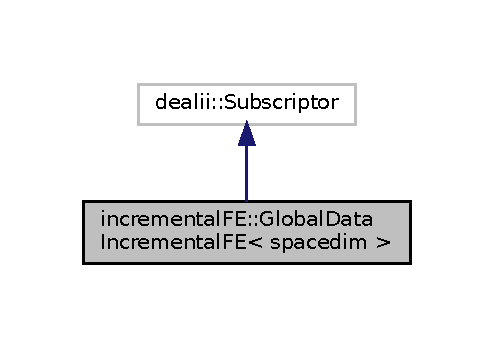
\includegraphics[width=220pt]{classincremental_f_e_1_1_global_data_incremental_f_e__inherit__graph}
\end{center}
\end{figure}


Collaboration diagram for incremental\+FE\+:\+:Global\+Data\+Incremental\+FE$<$ spacedim $>$\+:\nopagebreak
\begin{figure}[H]
\begin{center}
\leavevmode
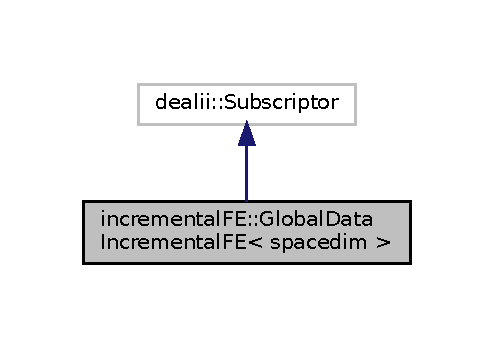
\includegraphics[width=220pt]{classincremental_f_e_1_1_global_data_incremental_f_e__coll__graph}
\end{center}
\end{figure}
\subsection*{Public Member Functions}
\begin{DoxyCompactItemize}
\item 
\hyperlink{classincremental_f_e_1_1_global_data_incremental_f_e_ac31163d303902de96e162419a1547495}{Global\+Data\+Incremental\+FE} (const double t\+\_\+init=0.\+0)
\item 
\hyperlink{classincremental_f_e_1_1_global_data_incremental_f_e_a718858c371f43d03f5d1c05560d62a9b}{$\sim$\+Global\+Data\+Incremental\+FE} ()
\item 
double \hyperlink{classincremental_f_e_1_1_global_data_incremental_f_e_af0064c4092b0dbb24817822c3104042f}{get\+\_\+t} () const 
\item 
double \hyperlink{classincremental_f_e_1_1_global_data_incremental_f_e_a81e09842fdcbc393a8bc9ccf3c0cdced}{get\+\_\+t\+\_\+ref} () const 
\item 
unsigned int \hyperlink{classincremental_f_e_1_1_global_data_incremental_f_e_a1d4f31e2249902397992cff85683c3b4}{get\+\_\+time\+\_\+step} () const 
\item 
void \hyperlink{classincremental_f_e_1_1_global_data_incremental_f_e_a9845e6a20c93b8aec769238ac23106da}{write\+\_\+error\+\_\+message} (const std\+::string error\+\_\+message)
\item 
void \hyperlink{classincremental_f_e_1_1_global_data_incremental_f_e_abf2246df069e3f8be4cd74467803159a}{write\+\_\+error\+\_\+message} (const std\+::string error\+\_\+message, const dealii\+::\+Point$<$ spacedim $>$ \&location)
\item 
void \hyperlink{classincremental_f_e_1_1_global_data_incremental_f_e_a3aaaf483ad4e6dbfc189e7ab2b44d21b}{print\+\_\+error\+\_\+messages} () const 
\item 
void \hyperlink{classincremental_f_e_1_1_global_data_incremental_f_e_a49d0b9cfe7b58e4f5e15e77733983d78}{print\+\_\+last\+\_\+error\+\_\+message} () const 
\item 
void \hyperlink{classincremental_f_e_1_1_global_data_incremental_f_e_a8378d6a77b65364d8036f8a111e86de0}{set\+\_\+sym\+\_\+mode} (const bool \hyperlink{classincremental_f_e_1_1_global_data_incremental_f_e_a9986ee5bfccc1b5936c585cf0c5a4474}{sym\+\_\+mode})
\item 
void \hyperlink{classincremental_f_e_1_1_global_data_incremental_f_e_a5b5ebd81c1da8af2321f79e44a89c9cf}{set\+\_\+max\+\_\+iter} (const unsigned int \hyperlink{classincremental_f_e_1_1_global_data_incremental_f_e_ad15c334652b6a9d6843c360c6e2005ec}{max\+\_\+iter})
\item 
void \hyperlink{classincremental_f_e_1_1_global_data_incremental_f_e_a892280978280b21be48bafed07d7c60a}{set\+\_\+max\+\_\+cutbacks} (const unsigned int \hyperlink{classincremental_f_e_1_1_global_data_incremental_f_e_a7ae58573e9cc241a14976bf19351ba63}{max\+\_\+cutbacks})
\item 
void \hyperlink{classincremental_f_e_1_1_global_data_incremental_f_e_a09f0851c50886a9f57996558c08fc108}{set\+\_\+threshold\+\_\+potential\+\_\+increment} (const double \hyperlink{classincremental_f_e_1_1_global_data_incremental_f_e_a2f7adb8b4f7f8875715e1dbd0edd9ac8}{threshold\+\_\+potential\+\_\+increment})
\item 
void \hyperlink{classincremental_f_e_1_1_global_data_incremental_f_e_aba65d5da0031c2f1bc1ceb87dc524b8d}{set\+\_\+force\+\_\+linear} (const bool \hyperlink{classincremental_f_e_1_1_global_data_incremental_f_e_a37c1d42902e74f13f3c4ba82d2dabd67}{force\+\_\+linear}=true)
\item 
void \hyperlink{classincremental_f_e_1_1_global_data_incremental_f_e_a82d4ae6026b8c8a4a4da1c54e81fd64a}{set\+\_\+predictor\+\_\+corrector} (const bool \hyperlink{classincremental_f_e_1_1_global_data_incremental_f_e_a5cc0d20e5e389c149bbd288f57dee953}{predictor\+\_\+corrector}=true)
\item 
bool \hyperlink{classincremental_f_e_1_1_global_data_incremental_f_e_a6814f2a2bf9f3369b9d1ea7ee8cab33a}{get\+\_\+predictor\+\_\+step} () const 
\item 
unsigned int \hyperlink{classincremental_f_e_1_1_global_data_incremental_f_e_a5d95155e9cc3cae28a5fbe7866f603d7}{get\+\_\+output\+\_\+level} () const 
\item 
void \hyperlink{classincremental_f_e_1_1_global_data_incremental_f_e_a44ec19d072819c3531be56ada4b7d077}{set\+\_\+output\+\_\+level} (const unsigned int \hyperlink{classincremental_f_e_1_1_global_data_incremental_f_e_a0d5cf3ecf70ec61771bbcfe45d0e6b5d}{output\+\_\+level})
\item 
void \hyperlink{classincremental_f_e_1_1_global_data_incremental_f_e_a916e33b7d8d6dcc1a113c130c995f8b3}{set\+\_\+safety\+\_\+distance} (const double \hyperlink{classincremental_f_e_1_1_global_data_incremental_f_e_a6db92e8e97c6875df1ecf5aa2a3a0345}{safety\+\_\+distance})
\item 
void \hyperlink{classincremental_f_e_1_1_global_data_incremental_f_e_a27354ebc5bf9ec655f5c7cc16ac9876d}{set\+\_\+t} (const double \hyperlink{classincremental_f_e_1_1_global_data_incremental_f_e_abb14e15389af3772905a3c75e12ed2c0}{t})
\item 
void \hyperlink{classincremental_f_e_1_1_global_data_incremental_f_e_ab86938372e460e4253c5cc22edffbf94}{reset\+\_\+t} ()
\item 
void \hyperlink{classincremental_f_e_1_1_global_data_incremental_f_e_ae8037538c6a7fc8b05168fe006ed2083}{set\+\_\+predictor\+\_\+step} (const bool \hyperlink{classincremental_f_e_1_1_global_data_incremental_f_e_afe172fdb882f9dd0cd5f963386dd2ffb}{predictor\+\_\+step}=true)
\item 
void \hyperlink{classincremental_f_e_1_1_global_data_incremental_f_e_ad3cd830a41c4b92c69d2083864ac7478}{set\+\_\+perform\+\_\+line\+\_\+search} (const bool \hyperlink{classincremental_f_e_1_1_global_data_incremental_f_e_a2253a9b142315cbccac38c8b8dc83824}{perform\+\_\+line\+\_\+search}=true)
\item 
void \hyperlink{classincremental_f_e_1_1_global_data_incremental_f_e_a74424d0040a6f5c2aa545288b42483f4}{reinit} (const double t\+\_\+init=0.\+0)
\end{DoxyCompactItemize}
\subsection*{Private Attributes}
\begin{DoxyCompactItemize}
\item 
double \hyperlink{classincremental_f_e_1_1_global_data_incremental_f_e_abb14e15389af3772905a3c75e12ed2c0}{t}
\item 
double \hyperlink{classincremental_f_e_1_1_global_data_incremental_f_e_a6ddf751a2f8abff9353d12e469e38f96}{t\+\_\+ref}
\item 
double \hyperlink{classincremental_f_e_1_1_global_data_incremental_f_e_ad808aad6cdbfa6eddad05fb85c056d11}{t\+\_\+ref\+\_\+old}
\item 
unsigned int \hyperlink{classincremental_f_e_1_1_global_data_incremental_f_e_a2aa7544464ad55c39f44c9e7e04b4bf6}{time\+\_\+step} = 0
\item 
bool \hyperlink{classincremental_f_e_1_1_global_data_incremental_f_e_a9986ee5bfccc1b5936c585cf0c5a4474}{sym\+\_\+mode} = false
\item 
unsigned int \hyperlink{classincremental_f_e_1_1_global_data_incremental_f_e_ad15c334652b6a9d6843c360c6e2005ec}{max\+\_\+iter} = 20
\item 
unsigned int \hyperlink{classincremental_f_e_1_1_global_data_incremental_f_e_a7ae58573e9cc241a14976bf19351ba63}{max\+\_\+cutbacks} = 10
\item 
double \hyperlink{classincremental_f_e_1_1_global_data_incremental_f_e_a2f7adb8b4f7f8875715e1dbd0edd9ac8}{threshold\+\_\+potential\+\_\+increment} = 1e-\/14
\item 
bool \hyperlink{classincremental_f_e_1_1_global_data_incremental_f_e_a37c1d42902e74f13f3c4ba82d2dabd67}{force\+\_\+linear} = false
\item 
std\+::vector$<$ std\+::string $>$ \hyperlink{classincremental_f_e_1_1_global_data_incremental_f_e_a47301f72bcb3852b2519b23de833f3eb}{error\+\_\+messages}
\item 
bool \hyperlink{classincremental_f_e_1_1_global_data_incremental_f_e_a23a3040aa83a8867ccb0a8e88bb8cb9e}{reset\+\_\+t\+\_\+possible} = false
\item 
bool \hyperlink{classincremental_f_e_1_1_global_data_incremental_f_e_a5cc0d20e5e389c149bbd288f57dee953}{predictor\+\_\+corrector} = false
\item 
bool \hyperlink{classincremental_f_e_1_1_global_data_incremental_f_e_afe172fdb882f9dd0cd5f963386dd2ffb}{predictor\+\_\+step} = false
\item 
double \hyperlink{classincremental_f_e_1_1_global_data_incremental_f_e_a6db92e8e97c6875df1ecf5aa2a3a0345}{safety\+\_\+distance} = 0.\+9
\item 
unsigned int \hyperlink{classincremental_f_e_1_1_global_data_incremental_f_e_a0d5cf3ecf70ec61771bbcfe45d0e6b5d}{output\+\_\+level} = 1
\item 
bool \hyperlink{classincremental_f_e_1_1_global_data_incremental_f_e_a2253a9b142315cbccac38c8b8dc83824}{perform\+\_\+line\+\_\+search} = true
\end{DoxyCompactItemize}
\subsection*{Friends}
\begin{DoxyCompactItemize}
\item 
{\footnotesize template$<$unsigned int, class Solution\+Vector\+Type , class R\+H\+S\+Vector\+Type , class Matrix\+Type $>$ }\\class \hyperlink{classincremental_f_e_1_1_global_data_incremental_f_e_a19042fe49657aad3a64c2a04565a12d8}{F\+E\+Model}
\end{DoxyCompactItemize}


\subsection{Detailed Description}
\subsubsection*{template$<$unsigned int spacedim$>$\\*
class incremental\+F\+E\+::\+Global\+Data\+Incremental\+F\+E$<$ spacedim $>$}

This class is used to store global data like time, reference time, time step number, iteration number, error messages, termination criteria, etc. for the solution of time dependent, non-\/linear problems.

In particular if objects of classes derived from {\bf Scalar\+Functional} or {\bf Scalar\+Functional$<$spacedim, spacedim$>$} know of the \hyperlink{classincremental_f_e_1_1_global_data_incremental_f_e}{Global\+Data\+Incremental\+FE} object in use, global information (e.\+g. the current time and the reference time) is available at the material point level. The latter is important for the implementation of time discrete schemes.

The \hyperlink{classincremental_f_e_1_1_global_data_incremental_f_e}{Global\+Data\+Incremental\+FE} class inherits from {\bf Subscriptor} in order to be able to check that \hyperlink{classincremental_f_e_1_1_global_data_incremental_f_e}{Global\+Data\+Incremental\+FE} objects are only destroyed when they are not needed anymore by other objects.


\begin{DoxyTemplParams}{Template Parameters}
{\em spacedim} & spatial dimension of the problem \\
\hline
\end{DoxyTemplParams}


\subsection{Constructor \& Destructor Documentation}
\index{incremental\+F\+E\+::\+Global\+Data\+Incremental\+FE@{incremental\+F\+E\+::\+Global\+Data\+Incremental\+FE}!Global\+Data\+Incremental\+FE@{Global\+Data\+Incremental\+FE}}
\index{Global\+Data\+Incremental\+FE@{Global\+Data\+Incremental\+FE}!incremental\+F\+E\+::\+Global\+Data\+Incremental\+FE@{incremental\+F\+E\+::\+Global\+Data\+Incremental\+FE}}
\subsubsection[{\texorpdfstring{Global\+Data\+Incremental\+F\+E(const double t\+\_\+init=0.\+0)}{GlobalDataIncrementalFE(const double t_init=0.0)}}]{\setlength{\rightskip}{0pt plus 5cm}template$<$unsigned int spacedim$>$ {\bf incremental\+F\+E\+::\+Global\+Data\+Incremental\+FE}$<$ spacedim $>$\+::{\bf Global\+Data\+Incremental\+FE} (
\begin{DoxyParamCaption}
\item[{const double}]{t\+\_\+init = {\ttfamily 0.0}}
\end{DoxyParamCaption}
)}\hypertarget{classincremental_f_e_1_1_global_data_incremental_f_e_ac31163d303902de96e162419a1547495}{}\label{classincremental_f_e_1_1_global_data_incremental_f_e_ac31163d303902de96e162419a1547495}
Constructor allowing to construct object with non-\/default initial time


\begin{DoxyParams}[1]{Parameters}
\mbox{\tt in}  & {\em t\+\_\+init} & initial time \\
\hline
\end{DoxyParams}
\index{incremental\+F\+E\+::\+Global\+Data\+Incremental\+FE@{incremental\+F\+E\+::\+Global\+Data\+Incremental\+FE}!````~Global\+Data\+Incremental\+FE@{$\sim$\+Global\+Data\+Incremental\+FE}}
\index{````~Global\+Data\+Incremental\+FE@{$\sim$\+Global\+Data\+Incremental\+FE}!incremental\+F\+E\+::\+Global\+Data\+Incremental\+FE@{incremental\+F\+E\+::\+Global\+Data\+Incremental\+FE}}
\subsubsection[{\texorpdfstring{$\sim$\+Global\+Data\+Incremental\+F\+E()}{~GlobalDataIncrementalFE()}}]{\setlength{\rightskip}{0pt plus 5cm}template$<$unsigned int spacedim$>$ {\bf incremental\+F\+E\+::\+Global\+Data\+Incremental\+FE}$<$ spacedim $>$\+::$\sim${\bf Global\+Data\+Incremental\+FE} (
\begin{DoxyParamCaption}
{}
\end{DoxyParamCaption}
)}\hypertarget{classincremental_f_e_1_1_global_data_incremental_f_e_a718858c371f43d03f5d1c05560d62a9b}{}\label{classincremental_f_e_1_1_global_data_incremental_f_e_a718858c371f43d03f5d1c05560d62a9b}
The destructor of \hyperlink{classincremental_f_e_1_1_global_data_incremental_f_e}{Global\+Data\+Incremental\+FE} essentially checks before destruction that the \hyperlink{classincremental_f_e_1_1_global_data_incremental_f_e}{Global\+Data\+Incremental\+FE} object is not used by other objects. If this is the case, the program will be aborted. 

\subsection{Member Function Documentation}
\index{incremental\+F\+E\+::\+Global\+Data\+Incremental\+FE@{incremental\+F\+E\+::\+Global\+Data\+Incremental\+FE}!get\+\_\+output\+\_\+level@{get\+\_\+output\+\_\+level}}
\index{get\+\_\+output\+\_\+level@{get\+\_\+output\+\_\+level}!incremental\+F\+E\+::\+Global\+Data\+Incremental\+FE@{incremental\+F\+E\+::\+Global\+Data\+Incremental\+FE}}
\subsubsection[{\texorpdfstring{get\+\_\+output\+\_\+level() const }{get_output_level() const }}]{\setlength{\rightskip}{0pt plus 5cm}template$<$unsigned int spacedim$>$ unsigned int {\bf incremental\+F\+E\+::\+Global\+Data\+Incremental\+FE}$<$ spacedim $>$\+::get\+\_\+output\+\_\+level (
\begin{DoxyParamCaption}
{}
\end{DoxyParamCaption}
) const}\hypertarget{classincremental_f_e_1_1_global_data_incremental_f_e_a5d95155e9cc3cae28a5fbe7866f603d7}{}\label{classincremental_f_e_1_1_global_data_incremental_f_e_a5d95155e9cc3cae28a5fbe7866f603d7}
\begin{DoxyReturn}{Returns}
\hyperlink{classincremental_f_e_1_1_global_data_incremental_f_e_a0d5cf3ecf70ec61771bbcfe45d0e6b5d}{Global\+Data\+Incremental\+F\+E\+::output\+\_\+level} 
\end{DoxyReturn}
\index{incremental\+F\+E\+::\+Global\+Data\+Incremental\+FE@{incremental\+F\+E\+::\+Global\+Data\+Incremental\+FE}!get\+\_\+predictor\+\_\+step@{get\+\_\+predictor\+\_\+step}}
\index{get\+\_\+predictor\+\_\+step@{get\+\_\+predictor\+\_\+step}!incremental\+F\+E\+::\+Global\+Data\+Incremental\+FE@{incremental\+F\+E\+::\+Global\+Data\+Incremental\+FE}}
\subsubsection[{\texorpdfstring{get\+\_\+predictor\+\_\+step() const }{get_predictor_step() const }}]{\setlength{\rightskip}{0pt plus 5cm}template$<$unsigned int spacedim$>$ bool {\bf incremental\+F\+E\+::\+Global\+Data\+Incremental\+FE}$<$ spacedim $>$\+::get\+\_\+predictor\+\_\+step (
\begin{DoxyParamCaption}
{}
\end{DoxyParamCaption}
) const}\hypertarget{classincremental_f_e_1_1_global_data_incremental_f_e_a6814f2a2bf9f3369b9d1ea7ee8cab33a}{}\label{classincremental_f_e_1_1_global_data_incremental_f_e_a6814f2a2bf9f3369b9d1ea7ee8cab33a}
\begin{DoxyReturn}{Returns}
\hyperlink{classincremental_f_e_1_1_global_data_incremental_f_e_afe172fdb882f9dd0cd5f963386dd2ffb}{Global\+Data\+Incremental\+F\+E\+::predictor\+\_\+step} 
\end{DoxyReturn}
\index{incremental\+F\+E\+::\+Global\+Data\+Incremental\+FE@{incremental\+F\+E\+::\+Global\+Data\+Incremental\+FE}!get\+\_\+t@{get\+\_\+t}}
\index{get\+\_\+t@{get\+\_\+t}!incremental\+F\+E\+::\+Global\+Data\+Incremental\+FE@{incremental\+F\+E\+::\+Global\+Data\+Incremental\+FE}}
\subsubsection[{\texorpdfstring{get\+\_\+t() const }{get_t() const }}]{\setlength{\rightskip}{0pt plus 5cm}template$<$unsigned int spacedim$>$ double {\bf incremental\+F\+E\+::\+Global\+Data\+Incremental\+FE}$<$ spacedim $>$\+::get\+\_\+t (
\begin{DoxyParamCaption}
{}
\end{DoxyParamCaption}
) const}\hypertarget{classincremental_f_e_1_1_global_data_incremental_f_e_af0064c4092b0dbb24817822c3104042f}{}\label{classincremental_f_e_1_1_global_data_incremental_f_e_af0064c4092b0dbb24817822c3104042f}
\begin{DoxyReturn}{Returns}
The current time \hyperlink{classincremental_f_e_1_1_global_data_incremental_f_e_abb14e15389af3772905a3c75e12ed2c0}{Global\+Data\+Incremental\+F\+E\+::t} 
\end{DoxyReturn}
\index{incremental\+F\+E\+::\+Global\+Data\+Incremental\+FE@{incremental\+F\+E\+::\+Global\+Data\+Incremental\+FE}!get\+\_\+t\+\_\+ref@{get\+\_\+t\+\_\+ref}}
\index{get\+\_\+t\+\_\+ref@{get\+\_\+t\+\_\+ref}!incremental\+F\+E\+::\+Global\+Data\+Incremental\+FE@{incremental\+F\+E\+::\+Global\+Data\+Incremental\+FE}}
\subsubsection[{\texorpdfstring{get\+\_\+t\+\_\+ref() const }{get_t_ref() const }}]{\setlength{\rightskip}{0pt plus 5cm}template$<$unsigned int spacedim$>$ double {\bf incremental\+F\+E\+::\+Global\+Data\+Incremental\+FE}$<$ spacedim $>$\+::get\+\_\+t\+\_\+ref (
\begin{DoxyParamCaption}
{}
\end{DoxyParamCaption}
) const}\hypertarget{classincremental_f_e_1_1_global_data_incremental_f_e_a81e09842fdcbc393a8bc9ccf3c0cdced}{}\label{classincremental_f_e_1_1_global_data_incremental_f_e_a81e09842fdcbc393a8bc9ccf3c0cdced}
\begin{DoxyReturn}{Returns}
The reference time \hyperlink{classincremental_f_e_1_1_global_data_incremental_f_e_a6ddf751a2f8abff9353d12e469e38f96}{Global\+Data\+Incremental\+F\+E\+::t\+\_\+ref} 
\end{DoxyReturn}
\index{incremental\+F\+E\+::\+Global\+Data\+Incremental\+FE@{incremental\+F\+E\+::\+Global\+Data\+Incremental\+FE}!get\+\_\+time\+\_\+step@{get\+\_\+time\+\_\+step}}
\index{get\+\_\+time\+\_\+step@{get\+\_\+time\+\_\+step}!incremental\+F\+E\+::\+Global\+Data\+Incremental\+FE@{incremental\+F\+E\+::\+Global\+Data\+Incremental\+FE}}
\subsubsection[{\texorpdfstring{get\+\_\+time\+\_\+step() const }{get_time_step() const }}]{\setlength{\rightskip}{0pt plus 5cm}template$<$unsigned int spacedim$>$ unsigned int {\bf incremental\+F\+E\+::\+Global\+Data\+Incremental\+FE}$<$ spacedim $>$\+::get\+\_\+time\+\_\+step (
\begin{DoxyParamCaption}
{}
\end{DoxyParamCaption}
) const}\hypertarget{classincremental_f_e_1_1_global_data_incremental_f_e_a1d4f31e2249902397992cff85683c3b4}{}\label{classincremental_f_e_1_1_global_data_incremental_f_e_a1d4f31e2249902397992cff85683c3b4}
\begin{DoxyReturn}{Returns}
current time step number \hyperlink{classincremental_f_e_1_1_global_data_incremental_f_e_a2aa7544464ad55c39f44c9e7e04b4bf6}{Global\+Data\+Incremental\+F\+E\+::time\+\_\+step} 
\end{DoxyReturn}
\index{incremental\+F\+E\+::\+Global\+Data\+Incremental\+FE@{incremental\+F\+E\+::\+Global\+Data\+Incremental\+FE}!print\+\_\+error\+\_\+messages@{print\+\_\+error\+\_\+messages}}
\index{print\+\_\+error\+\_\+messages@{print\+\_\+error\+\_\+messages}!incremental\+F\+E\+::\+Global\+Data\+Incremental\+FE@{incremental\+F\+E\+::\+Global\+Data\+Incremental\+FE}}
\subsubsection[{\texorpdfstring{print\+\_\+error\+\_\+messages() const }{print_error_messages() const }}]{\setlength{\rightskip}{0pt plus 5cm}template$<$unsigned int spacedim$>$ void {\bf incremental\+F\+E\+::\+Global\+Data\+Incremental\+FE}$<$ spacedim $>$\+::print\+\_\+error\+\_\+messages (
\begin{DoxyParamCaption}
{}
\end{DoxyParamCaption}
) const}\hypertarget{classincremental_f_e_1_1_global_data_incremental_f_e_a3aaaf483ad4e6dbfc189e7ab2b44d21b}{}\label{classincremental_f_e_1_1_global_data_incremental_f_e_a3aaaf483ad4e6dbfc189e7ab2b44d21b}
Function to print error messages to screen \index{incremental\+F\+E\+::\+Global\+Data\+Incremental\+FE@{incremental\+F\+E\+::\+Global\+Data\+Incremental\+FE}!print\+\_\+last\+\_\+error\+\_\+message@{print\+\_\+last\+\_\+error\+\_\+message}}
\index{print\+\_\+last\+\_\+error\+\_\+message@{print\+\_\+last\+\_\+error\+\_\+message}!incremental\+F\+E\+::\+Global\+Data\+Incremental\+FE@{incremental\+F\+E\+::\+Global\+Data\+Incremental\+FE}}
\subsubsection[{\texorpdfstring{print\+\_\+last\+\_\+error\+\_\+message() const }{print_last_error_message() const }}]{\setlength{\rightskip}{0pt plus 5cm}template$<$unsigned int spacedim$>$ void {\bf incremental\+F\+E\+::\+Global\+Data\+Incremental\+FE}$<$ spacedim $>$\+::print\+\_\+last\+\_\+error\+\_\+message (
\begin{DoxyParamCaption}
{}
\end{DoxyParamCaption}
) const}\hypertarget{classincremental_f_e_1_1_global_data_incremental_f_e_a49d0b9cfe7b58e4f5e15e77733983d78}{}\label{classincremental_f_e_1_1_global_data_incremental_f_e_a49d0b9cfe7b58e4f5e15e77733983d78}
Function to print last error message to screen \index{incremental\+F\+E\+::\+Global\+Data\+Incremental\+FE@{incremental\+F\+E\+::\+Global\+Data\+Incremental\+FE}!reinit@{reinit}}
\index{reinit@{reinit}!incremental\+F\+E\+::\+Global\+Data\+Incremental\+FE@{incremental\+F\+E\+::\+Global\+Data\+Incremental\+FE}}
\subsubsection[{\texorpdfstring{reinit(const double t\+\_\+init=0.\+0)}{reinit(const double t_init=0.0)}}]{\setlength{\rightskip}{0pt plus 5cm}template$<$unsigned int spacedim$>$ void {\bf incremental\+F\+E\+::\+Global\+Data\+Incremental\+FE}$<$ spacedim $>$\+::reinit (
\begin{DoxyParamCaption}
\item[{const double}]{t\+\_\+init = {\ttfamily 0.0}}
\end{DoxyParamCaption}
)}\hypertarget{classincremental_f_e_1_1_global_data_incremental_f_e_a74424d0040a6f5c2aa545288b42483f4}{}\label{classincremental_f_e_1_1_global_data_incremental_f_e_a74424d0040a6f5c2aa545288b42483f4}
reset \hyperlink{classincremental_f_e_1_1_global_data_incremental_f_e_abb14e15389af3772905a3c75e12ed2c0}{Global\+Data\+Incremental\+F\+E\+::t}, \hyperlink{classincremental_f_e_1_1_global_data_incremental_f_e_a6ddf751a2f8abff9353d12e469e38f96}{Global\+Data\+Incremental\+F\+E\+::t\+\_\+ref}, \hyperlink{classincremental_f_e_1_1_global_data_incremental_f_e_ad808aad6cdbfa6eddad05fb85c056d11}{Global\+Data\+Incremental\+F\+E\+::t\+\_\+ref\+\_\+old}, \hyperlink{classincremental_f_e_1_1_global_data_incremental_f_e_a2aa7544464ad55c39f44c9e7e04b4bf6}{Global\+Data\+Incremental\+F\+E\+::time\+\_\+step}, \hyperlink{classincremental_f_e_1_1_global_data_incremental_f_e_a47301f72bcb3852b2519b23de833f3eb}{Global\+Data\+Incremental\+F\+E\+::error\+\_\+messages}


\begin{DoxyParams}[1]{Parameters}
\mbox{\tt in}  & {\em t\+\_\+init} & time to be used for resetting \hyperlink{classincremental_f_e_1_1_global_data_incremental_f_e_abb14e15389af3772905a3c75e12ed2c0}{Global\+Data\+Incremental\+F\+E\+::t}, \hyperlink{classincremental_f_e_1_1_global_data_incremental_f_e_a6ddf751a2f8abff9353d12e469e38f96}{Global\+Data\+Incremental\+F\+E\+::t\+\_\+ref}, \hyperlink{classincremental_f_e_1_1_global_data_incremental_f_e_ad808aad6cdbfa6eddad05fb85c056d11}{Global\+Data\+Incremental\+F\+E\+::t\+\_\+ref\+\_\+old} \\
\hline
\end{DoxyParams}
\index{incremental\+F\+E\+::\+Global\+Data\+Incremental\+FE@{incremental\+F\+E\+::\+Global\+Data\+Incremental\+FE}!reset\+\_\+t@{reset\+\_\+t}}
\index{reset\+\_\+t@{reset\+\_\+t}!incremental\+F\+E\+::\+Global\+Data\+Incremental\+FE@{incremental\+F\+E\+::\+Global\+Data\+Incremental\+FE}}
\subsubsection[{\texorpdfstring{reset\+\_\+t()}{reset_t()}}]{\setlength{\rightskip}{0pt plus 5cm}template$<$unsigned int spacedim$>$ void {\bf incremental\+F\+E\+::\+Global\+Data\+Incremental\+FE}$<$ spacedim $>$\+::reset\+\_\+t (
\begin{DoxyParamCaption}
{}
\end{DoxyParamCaption}
)}\hypertarget{classincremental_f_e_1_1_global_data_incremental_f_e_ab86938372e460e4253c5cc22edffbf94}{}\label{classincremental_f_e_1_1_global_data_incremental_f_e_ab86938372e460e4253c5cc22edffbf94}
Function resetting time to previous step. This undoes the last call to \hyperlink{classincremental_f_e_1_1_global_data_incremental_f_e_a27354ebc5bf9ec655f5c7cc16ac9876d}{Global\+Data\+Incremental\+F\+E\+::set\+\_\+t()}. The function can only be called once after a call of \hyperlink{classincremental_f_e_1_1_global_data_incremental_f_e_a27354ebc5bf9ec655f5c7cc16ac9876d}{Global\+Data\+Incremental\+F\+E\+::set\+\_\+t()}. \index{incremental\+F\+E\+::\+Global\+Data\+Incremental\+FE@{incremental\+F\+E\+::\+Global\+Data\+Incremental\+FE}!set\+\_\+force\+\_\+linear@{set\+\_\+force\+\_\+linear}}
\index{set\+\_\+force\+\_\+linear@{set\+\_\+force\+\_\+linear}!incremental\+F\+E\+::\+Global\+Data\+Incremental\+FE@{incremental\+F\+E\+::\+Global\+Data\+Incremental\+FE}}
\subsubsection[{\texorpdfstring{set\+\_\+force\+\_\+linear(const bool force\+\_\+linear=true)}{set_force_linear(const bool force_linear=true)}}]{\setlength{\rightskip}{0pt plus 5cm}template$<$unsigned int spacedim$>$ void {\bf incremental\+F\+E\+::\+Global\+Data\+Incremental\+FE}$<$ spacedim $>$\+::set\+\_\+force\+\_\+linear (
\begin{DoxyParamCaption}
\item[{const bool}]{force\+\_\+linear = {\ttfamily true}}
\end{DoxyParamCaption}
)}\hypertarget{classincremental_f_e_1_1_global_data_incremental_f_e_aba65d5da0031c2f1bc1ceb87dc524b8d}{}\label{classincremental_f_e_1_1_global_data_incremental_f_e_aba65d5da0031c2f1bc1ceb87dc524b8d}
Sets \hyperlink{classincremental_f_e_1_1_global_data_incremental_f_e_a37c1d42902e74f13f3c4ba82d2dabd67}{Global\+Data\+Incremental\+F\+E\+::force\+\_\+linear}


\begin{DoxyParams}[1]{Parameters}
\mbox{\tt in}  & {\em force\+\_\+linear} & \hyperlink{classincremental_f_e_1_1_global_data_incremental_f_e_a37c1d42902e74f13f3c4ba82d2dabd67}{Global\+Data\+Incremental\+F\+E\+::force\+\_\+linear} \\
\hline
\end{DoxyParams}
\index{incremental\+F\+E\+::\+Global\+Data\+Incremental\+FE@{incremental\+F\+E\+::\+Global\+Data\+Incremental\+FE}!set\+\_\+max\+\_\+cutbacks@{set\+\_\+max\+\_\+cutbacks}}
\index{set\+\_\+max\+\_\+cutbacks@{set\+\_\+max\+\_\+cutbacks}!incremental\+F\+E\+::\+Global\+Data\+Incremental\+FE@{incremental\+F\+E\+::\+Global\+Data\+Incremental\+FE}}
\subsubsection[{\texorpdfstring{set\+\_\+max\+\_\+cutbacks(const unsigned int max\+\_\+cutbacks)}{set_max_cutbacks(const unsigned int max_cutbacks)}}]{\setlength{\rightskip}{0pt plus 5cm}template$<$unsigned int spacedim$>$ void {\bf incremental\+F\+E\+::\+Global\+Data\+Incremental\+FE}$<$ spacedim $>$\+::set\+\_\+max\+\_\+cutbacks (
\begin{DoxyParamCaption}
\item[{const unsigned int}]{max\+\_\+cutbacks}
\end{DoxyParamCaption}
)}\hypertarget{classincremental_f_e_1_1_global_data_incremental_f_e_a892280978280b21be48bafed07d7c60a}{}\label{classincremental_f_e_1_1_global_data_incremental_f_e_a892280978280b21be48bafed07d7c60a}
Sets \hyperlink{classincremental_f_e_1_1_global_data_incremental_f_e_a7ae58573e9cc241a14976bf19351ba63}{Global\+Data\+Incremental\+F\+E\+::max\+\_\+cutbacks}


\begin{DoxyParams}[1]{Parameters}
\mbox{\tt in}  & {\em max\+\_\+cutbacks} & \hyperlink{classincremental_f_e_1_1_global_data_incremental_f_e_a7ae58573e9cc241a14976bf19351ba63}{Global\+Data\+Incremental\+F\+E\+::max\+\_\+cutbacks} \\
\hline
\end{DoxyParams}
\index{incremental\+F\+E\+::\+Global\+Data\+Incremental\+FE@{incremental\+F\+E\+::\+Global\+Data\+Incremental\+FE}!set\+\_\+max\+\_\+iter@{set\+\_\+max\+\_\+iter}}
\index{set\+\_\+max\+\_\+iter@{set\+\_\+max\+\_\+iter}!incremental\+F\+E\+::\+Global\+Data\+Incremental\+FE@{incremental\+F\+E\+::\+Global\+Data\+Incremental\+FE}}
\subsubsection[{\texorpdfstring{set\+\_\+max\+\_\+iter(const unsigned int max\+\_\+iter)}{set_max_iter(const unsigned int max_iter)}}]{\setlength{\rightskip}{0pt plus 5cm}template$<$unsigned int spacedim$>$ void {\bf incremental\+F\+E\+::\+Global\+Data\+Incremental\+FE}$<$ spacedim $>$\+::set\+\_\+max\+\_\+iter (
\begin{DoxyParamCaption}
\item[{const unsigned int}]{max\+\_\+iter}
\end{DoxyParamCaption}
)}\hypertarget{classincremental_f_e_1_1_global_data_incremental_f_e_a5b5ebd81c1da8af2321f79e44a89c9cf}{}\label{classincremental_f_e_1_1_global_data_incremental_f_e_a5b5ebd81c1da8af2321f79e44a89c9cf}
Sets \hyperlink{classincremental_f_e_1_1_global_data_incremental_f_e_ad15c334652b6a9d6843c360c6e2005ec}{Global\+Data\+Incremental\+F\+E\+::max\+\_\+iter}


\begin{DoxyParams}[1]{Parameters}
\mbox{\tt in}  & {\em max\+\_\+iter} & \hyperlink{classincremental_f_e_1_1_global_data_incremental_f_e_ad15c334652b6a9d6843c360c6e2005ec}{Global\+Data\+Incremental\+F\+E\+::max\+\_\+iter} \\
\hline
\end{DoxyParams}
\index{incremental\+F\+E\+::\+Global\+Data\+Incremental\+FE@{incremental\+F\+E\+::\+Global\+Data\+Incremental\+FE}!set\+\_\+output\+\_\+level@{set\+\_\+output\+\_\+level}}
\index{set\+\_\+output\+\_\+level@{set\+\_\+output\+\_\+level}!incremental\+F\+E\+::\+Global\+Data\+Incremental\+FE@{incremental\+F\+E\+::\+Global\+Data\+Incremental\+FE}}
\subsubsection[{\texorpdfstring{set\+\_\+output\+\_\+level(const unsigned int output\+\_\+level)}{set_output_level(const unsigned int output_level)}}]{\setlength{\rightskip}{0pt plus 5cm}template$<$unsigned int spacedim$>$ void {\bf incremental\+F\+E\+::\+Global\+Data\+Incremental\+FE}$<$ spacedim $>$\+::set\+\_\+output\+\_\+level (
\begin{DoxyParamCaption}
\item[{const unsigned int}]{output\+\_\+level}
\end{DoxyParamCaption}
)}\hypertarget{classincremental_f_e_1_1_global_data_incremental_f_e_a44ec19d072819c3531be56ada4b7d077}{}\label{classincremental_f_e_1_1_global_data_incremental_f_e_a44ec19d072819c3531be56ada4b7d077}
Sets \hyperlink{classincremental_f_e_1_1_global_data_incremental_f_e_a0d5cf3ecf70ec61771bbcfe45d0e6b5d}{Global\+Data\+Incremental\+F\+E\+::output\+\_\+level}


\begin{DoxyParams}[1]{Parameters}
\mbox{\tt in}  & {\em output\+\_\+level} & \hyperlink{classincremental_f_e_1_1_global_data_incremental_f_e_a0d5cf3ecf70ec61771bbcfe45d0e6b5d}{Global\+Data\+Incremental\+F\+E\+::output\+\_\+level} \\
\hline
\end{DoxyParams}
\index{incremental\+F\+E\+::\+Global\+Data\+Incremental\+FE@{incremental\+F\+E\+::\+Global\+Data\+Incremental\+FE}!set\+\_\+perform\+\_\+line\+\_\+search@{set\+\_\+perform\+\_\+line\+\_\+search}}
\index{set\+\_\+perform\+\_\+line\+\_\+search@{set\+\_\+perform\+\_\+line\+\_\+search}!incremental\+F\+E\+::\+Global\+Data\+Incremental\+FE@{incremental\+F\+E\+::\+Global\+Data\+Incremental\+FE}}
\subsubsection[{\texorpdfstring{set\+\_\+perform\+\_\+line\+\_\+search(const bool perform\+\_\+line\+\_\+search=true)}{set_perform_line_search(const bool perform_line_search=true)}}]{\setlength{\rightskip}{0pt plus 5cm}template$<$unsigned int spacedim$>$ void {\bf incremental\+F\+E\+::\+Global\+Data\+Incremental\+FE}$<$ spacedim $>$\+::set\+\_\+perform\+\_\+line\+\_\+search (
\begin{DoxyParamCaption}
\item[{const bool}]{perform\+\_\+line\+\_\+search = {\ttfamily true}}
\end{DoxyParamCaption}
)}\hypertarget{classincremental_f_e_1_1_global_data_incremental_f_e_ad3cd830a41c4b92c69d2083864ac7478}{}\label{classincremental_f_e_1_1_global_data_incremental_f_e_ad3cd830a41c4b92c69d2083864ac7478}
Sets \hyperlink{classincremental_f_e_1_1_global_data_incremental_f_e_a2253a9b142315cbccac38c8b8dc83824}{Global\+Data\+Incremental\+F\+E\+::perform\+\_\+line\+\_\+search}


\begin{DoxyParams}[1]{Parameters}
\mbox{\tt in}  & {\em perform\+\_\+line\+\_\+search} & \hyperlink{classincremental_f_e_1_1_global_data_incremental_f_e_a2253a9b142315cbccac38c8b8dc83824}{Global\+Data\+Incremental\+F\+E\+::perform\+\_\+line\+\_\+search} \\
\hline
\end{DoxyParams}
\index{incremental\+F\+E\+::\+Global\+Data\+Incremental\+FE@{incremental\+F\+E\+::\+Global\+Data\+Incremental\+FE}!set\+\_\+predictor\+\_\+corrector@{set\+\_\+predictor\+\_\+corrector}}
\index{set\+\_\+predictor\+\_\+corrector@{set\+\_\+predictor\+\_\+corrector}!incremental\+F\+E\+::\+Global\+Data\+Incremental\+FE@{incremental\+F\+E\+::\+Global\+Data\+Incremental\+FE}}
\subsubsection[{\texorpdfstring{set\+\_\+predictor\+\_\+corrector(const bool predictor\+\_\+corrector=true)}{set_predictor_corrector(const bool predictor_corrector=true)}}]{\setlength{\rightskip}{0pt plus 5cm}template$<$unsigned int spacedim$>$ void {\bf incremental\+F\+E\+::\+Global\+Data\+Incremental\+FE}$<$ spacedim $>$\+::set\+\_\+predictor\+\_\+corrector (
\begin{DoxyParamCaption}
\item[{const bool}]{predictor\+\_\+corrector = {\ttfamily true}}
\end{DoxyParamCaption}
)}\hypertarget{classincremental_f_e_1_1_global_data_incremental_f_e_a82d4ae6026b8c8a4a4da1c54e81fd64a}{}\label{classincremental_f_e_1_1_global_data_incremental_f_e_a82d4ae6026b8c8a4a4da1c54e81fd64a}
Sets \hyperlink{classincremental_f_e_1_1_global_data_incremental_f_e_a5cc0d20e5e389c149bbd288f57dee953}{Global\+Data\+Incremental\+F\+E\+::predictor\+\_\+corrector}


\begin{DoxyParams}[1]{Parameters}
\mbox{\tt in}  & {\em predictor\+\_\+corrector} & Indicate whether predictor-\/corrector algorithm is to be used \\
\hline
\end{DoxyParams}
\index{incremental\+F\+E\+::\+Global\+Data\+Incremental\+FE@{incremental\+F\+E\+::\+Global\+Data\+Incremental\+FE}!set\+\_\+predictor\+\_\+step@{set\+\_\+predictor\+\_\+step}}
\index{set\+\_\+predictor\+\_\+step@{set\+\_\+predictor\+\_\+step}!incremental\+F\+E\+::\+Global\+Data\+Incremental\+FE@{incremental\+F\+E\+::\+Global\+Data\+Incremental\+FE}}
\subsubsection[{\texorpdfstring{set\+\_\+predictor\+\_\+step(const bool predictor\+\_\+step=true)}{set_predictor_step(const bool predictor_step=true)}}]{\setlength{\rightskip}{0pt plus 5cm}template$<$unsigned int spacedim$>$ void {\bf incremental\+F\+E\+::\+Global\+Data\+Incremental\+FE}$<$ spacedim $>$\+::set\+\_\+predictor\+\_\+step (
\begin{DoxyParamCaption}
\item[{const bool}]{predictor\+\_\+step = {\ttfamily true}}
\end{DoxyParamCaption}
)}\hypertarget{classincremental_f_e_1_1_global_data_incremental_f_e_ae8037538c6a7fc8b05168fe006ed2083}{}\label{classincremental_f_e_1_1_global_data_incremental_f_e_ae8037538c6a7fc8b05168fe006ed2083}
Sets \hyperlink{classincremental_f_e_1_1_global_data_incremental_f_e_afe172fdb882f9dd0cd5f963386dd2ffb}{Global\+Data\+Incremental\+F\+E\+::predictor\+\_\+step}


\begin{DoxyParams}[1]{Parameters}
\mbox{\tt in}  & {\em predictor\+\_\+step} & \hyperlink{classincremental_f_e_1_1_global_data_incremental_f_e_afe172fdb882f9dd0cd5f963386dd2ffb}{Global\+Data\+Incremental\+F\+E\+::predictor\+\_\+step} \\
\hline
\end{DoxyParams}
\index{incremental\+F\+E\+::\+Global\+Data\+Incremental\+FE@{incremental\+F\+E\+::\+Global\+Data\+Incremental\+FE}!set\+\_\+safety\+\_\+distance@{set\+\_\+safety\+\_\+distance}}
\index{set\+\_\+safety\+\_\+distance@{set\+\_\+safety\+\_\+distance}!incremental\+F\+E\+::\+Global\+Data\+Incremental\+FE@{incremental\+F\+E\+::\+Global\+Data\+Incremental\+FE}}
\subsubsection[{\texorpdfstring{set\+\_\+safety\+\_\+distance(const double safety\+\_\+distance)}{set_safety_distance(const double safety_distance)}}]{\setlength{\rightskip}{0pt plus 5cm}template$<$unsigned int spacedim$>$ void {\bf incremental\+F\+E\+::\+Global\+Data\+Incremental\+FE}$<$ spacedim $>$\+::set\+\_\+safety\+\_\+distance (
\begin{DoxyParamCaption}
\item[{const double}]{safety\+\_\+distance}
\end{DoxyParamCaption}
)}\hypertarget{classincremental_f_e_1_1_global_data_incremental_f_e_a916e33b7d8d6dcc1a113c130c995f8b3}{}\label{classincremental_f_e_1_1_global_data_incremental_f_e_a916e33b7d8d6dcc1a113c130c995f8b3}
Sets \hyperlink{classincremental_f_e_1_1_global_data_incremental_f_e_a6db92e8e97c6875df1ecf5aa2a3a0345}{Global\+Data\+Incremental\+F\+E\+::safety\+\_\+distance}


\begin{DoxyParams}[1]{Parameters}
\mbox{\tt in}  & {\em safety\+\_\+distance} & \hyperlink{classincremental_f_e_1_1_global_data_incremental_f_e_a6db92e8e97c6875df1ecf5aa2a3a0345}{Global\+Data\+Incremental\+F\+E\+::safety\+\_\+distance} \\
\hline
\end{DoxyParams}
\index{incremental\+F\+E\+::\+Global\+Data\+Incremental\+FE@{incremental\+F\+E\+::\+Global\+Data\+Incremental\+FE}!set\+\_\+sym\+\_\+mode@{set\+\_\+sym\+\_\+mode}}
\index{set\+\_\+sym\+\_\+mode@{set\+\_\+sym\+\_\+mode}!incremental\+F\+E\+::\+Global\+Data\+Incremental\+FE@{incremental\+F\+E\+::\+Global\+Data\+Incremental\+FE}}
\subsubsection[{\texorpdfstring{set\+\_\+sym\+\_\+mode(const bool sym\+\_\+mode)}{set_sym_mode(const bool sym_mode)}}]{\setlength{\rightskip}{0pt plus 5cm}template$<$unsigned int spacedim$>$ void {\bf incremental\+F\+E\+::\+Global\+Data\+Incremental\+FE}$<$ spacedim $>$\+::set\+\_\+sym\+\_\+mode (
\begin{DoxyParamCaption}
\item[{const bool}]{sym\+\_\+mode}
\end{DoxyParamCaption}
)}\hypertarget{classincremental_f_e_1_1_global_data_incremental_f_e_a8378d6a77b65364d8036f8a111e86de0}{}\label{classincremental_f_e_1_1_global_data_incremental_f_e_a8378d6a77b65364d8036f8a111e86de0}
Sets \hyperlink{classincremental_f_e_1_1_global_data_incremental_f_e_a9986ee5bfccc1b5936c585cf0c5a4474}{Global\+Data\+Incremental\+F\+E\+::sym\+\_\+mode}


\begin{DoxyParams}[1]{Parameters}
\mbox{\tt in}  & {\em sym\+\_\+mode} & \hyperlink{classincremental_f_e_1_1_global_data_incremental_f_e_a9986ee5bfccc1b5936c585cf0c5a4474}{Global\+Data\+Incremental\+F\+E\+::sym\+\_\+mode} \\
\hline
\end{DoxyParams}
\index{incremental\+F\+E\+::\+Global\+Data\+Incremental\+FE@{incremental\+F\+E\+::\+Global\+Data\+Incremental\+FE}!set\+\_\+t@{set\+\_\+t}}
\index{set\+\_\+t@{set\+\_\+t}!incremental\+F\+E\+::\+Global\+Data\+Incremental\+FE@{incremental\+F\+E\+::\+Global\+Data\+Incremental\+FE}}
\subsubsection[{\texorpdfstring{set\+\_\+t(const double t)}{set_t(const double t)}}]{\setlength{\rightskip}{0pt plus 5cm}template$<$unsigned int spacedim$>$ void {\bf incremental\+F\+E\+::\+Global\+Data\+Incremental\+FE}$<$ spacedim $>$\+::set\+\_\+t (
\begin{DoxyParamCaption}
\item[{const double}]{t}
\end{DoxyParamCaption}
)}\hypertarget{classincremental_f_e_1_1_global_data_incremental_f_e_a27354ebc5bf9ec655f5c7cc16ac9876d}{}\label{classincremental_f_e_1_1_global_data_incremental_f_e_a27354ebc5bf9ec655f5c7cc16ac9876d}
Function setting current time (old time is then stored in \hyperlink{classincremental_f_e_1_1_global_data_incremental_f_e_a6ddf751a2f8abff9353d12e469e38f96}{Global\+Data\+Incremental\+F\+E\+::t\+\_\+ref}). This function also increments the time step number \hyperlink{classincremental_f_e_1_1_global_data_incremental_f_e_a2aa7544464ad55c39f44c9e7e04b4bf6}{Global\+Data\+Incremental\+F\+E\+::time\+\_\+step} and checks that the new time is larger than the old time.


\begin{DoxyParams}[1]{Parameters}
\mbox{\tt in}  & {\em t} & current time \\
\hline
\end{DoxyParams}
\index{incremental\+F\+E\+::\+Global\+Data\+Incremental\+FE@{incremental\+F\+E\+::\+Global\+Data\+Incremental\+FE}!set\+\_\+threshold\+\_\+potential\+\_\+increment@{set\+\_\+threshold\+\_\+potential\+\_\+increment}}
\index{set\+\_\+threshold\+\_\+potential\+\_\+increment@{set\+\_\+threshold\+\_\+potential\+\_\+increment}!incremental\+F\+E\+::\+Global\+Data\+Incremental\+FE@{incremental\+F\+E\+::\+Global\+Data\+Incremental\+FE}}
\subsubsection[{\texorpdfstring{set\+\_\+threshold\+\_\+potential\+\_\+increment(const double threshold\+\_\+potential\+\_\+increment)}{set_threshold_potential_increment(const double threshold_potential_increment)}}]{\setlength{\rightskip}{0pt plus 5cm}template$<$unsigned int spacedim$>$ void {\bf incremental\+F\+E\+::\+Global\+Data\+Incremental\+FE}$<$ spacedim $>$\+::set\+\_\+threshold\+\_\+potential\+\_\+increment (
\begin{DoxyParamCaption}
\item[{const double}]{threshold\+\_\+potential\+\_\+increment}
\end{DoxyParamCaption}
)}\hypertarget{classincremental_f_e_1_1_global_data_incremental_f_e_a09f0851c50886a9f57996558c08fc108}{}\label{classincremental_f_e_1_1_global_data_incremental_f_e_a09f0851c50886a9f57996558c08fc108}
Sets \hyperlink{classincremental_f_e_1_1_global_data_incremental_f_e_a2f7adb8b4f7f8875715e1dbd0edd9ac8}{Global\+Data\+Incremental\+F\+E\+::threshold\+\_\+potential\+\_\+increment}


\begin{DoxyParams}[1]{Parameters}
\mbox{\tt in}  & {\em threshold\+\_\+potential\+\_\+increment} & \hyperlink{classincremental_f_e_1_1_global_data_incremental_f_e_a2f7adb8b4f7f8875715e1dbd0edd9ac8}{Global\+Data\+Incremental\+F\+E\+::threshold\+\_\+potential\+\_\+increment}; \\
\hline
\end{DoxyParams}
\index{incremental\+F\+E\+::\+Global\+Data\+Incremental\+FE@{incremental\+F\+E\+::\+Global\+Data\+Incremental\+FE}!write\+\_\+error\+\_\+message@{write\+\_\+error\+\_\+message}}
\index{write\+\_\+error\+\_\+message@{write\+\_\+error\+\_\+message}!incremental\+F\+E\+::\+Global\+Data\+Incremental\+FE@{incremental\+F\+E\+::\+Global\+Data\+Incremental\+FE}}
\subsubsection[{\texorpdfstring{write\+\_\+error\+\_\+message(const std\+::string error\+\_\+message)}{write_error_message(const std::string error_message)}}]{\setlength{\rightskip}{0pt plus 5cm}template$<$unsigned int spacedim$>$ void {\bf incremental\+F\+E\+::\+Global\+Data\+Incremental\+FE}$<$ spacedim $>$\+::write\+\_\+error\+\_\+message (
\begin{DoxyParamCaption}
\item[{const std\+::string}]{error\+\_\+message}
\end{DoxyParamCaption}
)}\hypertarget{classincremental_f_e_1_1_global_data_incremental_f_e_a9845e6a20c93b8aec769238ac23106da}{}\label{classincremental_f_e_1_1_global_data_incremental_f_e_a9845e6a20c93b8aec769238ac23106da}
Function to write an error message to \hyperlink{classincremental_f_e_1_1_global_data_incremental_f_e_a47301f72bcb3852b2519b23de833f3eb}{Global\+Data\+Incremental\+F\+E\+::error\+\_\+messages}. This can be used in scalar functionals to provide with debug information.


\begin{DoxyParams}[1]{Parameters}
\mbox{\tt in}  & {\em error\+\_\+message} & string with the error message \\
\hline
\end{DoxyParams}
\index{incremental\+F\+E\+::\+Global\+Data\+Incremental\+FE@{incremental\+F\+E\+::\+Global\+Data\+Incremental\+FE}!write\+\_\+error\+\_\+message@{write\+\_\+error\+\_\+message}}
\index{write\+\_\+error\+\_\+message@{write\+\_\+error\+\_\+message}!incremental\+F\+E\+::\+Global\+Data\+Incremental\+FE@{incremental\+F\+E\+::\+Global\+Data\+Incremental\+FE}}
\subsubsection[{\texorpdfstring{write\+\_\+error\+\_\+message(const std\+::string error\+\_\+message, const dealii\+::\+Point$<$ spacedim $>$ \&location)}{write_error_message(const std::string error_message, const dealii::Point< spacedim > &location)}}]{\setlength{\rightskip}{0pt plus 5cm}template$<$unsigned int spacedim$>$ void {\bf incremental\+F\+E\+::\+Global\+Data\+Incremental\+FE}$<$ spacedim $>$\+::write\+\_\+error\+\_\+message (
\begin{DoxyParamCaption}
\item[{const std\+::string}]{error\+\_\+message, }
\item[{const dealii\+::\+Point$<$ spacedim $>$ \&}]{location}
\end{DoxyParamCaption}
)}\hypertarget{classincremental_f_e_1_1_global_data_incremental_f_e_abf2246df069e3f8be4cd74467803159a}{}\label{classincremental_f_e_1_1_global_data_incremental_f_e_abf2246df069e3f8be4cd74467803159a}
Function to write an error message to \hyperlink{classincremental_f_e_1_1_global_data_incremental_f_e_a47301f72bcb3852b2519b23de833f3eb}{Global\+Data\+Incremental\+F\+E\+::error\+\_\+messages} recording the spatial location at which the error happened (if the error can be related to a point in space). This can be used in scalar functionals to provide with debug information.


\begin{DoxyParams}[1]{Parameters}
\mbox{\tt in}  & {\em error\+\_\+message} & string with the error message\\
\hline
\mbox{\tt in}  & {\em location} & spatial location at which error occurred \\
\hline
\end{DoxyParams}


\subsection{Friends And Related Function Documentation}
\index{incremental\+F\+E\+::\+Global\+Data\+Incremental\+FE@{incremental\+F\+E\+::\+Global\+Data\+Incremental\+FE}!F\+E\+Model@{F\+E\+Model}}
\index{F\+E\+Model@{F\+E\+Model}!incremental\+F\+E\+::\+Global\+Data\+Incremental\+FE@{incremental\+F\+E\+::\+Global\+Data\+Incremental\+FE}}
\subsubsection[{\texorpdfstring{F\+E\+Model}{FEModel}}]{\setlength{\rightskip}{0pt plus 5cm}template$<$unsigned int spacedim$>$ template$<$unsigned int, class Solution\+Vector\+Type , class R\+H\+S\+Vector\+Type , class Matrix\+Type $>$ friend class {\bf F\+E\+Model}\hspace{0.3cm}{\ttfamily [friend]}}\hypertarget{classincremental_f_e_1_1_global_data_incremental_f_e_a19042fe49657aad3a64c2a04565a12d8}{}\label{classincremental_f_e_1_1_global_data_incremental_f_e_a19042fe49657aad3a64c2a04565a12d8}
Allow the \hyperlink{classincremental_f_e_1_1_f_e_model}{F\+E\+Model} class to directly access all members. 

\subsection{Member Data Documentation}
\index{incremental\+F\+E\+::\+Global\+Data\+Incremental\+FE@{incremental\+F\+E\+::\+Global\+Data\+Incremental\+FE}!error\+\_\+messages@{error\+\_\+messages}}
\index{error\+\_\+messages@{error\+\_\+messages}!incremental\+F\+E\+::\+Global\+Data\+Incremental\+FE@{incremental\+F\+E\+::\+Global\+Data\+Incremental\+FE}}
\subsubsection[{\texorpdfstring{error\+\_\+messages}{error_messages}}]{\setlength{\rightskip}{0pt plus 5cm}template$<$unsigned int spacedim$>$ std\+::vector$<$std\+::string$>$ {\bf incremental\+F\+E\+::\+Global\+Data\+Incremental\+FE}$<$ spacedim $>$\+::error\+\_\+messages\hspace{0.3cm}{\ttfamily [private]}}\hypertarget{classincremental_f_e_1_1_global_data_incremental_f_e_a47301f72bcb3852b2519b23de833f3eb}{}\label{classincremental_f_e_1_1_global_data_incremental_f_e_a47301f72bcb3852b2519b23de833f3eb}
Error messages during solution process. Objects knowing the \hyperlink{classincremental_f_e_1_1_global_data_incremental_f_e}{Global\+Data\+Incremental\+FE} may use the function \hyperlink{classincremental_f_e_1_1_global_data_incremental_f_e_a9845e6a20c93b8aec769238ac23106da}{write\+\_\+error\+\_\+message()} to add an error message. \index{incremental\+F\+E\+::\+Global\+Data\+Incremental\+FE@{incremental\+F\+E\+::\+Global\+Data\+Incremental\+FE}!force\+\_\+linear@{force\+\_\+linear}}
\index{force\+\_\+linear@{force\+\_\+linear}!incremental\+F\+E\+::\+Global\+Data\+Incremental\+FE@{incremental\+F\+E\+::\+Global\+Data\+Incremental\+FE}}
\subsubsection[{\texorpdfstring{force\+\_\+linear}{force_linear}}]{\setlength{\rightskip}{0pt plus 5cm}template$<$unsigned int spacedim$>$ bool {\bf incremental\+F\+E\+::\+Global\+Data\+Incremental\+FE}$<$ spacedim $>$\+::force\+\_\+linear = false\hspace{0.3cm}{\ttfamily [private]}}\hypertarget{classincremental_f_e_1_1_global_data_incremental_f_e_a37c1d42902e74f13f3c4ba82d2dabd67}{}\label{classincremental_f_e_1_1_global_data_incremental_f_e_a37c1d42902e74f13f3c4ba82d2dabd67}
If this is set to {\ttfamily true}, only one iteration is performed for each time step. This parameter should be set to {\ttfamily true} for problems which are known to be linear (in order to avoid a second iteration), but must be set to {\ttfamily false} for problems which are nonlinear (the variable is set to {\ttfamily false} by default). \index{incremental\+F\+E\+::\+Global\+Data\+Incremental\+FE@{incremental\+F\+E\+::\+Global\+Data\+Incremental\+FE}!max\+\_\+cutbacks@{max\+\_\+cutbacks}}
\index{max\+\_\+cutbacks@{max\+\_\+cutbacks}!incremental\+F\+E\+::\+Global\+Data\+Incremental\+FE@{incremental\+F\+E\+::\+Global\+Data\+Incremental\+FE}}
\subsubsection[{\texorpdfstring{max\+\_\+cutbacks}{max_cutbacks}}]{\setlength{\rightskip}{0pt plus 5cm}template$<$unsigned int spacedim$>$ unsigned int {\bf incremental\+F\+E\+::\+Global\+Data\+Incremental\+FE}$<$ spacedim $>$\+::max\+\_\+cutbacks = 10\hspace{0.3cm}{\ttfamily [private]}}\hypertarget{classincremental_f_e_1_1_global_data_incremental_f_e_a7ae58573e9cc241a14976bf19351ba63}{}\label{classincremental_f_e_1_1_global_data_incremental_f_e_a7ae58573e9cc241a14976bf19351ba63}
Maximum number of bisections allowed within line search to complete an iteration of a single time step \index{incremental\+F\+E\+::\+Global\+Data\+Incremental\+FE@{incremental\+F\+E\+::\+Global\+Data\+Incremental\+FE}!max\+\_\+iter@{max\+\_\+iter}}
\index{max\+\_\+iter@{max\+\_\+iter}!incremental\+F\+E\+::\+Global\+Data\+Incremental\+FE@{incremental\+F\+E\+::\+Global\+Data\+Incremental\+FE}}
\subsubsection[{\texorpdfstring{max\+\_\+iter}{max_iter}}]{\setlength{\rightskip}{0pt plus 5cm}template$<$unsigned int spacedim$>$ unsigned int {\bf incremental\+F\+E\+::\+Global\+Data\+Incremental\+FE}$<$ spacedim $>$\+::max\+\_\+iter = 20\hspace{0.3cm}{\ttfamily [private]}}\hypertarget{classincremental_f_e_1_1_global_data_incremental_f_e_ad15c334652b6a9d6843c360c6e2005ec}{}\label{classincremental_f_e_1_1_global_data_incremental_f_e_ad15c334652b6a9d6843c360c6e2005ec}
Maximum number of iterations allowed for solution of a single time step \index{incremental\+F\+E\+::\+Global\+Data\+Incremental\+FE@{incremental\+F\+E\+::\+Global\+Data\+Incremental\+FE}!output\+\_\+level@{output\+\_\+level}}
\index{output\+\_\+level@{output\+\_\+level}!incremental\+F\+E\+::\+Global\+Data\+Incremental\+FE@{incremental\+F\+E\+::\+Global\+Data\+Incremental\+FE}}
\subsubsection[{\texorpdfstring{output\+\_\+level}{output_level}}]{\setlength{\rightskip}{0pt plus 5cm}template$<$unsigned int spacedim$>$ unsigned int {\bf incremental\+F\+E\+::\+Global\+Data\+Incremental\+FE}$<$ spacedim $>$\+::output\+\_\+level = 1\hspace{0.3cm}{\ttfamily [private]}}\hypertarget{classincremental_f_e_1_1_global_data_incremental_f_e_a0d5cf3ecf70ec61771bbcfe45d0e6b5d}{}\label{classincremental_f_e_1_1_global_data_incremental_f_e_a0d5cf3ecf70ec61771bbcfe45d0e6b5d}
Level of output written to stdout. Currently only 0 (print no output) and 1 (print output) are possible. \index{incremental\+F\+E\+::\+Global\+Data\+Incremental\+FE@{incremental\+F\+E\+::\+Global\+Data\+Incremental\+FE}!perform\+\_\+line\+\_\+search@{perform\+\_\+line\+\_\+search}}
\index{perform\+\_\+line\+\_\+search@{perform\+\_\+line\+\_\+search}!incremental\+F\+E\+::\+Global\+Data\+Incremental\+FE@{incremental\+F\+E\+::\+Global\+Data\+Incremental\+FE}}
\subsubsection[{\texorpdfstring{perform\+\_\+line\+\_\+search}{perform_line_search}}]{\setlength{\rightskip}{0pt plus 5cm}template$<$unsigned int spacedim$>$ bool {\bf incremental\+F\+E\+::\+Global\+Data\+Incremental\+FE}$<$ spacedim $>$\+::perform\+\_\+line\+\_\+search = true\hspace{0.3cm}{\ttfamily [private]}}\hypertarget{classincremental_f_e_1_1_global_data_incremental_f_e_a2253a9b142315cbccac38c8b8dc83824}{}\label{classincremental_f_e_1_1_global_data_incremental_f_e_a2253a9b142315cbccac38c8b8dc83824}
If true, line search is performed during Newton-\/\+Raphson iteration \index{incremental\+F\+E\+::\+Global\+Data\+Incremental\+FE@{incremental\+F\+E\+::\+Global\+Data\+Incremental\+FE}!predictor\+\_\+corrector@{predictor\+\_\+corrector}}
\index{predictor\+\_\+corrector@{predictor\+\_\+corrector}!incremental\+F\+E\+::\+Global\+Data\+Incremental\+FE@{incremental\+F\+E\+::\+Global\+Data\+Incremental\+FE}}
\subsubsection[{\texorpdfstring{predictor\+\_\+corrector}{predictor_corrector}}]{\setlength{\rightskip}{0pt plus 5cm}template$<$unsigned int spacedim$>$ bool {\bf incremental\+F\+E\+::\+Global\+Data\+Incremental\+FE}$<$ spacedim $>$\+::predictor\+\_\+corrector = false\hspace{0.3cm}{\ttfamily [private]}}\hypertarget{classincremental_f_e_1_1_global_data_incremental_f_e_a5cc0d20e5e389c149bbd288f57dee953}{}\label{classincremental_f_e_1_1_global_data_incremental_f_e_a5cc0d20e5e389c149bbd288f57dee953}
Indicate whether a predictor-\/corrector algorithm is used for time integration. In the predictor-\/corrector algorithm, the entire Newton-\/\+Raphson iteration scheme is performed twice within each time step (one time with \hyperlink{classincremental_f_e_1_1_global_data_incremental_f_e_afe172fdb882f9dd0cd5f963386dd2ffb}{Global\+Data\+Incremental\+F\+E\+::predictor\+\_\+step} set to {\ttfamily true}, and one time with \hyperlink{classincremental_f_e_1_1_global_data_incremental_f_e_afe172fdb882f9dd0cd5f963386dd2ffb}{Global\+Data\+Incremental\+F\+E\+::predictor\+\_\+step} set to {\ttfamily false}). The starting values for the second Newton-\/\+Raphson round are the results of the first round. The user can use the value of \hyperlink{classincremental_f_e_1_1_global_data_incremental_f_e_afe172fdb882f9dd0cd5f963386dd2ffb}{Global\+Data\+Incremental\+F\+E\+::predictor\+\_\+step} within the scalar functional definitions to distinguish between predictor and corrector step; and hidden variables can be used to store local information from the predictor step to be available during the corrector step (e.\+g., it is possible to store the resulting local dependent variables at the end of each predictor step in the hidden variables and then base the corrector on these values). \index{incremental\+F\+E\+::\+Global\+Data\+Incremental\+FE@{incremental\+F\+E\+::\+Global\+Data\+Incremental\+FE}!predictor\+\_\+step@{predictor\+\_\+step}}
\index{predictor\+\_\+step@{predictor\+\_\+step}!incremental\+F\+E\+::\+Global\+Data\+Incremental\+FE@{incremental\+F\+E\+::\+Global\+Data\+Incremental\+FE}}
\subsubsection[{\texorpdfstring{predictor\+\_\+step}{predictor_step}}]{\setlength{\rightskip}{0pt plus 5cm}template$<$unsigned int spacedim$>$ bool {\bf incremental\+F\+E\+::\+Global\+Data\+Incremental\+FE}$<$ spacedim $>$\+::predictor\+\_\+step = false\hspace{0.3cm}{\ttfamily [private]}}\hypertarget{classincremental_f_e_1_1_global_data_incremental_f_e_afe172fdb882f9dd0cd5f963386dd2ffb}{}\label{classincremental_f_e_1_1_global_data_incremental_f_e_afe172fdb882f9dd0cd5f963386dd2ffb}
Indicate whether this is a predictor step for time integration schemes of predictor-\/corrector type. \index{incremental\+F\+E\+::\+Global\+Data\+Incremental\+FE@{incremental\+F\+E\+::\+Global\+Data\+Incremental\+FE}!reset\+\_\+t\+\_\+possible@{reset\+\_\+t\+\_\+possible}}
\index{reset\+\_\+t\+\_\+possible@{reset\+\_\+t\+\_\+possible}!incremental\+F\+E\+::\+Global\+Data\+Incremental\+FE@{incremental\+F\+E\+::\+Global\+Data\+Incremental\+FE}}
\subsubsection[{\texorpdfstring{reset\+\_\+t\+\_\+possible}{reset_t_possible}}]{\setlength{\rightskip}{0pt plus 5cm}template$<$unsigned int spacedim$>$ bool {\bf incremental\+F\+E\+::\+Global\+Data\+Incremental\+FE}$<$ spacedim $>$\+::reset\+\_\+t\+\_\+possible = false\hspace{0.3cm}{\ttfamily [private]}}\hypertarget{classincremental_f_e_1_1_global_data_incremental_f_e_a23a3040aa83a8867ccb0a8e88bb8cb9e}{}\label{classincremental_f_e_1_1_global_data_incremental_f_e_a23a3040aa83a8867ccb0a8e88bb8cb9e}
Boolean used internally to make sure that time can be reset by \hyperlink{classincremental_f_e_1_1_global_data_incremental_f_e_ab86938372e460e4253c5cc22edffbf94}{Global\+Data\+Incremental\+F\+E\+::reset\+\_\+t()} only once after a call of \hyperlink{classincremental_f_e_1_1_global_data_incremental_f_e_a27354ebc5bf9ec655f5c7cc16ac9876d}{Global\+Data\+Incremental\+F\+E\+::set\+\_\+t()}. \index{incremental\+F\+E\+::\+Global\+Data\+Incremental\+FE@{incremental\+F\+E\+::\+Global\+Data\+Incremental\+FE}!safety\+\_\+distance@{safety\+\_\+distance}}
\index{safety\+\_\+distance@{safety\+\_\+distance}!incremental\+F\+E\+::\+Global\+Data\+Incremental\+FE@{incremental\+F\+E\+::\+Global\+Data\+Incremental\+FE}}
\subsubsection[{\texorpdfstring{safety\+\_\+distance}{safety_distance}}]{\setlength{\rightskip}{0pt plus 5cm}template$<$unsigned int spacedim$>$ double {\bf incremental\+F\+E\+::\+Global\+Data\+Incremental\+FE}$<$ spacedim $>$\+::safety\+\_\+distance = 0.\+9\hspace{0.3cm}{\ttfamily [private]}}\hypertarget{classincremental_f_e_1_1_global_data_incremental_f_e_a6db92e8e97c6875df1ecf5aa2a3a0345}{}\label{classincremental_f_e_1_1_global_data_incremental_f_e_a6db92e8e97c6875df1ecf5aa2a3a0345}
Safety distance to an inadmissible state within a single Newton-\/\+Raphson iteration (0 $<$ \hyperlink{classincremental_f_e_1_1_global_data_incremental_f_e_a6db92e8e97c6875df1ecf5aa2a3a0345}{Global\+Data\+Incremental\+F\+E\+::safety\+\_\+distance} $<$ 1.\+0). The Newton step length will be decreased such that the \char`\"{}distance\char`\"{} between the solution and the boundary of the domain of admissibility is decreased by \hyperlink{classincremental_f_e_1_1_global_data_incremental_f_e_a6db92e8e97c6875df1ecf5aa2a3a0345}{Global\+Data\+Incremental\+F\+E\+::safety\+\_\+distance} at most during a single iteration (1.\+0 would correspond to no safety distance at all). This is used to avoid ill-\/conditioning problems resulting from a too quick approach of the boundary of the domain of admissibility. \index{incremental\+F\+E\+::\+Global\+Data\+Incremental\+FE@{incremental\+F\+E\+::\+Global\+Data\+Incremental\+FE}!sym\+\_\+mode@{sym\+\_\+mode}}
\index{sym\+\_\+mode@{sym\+\_\+mode}!incremental\+F\+E\+::\+Global\+Data\+Incremental\+FE@{incremental\+F\+E\+::\+Global\+Data\+Incremental\+FE}}
\subsubsection[{\texorpdfstring{sym\+\_\+mode}{sym_mode}}]{\setlength{\rightskip}{0pt plus 5cm}template$<$unsigned int spacedim$>$ bool {\bf incremental\+F\+E\+::\+Global\+Data\+Incremental\+FE}$<$ spacedim $>$\+::sym\+\_\+mode = false\hspace{0.3cm}{\ttfamily [private]}}\hypertarget{classincremental_f_e_1_1_global_data_incremental_f_e_a9986ee5bfccc1b5936c585cf0c5a4474}{}\label{classincremental_f_e_1_1_global_data_incremental_f_e_a9986ee5bfccc1b5936c585cf0c5a4474}
If {\ttfamily true\+:} Use symmetric solver if available in \hyperlink{classincremental_f_e_1_1_f_e_model_a609de66ca9623d737bf3a45a37bb7690}{F\+E\+Model\+::solver\+\_\+wrapper} \index{incremental\+F\+E\+::\+Global\+Data\+Incremental\+FE@{incremental\+F\+E\+::\+Global\+Data\+Incremental\+FE}!t@{t}}
\index{t@{t}!incremental\+F\+E\+::\+Global\+Data\+Incremental\+FE@{incremental\+F\+E\+::\+Global\+Data\+Incremental\+FE}}
\subsubsection[{\texorpdfstring{t}{t}}]{\setlength{\rightskip}{0pt plus 5cm}template$<$unsigned int spacedim$>$ double {\bf incremental\+F\+E\+::\+Global\+Data\+Incremental\+FE}$<$ spacedim $>$\+::t\hspace{0.3cm}{\ttfamily [private]}}\hypertarget{classincremental_f_e_1_1_global_data_incremental_f_e_abb14e15389af3772905a3c75e12ed2c0}{}\label{classincremental_f_e_1_1_global_data_incremental_f_e_abb14e15389af3772905a3c75e12ed2c0}
current time \index{incremental\+F\+E\+::\+Global\+Data\+Incremental\+FE@{incremental\+F\+E\+::\+Global\+Data\+Incremental\+FE}!t\+\_\+ref@{t\+\_\+ref}}
\index{t\+\_\+ref@{t\+\_\+ref}!incremental\+F\+E\+::\+Global\+Data\+Incremental\+FE@{incremental\+F\+E\+::\+Global\+Data\+Incremental\+FE}}
\subsubsection[{\texorpdfstring{t\+\_\+ref}{t_ref}}]{\setlength{\rightskip}{0pt plus 5cm}template$<$unsigned int spacedim$>$ double {\bf incremental\+F\+E\+::\+Global\+Data\+Incremental\+FE}$<$ spacedim $>$\+::t\+\_\+ref\hspace{0.3cm}{\ttfamily [private]}}\hypertarget{classincremental_f_e_1_1_global_data_incremental_f_e_a6ddf751a2f8abff9353d12e469e38f96}{}\label{classincremental_f_e_1_1_global_data_incremental_f_e_a6ddf751a2f8abff9353d12e469e38f96}
reference time (previous time) \index{incremental\+F\+E\+::\+Global\+Data\+Incremental\+FE@{incremental\+F\+E\+::\+Global\+Data\+Incremental\+FE}!t\+\_\+ref\+\_\+old@{t\+\_\+ref\+\_\+old}}
\index{t\+\_\+ref\+\_\+old@{t\+\_\+ref\+\_\+old}!incremental\+F\+E\+::\+Global\+Data\+Incremental\+FE@{incremental\+F\+E\+::\+Global\+Data\+Incremental\+FE}}
\subsubsection[{\texorpdfstring{t\+\_\+ref\+\_\+old}{t_ref_old}}]{\setlength{\rightskip}{0pt plus 5cm}template$<$unsigned int spacedim$>$ double {\bf incremental\+F\+E\+::\+Global\+Data\+Incremental\+FE}$<$ spacedim $>$\+::t\+\_\+ref\+\_\+old\hspace{0.3cm}{\ttfamily [private]}}\hypertarget{classincremental_f_e_1_1_global_data_incremental_f_e_ad808aad6cdbfa6eddad05fb85c056d11}{}\label{classincremental_f_e_1_1_global_data_incremental_f_e_ad808aad6cdbfa6eddad05fb85c056d11}
previous reference time \index{incremental\+F\+E\+::\+Global\+Data\+Incremental\+FE@{incremental\+F\+E\+::\+Global\+Data\+Incremental\+FE}!threshold\+\_\+potential\+\_\+increment@{threshold\+\_\+potential\+\_\+increment}}
\index{threshold\+\_\+potential\+\_\+increment@{threshold\+\_\+potential\+\_\+increment}!incremental\+F\+E\+::\+Global\+Data\+Incremental\+FE@{incremental\+F\+E\+::\+Global\+Data\+Incremental\+FE}}
\subsubsection[{\texorpdfstring{threshold\+\_\+potential\+\_\+increment}{threshold_potential_increment}}]{\setlength{\rightskip}{0pt plus 5cm}template$<$unsigned int spacedim$>$ double {\bf incremental\+F\+E\+::\+Global\+Data\+Incremental\+FE}$<$ spacedim $>$\+::threshold\+\_\+potential\+\_\+increment = 1e-\/14\hspace{0.3cm}{\ttfamily [private]}}\hypertarget{classincremental_f_e_1_1_global_data_incremental_f_e_a2f7adb8b4f7f8875715e1dbd0edd9ac8}{}\label{classincremental_f_e_1_1_global_data_incremental_f_e_a2f7adb8b4f7f8875715e1dbd0edd9ac8}
Termination criterion for Newton-\/\+Raphson iteration. If the estimated increment in the (quadratically approximated) potential is below this threshold, the Newton-\/\+Raphson iteration of a single time step is terminated. \index{incremental\+F\+E\+::\+Global\+Data\+Incremental\+FE@{incremental\+F\+E\+::\+Global\+Data\+Incremental\+FE}!time\+\_\+step@{time\+\_\+step}}
\index{time\+\_\+step@{time\+\_\+step}!incremental\+F\+E\+::\+Global\+Data\+Incremental\+FE@{incremental\+F\+E\+::\+Global\+Data\+Incremental\+FE}}
\subsubsection[{\texorpdfstring{time\+\_\+step}{time_step}}]{\setlength{\rightskip}{0pt plus 5cm}template$<$unsigned int spacedim$>$ unsigned int {\bf incremental\+F\+E\+::\+Global\+Data\+Incremental\+FE}$<$ spacedim $>$\+::time\+\_\+step = 0\hspace{0.3cm}{\ttfamily [private]}}\hypertarget{classincremental_f_e_1_1_global_data_incremental_f_e_a2aa7544464ad55c39f44c9e7e04b4bf6}{}\label{classincremental_f_e_1_1_global_data_incremental_f_e_a2aa7544464ad55c39f44c9e7e04b4bf6}
current time step number 

The documentation for this class was generated from the following file\+:\begin{DoxyCompactItemize}
\item 
/home/sst/code/\+Incremental\+F\+E/\+Incremental\+F\+E/include/incremental\+\_\+fe/\hyperlink{global__data__incremental__fe_8h}{global\+\_\+data\+\_\+incremental\+\_\+fe.\+h}\end{DoxyCompactItemize}

\hypertarget{classincremental_f_e_1_1_kirchhoff_material00}{}\section{incremental\+FE\+:\+:Kirchhoff\+Material00$<$ spacedim $>$ Class Template Reference}
\label{classincremental_f_e_1_1_kirchhoff_material00}\index{incremental\+F\+E\+::\+Kirchhoff\+Material00$<$ spacedim $>$@{incremental\+F\+E\+::\+Kirchhoff\+Material00$<$ spacedim $>$}}


{\ttfamily \#include $<$psi\+\_\+lib.\+h$>$}



Inheritance diagram for incremental\+FE\+:\+:Kirchhoff\+Material00$<$ spacedim $>$\+:\nopagebreak
\begin{figure}[H]
\begin{center}
\leavevmode
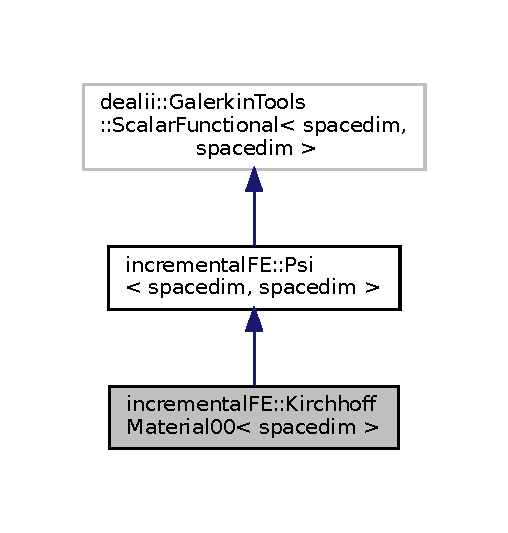
\includegraphics[width=229pt]{classincremental_f_e_1_1_kirchhoff_material00__inherit__graph}
\end{center}
\end{figure}


Collaboration diagram for incremental\+FE\+:\+:Kirchhoff\+Material00$<$ spacedim $>$\+:\nopagebreak
\begin{figure}[H]
\begin{center}
\leavevmode
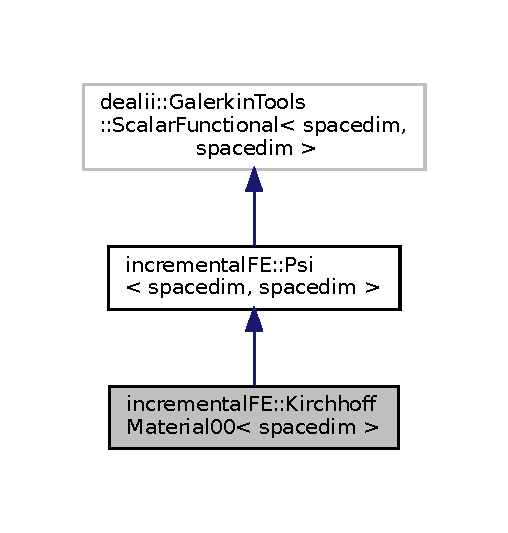
\includegraphics[width=229pt]{classincremental_f_e_1_1_kirchhoff_material00__coll__graph}
\end{center}
\end{figure}
\subsection*{Public Member Functions}
\begin{DoxyCompactItemize}
\item 
\hyperlink{classincremental_f_e_1_1_kirchhoff_material00_aed371b8af0803cbfb69989f78f99d6d0}{Kirchhoff\+Material00} (const std\+::vector$<$ dealii\+::\+Galerkin\+Tools\+::\+Dependent\+Field$<$ spacedim, spacedim $>$$>$ e\+\_\+omega, const std\+::set$<$ {\bf dealii\+::types\+::material\+\_\+id} $>$ domain\+\_\+of\+\_\+integration, const dealii\+::\+Quadrature$<$ spacedim $>$ quadrature, \hyperlink{classincremental_f_e_1_1_global_data_incremental_f_e}{Global\+Data\+Incremental\+FE}$<$ spacedim $>$ \&\hyperlink{classincremental_f_e_1_1_psi_3_01spacedim_00_01spacedim_01_4_abf0a4804877fd7cc9bd1b90e52760ba9}{global\+\_\+data}, const double \hyperlink{classincremental_f_e_1_1_kirchhoff_material00_a7dad9ce289d7ebe9363b82a2fd850067}{lambda}, const double \hyperlink{classincremental_f_e_1_1_kirchhoff_material00_a27770f7ae063508ca40aa009925c4a0b}{mu}, const double \hyperlink{classincremental_f_e_1_1_kirchhoff_material00_ae3992c464bbc9e18a3fc59ffec0b7bc3}{deps}, const double \hyperlink{classincremental_f_e_1_1_kirchhoff_material00_a4471a11a192ede0c9b16ea8ac9a35c4d}{c\+\_\+ref}, const double \hyperlink{classincremental_f_e_1_1_psi_3_01spacedim_00_01spacedim_01_4_af7b8227188dbdd6ada35b9445d96c79d}{alpha})
\item 
bool \hyperlink{classincremental_f_e_1_1_kirchhoff_material00_a5a8beb79b5b3758705bf75fe976f6cac}{get\+\_\+values\+\_\+and\+\_\+derivatives} (const {\bf dealii\+::\+Vector}$<$ double $>$ \&{\bf values}, const dealii\+::\+Point$<$ spacedim $>$ \&, double \&omega, {\bf dealii\+::\+Vector}$<$ double $>$ \&d\+\_\+omega, dealii\+::\+Full\+Matrix$<$ double $>$ \&d2\+\_\+omega, const std\+::tuple$<$ bool, bool, bool $>$ requested\+\_\+quantities) const 
\end{DoxyCompactItemize}
\subsection*{Private Attributes}
\begin{DoxyCompactItemize}
\item 
const double \hyperlink{classincremental_f_e_1_1_kirchhoff_material00_a7dad9ce289d7ebe9363b82a2fd850067}{lambda}
\item 
const double \hyperlink{classincremental_f_e_1_1_kirchhoff_material00_a27770f7ae063508ca40aa009925c4a0b}{mu}
\item 
const double \hyperlink{classincremental_f_e_1_1_kirchhoff_material00_ae3992c464bbc9e18a3fc59ffec0b7bc3}{deps}
\item 
const double \hyperlink{classincremental_f_e_1_1_kirchhoff_material00_a4471a11a192ede0c9b16ea8ac9a35c4d}{c\+\_\+ref}
\end{DoxyCompactItemize}


\subsection{Detailed Description}
\subsubsection*{template$<$unsigned int spacedim$>$\\*
class incremental\+F\+E\+::\+Kirchhoff\+Material00$<$ spacedim $>$}

Class defining a domain related scalar functional with the integrand

$h^\Omega_\rho = \dfrac{\lambda}{2} \left[\mathrm{tr}\left(\boldsymbol{E}^\mathrm{e}\right)\right]^2 + \mu\mathrm{tr}\left[\left(\boldsymbol{E}^\mathrm{e}\right)^2\right]$,

where

$ \boldsymbol{E}^\mathrm{e} = \boldsymbol{E} - \dfrac{\Delta \varepsilon}{3} \left( \dfrac{c}{c^{\mathrm{ref}}} - 1 \right) \mathbf{I} $

and

$ \boldsymbol{E} = \dfrac{1}{2} ( \boldsymbol{F}^\top \cdot \boldsymbol{F} - \boldsymbol{I} ) $

Here, $\boldsymbol{F}$ is the deformation gradient, $c$ is a species concentration, $\lambda$ and $\mu$ are Lame\textquotesingle{}s constants, $\Delta \varepsilon$ describes the magnitude of the isotropic stress free strain related to a change in $c$, and $c^{\mathrm{ref}}$ is the species concentration at which the stress free strain is zero.

The relation represents a Saint Venant -\/ Kirchhoff material with additional isotropic volumetric strain.

Ordering of quantities in {\bf Scalar\+Functional$<$spacedim, spacedim$>$\+::e\+\_\+omega} \+:~\newline
 \mbox{[}0\mbox{]} $F_{xx}$ ~\newline
 \mbox{[}1\mbox{]} $F_{xy}$ ~\newline
 \mbox{[}2\mbox{]} $F_{xz}$ ~\newline
 \mbox{[}3\mbox{]} $F_{yx}$ ~\newline
 \mbox{[}4\mbox{]} $F_{yy}$ ~\newline
 \mbox{[}5\mbox{]} $F_{yz}$ ~\newline
 \mbox{[}6\mbox{]} $F_{zx}$ ~\newline
 \mbox{[}7\mbox{]} $F_{zy}$ ~\newline
 \mbox{[}8\mbox{]} $F_{zz}$ ~\newline
 \mbox{[}9\mbox{]} $c$ 

\subsection{Constructor \& Destructor Documentation}
\index{incremental\+F\+E\+::\+Kirchhoff\+Material00@{incremental\+F\+E\+::\+Kirchhoff\+Material00}!Kirchhoff\+Material00@{Kirchhoff\+Material00}}
\index{Kirchhoff\+Material00@{Kirchhoff\+Material00}!incremental\+F\+E\+::\+Kirchhoff\+Material00@{incremental\+F\+E\+::\+Kirchhoff\+Material00}}
\subsubsection[{\texorpdfstring{Kirchhoff\+Material00(const std\+::vector$<$ dealii\+::\+Galerkin\+Tools\+::\+Dependent\+Field$<$ spacedim, spacedim $>$$>$ e\+\_\+omega, const std\+::set$<$ dealii\+::types\+::material\+\_\+id $>$ domain\+\_\+of\+\_\+integration, const dealii\+::\+Quadrature$<$ spacedim $>$ quadrature, Global\+Data\+Incremental\+F\+E$<$ spacedim $>$ \&global\+\_\+data, const double lambda, const double mu, const double deps, const double c\+\_\+ref, const double alpha)}{KirchhoffMaterial00(const std::vector< dealii::GalerkinTools::DependentField< spacedim, spacedim >> e_omega, const std::set< dealii::types::material_id > domain_of_integration, const dealii::Quadrature< spacedim > quadrature, GlobalDataIncrementalFE< spacedim > &global_data, const double lambda, const double mu, const double deps, const double c_ref, const double alpha)}}]{\setlength{\rightskip}{0pt plus 5cm}template$<$unsigned int spacedim$>$ {\bf incremental\+F\+E\+::\+Kirchhoff\+Material00}$<$ spacedim $>$\+::{\bf Kirchhoff\+Material00} (
\begin{DoxyParamCaption}
\item[{const std\+::vector$<$ dealii\+::\+Galerkin\+Tools\+::\+Dependent\+Field$<$ spacedim, spacedim $>$$>$}]{e\+\_\+omega, }
\item[{const std\+::set$<$ {\bf dealii\+::types\+::material\+\_\+id} $>$}]{domain\+\_\+of\+\_\+integration, }
\item[{const dealii\+::\+Quadrature$<$ spacedim $>$}]{quadrature, }
\item[{{\bf Global\+Data\+Incremental\+FE}$<$ spacedim $>$ \&}]{global\+\_\+data, }
\item[{const double}]{lambda, }
\item[{const double}]{mu, }
\item[{const double}]{deps, }
\item[{const double}]{c\+\_\+ref, }
\item[{const double}]{alpha}
\end{DoxyParamCaption}
)\hspace{0.3cm}{\ttfamily [inline]}}\hypertarget{classincremental_f_e_1_1_kirchhoff_material00_aed371b8af0803cbfb69989f78f99d6d0}{}\label{classincremental_f_e_1_1_kirchhoff_material00_aed371b8af0803cbfb69989f78f99d6d0}
Constructor


\begin{DoxyParams}[1]{Parameters}
\mbox{\tt in}  & {\em e\+\_\+omega} & {\bf Scalar\+Functional$<$spacedim, spacedim$>$\+::e\+\_\+omega}\\
\hline
\mbox{\tt in}  & {\em domain\+\_\+of\+\_\+integration} & {\bf Scalar\+Functional$<$spacedim, spacedim$>$\+::domain\+\_\+of\+\_\+integration}\\
\hline
\mbox{\tt in}  & {\em quadrature} & {\bf Scalar\+Functional$<$spacedim, spacedim$>$\+::quadrature}\\
\hline
\mbox{\tt in}  & {\em global\+\_\+data} & \hyperlink{classincremental_f_e_1_1_psi_3_01spacedim_00_01spacedim_01_4_abf0a4804877fd7cc9bd1b90e52760ba9}{Psi$<$spacedim, spacedim$>$\+::global\+\_\+data}\\
\hline
\mbox{\tt in}  & {\em lambda} & \hyperlink{classincremental_f_e_1_1_kirchhoff_material00_a7dad9ce289d7ebe9363b82a2fd850067}{Kirchhoff\+Material00\+::lambda}\\
\hline
\mbox{\tt in}  & {\em mu} & \hyperlink{classincremental_f_e_1_1_kirchhoff_material00_a27770f7ae063508ca40aa009925c4a0b}{Kirchhoff\+Material00\+::mu}\\
\hline
\mbox{\tt in}  & {\em deps} & \hyperlink{classincremental_f_e_1_1_kirchhoff_material00_ae3992c464bbc9e18a3fc59ffec0b7bc3}{Kirchhoff\+Material00\+::deps}\\
\hline
\mbox{\tt in}  & {\em c\+\_\+ref} & \hyperlink{classincremental_f_e_1_1_kirchhoff_material00_a4471a11a192ede0c9b16ea8ac9a35c4d}{Kirchhoff\+Material00\+::c\+\_\+ref}\\
\hline
\mbox{\tt in}  & {\em alpha} & \hyperlink{classincremental_f_e_1_1_psi_3_01spacedim_00_01spacedim_01_4_af7b8227188dbdd6ada35b9445d96c79d}{Psi$<$spacedim, spacedim$>$\+::alpha} \\
\hline
\end{DoxyParams}


\subsection{Member Function Documentation}
\index{incremental\+F\+E\+::\+Kirchhoff\+Material00@{incremental\+F\+E\+::\+Kirchhoff\+Material00}!get\+\_\+values\+\_\+and\+\_\+derivatives@{get\+\_\+values\+\_\+and\+\_\+derivatives}}
\index{get\+\_\+values\+\_\+and\+\_\+derivatives@{get\+\_\+values\+\_\+and\+\_\+derivatives}!incremental\+F\+E\+::\+Kirchhoff\+Material00@{incremental\+F\+E\+::\+Kirchhoff\+Material00}}
\subsubsection[{\texorpdfstring{get\+\_\+values\+\_\+and\+\_\+derivatives(const dealii\+::\+Vector$<$ double $>$ \&values, const dealii\+::\+Point$<$ spacedim $>$ \&, double \&omega, dealii\+::\+Vector$<$ double $>$ \&d\+\_\+omega, dealii\+::\+Full\+Matrix$<$ double $>$ \&d2\+\_\+omega, const std\+::tuple$<$ bool, bool, bool $>$ requested\+\_\+quantities) const }{get_values_and_derivatives(const dealii::Vector< double > &values, const dealii::Point< spacedim > &, double &omega, dealii::Vector< double > &d_omega, dealii::FullMatrix< double > &d2_omega, const std::tuple< bool, bool, bool > requested_quantities) const }}]{\setlength{\rightskip}{0pt plus 5cm}template$<$unsigned int spacedim$>$ bool {\bf incremental\+F\+E\+::\+Kirchhoff\+Material00}$<$ spacedim $>$\+::get\+\_\+values\+\_\+and\+\_\+derivatives (
\begin{DoxyParamCaption}
\item[{const {\bf dealii\+::\+Vector}$<$ double $>$ \&}]{values, }
\item[{const dealii\+::\+Point$<$ spacedim $>$ \&}]{, }
\item[{double \&}]{omega, }
\item[{{\bf dealii\+::\+Vector}$<$ double $>$ \&}]{d\+\_\+omega, }
\item[{dealii\+::\+Full\+Matrix$<$ double $>$ \&}]{d2\+\_\+omega, }
\item[{const std\+::tuple$<$ bool, bool, bool $>$}]{requested\+\_\+quantities}
\end{DoxyParamCaption}
) const\hspace{0.3cm}{\ttfamily [inline]}, {\ttfamily [virtual]}}\hypertarget{classincremental_f_e_1_1_kirchhoff_material00_a5a8beb79b5b3758705bf75fe976f6cac}{}\label{classincremental_f_e_1_1_kirchhoff_material00_a5a8beb79b5b3758705bf75fe976f6cac}
\begin{DoxySeeAlso}{See also}
\hyperlink{classincremental_f_e_1_1_psi_3_01spacedim_00_01spacedim_01_4_a17f3559c196edb5487b591bb6061667e}{Psi$<$spacedim, spacedim$>$\+::get\+\_\+values\+\_\+and\+\_\+derivatives()} 
\end{DoxySeeAlso}


Implements \hyperlink{classincremental_f_e_1_1_psi_3_01spacedim_00_01spacedim_01_4_a17f3559c196edb5487b591bb6061667e}{incremental\+F\+E\+::\+Psi$<$ spacedim, spacedim $>$}.



\subsection{Member Data Documentation}
\index{incremental\+F\+E\+::\+Kirchhoff\+Material00@{incremental\+F\+E\+::\+Kirchhoff\+Material00}!c\+\_\+ref@{c\+\_\+ref}}
\index{c\+\_\+ref@{c\+\_\+ref}!incremental\+F\+E\+::\+Kirchhoff\+Material00@{incremental\+F\+E\+::\+Kirchhoff\+Material00}}
\subsubsection[{\texorpdfstring{c\+\_\+ref}{c_ref}}]{\setlength{\rightskip}{0pt plus 5cm}template$<$unsigned int spacedim$>$ const double {\bf incremental\+F\+E\+::\+Kirchhoff\+Material00}$<$ spacedim $>$\+::c\+\_\+ref\hspace{0.3cm}{\ttfamily [private]}}\hypertarget{classincremental_f_e_1_1_kirchhoff_material00_a4471a11a192ede0c9b16ea8ac9a35c4d}{}\label{classincremental_f_e_1_1_kirchhoff_material00_a4471a11a192ede0c9b16ea8ac9a35c4d}
$c^\mathrm{ref}$ \index{incremental\+F\+E\+::\+Kirchhoff\+Material00@{incremental\+F\+E\+::\+Kirchhoff\+Material00}!deps@{deps}}
\index{deps@{deps}!incremental\+F\+E\+::\+Kirchhoff\+Material00@{incremental\+F\+E\+::\+Kirchhoff\+Material00}}
\subsubsection[{\texorpdfstring{deps}{deps}}]{\setlength{\rightskip}{0pt plus 5cm}template$<$unsigned int spacedim$>$ const double {\bf incremental\+F\+E\+::\+Kirchhoff\+Material00}$<$ spacedim $>$\+::deps\hspace{0.3cm}{\ttfamily [private]}}\hypertarget{classincremental_f_e_1_1_kirchhoff_material00_ae3992c464bbc9e18a3fc59ffec0b7bc3}{}\label{classincremental_f_e_1_1_kirchhoff_material00_ae3992c464bbc9e18a3fc59ffec0b7bc3}
$\Delta \varepsilon$ \index{incremental\+F\+E\+::\+Kirchhoff\+Material00@{incremental\+F\+E\+::\+Kirchhoff\+Material00}!lambda@{lambda}}
\index{lambda@{lambda}!incremental\+F\+E\+::\+Kirchhoff\+Material00@{incremental\+F\+E\+::\+Kirchhoff\+Material00}}
\subsubsection[{\texorpdfstring{lambda}{lambda}}]{\setlength{\rightskip}{0pt plus 5cm}template$<$unsigned int spacedim$>$ const double {\bf incremental\+F\+E\+::\+Kirchhoff\+Material00}$<$ spacedim $>$\+::lambda\hspace{0.3cm}{\ttfamily [private]}}\hypertarget{classincremental_f_e_1_1_kirchhoff_material00_a7dad9ce289d7ebe9363b82a2fd850067}{}\label{classincremental_f_e_1_1_kirchhoff_material00_a7dad9ce289d7ebe9363b82a2fd850067}
Lame\textquotesingle{}s constant $\lambda$ \index{incremental\+F\+E\+::\+Kirchhoff\+Material00@{incremental\+F\+E\+::\+Kirchhoff\+Material00}!mu@{mu}}
\index{mu@{mu}!incremental\+F\+E\+::\+Kirchhoff\+Material00@{incremental\+F\+E\+::\+Kirchhoff\+Material00}}
\subsubsection[{\texorpdfstring{mu}{mu}}]{\setlength{\rightskip}{0pt plus 5cm}template$<$unsigned int spacedim$>$ const double {\bf incremental\+F\+E\+::\+Kirchhoff\+Material00}$<$ spacedim $>$\+::mu\hspace{0.3cm}{\ttfamily [private]}}\hypertarget{classincremental_f_e_1_1_kirchhoff_material00_a27770f7ae063508ca40aa009925c4a0b}{}\label{classincremental_f_e_1_1_kirchhoff_material00_a27770f7ae063508ca40aa009925c4a0b}
Lame\textquotesingle{}s constant $\lambda$ 

The documentation for this class was generated from the following file\+:\begin{DoxyCompactItemize}
\item 
/home/sst/code/\+Incremental\+F\+E/\+Incremental\+F\+E/include/incremental\+\_\+fe/scalar\+\_\+functionals/\hyperlink{psi__lib_8h}{psi\+\_\+lib.\+h}\end{DoxyCompactItemize}

\hypertarget{classincremental_f_e_1_1_neo_hooke_compression_point00}{}\doxysection{incremental\+FE\+::Neo\+Hooke\+Compression\+Point00$<$ spacedim $>$ Class Template Reference}
\label{classincremental_f_e_1_1_neo_hooke_compression_point00}\index{incrementalFE::NeoHookeCompressionPoint00$<$ spacedim $>$@{incrementalFE::NeoHookeCompressionPoint00$<$ spacedim $>$}}


{\ttfamily \#include $<$psi\+\_\+lib.\+h$>$}



Inheritance diagram for incremental\+FE\+::Neo\+Hooke\+Compression\+Point00$<$ spacedim $>$\+:\nopagebreak
\begin{figure}[H]
\begin{center}
\leavevmode
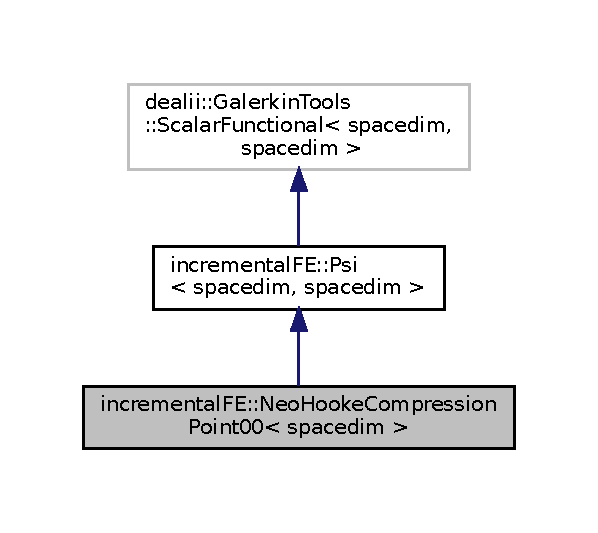
\includegraphics[width=287pt]{classincremental_f_e_1_1_neo_hooke_compression_point00__inherit__graph}
\end{center}
\end{figure}


Collaboration diagram for incremental\+FE\+::Neo\+Hooke\+Compression\+Point00$<$ spacedim $>$\+:\nopagebreak
\begin{figure}[H]
\begin{center}
\leavevmode
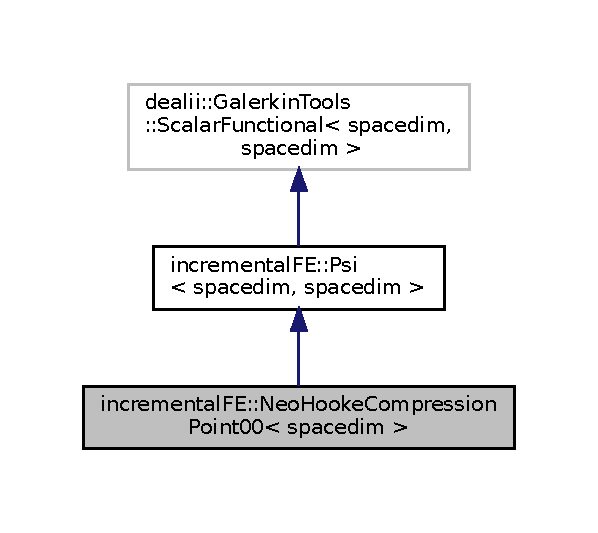
\includegraphics[width=287pt]{classincremental_f_e_1_1_neo_hooke_compression_point00__coll__graph}
\end{center}
\end{figure}
\doxysubsection*{Public Member Functions}
\begin{DoxyCompactItemize}
\item 
\mbox{\hyperlink{classincremental_f_e_1_1_neo_hooke_compression_point00_a8ebddd648a42cf4ff992b8e2db221f42}{Neo\+Hooke\+Compression\+Point00}} (const std\+::vector$<$ dealii\+::\+Galerkin\+Tools\+::\+Dependent\+Field$<$ spacedim, spacedim $>$$>$ e\+\_\+omega, const std\+::set$<$ \textbf{ dealii\+::types\+::material\+\_\+id} $>$ domain\+\_\+of\+\_\+integration, const dealii\+::\+Quadrature$<$ spacedim $>$ quadrature, \mbox{\hyperlink{classincremental_f_e_1_1_global_data_incremental_f_e}{Global\+Data\+Incremental\+FE}}$<$ spacedim $>$ \&\mbox{\hyperlink{classincremental_f_e_1_1_psi_3_01spacedim_00_01spacedim_01_4_abf0a4804877fd7cc9bd1b90e52760ba9}{global\+\_\+data}}, const double \mbox{\hyperlink{classincremental_f_e_1_1_neo_hooke_compression_point00_a1b1c0c8dcca2410288a9ef014a117870}{lambda}}, const double \mbox{\hyperlink{classincremental_f_e_1_1_neo_hooke_compression_point00_a647e6e22708201ca6093e1daeaf7326c}{mu}}, const double \mbox{\hyperlink{classincremental_f_e_1_1_neo_hooke_compression_point00_aba531cf944d6455c9aebc49bdcb45019}{n\+\_\+0}}, const double \mbox{\hyperlink{classincremental_f_e_1_1_psi_3_01spacedim_00_01spacedim_01_4_aaeb0d41ffa60afde6010e30270d47801}{alpha}})
\item 
bool \mbox{\hyperlink{classincremental_f_e_1_1_neo_hooke_compression_point00_ab062fe5ffbea799d817b3106d15cefc3}{get\+\_\+values\+\_\+and\+\_\+derivatives}} (const \textbf{ dealii\+::\+Vector}$<$ double $>$ \&\textbf{ values}, const dealii\+::\+Point$<$ spacedim $>$ \&, double \&omega, \textbf{ dealii\+::\+Vector}$<$ double $>$ \&d\+\_\+omega, dealii\+::\+Full\+Matrix$<$ double $>$ \&d2\+\_\+omega, const std\+::tuple$<$ bool, bool, bool $>$ requested\+\_\+quantities) const
\item 
double \mbox{\hyperlink{classincremental_f_e_1_1_neo_hooke_compression_point00_a73ace9c77416b4734f5c7babc0c1ad12}{get\+\_\+maximum\+\_\+step}} (const \textbf{ dealii\+::\+Vector}$<$ double $>$ \&e\+\_\+omega, const std\+::vector$<$ \textbf{ dealii\+::\+Vector}$<$ double $>$$>$ \&, const \textbf{ dealii\+::\+Vector}$<$ double $>$ \&delta\+\_\+e\+\_\+omega, const \textbf{ dealii\+::\+Vector}$<$ double $>$ \&, const dealii\+::\+Point$<$ spacedim $>$ \&) const
\end{DoxyCompactItemize}
\doxysubsection*{Private Attributes}
\begin{DoxyCompactItemize}
\item 
const double \mbox{\hyperlink{classincremental_f_e_1_1_neo_hooke_compression_point00_a1b1c0c8dcca2410288a9ef014a117870}{lambda}}
\item 
const double \mbox{\hyperlink{classincremental_f_e_1_1_neo_hooke_compression_point00_a647e6e22708201ca6093e1daeaf7326c}{mu}}
\item 
const double \mbox{\hyperlink{classincremental_f_e_1_1_neo_hooke_compression_point00_aba531cf944d6455c9aebc49bdcb45019}{n\+\_\+0}}
\end{DoxyCompactItemize}
\doxysubsection*{Additional Inherited Members}


\doxysubsection{Detailed Description}
\subsubsection*{template$<$unsigned int spacedim$>$\newline
class incremental\+F\+E\+::\+Neo\+Hooke\+Compression\+Point00$<$ spacedim $>$}

Class defining Neo-\/\+Hooke material with \char`\"{}compression point\char`\"{} for hydrogel modeling. See PhD thesis Acartürk (2009)\+: Simulation of Charged Hydrated Porous Materials, Eq. (3.\+99)

The integrand is

$h^\Omega_\rho = \dfrac{\mu}{2} ( \mathrm{tr}\boldsymbol{C} - 3 ) - \mu \mathrm{ln}J + \lambda (1-n_0)^2 \left( \dfrac{J-1}{1-n_0} - \mathrm{ln}\dfrac{J-n_0}{1-n_0} \right) $,

where

$ \boldsymbol{C} =\boldsymbol{F}^\top \cdot \boldsymbol{F} $ is the right Cauchy-\/\+Green deformation tensor, $J$ the determinant of the deformation gradient $\boldsymbol{F}$, $n_0$ the initial volume fraction of the polymeric backbone, and $\mu$ and $\lambda$ Lame\textquotesingle{}s constants.

Ordering of quantities in \textbf{ Scalar\+Functional$<$spacedim, spacedim$>$\+::e\+\_\+omega} \+:~\newline
 \mbox{[}0\mbox{]} $F_{xx}$ ~\newline
 \mbox{[}1\mbox{]} $F_{xy}$ ~\newline
 \mbox{[}2\mbox{]} $F_{xz}$ ~\newline
 \mbox{[}3\mbox{]} $F_{yx}$ ~\newline
 \mbox{[}4\mbox{]} $F_{yy}$ ~\newline
 \mbox{[}5\mbox{]} $F_{yz}$ ~\newline
 \mbox{[}6\mbox{]} $F_{zx}$ ~\newline
 \mbox{[}7\mbox{]} $F_{zy}$ ~\newline
 \mbox{[}8\mbox{]} $F_{zz}$ ~\newline
 

\doxysubsection{Constructor \& Destructor Documentation}
\mbox{\Hypertarget{classincremental_f_e_1_1_neo_hooke_compression_point00_a8ebddd648a42cf4ff992b8e2db221f42}\label{classincremental_f_e_1_1_neo_hooke_compression_point00_a8ebddd648a42cf4ff992b8e2db221f42}} 
\index{incrementalFE::NeoHookeCompressionPoint00$<$ spacedim $>$@{incrementalFE::NeoHookeCompressionPoint00$<$ spacedim $>$}!NeoHookeCompressionPoint00@{NeoHookeCompressionPoint00}}
\index{NeoHookeCompressionPoint00@{NeoHookeCompressionPoint00}!incrementalFE::NeoHookeCompressionPoint00$<$ spacedim $>$@{incrementalFE::NeoHookeCompressionPoint00$<$ spacedim $>$}}
\doxysubsubsection{\texorpdfstring{NeoHookeCompressionPoint00()}{NeoHookeCompressionPoint00()}}
{\footnotesize\ttfamily template$<$unsigned int spacedim$>$ \\
\mbox{\hyperlink{classincremental_f_e_1_1_neo_hooke_compression_point00}{incremental\+F\+E\+::\+Neo\+Hooke\+Compression\+Point00}}$<$ spacedim $>$\+::\mbox{\hyperlink{classincremental_f_e_1_1_neo_hooke_compression_point00}{Neo\+Hooke\+Compression\+Point00}} (\begin{DoxyParamCaption}\item[{const std\+::vector$<$ dealii\+::\+Galerkin\+Tools\+::\+Dependent\+Field$<$ spacedim, spacedim $>$$>$}]{e\+\_\+omega,  }\item[{const std\+::set$<$ \textbf{ dealii\+::types\+::material\+\_\+id} $>$}]{domain\+\_\+of\+\_\+integration,  }\item[{const dealii\+::\+Quadrature$<$ spacedim $>$}]{quadrature,  }\item[{\mbox{\hyperlink{classincremental_f_e_1_1_global_data_incremental_f_e}{Global\+Data\+Incremental\+FE}}$<$ spacedim $>$ \&}]{global\+\_\+data,  }\item[{const double}]{lambda,  }\item[{const double}]{mu,  }\item[{const double}]{n\+\_\+0,  }\item[{const double}]{alpha }\end{DoxyParamCaption})\hspace{0.3cm}{\ttfamily [inline]}}

Constructor


\begin{DoxyParams}[1]{Parameters}
\mbox{\texttt{ in}}  & {\em e\+\_\+omega} & \textbf{ Scalar\+Functional$<$spacedim, spacedim$>$\+::e\+\_\+omega}\\
\hline
\mbox{\texttt{ in}}  & {\em domain\+\_\+of\+\_\+integration} & \textbf{ Scalar\+Functional$<$spacedim, spacedim$>$\+::domain\+\_\+of\+\_\+integration}\\
\hline
\mbox{\texttt{ in}}  & {\em quadrature} & \textbf{ Scalar\+Functional$<$spacedim, spacedim$>$\+::quadrature}\\
\hline
\mbox{\texttt{ in}}  & {\em global\+\_\+data} & \mbox{\hyperlink{classincremental_f_e_1_1_psi_3_01spacedim_00_01spacedim_01_4_abf0a4804877fd7cc9bd1b90e52760ba9}{Psi$<$spacedim, spacedim$>$\+::global\+\_\+data}}\\
\hline
\mbox{\texttt{ in}}  & {\em lambda} & \mbox{\hyperlink{classincremental_f_e_1_1_neo_hooke_compression_point00_a1b1c0c8dcca2410288a9ef014a117870}{Neo\+Hooke\+Compression\+Point00\+::lambda}}\\
\hline
\mbox{\texttt{ in}}  & {\em mu} & \mbox{\hyperlink{classincremental_f_e_1_1_neo_hooke_compression_point00_a647e6e22708201ca6093e1daeaf7326c}{Neo\+Hooke\+Compression\+Point00\+::mu}}\\
\hline
\mbox{\texttt{ in}}  & {\em n\+\_\+0} & \mbox{\hyperlink{classincremental_f_e_1_1_neo_hooke_compression_point00_aba531cf944d6455c9aebc49bdcb45019}{Neo\+Hooke\+Compression\+Point00\+::n\+\_\+0}}\\
\hline
\mbox{\texttt{ in}}  & {\em alpha} & \mbox{\hyperlink{classincremental_f_e_1_1_psi_3_01spacedim_00_01spacedim_01_4_aaeb0d41ffa60afde6010e30270d47801}{Psi$<$spacedim, spacedim$>$\+::alpha}} \\
\hline
\end{DoxyParams}


\doxysubsection{Member Function Documentation}
\mbox{\Hypertarget{classincremental_f_e_1_1_neo_hooke_compression_point00_a73ace9c77416b4734f5c7babc0c1ad12}\label{classincremental_f_e_1_1_neo_hooke_compression_point00_a73ace9c77416b4734f5c7babc0c1ad12}} 
\index{incrementalFE::NeoHookeCompressionPoint00$<$ spacedim $>$@{incrementalFE::NeoHookeCompressionPoint00$<$ spacedim $>$}!get\_maximum\_step@{get\_maximum\_step}}
\index{get\_maximum\_step@{get\_maximum\_step}!incrementalFE::NeoHookeCompressionPoint00$<$ spacedim $>$@{incrementalFE::NeoHookeCompressionPoint00$<$ spacedim $>$}}
\doxysubsubsection{\texorpdfstring{get\_maximum\_step()}{get\_maximum\_step()}}
{\footnotesize\ttfamily template$<$unsigned int spacedim$>$ \\
double \mbox{\hyperlink{classincremental_f_e_1_1_neo_hooke_compression_point00}{incremental\+F\+E\+::\+Neo\+Hooke\+Compression\+Point00}}$<$ spacedim $>$\+::get\+\_\+maximum\+\_\+step (\begin{DoxyParamCaption}\item[{const \textbf{ dealii\+::\+Vector}$<$ double $>$ \&}]{e\+\_\+omega,  }\item[{const std\+::vector$<$ \textbf{ dealii\+::\+Vector}$<$ double $>$$>$ \&}]{,  }\item[{const \textbf{ dealii\+::\+Vector}$<$ double $>$ \&}]{delta\+\_\+e\+\_\+omega,  }\item[{const \textbf{ dealii\+::\+Vector}$<$ double $>$ \&}]{,  }\item[{const dealii\+::\+Point$<$ spacedim $>$ \&}]{ }\end{DoxyParamCaption}) const\hspace{0.3cm}{\ttfamily [inline]}}

see \textbf{ Scalar\+Functional$<$spacedim, spacedim$>$\+::get\+\_\+maximum\+\_\+step} \mbox{\Hypertarget{classincremental_f_e_1_1_neo_hooke_compression_point00_ab062fe5ffbea799d817b3106d15cefc3}\label{classincremental_f_e_1_1_neo_hooke_compression_point00_ab062fe5ffbea799d817b3106d15cefc3}} 
\index{incrementalFE::NeoHookeCompressionPoint00$<$ spacedim $>$@{incrementalFE::NeoHookeCompressionPoint00$<$ spacedim $>$}!get\_values\_and\_derivatives@{get\_values\_and\_derivatives}}
\index{get\_values\_and\_derivatives@{get\_values\_and\_derivatives}!incrementalFE::NeoHookeCompressionPoint00$<$ spacedim $>$@{incrementalFE::NeoHookeCompressionPoint00$<$ spacedim $>$}}
\doxysubsubsection{\texorpdfstring{get\_values\_and\_derivatives()}{get\_values\_and\_derivatives()}}
{\footnotesize\ttfamily template$<$unsigned int spacedim$>$ \\
bool \mbox{\hyperlink{classincremental_f_e_1_1_neo_hooke_compression_point00}{incremental\+F\+E\+::\+Neo\+Hooke\+Compression\+Point00}}$<$ spacedim $>$\+::get\+\_\+values\+\_\+and\+\_\+derivatives (\begin{DoxyParamCaption}\item[{const \textbf{ dealii\+::\+Vector}$<$ double $>$ \&}]{values,  }\item[{const dealii\+::\+Point$<$ spacedim $>$ \&}]{,  }\item[{double \&}]{omega,  }\item[{\textbf{ dealii\+::\+Vector}$<$ double $>$ \&}]{d\+\_\+omega,  }\item[{dealii\+::\+Full\+Matrix$<$ double $>$ \&}]{d2\+\_\+omega,  }\item[{const std\+::tuple$<$ bool, bool, bool $>$}]{requested\+\_\+quantities }\end{DoxyParamCaption}) const\hspace{0.3cm}{\ttfamily [inline]}, {\ttfamily [virtual]}}

\begin{DoxySeeAlso}{See also}
\mbox{\hyperlink{classincremental_f_e_1_1_psi_3_01spacedim_00_01spacedim_01_4_a17f3559c196edb5487b591bb6061667e}{Psi$<$spacedim, spacedim$>$\+::get\+\_\+values\+\_\+and\+\_\+derivatives()}} 
\end{DoxySeeAlso}


Implements \mbox{\hyperlink{classincremental_f_e_1_1_psi_3_01spacedim_00_01spacedim_01_4_a17f3559c196edb5487b591bb6061667e}{incremental\+F\+E\+::\+Psi$<$ spacedim, spacedim $>$}}.



\doxysubsection{Member Data Documentation}
\mbox{\Hypertarget{classincremental_f_e_1_1_neo_hooke_compression_point00_a1b1c0c8dcca2410288a9ef014a117870}\label{classincremental_f_e_1_1_neo_hooke_compression_point00_a1b1c0c8dcca2410288a9ef014a117870}} 
\index{incrementalFE::NeoHookeCompressionPoint00$<$ spacedim $>$@{incrementalFE::NeoHookeCompressionPoint00$<$ spacedim $>$}!lambda@{lambda}}
\index{lambda@{lambda}!incrementalFE::NeoHookeCompressionPoint00$<$ spacedim $>$@{incrementalFE::NeoHookeCompressionPoint00$<$ spacedim $>$}}
\doxysubsubsection{\texorpdfstring{lambda}{lambda}}
{\footnotesize\ttfamily template$<$unsigned int spacedim$>$ \\
const double \mbox{\hyperlink{classincremental_f_e_1_1_neo_hooke_compression_point00}{incremental\+F\+E\+::\+Neo\+Hooke\+Compression\+Point00}}$<$ spacedim $>$\+::lambda\hspace{0.3cm}{\ttfamily [private]}}

Lame\textquotesingle{}s constant $\lambda$ \mbox{\Hypertarget{classincremental_f_e_1_1_neo_hooke_compression_point00_a647e6e22708201ca6093e1daeaf7326c}\label{classincremental_f_e_1_1_neo_hooke_compression_point00_a647e6e22708201ca6093e1daeaf7326c}} 
\index{incrementalFE::NeoHookeCompressionPoint00$<$ spacedim $>$@{incrementalFE::NeoHookeCompressionPoint00$<$ spacedim $>$}!mu@{mu}}
\index{mu@{mu}!incrementalFE::NeoHookeCompressionPoint00$<$ spacedim $>$@{incrementalFE::NeoHookeCompressionPoint00$<$ spacedim $>$}}
\doxysubsubsection{\texorpdfstring{mu}{mu}}
{\footnotesize\ttfamily template$<$unsigned int spacedim$>$ \\
const double \mbox{\hyperlink{classincremental_f_e_1_1_neo_hooke_compression_point00}{incremental\+F\+E\+::\+Neo\+Hooke\+Compression\+Point00}}$<$ spacedim $>$\+::mu\hspace{0.3cm}{\ttfamily [private]}}

Lame\textquotesingle{}s constant $\mu$ \mbox{\Hypertarget{classincremental_f_e_1_1_neo_hooke_compression_point00_aba531cf944d6455c9aebc49bdcb45019}\label{classincremental_f_e_1_1_neo_hooke_compression_point00_aba531cf944d6455c9aebc49bdcb45019}} 
\index{incrementalFE::NeoHookeCompressionPoint00$<$ spacedim $>$@{incrementalFE::NeoHookeCompressionPoint00$<$ spacedim $>$}!n\_0@{n\_0}}
\index{n\_0@{n\_0}!incrementalFE::NeoHookeCompressionPoint00$<$ spacedim $>$@{incrementalFE::NeoHookeCompressionPoint00$<$ spacedim $>$}}
\doxysubsubsection{\texorpdfstring{n\_0}{n\_0}}
{\footnotesize\ttfamily template$<$unsigned int spacedim$>$ \\
const double \mbox{\hyperlink{classincremental_f_e_1_1_neo_hooke_compression_point00}{incremental\+F\+E\+::\+Neo\+Hooke\+Compression\+Point00}}$<$ spacedim $>$\+::n\+\_\+0\hspace{0.3cm}{\ttfamily [private]}}

Initial volume fraction of polymeric backbone $n_0$ 

The documentation for this class was generated from the following file\+:\begin{DoxyCompactItemize}
\item 
/home/sst/code/\+Incremental\+F\+E/\+Incremental\+F\+E/include/incremental\+\_\+fe/scalar\+\_\+functionals/\mbox{\hyperlink{psi__lib_8h}{psi\+\_\+lib.\+h}}\end{DoxyCompactItemize}

\hypertarget{classincremental_f_e_1_1_omega}{}\doxysection{incremental\+FE\+::Omega$<$ dim, spacedim $>$ Class Template Reference}
\label{classincremental_f_e_1_1_omega}\index{incrementalFE::Omega$<$ dim, spacedim $>$@{incrementalFE::Omega$<$ dim, spacedim $>$}}


{\ttfamily \#include $<$omega.\+h$>$}



Inheritance diagram for incremental\+FE\+::Omega$<$ dim, spacedim $>$\+:\nopagebreak
\begin{figure}[H]
\begin{center}
\leavevmode
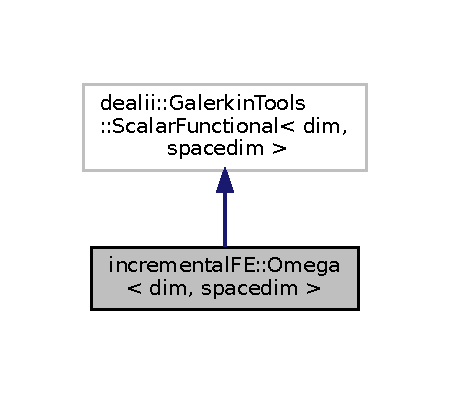
\includegraphics[width=216pt]{classincremental_f_e_1_1_omega__inherit__graph}
\end{center}
\end{figure}


Collaboration diagram for incremental\+FE\+::Omega$<$ dim, spacedim $>$\+:\nopagebreak
\begin{figure}[H]
\begin{center}
\leavevmode
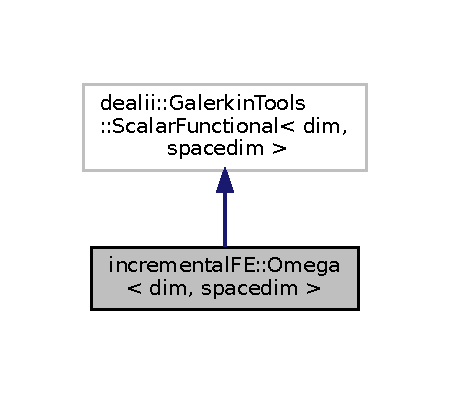
\includegraphics[width=216pt]{classincremental_f_e_1_1_omega__coll__graph}
\end{center}
\end{figure}
\doxysubsection*{Public Member Functions}
\begin{DoxyCompactItemize}
\item 
\mbox{\hyperlink{classincremental_f_e_1_1_omega_a53ca9e46c52887166cbb4f393d37f432}{Omega}} (const std\+::vector$<$ dealii\+::\+Galerkin\+Tools\+::\+Dependent\+Field$<$ dim, spacedim $>$$>$ e\+\_\+sigma, const std\+::set$<$ \textbf{ dealii\+::types\+::material\+\_\+id} $>$ domain\+\_\+of\+\_\+integration, const dealii\+::\+Quadrature$<$ dim $>$ quadrature, \mbox{\hyperlink{classincremental_f_e_1_1_global_data_incremental_f_e}{Global\+Data\+Incremental\+FE}}$<$ spacedim $>$ \&\mbox{\hyperlink{classincremental_f_e_1_1_omega_abd23d288a7a4a43f9b528be968cd2113}{global\+\_\+data}}, const unsigned int n\+\_\+v\+\_\+dot, const unsigned int n\+\_\+q\+\_\+dot, const unsigned int \mbox{\hyperlink{classincremental_f_e_1_1_omega_a322340b50451ab46f91cdcec95248f16}{n\+\_\+mu}}, const unsigned int \mbox{\hyperlink{classincremental_f_e_1_1_omega_addbf75c949792f6340ea40164a2bfee3}{n\+\_\+q}}, const unsigned int \mbox{\hyperlink{classincremental_f_e_1_1_omega_a7600d263ebf98129629e44fa67e8a58c}{method}}, const double \mbox{\hyperlink{classincremental_f_e_1_1_omega_a891688560ec0ad8dc5a0058a7b400269}{alpha}}=0.\+0, const std\+::string name=\char`\"{}Omega\char`\"{})
\item 
virtual \mbox{\hyperlink{classincremental_f_e_1_1_omega_a262968e5daadc162b22fdc58dd760976}{$\sim$\+Omega}} ()=default
\item 
virtual bool \mbox{\hyperlink{classincremental_f_e_1_1_omega_a2f35d862aefa11151de5b7c7411e45df}{get\+\_\+values\+\_\+and\+\_\+derivatives}} (const \textbf{ dealii\+::\+Vector}$<$ double $>$ \&\textbf{ values}, const double t, const dealii\+::\+Point$<$ spacedim $>$ \&x, const dealii\+::\+Tensor$<$ 1, spacedim $>$ \&n, double \&omega, \textbf{ dealii\+::\+Vector}$<$ double $>$ \&d\+\_\+omega, dealii\+::\+Full\+Matrix$<$ double $>$ \&d2\+\_\+omega, const std\+::tuple$<$ bool, bool, bool $>$ requested\+\_\+quantities, const bool compute\+\_\+d2q) const =0
\item 
bool \mbox{\hyperlink{classincremental_f_e_1_1_omega_a2faafa9ed88581fc3a4ff6967a8d64e7}{get\+\_\+h\+\_\+sigma}} (\textbf{ dealii\+::\+Vector}$<$ double $>$ \&e\+\_\+sigma, const std\+::vector$<$ \textbf{ dealii\+::\+Vector}$<$ double $>$$>$ \&e\+\_\+sigma\+\_\+ref\+\_\+sets, \textbf{ dealii\+::\+Vector}$<$ double $>$ \&hidden\+\_\+vars, const dealii\+::\+Point$<$ spacedim $>$ \&x, const dealii\+::\+Tensor$<$ 1, spacedim $>$ \&n, double \&h\+\_\+sigma, \textbf{ dealii\+::\+Vector}$<$ double $>$ \&h\+\_\+sigma\+\_\+1, dealii\+::\+Full\+Matrix$<$ double $>$ \&h\+\_\+sigma\+\_\+2, const std\+::tuple$<$ bool, bool, bool $>$ requested\+\_\+quantities) const final
\end{DoxyCompactItemize}
\doxysubsection*{Public Attributes}
\begin{DoxyCompactItemize}
\item 
const unsigned int \mbox{\hyperlink{classincremental_f_e_1_1_omega_a7fa938b26804b0dc15726f3423332880}{n\+\_\+v\+\_\+q\+\_\+dot}}
\item 
const unsigned int \mbox{\hyperlink{classincremental_f_e_1_1_omega_a322340b50451ab46f91cdcec95248f16}{n\+\_\+mu}}
\item 
const unsigned int \mbox{\hyperlink{classincremental_f_e_1_1_omega_addbf75c949792f6340ea40164a2bfee3}{n\+\_\+q}}
\item 
bool \mbox{\hyperlink{classincremental_f_e_1_1_omega_ac4bf419234cfacc3b7de36f39a36135a}{compute\+\_\+potential\+\_\+value}} = true
\end{DoxyCompactItemize}
\doxysubsection*{Private Attributes}
\begin{DoxyCompactItemize}
\item 
const dealii\+::\+Smart\+Pointer$<$ \mbox{\hyperlink{classincremental_f_e_1_1_global_data_incremental_f_e}{Global\+Data\+Incremental\+FE}}$<$ spacedim $>$ $>$ \mbox{\hyperlink{classincremental_f_e_1_1_omega_abd23d288a7a4a43f9b528be968cd2113}{global\+\_\+data}}
\item 
const double \mbox{\hyperlink{classincremental_f_e_1_1_omega_a891688560ec0ad8dc5a0058a7b400269}{alpha}}
\item 
const unsigned int \mbox{\hyperlink{classincremental_f_e_1_1_omega_a7600d263ebf98129629e44fa67e8a58c}{method}}
\end{DoxyCompactItemize}


\doxysubsection{Detailed Description}
\subsubsection*{template$<$unsigned int dim, unsigned int spacedim$>$\newline
class incremental\+F\+E\+::\+Omega$<$ dim, spacedim $>$}

Class defining the time discrete approximation of an interface related scalar functional with the integrand

$ \omega^\Sigma = \omega^\Sigma(\dot{v}, \dot{q}, \mu, q; t) $,

where $\dot{v}$, $\dot{q}$, $\mu$, and $q$ may be vectors.

The time discrete approximation is done either by Miehe\textquotesingle{}s method, by the $\alpha$-\/family, or by the modified $\alpha$-\/family. 

\doxysubsection{Constructor \& Destructor Documentation}
\mbox{\Hypertarget{classincremental_f_e_1_1_omega_a53ca9e46c52887166cbb4f393d37f432}\label{classincremental_f_e_1_1_omega_a53ca9e46c52887166cbb4f393d37f432}} 
\index{incrementalFE::Omega$<$ dim, spacedim $>$@{incrementalFE::Omega$<$ dim, spacedim $>$}!Omega@{Omega}}
\index{Omega@{Omega}!incrementalFE::Omega$<$ dim, spacedim $>$@{incrementalFE::Omega$<$ dim, spacedim $>$}}
\doxysubsubsection{\texorpdfstring{Omega()}{Omega()}}
{\footnotesize\ttfamily template$<$unsigned int dim, unsigned int spacedim$>$ \\
\mbox{\hyperlink{classincremental_f_e_1_1_omega}{incremental\+F\+E\+::\+Omega}}$<$ dim, spacedim $>$\+::\mbox{\hyperlink{classincremental_f_e_1_1_omega}{Omega}} (\begin{DoxyParamCaption}\item[{const std\+::vector$<$ dealii\+::\+Galerkin\+Tools\+::\+Dependent\+Field$<$ dim, spacedim $>$$>$}]{e\+\_\+sigma,  }\item[{const std\+::set$<$ \textbf{ dealii\+::types\+::material\+\_\+id} $>$}]{domain\+\_\+of\+\_\+integration,  }\item[{const dealii\+::\+Quadrature$<$ dim $>$}]{quadrature,  }\item[{\mbox{\hyperlink{classincremental_f_e_1_1_global_data_incremental_f_e}{Global\+Data\+Incremental\+FE}}$<$ spacedim $>$ \&}]{global\+\_\+data,  }\item[{const unsigned int}]{n\+\_\+v\+\_\+dot,  }\item[{const unsigned int}]{n\+\_\+q\+\_\+dot,  }\item[{const unsigned int}]{n\+\_\+mu,  }\item[{const unsigned int}]{n\+\_\+q,  }\item[{const unsigned int}]{method,  }\item[{const double}]{alpha = {\ttfamily 0.0},  }\item[{const std\+::string}]{name = {\ttfamily \char`\"{}Omega$<$~dim,~spacedim~$>$\char`\"{}} }\end{DoxyParamCaption})}

Constructor


\begin{DoxyParams}[1]{Parameters}
\mbox{\texttt{ in}}  & {\em e\+\_\+sigma} & Dependent fields (in the order $\dot{v}$, $\dot{q}$, $\mu$, $q$)\\
\hline
\mbox{\texttt{ in}}  & {\em domain\+\_\+of\+\_\+integration} & \textbf{ Scalar\+Functional\+::domain\+\_\+of\+\_\+integration}\\
\hline
\mbox{\texttt{ in}}  & {\em quadrature} & \textbf{ Scalar\+Functional\+::quadrature}\\
\hline
\mbox{\texttt{ in}}  & {\em global\+\_\+data} & \mbox{\hyperlink{classincremental_f_e_1_1_omega_abd23d288a7a4a43f9b528be968cd2113}{Omega\+::global\+\_\+data}}\\
\hline
\mbox{\texttt{ in}}  & {\em n\+\_\+v\+\_\+dot} & The number of $\dot{v}$\\
\hline
\mbox{\texttt{ in}}  & {\em n\+\_\+q\+\_\+dot} & The number of $\dot{q}$\\
\hline
\mbox{\texttt{ in}}  & {\em n\+\_\+mu} & The number of $\mu$\\
\hline
\mbox{\texttt{ in}}  & {\em n\+\_\+q} & The number of $q$\\
\hline
\mbox{\texttt{ in}}  & {\em method} & \mbox{\hyperlink{classincremental_f_e_1_1_omega_a7600d263ebf98129629e44fa67e8a58c}{Omega\+::method}}\\
\hline
\mbox{\texttt{ in}}  & {\em alpha} & \mbox{\hyperlink{classincremental_f_e_1_1_omega_a891688560ec0ad8dc5a0058a7b400269}{Omega\+::alpha}}\\
\hline
\mbox{\texttt{ in}}  & {\em name} & \textbf{ Scalar\+Functional\+::name} \\
\hline
\end{DoxyParams}
\mbox{\Hypertarget{classincremental_f_e_1_1_omega_a262968e5daadc162b22fdc58dd760976}\label{classincremental_f_e_1_1_omega_a262968e5daadc162b22fdc58dd760976}} 
\index{incrementalFE::Omega$<$ dim, spacedim $>$@{incrementalFE::Omega$<$ dim, spacedim $>$}!````~Omega@{$\sim$Omega}}
\index{````~Omega@{$\sim$Omega}!incrementalFE::Omega$<$ dim, spacedim $>$@{incrementalFE::Omega$<$ dim, spacedim $>$}}
\doxysubsubsection{\texorpdfstring{$\sim$Omega()}{~Omega()}}
{\footnotesize\ttfamily template$<$unsigned int dim, unsigned int spacedim$>$ \\
virtual \mbox{\hyperlink{classincremental_f_e_1_1_omega}{incremental\+F\+E\+::\+Omega}}$<$ dim, spacedim $>$\+::$\sim$\mbox{\hyperlink{classincremental_f_e_1_1_omega}{Omega}} (\begin{DoxyParamCaption}{ }\end{DoxyParamCaption})\hspace{0.3cm}{\ttfamily [virtual]}, {\ttfamily [default]}}

Destructor 

\doxysubsection{Member Function Documentation}
\mbox{\Hypertarget{classincremental_f_e_1_1_omega_a2faafa9ed88581fc3a4ff6967a8d64e7}\label{classincremental_f_e_1_1_omega_a2faafa9ed88581fc3a4ff6967a8d64e7}} 
\index{incrementalFE::Omega$<$ dim, spacedim $>$@{incrementalFE::Omega$<$ dim, spacedim $>$}!get\_h\_sigma@{get\_h\_sigma}}
\index{get\_h\_sigma@{get\_h\_sigma}!incrementalFE::Omega$<$ dim, spacedim $>$@{incrementalFE::Omega$<$ dim, spacedim $>$}}
\doxysubsubsection{\texorpdfstring{get\_h\_sigma()}{get\_h\_sigma()}}
{\footnotesize\ttfamily template$<$unsigned int dim, unsigned int spacedim$>$ \\
bool \mbox{\hyperlink{classincremental_f_e_1_1_omega}{incremental\+F\+E\+::\+Omega}}$<$ dim, spacedim $>$\+::get\+\_\+h\+\_\+sigma (\begin{DoxyParamCaption}\item[{\textbf{ dealii\+::\+Vector}$<$ double $>$ \&}]{e\+\_\+sigma,  }\item[{const std\+::vector$<$ \textbf{ dealii\+::\+Vector}$<$ double $>$$>$ \&}]{e\+\_\+sigma\+\_\+ref\+\_\+sets,  }\item[{\textbf{ dealii\+::\+Vector}$<$ double $>$ \&}]{hidden\+\_\+vars,  }\item[{const dealii\+::\+Point$<$ spacedim $>$ \&}]{x,  }\item[{const dealii\+::\+Tensor$<$ 1, spacedim $>$ \&}]{n,  }\item[{double \&}]{h\+\_\+sigma,  }\item[{\textbf{ dealii\+::\+Vector}$<$ double $>$ \&}]{h\+\_\+sigma\+\_\+1,  }\item[{dealii\+::\+Full\+Matrix$<$ double $>$ \&}]{h\+\_\+sigma\+\_\+2,  }\item[{const std\+::tuple$<$ bool, bool, bool $>$}]{requested\+\_\+quantities }\end{DoxyParamCaption}) const\hspace{0.3cm}{\ttfamily [final]}}

see \textbf{ Scalar\+Functional\+::get\+\_\+h\+\_\+sigma} \mbox{\Hypertarget{classincremental_f_e_1_1_omega_a2f35d862aefa11151de5b7c7411e45df}\label{classincremental_f_e_1_1_omega_a2f35d862aefa11151de5b7c7411e45df}} 
\index{incrementalFE::Omega$<$ dim, spacedim $>$@{incrementalFE::Omega$<$ dim, spacedim $>$}!get\_values\_and\_derivatives@{get\_values\_and\_derivatives}}
\index{get\_values\_and\_derivatives@{get\_values\_and\_derivatives}!incrementalFE::Omega$<$ dim, spacedim $>$@{incrementalFE::Omega$<$ dim, spacedim $>$}}
\doxysubsubsection{\texorpdfstring{get\_values\_and\_derivatives()}{get\_values\_and\_derivatives()}}
{\footnotesize\ttfamily template$<$unsigned int dim, unsigned int spacedim$>$ \\
virtual bool \mbox{\hyperlink{classincremental_f_e_1_1_omega}{incremental\+F\+E\+::\+Omega}}$<$ dim, spacedim $>$\+::get\+\_\+values\+\_\+and\+\_\+derivatives (\begin{DoxyParamCaption}\item[{const \textbf{ dealii\+::\+Vector}$<$ double $>$ \&}]{values,  }\item[{const double}]{t,  }\item[{const dealii\+::\+Point$<$ spacedim $>$ \&}]{x,  }\item[{const dealii\+::\+Tensor$<$ 1, spacedim $>$ \&}]{n,  }\item[{double \&}]{omega,  }\item[{\textbf{ dealii\+::\+Vector}$<$ double $>$ \&}]{d\+\_\+omega,  }\item[{dealii\+::\+Full\+Matrix$<$ double $>$ \&}]{d2\+\_\+omega,  }\item[{const std\+::tuple$<$ bool, bool, bool $>$}]{requested\+\_\+quantities,  }\item[{const bool}]{compute\+\_\+d2q }\end{DoxyParamCaption}) const\hspace{0.3cm}{\ttfamily [pure virtual]}}

This function defines $\omega^\Sigma$ and needs to be implemented by classes inheriting from this class


\begin{DoxyParams}[1]{Parameters}
\mbox{\texttt{ in}}  & {\em values} & Values at which $\omega^\Sigma$ and its derivatives are evaluated (in the order $\dot{v}$, $\dot{q}$, $\mu$, $q$)\\
\hline
\mbox{\texttt{ in}}  & {\em t} & Time at which $\omega^\Sigma$ is evaluated\\
\hline
\mbox{\texttt{ in}}  & {\em x} & Position\\
\hline
\mbox{\texttt{ in}}  & {\em n} & Normal vector\\
\hline
\mbox{\texttt{ out}}  & {\em omega} & Value of $\omega^\Sigma$\\
\hline
\mbox{\texttt{ out}}  & {\em d\+\_\+omega} & Values of first derivatives of $\omega^\Sigma$ w.\+r.\+t. $\dot{v}$, $\dot{q}$, $\mu$ (in this order)\\
\hline
\mbox{\texttt{ out}}  & {\em d2\+\_\+omega} & Values of second derivatives of $\omega^\Sigma$ w.\+r.\+t. $\dot{v}$, $\dot{q}$, $\mu$ (in this order). If {\ttfamily compute\+\_\+d2q} == {\ttfamily true}, also the derivatives of {\ttfamily d\+\_\+omega} w.\+r.\+t. $q$ need to be computed. In this case, {\ttfamily d2\+\_\+omega} is initialized to the size \mbox{\hyperlink{classincremental_f_e_1_1_omega_a7fa938b26804b0dc15726f3423332880}{Omega\+::n\+\_\+v\+\_\+q\+\_\+dot}} + \mbox{\hyperlink{classincremental_f_e_1_1_omega_a322340b50451ab46f91cdcec95248f16}{Omega\+::n\+\_\+mu}} x \mbox{\hyperlink{classincremental_f_e_1_1_omega_a7fa938b26804b0dc15726f3423332880}{Omega\+::n\+\_\+v\+\_\+q\+\_\+dot}} + \mbox{\hyperlink{classincremental_f_e_1_1_omega_a322340b50451ab46f91cdcec95248f16}{Omega\+::n\+\_\+mu}} + \mbox{\hyperlink{classincremental_f_e_1_1_omega_addbf75c949792f6340ea40164a2bfee3}{Omega\+::n\+\_\+q}}, so that derivatives of {\ttfamily d\+\_\+omega} w.\+r.\+t. $q$ can be stored in the rightmost part of the matrix.\\
\hline
\mbox{\texttt{ in}}  & {\em requested\+\_\+quantities} & Tuple indicating which of the quantities {\ttfamily omega}, {\ttfamily d\+\_\+omega}, {\ttfamily d2\+\_\+omega} are to be computed. Note that only those quantities are passed in initialized to the correct size, which are actually requested\\
\hline
\mbox{\texttt{ in}}  & {\em compute\+\_\+d2q} & If {\ttfamily true}, also compute second derivatives w.\+r.\+t. $q$\\
\hline
\end{DoxyParams}
\begin{DoxyReturn}{Returns}
{\ttfamily true} indicates that an error has occurred in the function 
\end{DoxyReturn}


Implemented in \mbox{\hyperlink{classincremental_f_e_1_1_omega_interface_flux_dissipation00_ac0fd530029ec25b4684f1c2e644362b8}{incremental\+F\+E\+::\+Omega\+Interface\+Flux\+Dissipation00$<$ spacedim $>$}}, \mbox{\hyperlink{classincremental_f_e_1_1_omega_zero_normal_flux00_a9ae9e272e911ebe50c2eee73c75ec4ad}{incremental\+F\+E\+::\+Omega\+Zero\+Normal\+Flux00$<$ spacedim $>$}}, \mbox{\hyperlink{classincremental_f_e_1_1_omega_zero_tangential_flux2_d00_abb0d4658e864dc6e53d765fa0996afa7}{incremental\+F\+E\+::\+Omega\+Zero\+Tangential\+Flux2\+D00$<$ spacedim $>$}}, \mbox{\hyperlink{classincremental_f_e_1_1_omega_zero_tangential_flux00_a3700bbdf53e4c271ff86d918b3988619}{incremental\+F\+E\+::\+Omega\+Zero\+Tangential\+Flux00$<$ spacedim $>$}}, \mbox{\hyperlink{classincremental_f_e_1_1_omega_displacement_coupling00_af4d521887a8dad96e5f76f21fd7a5f1e}{incremental\+F\+E\+::\+Omega\+Displacement\+Coupling00$<$ spacedim $>$}}, \mbox{\hyperlink{classincremental_f_e_1_1_omega_dual_butler_volmer00_abfe801c8e442fdd7f93247abb6d67a1a}{incremental\+F\+E\+::\+Omega\+Dual\+Butler\+Volmer00$<$ spacedim $>$}}, \mbox{\hyperlink{classincremental_f_e_1_1_omega_flux_power00_afaa7da6d5f94c687383b53448b58b4e3}{incremental\+F\+E\+::\+Omega\+Flux\+Power00$<$ spacedim $>$}}, \mbox{\hyperlink{classincremental_f_e_1_1_omega_electrolysis01_adac3ad073dcc7e94c67f7715cfab4d0f}{incremental\+F\+E\+::\+Omega\+Electrolysis01$<$ spacedim $>$}}, \mbox{\hyperlink{classincremental_f_e_1_1_omega_electrolysis00_a8cee1ed8dec328c9cc6ee1218004ea27}{incremental\+F\+E\+::\+Omega\+Electrolysis00$<$ spacedim $>$}}, \mbox{\hyperlink{classincremental_f_e_1_1_omega_traction00_a368e582df0d5edb5251f89c8c77f9ca3}{incremental\+F\+E\+::\+Omega\+Traction00$<$ spacedim $>$}}, and \mbox{\hyperlink{classincremental_f_e_1_1_omega_dual_flux_power00_a450bbcd799b02e62d05860494f7746f4}{incremental\+F\+E\+::\+Omega\+Dual\+Flux\+Power00$<$ spacedim $>$}}.



\doxysubsection{Member Data Documentation}
\mbox{\Hypertarget{classincremental_f_e_1_1_omega_a891688560ec0ad8dc5a0058a7b400269}\label{classincremental_f_e_1_1_omega_a891688560ec0ad8dc5a0058a7b400269}} 
\index{incrementalFE::Omega$<$ dim, spacedim $>$@{incrementalFE::Omega$<$ dim, spacedim $>$}!alpha@{alpha}}
\index{alpha@{alpha}!incrementalFE::Omega$<$ dim, spacedim $>$@{incrementalFE::Omega$<$ dim, spacedim $>$}}
\doxysubsubsection{\texorpdfstring{alpha}{alpha}}
{\footnotesize\ttfamily template$<$unsigned int dim, unsigned int spacedim$>$ \\
const double \mbox{\hyperlink{classincremental_f_e_1_1_omega}{incremental\+F\+E\+::\+Omega}}$<$ dim, spacedim $>$\+::alpha\hspace{0.3cm}{\ttfamily [private]}}

Numerical parameter between {\ttfamily 0} and {\ttfamily 1}.

This parameter is only used for the $\alpha$-\/family and the modified $\alpha$-\/family \mbox{\Hypertarget{classincremental_f_e_1_1_omega_ac4bf419234cfacc3b7de36f39a36135a}\label{classincremental_f_e_1_1_omega_ac4bf419234cfacc3b7de36f39a36135a}} 
\index{incrementalFE::Omega$<$ dim, spacedim $>$@{incrementalFE::Omega$<$ dim, spacedim $>$}!compute\_potential\_value@{compute\_potential\_value}}
\index{compute\_potential\_value@{compute\_potential\_value}!incrementalFE::Omega$<$ dim, spacedim $>$@{incrementalFE::Omega$<$ dim, spacedim $>$}}
\doxysubsubsection{\texorpdfstring{compute\_potential\_value}{compute\_potential\_value}}
{\footnotesize\ttfamily template$<$unsigned int dim, unsigned int spacedim$>$ \\
bool \mbox{\hyperlink{classincremental_f_e_1_1_omega}{incremental\+F\+E\+::\+Omega}}$<$ dim, spacedim $>$\+::compute\+\_\+potential\+\_\+value = true}

indicates whether potential value is to be computed when \textbf{ Scalar\+Functional\+::get\+\_\+h\+\_\+sigma()} is called \mbox{\Hypertarget{classincremental_f_e_1_1_omega_abd23d288a7a4a43f9b528be968cd2113}\label{classincremental_f_e_1_1_omega_abd23d288a7a4a43f9b528be968cd2113}} 
\index{incrementalFE::Omega$<$ dim, spacedim $>$@{incrementalFE::Omega$<$ dim, spacedim $>$}!global\_data@{global\_data}}
\index{global\_data@{global\_data}!incrementalFE::Omega$<$ dim, spacedim $>$@{incrementalFE::Omega$<$ dim, spacedim $>$}}
\doxysubsubsection{\texorpdfstring{global\_data}{global\_data}}
{\footnotesize\ttfamily template$<$unsigned int dim, unsigned int spacedim$>$ \\
const dealii\+::\+Smart\+Pointer$<$\mbox{\hyperlink{classincremental_f_e_1_1_global_data_incremental_f_e}{Global\+Data\+Incremental\+FE}}$<$spacedim$>$ $>$ \mbox{\hyperlink{classincremental_f_e_1_1_omega}{incremental\+F\+E\+::\+Omega}}$<$ dim, spacedim $>$\+::global\+\_\+data\hspace{0.3cm}{\ttfamily [private]}}

global data object \mbox{\Hypertarget{classincremental_f_e_1_1_omega_a7600d263ebf98129629e44fa67e8a58c}\label{classincremental_f_e_1_1_omega_a7600d263ebf98129629e44fa67e8a58c}} 
\index{incrementalFE::Omega$<$ dim, spacedim $>$@{incrementalFE::Omega$<$ dim, spacedim $>$}!method@{method}}
\index{method@{method}!incrementalFE::Omega$<$ dim, spacedim $>$@{incrementalFE::Omega$<$ dim, spacedim $>$}}
\doxysubsubsection{\texorpdfstring{method}{method}}
{\footnotesize\ttfamily template$<$unsigned int dim, unsigned int spacedim$>$ \\
const unsigned int \mbox{\hyperlink{classincremental_f_e_1_1_omega}{incremental\+F\+E\+::\+Omega}}$<$ dim, spacedim $>$\+::method\hspace{0.3cm}{\ttfamily [private]}}

Temporal discretization ({\ttfamily 0}\+: Miehe\textquotesingle{}s method, {\ttfamily 1}\+: $\alpha$-\/family, {\ttfamily 2}\+: modified $\alpha$-\/family) \mbox{\Hypertarget{classincremental_f_e_1_1_omega_a322340b50451ab46f91cdcec95248f16}\label{classincremental_f_e_1_1_omega_a322340b50451ab46f91cdcec95248f16}} 
\index{incrementalFE::Omega$<$ dim, spacedim $>$@{incrementalFE::Omega$<$ dim, spacedim $>$}!n\_mu@{n\_mu}}
\index{n\_mu@{n\_mu}!incrementalFE::Omega$<$ dim, spacedim $>$@{incrementalFE::Omega$<$ dim, spacedim $>$}}
\doxysubsubsection{\texorpdfstring{n\_mu}{n\_mu}}
{\footnotesize\ttfamily template$<$unsigned int dim, unsigned int spacedim$>$ \\
const unsigned int \mbox{\hyperlink{classincremental_f_e_1_1_omega}{incremental\+F\+E\+::\+Omega}}$<$ dim, spacedim $>$\+::n\+\_\+mu}

Number of Lagrangian multiplier variables \mbox{\Hypertarget{classincremental_f_e_1_1_omega_addbf75c949792f6340ea40164a2bfee3}\label{classincremental_f_e_1_1_omega_addbf75c949792f6340ea40164a2bfee3}} 
\index{incrementalFE::Omega$<$ dim, spacedim $>$@{incrementalFE::Omega$<$ dim, spacedim $>$}!n\_q@{n\_q}}
\index{n\_q@{n\_q}!incrementalFE::Omega$<$ dim, spacedim $>$@{incrementalFE::Omega$<$ dim, spacedim $>$}}
\doxysubsubsection{\texorpdfstring{n\_q}{n\_q}}
{\footnotesize\ttfamily template$<$unsigned int dim, unsigned int spacedim$>$ \\
const unsigned int \mbox{\hyperlink{classincremental_f_e_1_1_omega}{incremental\+F\+E\+::\+Omega}}$<$ dim, spacedim $>$\+::n\+\_\+q}

Number of state variables \mbox{\Hypertarget{classincremental_f_e_1_1_omega_a7fa938b26804b0dc15726f3423332880}\label{classincremental_f_e_1_1_omega_a7fa938b26804b0dc15726f3423332880}} 
\index{incrementalFE::Omega$<$ dim, spacedim $>$@{incrementalFE::Omega$<$ dim, spacedim $>$}!n\_v\_q\_dot@{n\_v\_q\_dot}}
\index{n\_v\_q\_dot@{n\_v\_q\_dot}!incrementalFE::Omega$<$ dim, spacedim $>$@{incrementalFE::Omega$<$ dim, spacedim $>$}}
\doxysubsubsection{\texorpdfstring{n\_v\_q\_dot}{n\_v\_q\_dot}}
{\footnotesize\ttfamily template$<$unsigned int dim, unsigned int spacedim$>$ \\
const unsigned int \mbox{\hyperlink{classincremental_f_e_1_1_omega}{incremental\+F\+E\+::\+Omega}}$<$ dim, spacedim $>$\+::n\+\_\+v\+\_\+q\+\_\+dot}

Sum of components in $\dot{v}$ and $\dot{q}$ 

The documentation for this class was generated from the following file\+:\begin{DoxyCompactItemize}
\item 
/home/sst/code/\+Incremental\+F\+E/\+Incremental\+F\+E/include/incremental\+\_\+fe/scalar\+\_\+functionals/\mbox{\hyperlink{omega_8h}{omega.\+h}}\end{DoxyCompactItemize}

\hypertarget{classincremental_f_e_1_1_omega_3_01spacedim_00_01spacedim_01_4}{}\section{incremental\+FE\+:\+:Omega$<$ spacedim, spacedim $>$ Class Template Reference}
\label{classincremental_f_e_1_1_omega_3_01spacedim_00_01spacedim_01_4}\index{incremental\+F\+E\+::\+Omega$<$ spacedim, spacedim $>$@{incremental\+F\+E\+::\+Omega$<$ spacedim, spacedim $>$}}


{\ttfamily \#include $<$omega.\+h$>$}



Inheritance diagram for incremental\+FE\+:\+:Omega$<$ spacedim, spacedim $>$\+:\nopagebreak
\begin{figure}[H]
\begin{center}
\leavevmode
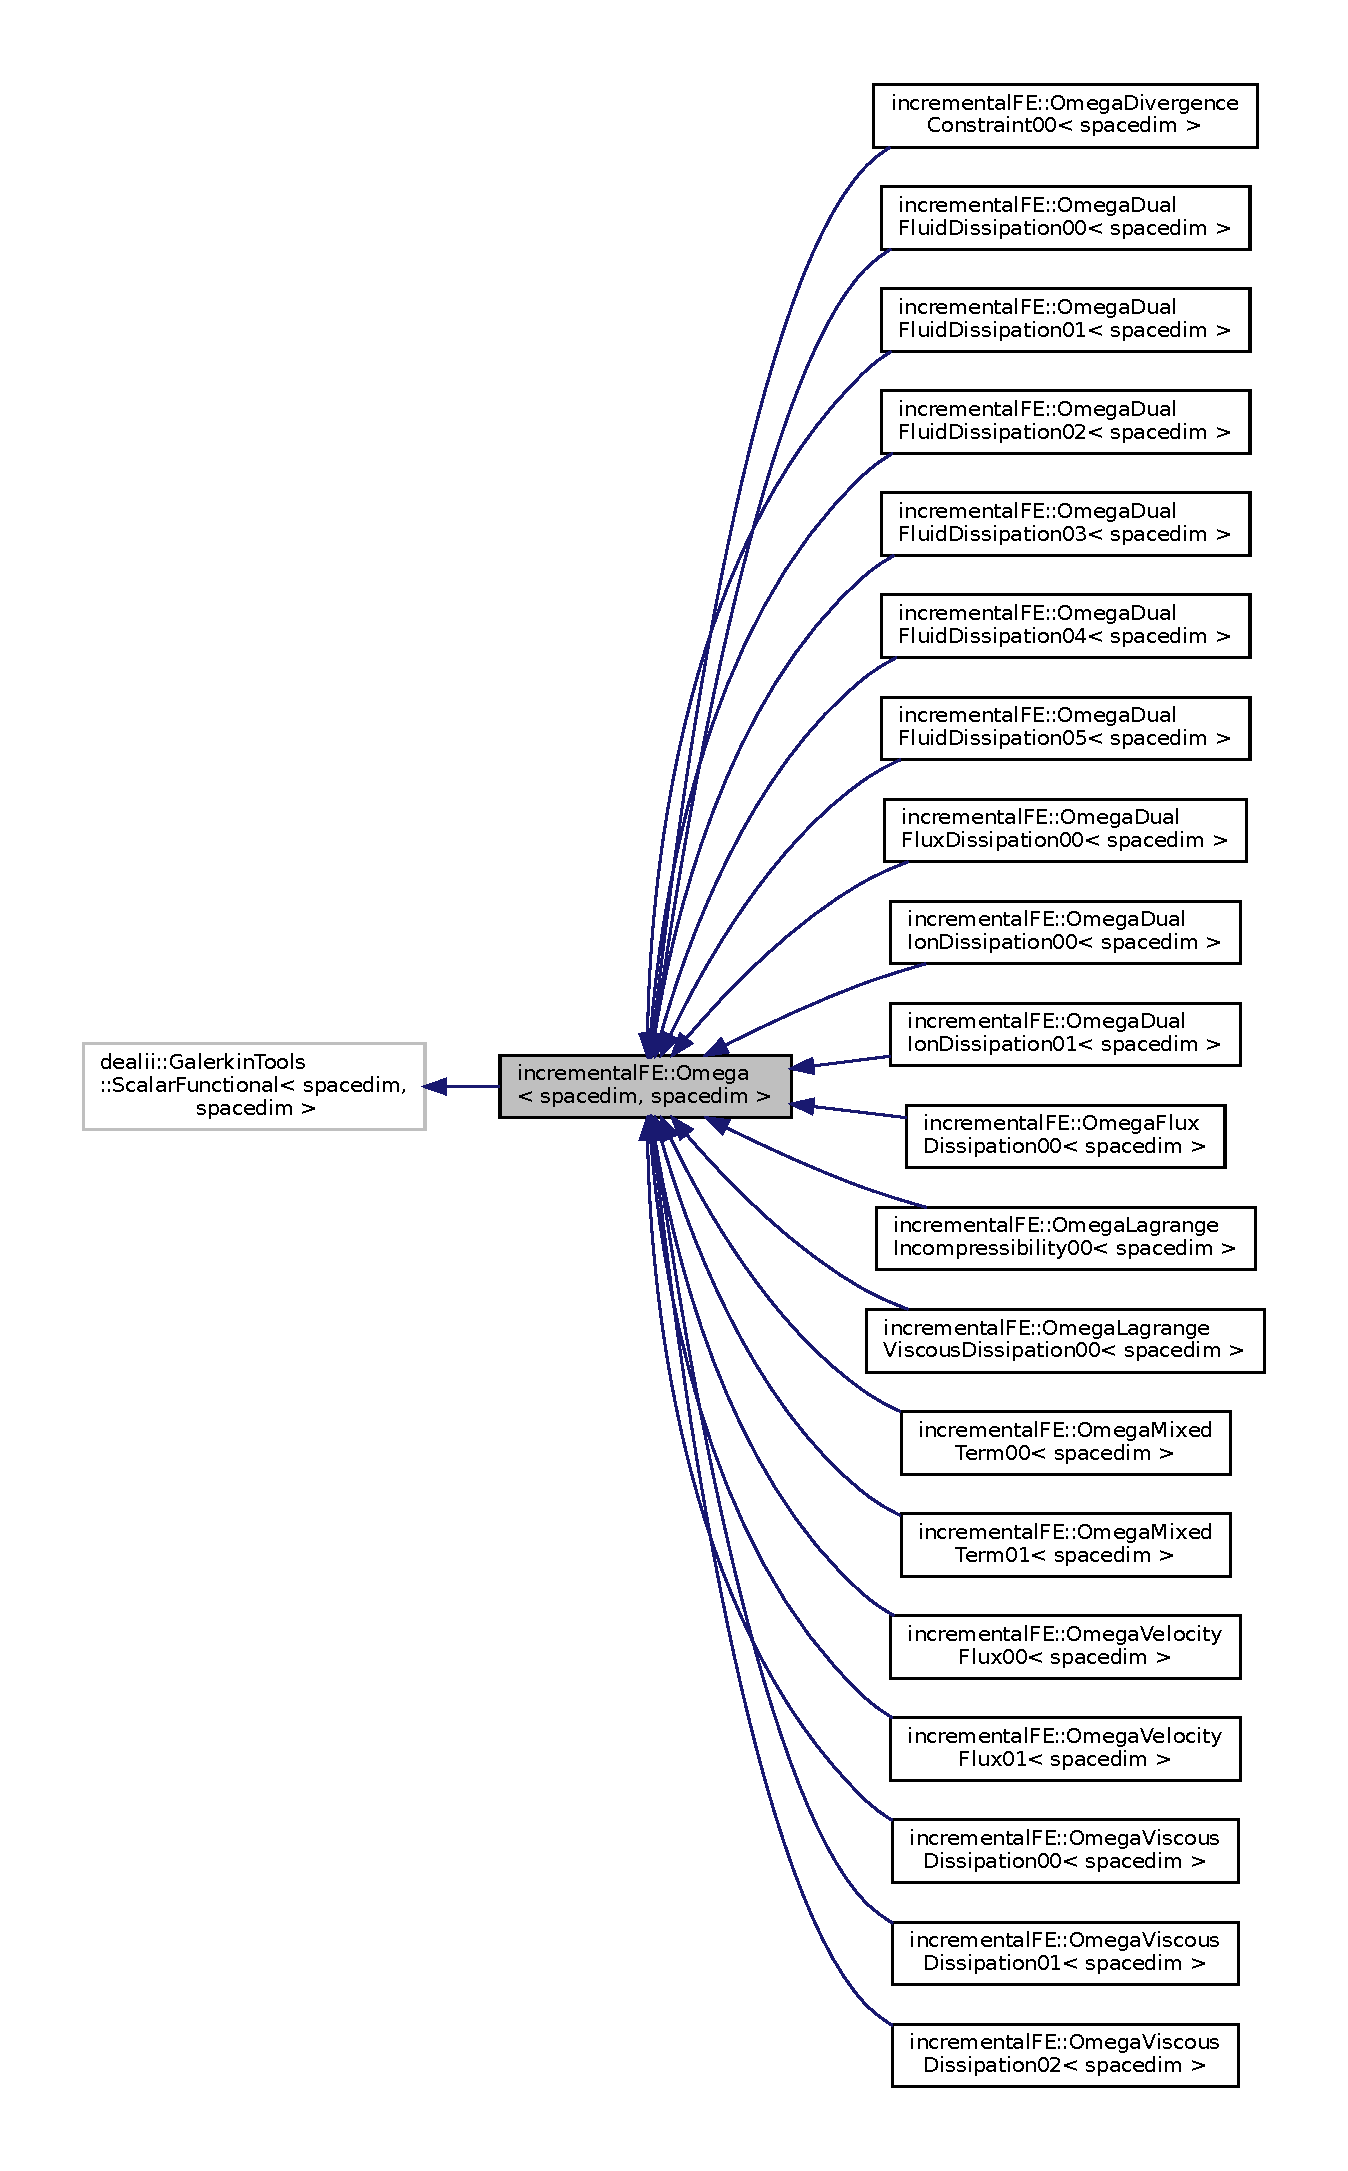
\includegraphics[width=350pt]{classincremental_f_e_1_1_omega_3_01spacedim_00_01spacedim_01_4__inherit__graph}
\end{center}
\end{figure}


Collaboration diagram for incremental\+FE\+:\+:Omega$<$ spacedim, spacedim $>$\+:\nopagebreak
\begin{figure}[H]
\begin{center}
\leavevmode
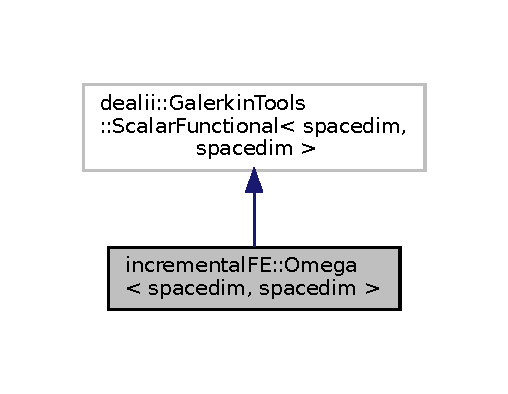
\includegraphics[width=229pt]{classincremental_f_e_1_1_omega_3_01spacedim_00_01spacedim_01_4__coll__graph}
\end{center}
\end{figure}
\subsection*{Public Member Functions}
\begin{DoxyCompactItemize}
\item 
\hyperlink{classincremental_f_e_1_1_omega_3_01spacedim_00_01spacedim_01_4_aa83ba9eb9e17b3b7ed6c573c172c4375}{Omega} (const std\+::vector$<$ dealii\+::\+Galerkin\+Tools\+::\+Dependent\+Field$<$ spacedim, spacedim $>$$>$ e\+\_\+omega, const std\+::set$<$ {\bf dealii\+::types\+::material\+\_\+id} $>$ domain\+\_\+of\+\_\+integration, const dealii\+::\+Quadrature$<$ spacedim $>$ quadrature, \hyperlink{classincremental_f_e_1_1_global_data_incremental_f_e}{Global\+Data\+Incremental\+FE}$<$ spacedim $>$ \&\hyperlink{classincremental_f_e_1_1_omega_3_01spacedim_00_01spacedim_01_4_afffe781a5a2032ec003032adc78e1bf3}{global\+\_\+data}, const unsigned int n\+\_\+v\+\_\+dot, const unsigned int n\+\_\+q\+\_\+dot, const unsigned int \hyperlink{classincremental_f_e_1_1_omega_3_01spacedim_00_01spacedim_01_4_a7f1db416dd6b487504856959c7253b53}{n\+\_\+mu}, const unsigned int \hyperlink{classincremental_f_e_1_1_omega_3_01spacedim_00_01spacedim_01_4_a708fdb9951f4879eaa020219f19db115}{n\+\_\+q}, const unsigned int \hyperlink{classincremental_f_e_1_1_omega_3_01spacedim_00_01spacedim_01_4_a6c95d57122261e8a2e26d3818251bc9b}{method}, const double \hyperlink{classincremental_f_e_1_1_omega_3_01spacedim_00_01spacedim_01_4_ad881c36804cc027c301f4f069756c2db}{alpha}=0.\+0, const std\+::string name=\char`\"{}Omega\char`\"{})
\item 
virtual \hyperlink{classincremental_f_e_1_1_omega_3_01spacedim_00_01spacedim_01_4_a9299cef8c66dd19302381f1c7b4d5c4c}{$\sim$\+Omega} ()=default
\item 
virtual bool \hyperlink{classincremental_f_e_1_1_omega_3_01spacedim_00_01spacedim_01_4_a40131354ef0a28ca48a0e6c9ed33aa33}{get\+\_\+values\+\_\+and\+\_\+derivatives} (const {\bf dealii\+::\+Vector}$<$ double $>$ \&{\bf values}, const double t, const dealii\+::\+Point$<$ spacedim $>$ \&x, double \&omega, {\bf dealii\+::\+Vector}$<$ double $>$ \&d\+\_\+omega, dealii\+::\+Full\+Matrix$<$ double $>$ \&d2\+\_\+omega, const std\+::tuple$<$ bool, bool, bool $>$ requested\+\_\+quantities, const bool compute\+\_\+d2q) const =0
\item 
bool \hyperlink{classincremental_f_e_1_1_omega_3_01spacedim_00_01spacedim_01_4_a183af2dde75d7b92afa02fdbf0216d85}{get\+\_\+h\+\_\+omega} (const {\bf dealii\+::\+Vector}$<$ double $>$ \&e\+\_\+omega, const std\+::vector$<$ {\bf dealii\+::\+Vector}$<$ double $>$$>$ \&e\+\_\+omega\+\_\+ref\+\_\+sets, {\bf dealii\+::\+Vector}$<$ double $>$ \&hidden\+\_\+vars, const dealii\+::\+Point$<$ spacedim $>$ \&x, double \&h\+\_\+omega, {\bf dealii\+::\+Vector}$<$ double $>$ \&h\+\_\+omega\+\_\+1, dealii\+::\+Full\+Matrix$<$ double $>$ \&h\+\_\+omega\+\_\+2, const std\+::tuple$<$ bool, bool, bool $>$ requested\+\_\+quantities) const final
\end{DoxyCompactItemize}
\subsection*{Public Attributes}
\begin{DoxyCompactItemize}
\item 
const unsigned int \hyperlink{classincremental_f_e_1_1_omega_3_01spacedim_00_01spacedim_01_4_ae34ad644385b50d04d1b04e42c8a5b28}{n\+\_\+v\+\_\+q\+\_\+dot}
\item 
const unsigned int \hyperlink{classincremental_f_e_1_1_omega_3_01spacedim_00_01spacedim_01_4_a7f1db416dd6b487504856959c7253b53}{n\+\_\+mu}
\item 
const unsigned int \hyperlink{classincremental_f_e_1_1_omega_3_01spacedim_00_01spacedim_01_4_a708fdb9951f4879eaa020219f19db115}{n\+\_\+q}
\end{DoxyCompactItemize}
\subsection*{Private Attributes}
\begin{DoxyCompactItemize}
\item 
const dealii\+::\+Smart\+Pointer$<$ \hyperlink{classincremental_f_e_1_1_global_data_incremental_f_e}{Global\+Data\+Incremental\+FE}$<$ spacedim $>$ $>$ \hyperlink{classincremental_f_e_1_1_omega_3_01spacedim_00_01spacedim_01_4_afffe781a5a2032ec003032adc78e1bf3}{global\+\_\+data}
\item 
const double \hyperlink{classincremental_f_e_1_1_omega_3_01spacedim_00_01spacedim_01_4_ad881c36804cc027c301f4f069756c2db}{alpha}
\item 
const unsigned int \hyperlink{classincremental_f_e_1_1_omega_3_01spacedim_00_01spacedim_01_4_a6c95d57122261e8a2e26d3818251bc9b}{method}
\end{DoxyCompactItemize}


\subsection{Detailed Description}
\subsubsection*{template$<$unsigned int spacedim$>$\\*
class incremental\+F\+E\+::\+Omega$<$ spacedim, spacedim $>$}

Class defining the time discrete approximation of a domain related scalar functional with the integrand

$ h^\Omega_\rho = \omega(\dot{v}, \dot{q}, \mu, q; t) $,

where $\dot{v}$, $\dot{q}$, $\mu$, and $q$ may be vectors.

The time discrete approximation is done either by Miehe\textquotesingle{}s method, by the $\alpha$-\/family, or by the modified $\alpha$-\/family. 

\subsection{Constructor \& Destructor Documentation}
\index{incremental\+F\+E\+::\+Omega$<$ spacedim, spacedim $>$@{incremental\+F\+E\+::\+Omega$<$ spacedim, spacedim $>$}!Omega@{Omega}}
\index{Omega@{Omega}!incremental\+F\+E\+::\+Omega$<$ spacedim, spacedim $>$@{incremental\+F\+E\+::\+Omega$<$ spacedim, spacedim $>$}}
\subsubsection[{\texorpdfstring{Omega(const std\+::vector$<$ dealii\+::\+Galerkin\+Tools\+::\+Dependent\+Field$<$ spacedim, spacedim $>$$>$ e\+\_\+omega, const std\+::set$<$ dealii\+::types\+::material\+\_\+id $>$ domain\+\_\+of\+\_\+integration, const dealii\+::\+Quadrature$<$ spacedim $>$ quadrature, Global\+Data\+Incremental\+F\+E$<$ spacedim $>$ \&global\+\_\+data, const unsigned int n\+\_\+v\+\_\+dot, const unsigned int n\+\_\+q\+\_\+dot, const unsigned int n\+\_\+mu, const unsigned int n\+\_\+q, const unsigned int method, const double alpha=0.\+0, const std\+::string name=""Omega"")}{Omega(const std::vector< dealii::GalerkinTools::DependentField< spacedim, spacedim >> e_omega, const std::set< dealii::types::material_id > domain_of_integration, const dealii::Quadrature< spacedim > quadrature, GlobalDataIncrementalFE< spacedim > &global_data, const unsigned int n_v_dot, const unsigned int n_q_dot, const unsigned int n_mu, const unsigned int n_q, const unsigned int method, const double alpha=0.0, const std::string name="Omega")}}]{\setlength{\rightskip}{0pt plus 5cm}template$<$unsigned int spacedim$>$ {\bf incremental\+F\+E\+::\+Omega}$<$ spacedim, spacedim $>$\+::{\bf Omega} (
\begin{DoxyParamCaption}
\item[{const std\+::vector$<$ dealii\+::\+Galerkin\+Tools\+::\+Dependent\+Field$<$ spacedim, spacedim $>$$>$}]{e\+\_\+omega, }
\item[{const std\+::set$<$ {\bf dealii\+::types\+::material\+\_\+id} $>$}]{domain\+\_\+of\+\_\+integration, }
\item[{const dealii\+::\+Quadrature$<$ spacedim $>$}]{quadrature, }
\item[{{\bf Global\+Data\+Incremental\+FE}$<$ spacedim $>$ \&}]{global\+\_\+data, }
\item[{const unsigned int}]{n\+\_\+v\+\_\+dot, }
\item[{const unsigned int}]{n\+\_\+q\+\_\+dot, }
\item[{const unsigned int}]{n\+\_\+mu, }
\item[{const unsigned int}]{n\+\_\+q, }
\item[{const unsigned int}]{method, }
\item[{const double}]{alpha = {\ttfamily 0.0}, }
\item[{const std\+::string}]{name = {\ttfamily \char`\"{}Omega$<$~spacedim,~spacedim~$>$\char`\"{}}}
\end{DoxyParamCaption}
)}\hypertarget{classincremental_f_e_1_1_omega_3_01spacedim_00_01spacedim_01_4_aa83ba9eb9e17b3b7ed6c573c172c4375}{}\label{classincremental_f_e_1_1_omega_3_01spacedim_00_01spacedim_01_4_aa83ba9eb9e17b3b7ed6c573c172c4375}
Constructor


\begin{DoxyParams}[1]{Parameters}
\mbox{\tt in}  & {\em e\+\_\+omega} & Dependent fields (in the order $\dot{v}$, $\dot{q}$, $\mu$, $q$)\\
\hline
\mbox{\tt in}  & {\em domain\+\_\+of\+\_\+integration} & {\bf Scalar\+Functional\+::domain\+\_\+of\+\_\+integration}\\
\hline
\mbox{\tt in}  & {\em quadrature} & {\bf Scalar\+Functional\+::quadrature}\\
\hline
\mbox{\tt in}  & {\em global\+\_\+data} & \hyperlink{classincremental_f_e_1_1_omega_abd23d288a7a4a43f9b528be968cd2113}{Omega\+::global\+\_\+data}\\
\hline
\mbox{\tt in}  & {\em n\+\_\+v\+\_\+dot} & The number of $\dot{v}$\\
\hline
\mbox{\tt in}  & {\em n\+\_\+q\+\_\+dot} & The number of $\dot{q}$\\
\hline
\mbox{\tt in}  & {\em n\+\_\+mu} & The number of $\mu$\\
\hline
\mbox{\tt in}  & {\em n\+\_\+q} & The number of $q$\\
\hline
\mbox{\tt in}  & {\em method} & \hyperlink{classincremental_f_e_1_1_omega_a7600d263ebf98129629e44fa67e8a58c}{Omega\+::method}\\
\hline
\mbox{\tt in}  & {\em alpha} & \hyperlink{classincremental_f_e_1_1_omega_a891688560ec0ad8dc5a0058a7b400269}{Omega\+::alpha}\\
\hline
\mbox{\tt in}  & {\em name} & {\bf Scalar\+Functional\+::name} \\
\hline
\end{DoxyParams}
\index{incremental\+F\+E\+::\+Omega$<$ spacedim, spacedim $>$@{incremental\+F\+E\+::\+Omega$<$ spacedim, spacedim $>$}!````~Omega@{$\sim$\+Omega}}
\index{````~Omega@{$\sim$\+Omega}!incremental\+F\+E\+::\+Omega$<$ spacedim, spacedim $>$@{incremental\+F\+E\+::\+Omega$<$ spacedim, spacedim $>$}}
\subsubsection[{\texorpdfstring{$\sim$\+Omega()=default}{~Omega()=default}}]{\setlength{\rightskip}{0pt plus 5cm}template$<$unsigned int spacedim$>$ virtual {\bf incremental\+F\+E\+::\+Omega}$<$ spacedim, spacedim $>$\+::$\sim${\bf Omega} (
\begin{DoxyParamCaption}
{}
\end{DoxyParamCaption}
)\hspace{0.3cm}{\ttfamily [virtual]}, {\ttfamily [default]}}\hypertarget{classincremental_f_e_1_1_omega_3_01spacedim_00_01spacedim_01_4_a9299cef8c66dd19302381f1c7b4d5c4c}{}\label{classincremental_f_e_1_1_omega_3_01spacedim_00_01spacedim_01_4_a9299cef8c66dd19302381f1c7b4d5c4c}
Destructor 

\subsection{Member Function Documentation}
\index{incremental\+F\+E\+::\+Omega$<$ spacedim, spacedim $>$@{incremental\+F\+E\+::\+Omega$<$ spacedim, spacedim $>$}!get\+\_\+h\+\_\+omega@{get\+\_\+h\+\_\+omega}}
\index{get\+\_\+h\+\_\+omega@{get\+\_\+h\+\_\+omega}!incremental\+F\+E\+::\+Omega$<$ spacedim, spacedim $>$@{incremental\+F\+E\+::\+Omega$<$ spacedim, spacedim $>$}}
\subsubsection[{\texorpdfstring{get\+\_\+h\+\_\+omega(const dealii\+::\+Vector$<$ double $>$ \&e\+\_\+omega, const std\+::vector$<$ dealii\+::\+Vector$<$ double $>$$>$ \&e\+\_\+omega\+\_\+ref\+\_\+sets, dealii\+::\+Vector$<$ double $>$ \&hidden\+\_\+vars, const dealii\+::\+Point$<$ spacedim $>$ \&x, double \&h\+\_\+omega, dealii\+::\+Vector$<$ double $>$ \&h\+\_\+omega\+\_\+1, dealii\+::\+Full\+Matrix$<$ double $>$ \&h\+\_\+omega\+\_\+2, const std\+::tuple$<$ bool, bool, bool $>$ requested\+\_\+quantities) const final}{get_h_omega(const dealii::Vector< double > &e_omega, const std::vector< dealii::Vector< double >> &e_omega_ref_sets, dealii::Vector< double > &hidden_vars, const dealii::Point< spacedim > &x, double &h_omega, dealii::Vector< double > &h_omega_1, dealii::FullMatrix< double > &h_omega_2, const std::tuple< bool, bool, bool > requested_quantities) const final}}]{\setlength{\rightskip}{0pt plus 5cm}template$<$unsigned int spacedim$>$ bool {\bf incremental\+F\+E\+::\+Omega}$<$ spacedim, spacedim $>$\+::get\+\_\+h\+\_\+omega (
\begin{DoxyParamCaption}
\item[{const {\bf dealii\+::\+Vector}$<$ double $>$ \&}]{e\+\_\+omega, }
\item[{const std\+::vector$<$ {\bf dealii\+::\+Vector}$<$ double $>$$>$ \&}]{e\+\_\+omega\+\_\+ref\+\_\+sets, }
\item[{{\bf dealii\+::\+Vector}$<$ double $>$ \&}]{hidden\+\_\+vars, }
\item[{const dealii\+::\+Point$<$ spacedim $>$ \&}]{x, }
\item[{double \&}]{h\+\_\+omega, }
\item[{{\bf dealii\+::\+Vector}$<$ double $>$ \&}]{h\+\_\+omega\+\_\+1, }
\item[{dealii\+::\+Full\+Matrix$<$ double $>$ \&}]{h\+\_\+omega\+\_\+2, }
\item[{const std\+::tuple$<$ bool, bool, bool $>$}]{requested\+\_\+quantities}
\end{DoxyParamCaption}
) const\hspace{0.3cm}{\ttfamily [final]}}\hypertarget{classincremental_f_e_1_1_omega_3_01spacedim_00_01spacedim_01_4_a183af2dde75d7b92afa02fdbf0216d85}{}\label{classincremental_f_e_1_1_omega_3_01spacedim_00_01spacedim_01_4_a183af2dde75d7b92afa02fdbf0216d85}
see {\bf Scalar\+Functional$<$spacedim, spacedim$>$\+::get\+\_\+h\+\_\+omega} \index{incremental\+F\+E\+::\+Omega$<$ spacedim, spacedim $>$@{incremental\+F\+E\+::\+Omega$<$ spacedim, spacedim $>$}!get\+\_\+values\+\_\+and\+\_\+derivatives@{get\+\_\+values\+\_\+and\+\_\+derivatives}}
\index{get\+\_\+values\+\_\+and\+\_\+derivatives@{get\+\_\+values\+\_\+and\+\_\+derivatives}!incremental\+F\+E\+::\+Omega$<$ spacedim, spacedim $>$@{incremental\+F\+E\+::\+Omega$<$ spacedim, spacedim $>$}}
\subsubsection[{\texorpdfstring{get\+\_\+values\+\_\+and\+\_\+derivatives(const dealii\+::\+Vector$<$ double $>$ \&values, const double t, const dealii\+::\+Point$<$ spacedim $>$ \&x, double \&omega, dealii\+::\+Vector$<$ double $>$ \&d\+\_\+omega, dealii\+::\+Full\+Matrix$<$ double $>$ \&d2\+\_\+omega, const std\+::tuple$<$ bool, bool, bool $>$ requested\+\_\+quantities, const bool compute\+\_\+d2q) const =0}{get_values_and_derivatives(const dealii::Vector< double > &values, const double t, const dealii::Point< spacedim > &x, double &omega, dealii::Vector< double > &d_omega, dealii::FullMatrix< double > &d2_omega, const std::tuple< bool, bool, bool > requested_quantities, const bool compute_d2q) const =0}}]{\setlength{\rightskip}{0pt plus 5cm}template$<$unsigned int spacedim$>$ virtual bool {\bf incremental\+F\+E\+::\+Omega}$<$ spacedim, spacedim $>$\+::get\+\_\+values\+\_\+and\+\_\+derivatives (
\begin{DoxyParamCaption}
\item[{const {\bf dealii\+::\+Vector}$<$ double $>$ \&}]{values, }
\item[{const double}]{t, }
\item[{const dealii\+::\+Point$<$ spacedim $>$ \&}]{x, }
\item[{double \&}]{omega, }
\item[{{\bf dealii\+::\+Vector}$<$ double $>$ \&}]{d\+\_\+omega, }
\item[{dealii\+::\+Full\+Matrix$<$ double $>$ \&}]{d2\+\_\+omega, }
\item[{const std\+::tuple$<$ bool, bool, bool $>$}]{requested\+\_\+quantities, }
\item[{const bool}]{compute\+\_\+d2q}
\end{DoxyParamCaption}
) const\hspace{0.3cm}{\ttfamily [pure virtual]}}\hypertarget{classincremental_f_e_1_1_omega_3_01spacedim_00_01spacedim_01_4_a40131354ef0a28ca48a0e6c9ed33aa33}{}\label{classincremental_f_e_1_1_omega_3_01spacedim_00_01spacedim_01_4_a40131354ef0a28ca48a0e6c9ed33aa33}
This function defines $\omega$ and needs to be implemented by classes inheriting from this class


\begin{DoxyParams}[1]{Parameters}
\mbox{\tt in}  & {\em values} & Values at which $\omega$ and its derivatives are evaluated (in the order $\dot{v}$, $\dot{q}$, $\mu$, $q$)\\
\hline
\mbox{\tt in}  & {\em t} & Time at which $\omega$ is evaluated\\
\hline
\mbox{\tt in}  & {\em x} & Position\\
\hline
\mbox{\tt out}  & {\em omega} & Value of $\omega$\\
\hline
\mbox{\tt out}  & {\em d\+\_\+omega} & Values of first derivatives of $\omega$ w.\+r.\+t. $\dot{v}$, $\dot{q}$, $\mu$ (in this order)\\
\hline
\mbox{\tt out}  & {\em d2\+\_\+omega} & Values of second derivatives of $\omega$ w.\+r.\+t. $\dot{v}$, $\dot{q}$, $\mu$ (in this order). If {\ttfamily compute\+\_\+d2q} == {\ttfamily true}, also the derivatives of {\ttfamily d\+\_\+omega} w.\+r.\+t. $q$ need to be computed. In this case, {\ttfamily d2\+\_\+omega} is initialized to the size \hyperlink{classincremental_f_e_1_1_omega_a7fa938b26804b0dc15726f3423332880}{Omega\+::n\+\_\+v\+\_\+q\+\_\+dot} + \hyperlink{classincremental_f_e_1_1_omega_a322340b50451ab46f91cdcec95248f16}{Omega\+::n\+\_\+mu} x \hyperlink{classincremental_f_e_1_1_omega_a7fa938b26804b0dc15726f3423332880}{Omega\+::n\+\_\+v\+\_\+q\+\_\+dot} + \hyperlink{classincremental_f_e_1_1_omega_a322340b50451ab46f91cdcec95248f16}{Omega\+::n\+\_\+mu} + \hyperlink{classincremental_f_e_1_1_omega_addbf75c949792f6340ea40164a2bfee3}{Omega\+::n\+\_\+q}, so that derivatives of {\ttfamily d\+\_\+omega} w.\+r.\+t. $q$ can be stored in the rightmost part of the matrix.\\
\hline
\mbox{\tt in}  & {\em requested\+\_\+quantities} & Tuple indicating which of the quantities {\ttfamily omega}, {\ttfamily d\+\_\+omega}, {\ttfamily d2\+\_\+omega} are to be computed. Note that only those quantities are passed in initialized to the correct size, which are actually requested\\
\hline
\mbox{\tt in}  & {\em compute\+\_\+d2q} & If {\ttfamily true}, also compute second derivatives w.\+r.\+t. $q$\\
\hline
\end{DoxyParams}
\begin{DoxyReturn}{Returns}
{\ttfamily true} indicates that an error has occurred in the function 
\end{DoxyReturn}


Implemented in \hyperlink{classincremental_f_e_1_1_omega_dual_fluid_dissipation01_a3c58b42747ba2c2bed05fa670cf55fb5}{incremental\+F\+E\+::\+Omega\+Dual\+Fluid\+Dissipation01$<$ spacedim $>$}, \hyperlink{classincremental_f_e_1_1_omega_dual_fluid_dissipation00_a505f97cabdd9375fe76b714c28088ca6}{incremental\+F\+E\+::\+Omega\+Dual\+Fluid\+Dissipation00$<$ spacedim $>$}, \hyperlink{classincremental_f_e_1_1_omega_dual_ion_dissipation00_a0222bc5e8dfcc93728c230c604439332}{incremental\+F\+E\+::\+Omega\+Dual\+Ion\+Dissipation00$<$ spacedim $>$}, \hyperlink{classincremental_f_e_1_1_omega_divergence_constraint00_a56323a14c158f9008621a9a5d77f1be8}{incremental\+F\+E\+::\+Omega\+Divergence\+Constraint00$<$ spacedim $>$}, \hyperlink{classincremental_f_e_1_1_omega_mixed_term01_a6fe47df6c774ba07cb3455616997dfe7}{incremental\+F\+E\+::\+Omega\+Mixed\+Term01$<$ spacedim $>$}, \hyperlink{classincremental_f_e_1_1_omega_mixed_term00_abf975855eb0155318ad152e7fbac11d1}{incremental\+F\+E\+::\+Omega\+Mixed\+Term00$<$ spacedim $>$}, \hyperlink{classincremental_f_e_1_1_omega_dual_flux_dissipation00_a27833d3c88054ddf2231a32c6c6b2d2d}{incremental\+F\+E\+::\+Omega\+Dual\+Flux\+Dissipation00$<$ spacedim $>$}, and \hyperlink{classincremental_f_e_1_1_omega_flux_dissipation00_a7b9ccca9346b229a5e7f4f2254d932ec}{incremental\+F\+E\+::\+Omega\+Flux\+Dissipation00$<$ spacedim $>$}.



\subsection{Member Data Documentation}
\index{incremental\+F\+E\+::\+Omega$<$ spacedim, spacedim $>$@{incremental\+F\+E\+::\+Omega$<$ spacedim, spacedim $>$}!alpha@{alpha}}
\index{alpha@{alpha}!incremental\+F\+E\+::\+Omega$<$ spacedim, spacedim $>$@{incremental\+F\+E\+::\+Omega$<$ spacedim, spacedim $>$}}
\subsubsection[{\texorpdfstring{alpha}{alpha}}]{\setlength{\rightskip}{0pt plus 5cm}template$<$unsigned int spacedim$>$ const double {\bf incremental\+F\+E\+::\+Omega}$<$ spacedim, spacedim $>$\+::alpha\hspace{0.3cm}{\ttfamily [private]}}\hypertarget{classincremental_f_e_1_1_omega_3_01spacedim_00_01spacedim_01_4_ad881c36804cc027c301f4f069756c2db}{}\label{classincremental_f_e_1_1_omega_3_01spacedim_00_01spacedim_01_4_ad881c36804cc027c301f4f069756c2db}
Numerical parameter between {\ttfamily 0} and {\ttfamily 1}.

This parameter is only used for the $\alpha$-\/family and the modified $\alpha$-\/family \index{incremental\+F\+E\+::\+Omega$<$ spacedim, spacedim $>$@{incremental\+F\+E\+::\+Omega$<$ spacedim, spacedim $>$}!global\+\_\+data@{global\+\_\+data}}
\index{global\+\_\+data@{global\+\_\+data}!incremental\+F\+E\+::\+Omega$<$ spacedim, spacedim $>$@{incremental\+F\+E\+::\+Omega$<$ spacedim, spacedim $>$}}
\subsubsection[{\texorpdfstring{global\+\_\+data}{global_data}}]{\setlength{\rightskip}{0pt plus 5cm}template$<$unsigned int spacedim$>$ const dealii\+::\+Smart\+Pointer$<${\bf Global\+Data\+Incremental\+FE}$<$spacedim$>$ $>$ {\bf incremental\+F\+E\+::\+Omega}$<$ spacedim, spacedim $>$\+::global\+\_\+data\hspace{0.3cm}{\ttfamily [private]}}\hypertarget{classincremental_f_e_1_1_omega_3_01spacedim_00_01spacedim_01_4_afffe781a5a2032ec003032adc78e1bf3}{}\label{classincremental_f_e_1_1_omega_3_01spacedim_00_01spacedim_01_4_afffe781a5a2032ec003032adc78e1bf3}
global data object \index{incremental\+F\+E\+::\+Omega$<$ spacedim, spacedim $>$@{incremental\+F\+E\+::\+Omega$<$ spacedim, spacedim $>$}!method@{method}}
\index{method@{method}!incremental\+F\+E\+::\+Omega$<$ spacedim, spacedim $>$@{incremental\+F\+E\+::\+Omega$<$ spacedim, spacedim $>$}}
\subsubsection[{\texorpdfstring{method}{method}}]{\setlength{\rightskip}{0pt plus 5cm}template$<$unsigned int spacedim$>$ const unsigned int {\bf incremental\+F\+E\+::\+Omega}$<$ spacedim, spacedim $>$\+::method\hspace{0.3cm}{\ttfamily [private]}}\hypertarget{classincremental_f_e_1_1_omega_3_01spacedim_00_01spacedim_01_4_a6c95d57122261e8a2e26d3818251bc9b}{}\label{classincremental_f_e_1_1_omega_3_01spacedim_00_01spacedim_01_4_a6c95d57122261e8a2e26d3818251bc9b}
Temporal discretization ({\ttfamily 0}\+: Miehe\textquotesingle{}s method, {\ttfamily 1}\+: $\alpha$-\/family, {\ttfamily 2}\+: modified $\alpha$-\/family) \index{incremental\+F\+E\+::\+Omega$<$ spacedim, spacedim $>$@{incremental\+F\+E\+::\+Omega$<$ spacedim, spacedim $>$}!n\+\_\+mu@{n\+\_\+mu}}
\index{n\+\_\+mu@{n\+\_\+mu}!incremental\+F\+E\+::\+Omega$<$ spacedim, spacedim $>$@{incremental\+F\+E\+::\+Omega$<$ spacedim, spacedim $>$}}
\subsubsection[{\texorpdfstring{n\+\_\+mu}{n_mu}}]{\setlength{\rightskip}{0pt plus 5cm}template$<$unsigned int spacedim$>$ const unsigned int {\bf incremental\+F\+E\+::\+Omega}$<$ spacedim, spacedim $>$\+::n\+\_\+mu}\hypertarget{classincremental_f_e_1_1_omega_3_01spacedim_00_01spacedim_01_4_a7f1db416dd6b487504856959c7253b53}{}\label{classincremental_f_e_1_1_omega_3_01spacedim_00_01spacedim_01_4_a7f1db416dd6b487504856959c7253b53}
Number of Lagrangian multiplier variables \index{incremental\+F\+E\+::\+Omega$<$ spacedim, spacedim $>$@{incremental\+F\+E\+::\+Omega$<$ spacedim, spacedim $>$}!n\+\_\+q@{n\+\_\+q}}
\index{n\+\_\+q@{n\+\_\+q}!incremental\+F\+E\+::\+Omega$<$ spacedim, spacedim $>$@{incremental\+F\+E\+::\+Omega$<$ spacedim, spacedim $>$}}
\subsubsection[{\texorpdfstring{n\+\_\+q}{n_q}}]{\setlength{\rightskip}{0pt plus 5cm}template$<$unsigned int spacedim$>$ const unsigned int {\bf incremental\+F\+E\+::\+Omega}$<$ spacedim, spacedim $>$\+::n\+\_\+q}\hypertarget{classincremental_f_e_1_1_omega_3_01spacedim_00_01spacedim_01_4_a708fdb9951f4879eaa020219f19db115}{}\label{classincremental_f_e_1_1_omega_3_01spacedim_00_01spacedim_01_4_a708fdb9951f4879eaa020219f19db115}
Number of state variables \index{incremental\+F\+E\+::\+Omega$<$ spacedim, spacedim $>$@{incremental\+F\+E\+::\+Omega$<$ spacedim, spacedim $>$}!n\+\_\+v\+\_\+q\+\_\+dot@{n\+\_\+v\+\_\+q\+\_\+dot}}
\index{n\+\_\+v\+\_\+q\+\_\+dot@{n\+\_\+v\+\_\+q\+\_\+dot}!incremental\+F\+E\+::\+Omega$<$ spacedim, spacedim $>$@{incremental\+F\+E\+::\+Omega$<$ spacedim, spacedim $>$}}
\subsubsection[{\texorpdfstring{n\+\_\+v\+\_\+q\+\_\+dot}{n_v_q_dot}}]{\setlength{\rightskip}{0pt plus 5cm}template$<$unsigned int spacedim$>$ const unsigned int {\bf incremental\+F\+E\+::\+Omega}$<$ spacedim, spacedim $>$\+::n\+\_\+v\+\_\+q\+\_\+dot}\hypertarget{classincremental_f_e_1_1_omega_3_01spacedim_00_01spacedim_01_4_ae34ad644385b50d04d1b04e42c8a5b28}{}\label{classincremental_f_e_1_1_omega_3_01spacedim_00_01spacedim_01_4_ae34ad644385b50d04d1b04e42c8a5b28}
Sum of components in $\dot{v}$ and $\dot{q}$ 

The documentation for this class was generated from the following file\+:\begin{DoxyCompactItemize}
\item 
/home/sst/code/\+Incremental\+F\+E/\+Incremental\+F\+E/include/incremental\+\_\+fe/scalar\+\_\+functionals/\hyperlink{omega_8h}{omega.\+h}\end{DoxyCompactItemize}

\hypertarget{classincremental_f_e_1_1_omega_displacement_coupling00}{}\doxysection{incremental\+FE\+::Omega\+Displacement\+Coupling00$<$ spacedim $>$ Class Template Reference}
\label{classincremental_f_e_1_1_omega_displacement_coupling00}\index{incrementalFE::OmegaDisplacementCoupling00$<$ spacedim $>$@{incrementalFE::OmegaDisplacementCoupling00$<$ spacedim $>$}}


{\ttfamily \#include $<$omega\+\_\+lib.\+h$>$}



Inheritance diagram for incremental\+FE\+::Omega\+Displacement\+Coupling00$<$ spacedim $>$\+:\nopagebreak
\begin{figure}[H]
\begin{center}
\leavevmode
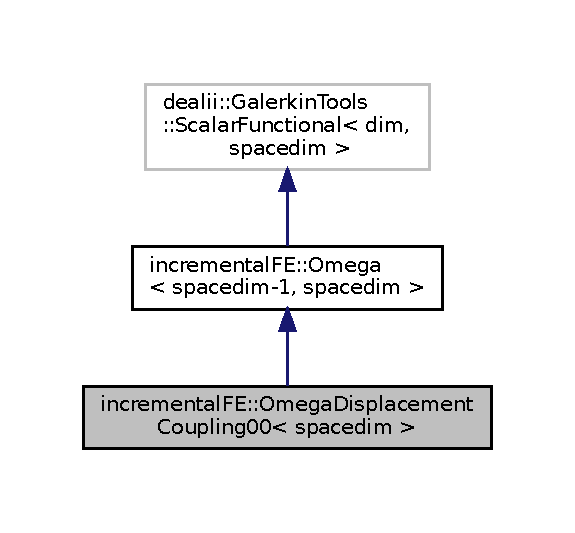
\includegraphics[width=276pt]{classincremental_f_e_1_1_omega_displacement_coupling00__inherit__graph}
\end{center}
\end{figure}


Collaboration diagram for incremental\+FE\+::Omega\+Displacement\+Coupling00$<$ spacedim $>$\+:\nopagebreak
\begin{figure}[H]
\begin{center}
\leavevmode
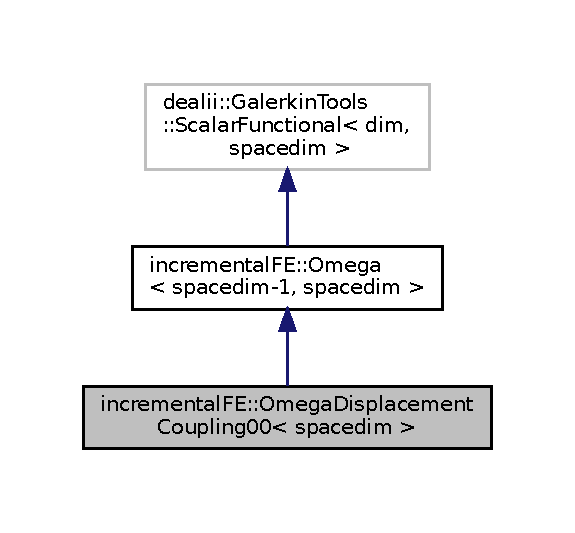
\includegraphics[width=276pt]{classincremental_f_e_1_1_omega_displacement_coupling00__coll__graph}
\end{center}
\end{figure}
\doxysubsection*{Public Member Functions}
\begin{DoxyCompactItemize}
\item 
\mbox{\hyperlink{classincremental_f_e_1_1_omega_displacement_coupling00_a2ab6b3cc56b180909d7eba7942757f1e}{Omega\+Displacement\+Coupling00}} (const std\+::vector$<$ dealii\+::\+Galerkin\+Tools\+::\+Dependent\+Field$<$ spacedim-\/1, spacedim $>$$>$ e\+\_\+sigma, const std\+::set$<$ \textbf{ dealii\+::types\+::material\+\_\+id} $>$ domain\+\_\+of\+\_\+integration, const dealii\+::\+Quadrature$<$ spacedim-\/1 $>$ quadrature, \mbox{\hyperlink{classincremental_f_e_1_1_global_data_incremental_f_e}{Global\+Data\+Incremental\+FE}}$<$ spacedim $>$ \&\mbox{\hyperlink{classincremental_f_e_1_1_omega_abd23d288a7a4a43f9b528be968cd2113}{global\+\_\+data}}, const bool \mbox{\hyperlink{classincremental_f_e_1_1_omega_displacement_coupling00_a1dc29cbc64a8477b06f1a01472783e5e}{u\+\_\+1\+\_\+as\+\_\+parameter}}, const unsigned int \mbox{\hyperlink{classincremental_f_e_1_1_omega_a7600d263ebf98129629e44fa67e8a58c}{method}}, const double \mbox{\hyperlink{classincremental_f_e_1_1_omega_a891688560ec0ad8dc5a0058a7b400269}{alpha}}=0.\+0)
\item 
bool \mbox{\hyperlink{classincremental_f_e_1_1_omega_displacement_coupling00_af4d521887a8dad96e5f76f21fd7a5f1e}{get\+\_\+values\+\_\+and\+\_\+derivatives}} (const \textbf{ dealii\+::\+Vector}$<$ double $>$ \&\textbf{ values}, const double, const dealii\+::\+Point$<$ spacedim $>$ \&, const dealii\+::\+Tensor$<$ 1, spacedim $>$ \&, double \&sigma, \textbf{ dealii\+::\+Vector}$<$ double $>$ \&d\+\_\+sigma, dealii\+::\+Full\+Matrix$<$ double $>$ \&d2\+\_\+sigma, const std\+::tuple$<$ bool, bool, bool $>$ requested\+\_\+quantities, const bool) const
\end{DoxyCompactItemize}
\doxysubsection*{Private Attributes}
\begin{DoxyCompactItemize}
\item 
const bool \mbox{\hyperlink{classincremental_f_e_1_1_omega_displacement_coupling00_a1dc29cbc64a8477b06f1a01472783e5e}{u\+\_\+1\+\_\+as\+\_\+parameter}}
\end{DoxyCompactItemize}
\doxysubsection*{Additional Inherited Members}


\doxysubsection{Detailed Description}
\subsubsection*{template$<$unsigned int spacedim$>$\newline
class incremental\+F\+E\+::\+Omega\+Displacement\+Coupling00$<$ spacedim $>$}

Class defining an interface related scalar functional with the integrand

$ h^\Sigma_\tau = \boldsymbol{t} \cdot \left( \boldsymbol{u}^0 - \boldsymbol{u}^1 \right) $

where $\boldsymbol{t}$ is a Lagrangian multiplier, $\boldsymbol{u}^0$ the displacement on the 0 side of the interface, and $\boldsymbol{u}^1$ the displacement on the 1 side of the interface.

Ordering of quantities in \textbf{ Scalar\+Functional\+::e\+\_\+sigma} \+:~\newline
\mbox{[}0\mbox{]} $u^0_x$~\newline
 \mbox{[}1\mbox{]} $u^0_y$~\newline
 \mbox{[}2\mbox{]} $u^0_z$~\newline
 \mbox{[}3\mbox{]} $u^1_x$~\newline
 \mbox{[}4\mbox{]} $u^1_y$~\newline
 \mbox{[}5\mbox{]} $u^1_z$~\newline
 \mbox{[}6\mbox{]} $t_x$~\newline
 \mbox{[}7\mbox{]} $t_y$~\newline
 \mbox{[}8\mbox{]} $t_z$~\newline
 

\doxysubsection{Constructor \& Destructor Documentation}
\mbox{\Hypertarget{classincremental_f_e_1_1_omega_displacement_coupling00_a2ab6b3cc56b180909d7eba7942757f1e}\label{classincremental_f_e_1_1_omega_displacement_coupling00_a2ab6b3cc56b180909d7eba7942757f1e}} 
\index{incrementalFE::OmegaDisplacementCoupling00$<$ spacedim $>$@{incrementalFE::OmegaDisplacementCoupling00$<$ spacedim $>$}!OmegaDisplacementCoupling00@{OmegaDisplacementCoupling00}}
\index{OmegaDisplacementCoupling00@{OmegaDisplacementCoupling00}!incrementalFE::OmegaDisplacementCoupling00$<$ spacedim $>$@{incrementalFE::OmegaDisplacementCoupling00$<$ spacedim $>$}}
\doxysubsubsection{\texorpdfstring{OmegaDisplacementCoupling00()}{OmegaDisplacementCoupling00()}}
{\footnotesize\ttfamily template$<$unsigned int spacedim$>$ \\
\mbox{\hyperlink{classincremental_f_e_1_1_omega_displacement_coupling00}{incremental\+F\+E\+::\+Omega\+Displacement\+Coupling00}}$<$ spacedim $>$\+::\mbox{\hyperlink{classincremental_f_e_1_1_omega_displacement_coupling00}{Omega\+Displacement\+Coupling00}} (\begin{DoxyParamCaption}\item[{const std\+::vector$<$ dealii\+::\+Galerkin\+Tools\+::\+Dependent\+Field$<$ spacedim-\/1, spacedim $>$$>$}]{e\+\_\+sigma,  }\item[{const std\+::set$<$ \textbf{ dealii\+::types\+::material\+\_\+id} $>$}]{domain\+\_\+of\+\_\+integration,  }\item[{const dealii\+::\+Quadrature$<$ spacedim-\/1 $>$}]{quadrature,  }\item[{\mbox{\hyperlink{classincremental_f_e_1_1_global_data_incremental_f_e}{Global\+Data\+Incremental\+FE}}$<$ spacedim $>$ \&}]{global\+\_\+data,  }\item[{const bool}]{u\+\_\+1\+\_\+as\+\_\+parameter,  }\item[{const unsigned int}]{method,  }\item[{const double}]{alpha = {\ttfamily 0.0} }\end{DoxyParamCaption})\hspace{0.3cm}{\ttfamily [inline]}}

Constructor


\begin{DoxyParams}[1]{Parameters}
\mbox{\texttt{ in}}  & {\em e\+\_\+sigma} & \textbf{ Scalar\+Functional\+::e\+\_\+sigma}\\
\hline
\mbox{\texttt{ in}}  & {\em domain\+\_\+of\+\_\+integration} & \textbf{ Scalar\+Functional\+::domain\+\_\+of\+\_\+integration}\\
\hline
\mbox{\texttt{ in}}  & {\em quadrature} & \textbf{ Scalar\+Functional\+::quadrature}\\
\hline
\mbox{\texttt{ in}}  & {\em global\+\_\+data} & \mbox{\hyperlink{classincremental_f_e_1_1_omega_abd23d288a7a4a43f9b528be968cd2113}{Omega\+::global\+\_\+data}}\\
\hline
\mbox{\texttt{ in}}  & {\em u\+\_\+1\+\_\+as\+\_\+parameter} & \mbox{\hyperlink{classincremental_f_e_1_1_omega_displacement_coupling00_a1dc29cbc64a8477b06f1a01472783e5e}{Omega\+Displacement\+Coupling00\+::u\+\_\+1\+\_\+as\+\_\+parameter}}\\
\hline
\mbox{\texttt{ in}}  & {\em method} & \mbox{\hyperlink{classincremental_f_e_1_1_omega_a7600d263ebf98129629e44fa67e8a58c}{Omega\+::method}}\\
\hline
\mbox{\texttt{ in}}  & {\em alpha} & \mbox{\hyperlink{classincremental_f_e_1_1_omega_a891688560ec0ad8dc5a0058a7b400269}{Omega\+::alpha}} \\
\hline
\end{DoxyParams}


\doxysubsection{Member Function Documentation}
\mbox{\Hypertarget{classincremental_f_e_1_1_omega_displacement_coupling00_af4d521887a8dad96e5f76f21fd7a5f1e}\label{classincremental_f_e_1_1_omega_displacement_coupling00_af4d521887a8dad96e5f76f21fd7a5f1e}} 
\index{incrementalFE::OmegaDisplacementCoupling00$<$ spacedim $>$@{incrementalFE::OmegaDisplacementCoupling00$<$ spacedim $>$}!get\_values\_and\_derivatives@{get\_values\_and\_derivatives}}
\index{get\_values\_and\_derivatives@{get\_values\_and\_derivatives}!incrementalFE::OmegaDisplacementCoupling00$<$ spacedim $>$@{incrementalFE::OmegaDisplacementCoupling00$<$ spacedim $>$}}
\doxysubsubsection{\texorpdfstring{get\_values\_and\_derivatives()}{get\_values\_and\_derivatives()}}
{\footnotesize\ttfamily template$<$unsigned int spacedim$>$ \\
bool \mbox{\hyperlink{classincremental_f_e_1_1_omega_displacement_coupling00}{incremental\+F\+E\+::\+Omega\+Displacement\+Coupling00}}$<$ spacedim $>$\+::get\+\_\+values\+\_\+and\+\_\+derivatives (\begin{DoxyParamCaption}\item[{const \textbf{ dealii\+::\+Vector}$<$ double $>$ \&}]{values,  }\item[{const double}]{,  }\item[{const dealii\+::\+Point$<$ spacedim $>$ \&}]{,  }\item[{const dealii\+::\+Tensor$<$ 1, spacedim $>$ \&}]{,  }\item[{double \&}]{sigma,  }\item[{\textbf{ dealii\+::\+Vector}$<$ double $>$ \&}]{d\+\_\+sigma,  }\item[{dealii\+::\+Full\+Matrix$<$ double $>$ \&}]{d2\+\_\+sigma,  }\item[{const std\+::tuple$<$ bool, bool, bool $>$}]{requested\+\_\+quantities,  }\item[{const bool}]{ }\end{DoxyParamCaption}) const\hspace{0.3cm}{\ttfamily [inline]}, {\ttfamily [virtual]}}

\begin{DoxySeeAlso}{See also}
\mbox{\hyperlink{classincremental_f_e_1_1_omega_a2f35d862aefa11151de5b7c7411e45df}{Omega\+::get\+\_\+values\+\_\+and\+\_\+derivatives()}} 
\end{DoxySeeAlso}


Implements \mbox{\hyperlink{classincremental_f_e_1_1_omega_a2f35d862aefa11151de5b7c7411e45df}{incremental\+F\+E\+::\+Omega$<$ spacedim-\/1, spacedim $>$}}.



\doxysubsection{Member Data Documentation}
\mbox{\Hypertarget{classincremental_f_e_1_1_omega_displacement_coupling00_a1dc29cbc64a8477b06f1a01472783e5e}\label{classincremental_f_e_1_1_omega_displacement_coupling00_a1dc29cbc64a8477b06f1a01472783e5e}} 
\index{incrementalFE::OmegaDisplacementCoupling00$<$ spacedim $>$@{incrementalFE::OmegaDisplacementCoupling00$<$ spacedim $>$}!u\_1\_as\_parameter@{u\_1\_as\_parameter}}
\index{u\_1\_as\_parameter@{u\_1\_as\_parameter}!incrementalFE::OmegaDisplacementCoupling00$<$ spacedim $>$@{incrementalFE::OmegaDisplacementCoupling00$<$ spacedim $>$}}
\doxysubsubsection{\texorpdfstring{u\_1\_as\_parameter}{u\_1\_as\_parameter}}
{\footnotesize\ttfamily template$<$unsigned int spacedim$>$ \\
const bool \mbox{\hyperlink{classincremental_f_e_1_1_omega_displacement_coupling00}{incremental\+F\+E\+::\+Omega\+Displacement\+Coupling00}}$<$ spacedim $>$\+::u\+\_\+1\+\_\+as\+\_\+parameter\hspace{0.3cm}{\ttfamily [private]}}

If this is {\ttfamily true}, $\boldsymbol{u}^1$ is considered as a parameter (i.\+e., the corresponding first derivatives are set to zero) 

The documentation for this class was generated from the following file\+:\begin{DoxyCompactItemize}
\item 
/home/sst/code/\+Incremental\+F\+E/\+Incremental\+F\+E/include/incremental\+\_\+fe/scalar\+\_\+functionals/\mbox{\hyperlink{omega__lib_8h}{omega\+\_\+lib.\+h}}\end{DoxyCompactItemize}

\hypertarget{classincremental_f_e_1_1_omega_divergence_constraint00}{}\doxysection{incremental\+FE\+::Omega\+Divergence\+Constraint00$<$ spacedim $>$ Class Template Reference}
\label{classincremental_f_e_1_1_omega_divergence_constraint00}\index{incrementalFE::OmegaDivergenceConstraint00$<$ spacedim $>$@{incrementalFE::OmegaDivergenceConstraint00$<$ spacedim $>$}}


{\ttfamily \#include $<$omega\+\_\+lib.\+h$>$}



Inheritance diagram for incremental\+FE\+::Omega\+Divergence\+Constraint00$<$ spacedim $>$\+:\nopagebreak
\begin{figure}[H]
\begin{center}
\leavevmode
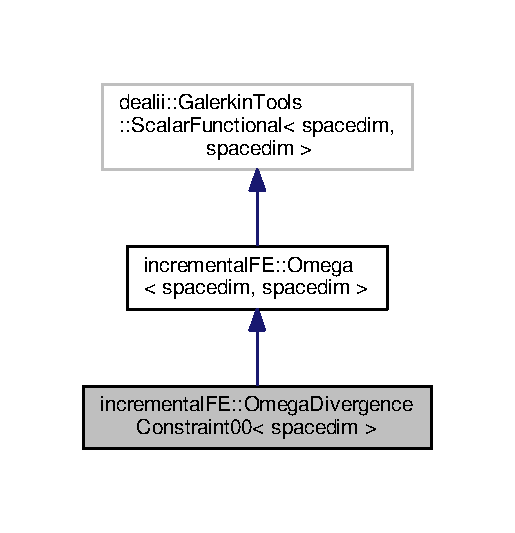
\includegraphics[width=264pt]{classincremental_f_e_1_1_omega_divergence_constraint00__inherit__graph}
\end{center}
\end{figure}


Collaboration diagram for incremental\+FE\+::Omega\+Divergence\+Constraint00$<$ spacedim $>$\+:\nopagebreak
\begin{figure}[H]
\begin{center}
\leavevmode
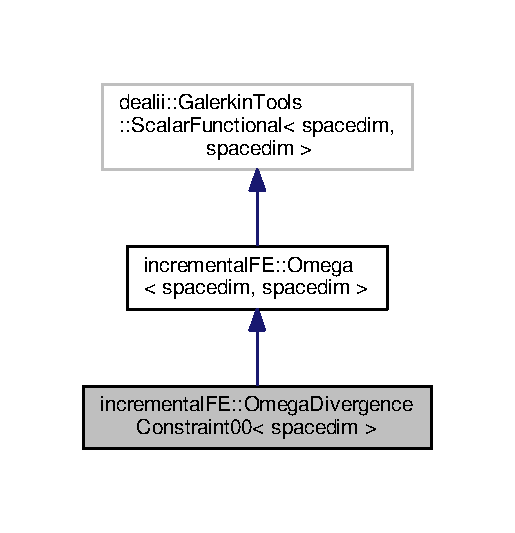
\includegraphics[width=264pt]{classincremental_f_e_1_1_omega_divergence_constraint00__coll__graph}
\end{center}
\end{figure}
\doxysubsection*{Public Member Functions}
\begin{DoxyCompactItemize}
\item 
\mbox{\hyperlink{classincremental_f_e_1_1_omega_divergence_constraint00_a34e18a491023a4e842d2e44ecff7a455}{Omega\+Divergence\+Constraint00}} (const std\+::vector$<$ dealii\+::\+Galerkin\+Tools\+::\+Dependent\+Field$<$ spacedim, spacedim $>$$>$ e\+\_\+omega, const std\+::set$<$ \textbf{ dealii\+::types\+::material\+\_\+id} $>$ domain\+\_\+of\+\_\+integration, const dealii\+::\+Quadrature$<$ spacedim $>$ quadrature, \mbox{\hyperlink{classincremental_f_e_1_1_global_data_incremental_f_e}{Global\+Data\+Incremental\+FE}}$<$ spacedim $>$ \&\mbox{\hyperlink{classincremental_f_e_1_1_omega_3_01spacedim_00_01spacedim_01_4_afffe781a5a2032ec003032adc78e1bf3}{global\+\_\+data}}, const unsigned int \mbox{\hyperlink{classincremental_f_e_1_1_omega_3_01spacedim_00_01spacedim_01_4_a6c95d57122261e8a2e26d3818251bc9b}{method}}, const double \mbox{\hyperlink{classincremental_f_e_1_1_omega_3_01spacedim_00_01spacedim_01_4_ad881c36804cc027c301f4f069756c2db}{alpha}}=0.\+0)
\item 
bool \mbox{\hyperlink{classincremental_f_e_1_1_omega_divergence_constraint00_abf4f1c8217a266dd3afec26d140759b5}{get\+\_\+values\+\_\+and\+\_\+derivatives}} (const \textbf{ dealii\+::\+Vector}$<$ double $>$ \&\textbf{ values}, const double, const dealii\+::\+Point$<$ spacedim $>$ \&, double \&omega, \textbf{ dealii\+::\+Vector}$<$ double $>$ \&d\+\_\+omega, dealii\+::\+Full\+Matrix$<$ double $>$ \&d2\+\_\+omega, const std\+::tuple$<$ bool, bool, bool $>$ requested\+\_\+quantities, const bool) const
\end{DoxyCompactItemize}
\doxysubsection*{Additional Inherited Members}


\doxysubsection{Detailed Description}
\subsubsection*{template$<$unsigned int spacedim$>$\newline
class incremental\+F\+E\+::\+Omega\+Divergence\+Constraint00$<$ spacedim $>$}

Class defining a domain related scalar functional with the integrand

$ \omega^\Omega = -\mu ( \nabla \cdot \dot{\boldsymbol{I}} + \dot{c} ) $

where $\mu$ is a Lagrangian multiplier, $c$ is the species concentration and $\dot{\boldsymbol{I}}$ the corresponding flux.

Ordering of quantities in \textbf{ Scalar\+Functional$<$spacedim, spacedim$>$\+::e\+\_\+omega} \+:~\newline
\mbox{[}0\mbox{]} $\nabla \boldsymbol{I}$~\newline
 \mbox{[}1\mbox{]} $c$~\newline
 \mbox{[}2\mbox{]} $\mu$ 

\doxysubsection{Constructor \& Destructor Documentation}
\mbox{\Hypertarget{classincremental_f_e_1_1_omega_divergence_constraint00_a34e18a491023a4e842d2e44ecff7a455}\label{classincremental_f_e_1_1_omega_divergence_constraint00_a34e18a491023a4e842d2e44ecff7a455}} 
\index{incrementalFE::OmegaDivergenceConstraint00$<$ spacedim $>$@{incrementalFE::OmegaDivergenceConstraint00$<$ spacedim $>$}!OmegaDivergenceConstraint00@{OmegaDivergenceConstraint00}}
\index{OmegaDivergenceConstraint00@{OmegaDivergenceConstraint00}!incrementalFE::OmegaDivergenceConstraint00$<$ spacedim $>$@{incrementalFE::OmegaDivergenceConstraint00$<$ spacedim $>$}}
\doxysubsubsection{\texorpdfstring{OmegaDivergenceConstraint00()}{OmegaDivergenceConstraint00()}}
{\footnotesize\ttfamily template$<$unsigned int spacedim$>$ \\
\mbox{\hyperlink{classincremental_f_e_1_1_omega_divergence_constraint00}{incremental\+F\+E\+::\+Omega\+Divergence\+Constraint00}}$<$ spacedim $>$\+::\mbox{\hyperlink{classincremental_f_e_1_1_omega_divergence_constraint00}{Omega\+Divergence\+Constraint00}} (\begin{DoxyParamCaption}\item[{const std\+::vector$<$ dealii\+::\+Galerkin\+Tools\+::\+Dependent\+Field$<$ spacedim, spacedim $>$$>$}]{e\+\_\+omega,  }\item[{const std\+::set$<$ \textbf{ dealii\+::types\+::material\+\_\+id} $>$}]{domain\+\_\+of\+\_\+integration,  }\item[{const dealii\+::\+Quadrature$<$ spacedim $>$}]{quadrature,  }\item[{\mbox{\hyperlink{classincremental_f_e_1_1_global_data_incremental_f_e}{Global\+Data\+Incremental\+FE}}$<$ spacedim $>$ \&}]{global\+\_\+data,  }\item[{const unsigned int}]{method,  }\item[{const double}]{alpha = {\ttfamily 0.0} }\end{DoxyParamCaption})\hspace{0.3cm}{\ttfamily [inline]}}

Constructor


\begin{DoxyParams}[1]{Parameters}
\mbox{\texttt{ in}}  & {\em e\+\_\+omega} & \textbf{ Scalar\+Functional$<$spacedim, spacedim$>$\+::e\+\_\+omega}\\
\hline
\mbox{\texttt{ in}}  & {\em domain\+\_\+of\+\_\+integration} & \textbf{ Scalar\+Functional$<$spacedim, spacedim$>$\+::domain\+\_\+of\+\_\+integration}\\
\hline
\mbox{\texttt{ in}}  & {\em quadrature} & \textbf{ Scalar\+Functional$<$spacedim, spacedim$>$\+::quadrature}\\
\hline
\mbox{\texttt{ in}}  & {\em global\+\_\+data} & \mbox{\hyperlink{classincremental_f_e_1_1_omega_3_01spacedim_00_01spacedim_01_4_afffe781a5a2032ec003032adc78e1bf3}{Omega$<$spacedim, spacedim$>$\+::global\+\_\+data}}\\
\hline
\mbox{\texttt{ in}}  & {\em method} & \mbox{\hyperlink{classincremental_f_e_1_1_omega_3_01spacedim_00_01spacedim_01_4_a6c95d57122261e8a2e26d3818251bc9b}{Omega$<$spacedim, spacedim$>$\+::method}}\\
\hline
\mbox{\texttt{ in}}  & {\em alpha} & \mbox{\hyperlink{classincremental_f_e_1_1_omega_3_01spacedim_00_01spacedim_01_4_ad881c36804cc027c301f4f069756c2db}{Omega$<$spacedim, spacedim$>$\+::alpha}} \\
\hline
\end{DoxyParams}


\doxysubsection{Member Function Documentation}
\mbox{\Hypertarget{classincremental_f_e_1_1_omega_divergence_constraint00_abf4f1c8217a266dd3afec26d140759b5}\label{classincremental_f_e_1_1_omega_divergence_constraint00_abf4f1c8217a266dd3afec26d140759b5}} 
\index{incrementalFE::OmegaDivergenceConstraint00$<$ spacedim $>$@{incrementalFE::OmegaDivergenceConstraint00$<$ spacedim $>$}!get\_values\_and\_derivatives@{get\_values\_and\_derivatives}}
\index{get\_values\_and\_derivatives@{get\_values\_and\_derivatives}!incrementalFE::OmegaDivergenceConstraint00$<$ spacedim $>$@{incrementalFE::OmegaDivergenceConstraint00$<$ spacedim $>$}}
\doxysubsubsection{\texorpdfstring{get\_values\_and\_derivatives()}{get\_values\_and\_derivatives()}}
{\footnotesize\ttfamily template$<$unsigned int spacedim$>$ \\
bool \mbox{\hyperlink{classincremental_f_e_1_1_omega_divergence_constraint00}{incremental\+F\+E\+::\+Omega\+Divergence\+Constraint00}}$<$ spacedim $>$\+::get\+\_\+values\+\_\+and\+\_\+derivatives (\begin{DoxyParamCaption}\item[{const \textbf{ dealii\+::\+Vector}$<$ double $>$ \&}]{values,  }\item[{const double}]{,  }\item[{const dealii\+::\+Point$<$ spacedim $>$ \&}]{,  }\item[{double \&}]{omega,  }\item[{\textbf{ dealii\+::\+Vector}$<$ double $>$ \&}]{d\+\_\+omega,  }\item[{dealii\+::\+Full\+Matrix$<$ double $>$ \&}]{d2\+\_\+omega,  }\item[{const std\+::tuple$<$ bool, bool, bool $>$}]{requested\+\_\+quantities,  }\item[{const bool}]{ }\end{DoxyParamCaption}) const\hspace{0.3cm}{\ttfamily [inline]}, {\ttfamily [virtual]}}

\begin{DoxySeeAlso}{See also}
\mbox{\hyperlink{classincremental_f_e_1_1_omega_3_01spacedim_00_01spacedim_01_4_a40131354ef0a28ca48a0e6c9ed33aa33}{Omega$<$spacedim, spacedim$>$\+::get\+\_\+values\+\_\+and\+\_\+derivatives()}} 
\end{DoxySeeAlso}


Implements \mbox{\hyperlink{classincremental_f_e_1_1_omega_3_01spacedim_00_01spacedim_01_4_a40131354ef0a28ca48a0e6c9ed33aa33}{incremental\+F\+E\+::\+Omega$<$ spacedim, spacedim $>$}}.



The documentation for this class was generated from the following file\+:\begin{DoxyCompactItemize}
\item 
/home/sst/code/\+Incremental\+F\+E/\+Incremental\+F\+E/include/incremental\+\_\+fe/scalar\+\_\+functionals/\mbox{\hyperlink{omega__lib_8h}{omega\+\_\+lib.\+h}}\end{DoxyCompactItemize}

\hypertarget{classincremental_f_e_1_1_omega_dual_butler_volmer00}{}\section{incremental\+FE\+:\+:Omega\+Dual\+Butler\+Volmer00$<$ spacedim $>$ Class Template Reference}
\label{classincremental_f_e_1_1_omega_dual_butler_volmer00}\index{incremental\+F\+E\+::\+Omega\+Dual\+Butler\+Volmer00$<$ spacedim $>$@{incremental\+F\+E\+::\+Omega\+Dual\+Butler\+Volmer00$<$ spacedim $>$}}


{\ttfamily \#include $<$omega\+\_\+lib.\+h$>$}



Inheritance diagram for incremental\+FE\+:\+:Omega\+Dual\+Butler\+Volmer00$<$ spacedim $>$\+:\nopagebreak
\begin{figure}[H]
\begin{center}
\leavevmode
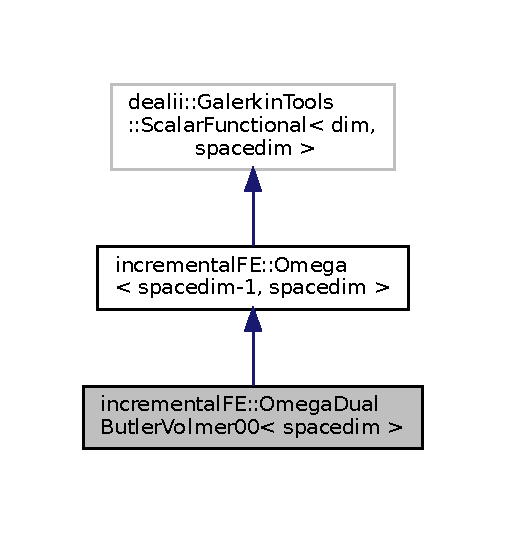
\includegraphics[width=223pt]{classincremental_f_e_1_1_omega_dual_butler_volmer00__inherit__graph}
\end{center}
\end{figure}


Collaboration diagram for incremental\+FE\+:\+:Omega\+Dual\+Butler\+Volmer00$<$ spacedim $>$\+:\nopagebreak
\begin{figure}[H]
\begin{center}
\leavevmode
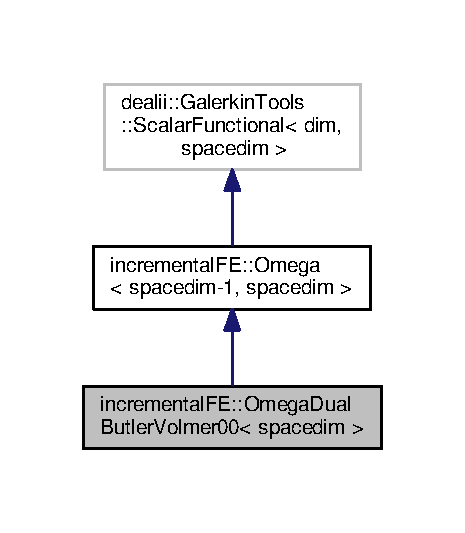
\includegraphics[width=223pt]{classincremental_f_e_1_1_omega_dual_butler_volmer00__coll__graph}
\end{center}
\end{figure}
\subsection*{Public Member Functions}
\begin{DoxyCompactItemize}
\item 
\hyperlink{classincremental_f_e_1_1_omega_dual_butler_volmer00_a4bc64f76770f63e634478f19798d9d27}{Omega\+Dual\+Butler\+Volmer00} (const std\+::vector$<$ dealii\+::\+Galerkin\+Tools\+::\+Dependent\+Field$<$ spacedim-\/1, spacedim $>$$>$ e\+\_\+sigma, const std\+::set$<$ {\bf dealii\+::types\+::material\+\_\+id} $>$ domain\+\_\+of\+\_\+integration, const dealii\+::\+Quadrature$<$ spacedim-\/1 $>$ quadrature, \hyperlink{classincremental_f_e_1_1_global_data_incremental_f_e}{Global\+Data\+Incremental\+FE}$<$ spacedim $>$ \&\hyperlink{classincremental_f_e_1_1_omega_abd23d288a7a4a43f9b528be968cd2113}{global\+\_\+data}, const double \hyperlink{classincremental_f_e_1_1_omega_dual_butler_volmer00_a37608eb032b6e88dd8c9a7d0f553a0bd}{I\+\_\+0}, const double \hyperlink{classincremental_f_e_1_1_omega_dual_butler_volmer00_a8823655ea8aa9eb5668a64c6ee7bf4be}{beta}, const double \hyperlink{classincremental_f_e_1_1_omega_dual_butler_volmer00_a2f32c4f92c11646ed2f6741977d9833f}{RT}, const double \hyperlink{classincremental_f_e_1_1_omega_dual_butler_volmer00_abdc57ace8b842d20ea8f8941b948db41}{threshold}, const unsigned int \hyperlink{classincremental_f_e_1_1_omega_a7600d263ebf98129629e44fa67e8a58c}{method}, const double \hyperlink{classincremental_f_e_1_1_omega_a891688560ec0ad8dc5a0058a7b400269}{alpha}=0.\+0)
\item 
bool \hyperlink{classincremental_f_e_1_1_omega_dual_butler_volmer00_af5cc5ae73af89acdea968203cb29e415}{get\+\_\+values\+\_\+and\+\_\+derivatives} (const {\bf dealii\+::\+Vector}$<$ double $>$ \&{\bf values}, const double, const dealii\+::\+Point$<$ spacedim $>$ \&, const dealii\+::\+Tensor$<$ 1, spacedim $>$ \&, double \&omega, {\bf dealii\+::\+Vector}$<$ double $>$ \&d\+\_\+omega, dealii\+::\+Full\+Matrix$<$ double $>$ \&d2\+\_\+omega, const std\+::tuple$<$ bool, bool, bool $>$ requested\+\_\+quantities, const bool) const 
\end{DoxyCompactItemize}
\subsection*{Private Attributes}
\begin{DoxyCompactItemize}
\item 
const double \hyperlink{classincremental_f_e_1_1_omega_dual_butler_volmer00_a37608eb032b6e88dd8c9a7d0f553a0bd}{I\+\_\+0}
\item 
const double \hyperlink{classincremental_f_e_1_1_omega_dual_butler_volmer00_a8823655ea8aa9eb5668a64c6ee7bf4be}{beta}
\item 
const double \hyperlink{classincremental_f_e_1_1_omega_dual_butler_volmer00_a2f32c4f92c11646ed2f6741977d9833f}{RT}
\item 
const double \hyperlink{classincremental_f_e_1_1_omega_dual_butler_volmer00_abdc57ace8b842d20ea8f8941b948db41}{threshold}
\end{DoxyCompactItemize}
\subsection*{Additional Inherited Members}


\subsection{Detailed Description}
\subsubsection*{template$<$unsigned int spacedim$>$\\*
class incremental\+F\+E\+::\+Omega\+Dual\+Butler\+Volmer00$<$ spacedim $>$}

Class defining an interface related Butler-\/\+Volmer type scalar functional with the integrand

$ h^\Sigma_\tau = -I_0\left[ \dfrac{1}{1-\beta} \exp\left( - \dfrac{1-\beta}{RT} \Delta \eta \right) + \dfrac{1}{\beta} \exp\left( \dfrac{\beta}{RT} \Delta \eta \right) \right] $

where $I_0$ is related to the exchange current density $i_0$ by $I_0 = i_0 \cdot RT / F $, $\beta$ is the symmetry factor, and $\Delta \eta$ the thermodynamic driving force.

Ordering of quantities in {\bf Scalar\+Functional\+::e\+\_\+sigma} \+:~\newline
\mbox{[}0\mbox{]} $\Delta \eta$ 

\subsection{Constructor \& Destructor Documentation}
\index{incremental\+F\+E\+::\+Omega\+Dual\+Butler\+Volmer00@{incremental\+F\+E\+::\+Omega\+Dual\+Butler\+Volmer00}!Omega\+Dual\+Butler\+Volmer00@{Omega\+Dual\+Butler\+Volmer00}}
\index{Omega\+Dual\+Butler\+Volmer00@{Omega\+Dual\+Butler\+Volmer00}!incremental\+F\+E\+::\+Omega\+Dual\+Butler\+Volmer00@{incremental\+F\+E\+::\+Omega\+Dual\+Butler\+Volmer00}}
\subsubsection[{\texorpdfstring{Omega\+Dual\+Butler\+Volmer00(const std\+::vector$<$ dealii\+::\+Galerkin\+Tools\+::\+Dependent\+Field$<$ spacedim-\/1, spacedim $>$$>$ e\+\_\+sigma, const std\+::set$<$ dealii\+::types\+::material\+\_\+id $>$ domain\+\_\+of\+\_\+integration, const dealii\+::\+Quadrature$<$ spacedim-\/1 $>$ quadrature, Global\+Data\+Incremental\+F\+E$<$ spacedim $>$ \&global\+\_\+data, const double I\+\_\+0, const double beta, const double R\+T, const double threshold, const unsigned int method, const double alpha=0.\+0)}{OmegaDualButlerVolmer00(const std::vector< dealii::GalerkinTools::DependentField< spacedim-1, spacedim >> e_sigma, const std::set< dealii::types::material_id > domain_of_integration, const dealii::Quadrature< spacedim-1 > quadrature, GlobalDataIncrementalFE< spacedim > &global_data, const double I_0, const double beta, const double RT, const double threshold, const unsigned int method, const double alpha=0.0)}}]{\setlength{\rightskip}{0pt plus 5cm}template$<$unsigned int spacedim$>$ {\bf incremental\+F\+E\+::\+Omega\+Dual\+Butler\+Volmer00}$<$ spacedim $>$\+::{\bf Omega\+Dual\+Butler\+Volmer00} (
\begin{DoxyParamCaption}
\item[{const std\+::vector$<$ dealii\+::\+Galerkin\+Tools\+::\+Dependent\+Field$<$ spacedim-\/1, spacedim $>$$>$}]{e\+\_\+sigma, }
\item[{const std\+::set$<$ {\bf dealii\+::types\+::material\+\_\+id} $>$}]{domain\+\_\+of\+\_\+integration, }
\item[{const dealii\+::\+Quadrature$<$ spacedim-\/1 $>$}]{quadrature, }
\item[{{\bf Global\+Data\+Incremental\+FE}$<$ spacedim $>$ \&}]{global\+\_\+data, }
\item[{const double}]{I\+\_\+0, }
\item[{const double}]{beta, }
\item[{const double}]{RT, }
\item[{const double}]{threshold, }
\item[{const unsigned int}]{method, }
\item[{const double}]{alpha = {\ttfamily 0.0}}
\end{DoxyParamCaption}
)\hspace{0.3cm}{\ttfamily [inline]}}\hypertarget{classincremental_f_e_1_1_omega_dual_butler_volmer00_a4bc64f76770f63e634478f19798d9d27}{}\label{classincremental_f_e_1_1_omega_dual_butler_volmer00_a4bc64f76770f63e634478f19798d9d27}
Constructor


\begin{DoxyParams}[1]{Parameters}
\mbox{\tt in}  & {\em e\+\_\+sigma} & {\bf Scalar\+Functional\+::e\+\_\+sigma}\\
\hline
\mbox{\tt in}  & {\em domain\+\_\+of\+\_\+integration} & {\bf Scalar\+Functional\+::domain\+\_\+of\+\_\+integration}\\
\hline
\mbox{\tt in}  & {\em quadrature} & {\bf Scalar\+Functional\+::quadrature}\\
\hline
\mbox{\tt in}  & {\em global\+\_\+data} & \hyperlink{classincremental_f_e_1_1_omega_abd23d288a7a4a43f9b528be968cd2113}{Omega\+::global\+\_\+data}\\
\hline
\mbox{\tt in}  & {\em I\+\_\+0} & \hyperlink{classincremental_f_e_1_1_omega_dual_butler_volmer00_a37608eb032b6e88dd8c9a7d0f553a0bd}{Omega\+Dual\+Butler\+Volmer00\+::\+I\+\_\+0}\\
\hline
\mbox{\tt in}  & {\em beta} & \hyperlink{classincremental_f_e_1_1_omega_dual_butler_volmer00_a8823655ea8aa9eb5668a64c6ee7bf4be}{Omega\+Dual\+Butler\+Volmer00\+::beta}\\
\hline
\mbox{\tt in}  & {\em RT} & \hyperlink{classincremental_f_e_1_1_omega_dual_butler_volmer00_a2f32c4f92c11646ed2f6741977d9833f}{Omega\+Dual\+Butler\+Volmer00\+::\+RT}\\
\hline
\mbox{\tt in}  & {\em threshold} & \hyperlink{classincremental_f_e_1_1_omega_dual_butler_volmer00_abdc57ace8b842d20ea8f8941b948db41}{Omega\+Dual\+Butler\+Volmer00\+::threshold}\\
\hline
\mbox{\tt in}  & {\em method} & \hyperlink{classincremental_f_e_1_1_omega_a7600d263ebf98129629e44fa67e8a58c}{Omega\+::method}\\
\hline
\mbox{\tt in}  & {\em alpha} & \hyperlink{classincremental_f_e_1_1_omega_a891688560ec0ad8dc5a0058a7b400269}{Omega\+::alpha} \\
\hline
\end{DoxyParams}


\subsection{Member Function Documentation}
\index{incremental\+F\+E\+::\+Omega\+Dual\+Butler\+Volmer00@{incremental\+F\+E\+::\+Omega\+Dual\+Butler\+Volmer00}!get\+\_\+values\+\_\+and\+\_\+derivatives@{get\+\_\+values\+\_\+and\+\_\+derivatives}}
\index{get\+\_\+values\+\_\+and\+\_\+derivatives@{get\+\_\+values\+\_\+and\+\_\+derivatives}!incremental\+F\+E\+::\+Omega\+Dual\+Butler\+Volmer00@{incremental\+F\+E\+::\+Omega\+Dual\+Butler\+Volmer00}}
\subsubsection[{\texorpdfstring{get\+\_\+values\+\_\+and\+\_\+derivatives(const dealii\+::\+Vector$<$ double $>$ \&values, const double, const dealii\+::\+Point$<$ spacedim $>$ \&, const dealii\+::\+Tensor$<$ 1, spacedim $>$ \&, double \&omega, dealii\+::\+Vector$<$ double $>$ \&d\+\_\+omega, dealii\+::\+Full\+Matrix$<$ double $>$ \&d2\+\_\+omega, const std\+::tuple$<$ bool, bool, bool $>$ requested\+\_\+quantities, const bool) const }{get_values_and_derivatives(const dealii::Vector< double > &values, const double, const dealii::Point< spacedim > &, const dealii::Tensor< 1, spacedim > &, double &omega, dealii::Vector< double > &d_omega, dealii::FullMatrix< double > &d2_omega, const std::tuple< bool, bool, bool > requested_quantities, const bool) const }}]{\setlength{\rightskip}{0pt plus 5cm}template$<$unsigned int spacedim$>$ bool {\bf incremental\+F\+E\+::\+Omega\+Dual\+Butler\+Volmer00}$<$ spacedim $>$\+::get\+\_\+values\+\_\+and\+\_\+derivatives (
\begin{DoxyParamCaption}
\item[{const {\bf dealii\+::\+Vector}$<$ double $>$ \&}]{values, }
\item[{const double}]{, }
\item[{const dealii\+::\+Point$<$ spacedim $>$ \&}]{, }
\item[{const dealii\+::\+Tensor$<$ 1, spacedim $>$ \&}]{, }
\item[{double \&}]{omega, }
\item[{{\bf dealii\+::\+Vector}$<$ double $>$ \&}]{d\+\_\+omega, }
\item[{dealii\+::\+Full\+Matrix$<$ double $>$ \&}]{d2\+\_\+omega, }
\item[{const std\+::tuple$<$ bool, bool, bool $>$}]{requested\+\_\+quantities, }
\item[{const bool}]{}
\end{DoxyParamCaption}
) const\hspace{0.3cm}{\ttfamily [inline]}, {\ttfamily [virtual]}}\hypertarget{classincremental_f_e_1_1_omega_dual_butler_volmer00_af5cc5ae73af89acdea968203cb29e415}{}\label{classincremental_f_e_1_1_omega_dual_butler_volmer00_af5cc5ae73af89acdea968203cb29e415}
\begin{DoxySeeAlso}{See also}
\hyperlink{classincremental_f_e_1_1_omega_a2f35d862aefa11151de5b7c7411e45df}{Omega\+::get\+\_\+values\+\_\+and\+\_\+derivatives()} 
\end{DoxySeeAlso}


Implements \hyperlink{classincremental_f_e_1_1_omega_a2f35d862aefa11151de5b7c7411e45df}{incremental\+F\+E\+::\+Omega$<$ spacedim-\/1, spacedim $>$}.



\subsection{Member Data Documentation}
\index{incremental\+F\+E\+::\+Omega\+Dual\+Butler\+Volmer00@{incremental\+F\+E\+::\+Omega\+Dual\+Butler\+Volmer00}!beta@{beta}}
\index{beta@{beta}!incremental\+F\+E\+::\+Omega\+Dual\+Butler\+Volmer00@{incremental\+F\+E\+::\+Omega\+Dual\+Butler\+Volmer00}}
\subsubsection[{\texorpdfstring{beta}{beta}}]{\setlength{\rightskip}{0pt plus 5cm}template$<$unsigned int spacedim$>$ const double {\bf incremental\+F\+E\+::\+Omega\+Dual\+Butler\+Volmer00}$<$ spacedim $>$\+::beta\hspace{0.3cm}{\ttfamily [private]}}\hypertarget{classincremental_f_e_1_1_omega_dual_butler_volmer00_a8823655ea8aa9eb5668a64c6ee7bf4be}{}\label{classincremental_f_e_1_1_omega_dual_butler_volmer00_a8823655ea8aa9eb5668a64c6ee7bf4be}
parameter $\beta$ \index{incremental\+F\+E\+::\+Omega\+Dual\+Butler\+Volmer00@{incremental\+F\+E\+::\+Omega\+Dual\+Butler\+Volmer00}!I\+\_\+0@{I\+\_\+0}}
\index{I\+\_\+0@{I\+\_\+0}!incremental\+F\+E\+::\+Omega\+Dual\+Butler\+Volmer00@{incremental\+F\+E\+::\+Omega\+Dual\+Butler\+Volmer00}}
\subsubsection[{\texorpdfstring{I\+\_\+0}{I_0}}]{\setlength{\rightskip}{0pt plus 5cm}template$<$unsigned int spacedim$>$ const double {\bf incremental\+F\+E\+::\+Omega\+Dual\+Butler\+Volmer00}$<$ spacedim $>$\+::I\+\_\+0\hspace{0.3cm}{\ttfamily [private]}}\hypertarget{classincremental_f_e_1_1_omega_dual_butler_volmer00_a37608eb032b6e88dd8c9a7d0f553a0bd}{}\label{classincremental_f_e_1_1_omega_dual_butler_volmer00_a37608eb032b6e88dd8c9a7d0f553a0bd}
parameter $I_0$ \index{incremental\+F\+E\+::\+Omega\+Dual\+Butler\+Volmer00@{incremental\+F\+E\+::\+Omega\+Dual\+Butler\+Volmer00}!RT@{RT}}
\index{RT@{RT}!incremental\+F\+E\+::\+Omega\+Dual\+Butler\+Volmer00@{incremental\+F\+E\+::\+Omega\+Dual\+Butler\+Volmer00}}
\subsubsection[{\texorpdfstring{RT}{RT}}]{\setlength{\rightskip}{0pt plus 5cm}template$<$unsigned int spacedim$>$ const double {\bf incremental\+F\+E\+::\+Omega\+Dual\+Butler\+Volmer00}$<$ spacedim $>$\+::RT\hspace{0.3cm}{\ttfamily [private]}}\hypertarget{classincremental_f_e_1_1_omega_dual_butler_volmer00_a2f32c4f92c11646ed2f6741977d9833f}{}\label{classincremental_f_e_1_1_omega_dual_butler_volmer00_a2f32c4f92c11646ed2f6741977d9833f}
$RT$ \index{incremental\+F\+E\+::\+Omega\+Dual\+Butler\+Volmer00@{incremental\+F\+E\+::\+Omega\+Dual\+Butler\+Volmer00}!threshold@{threshold}}
\index{threshold@{threshold}!incremental\+F\+E\+::\+Omega\+Dual\+Butler\+Volmer00@{incremental\+F\+E\+::\+Omega\+Dual\+Butler\+Volmer00}}
\subsubsection[{\texorpdfstring{threshold}{threshold}}]{\setlength{\rightskip}{0pt plus 5cm}template$<$unsigned int spacedim$>$ const double {\bf incremental\+F\+E\+::\+Omega\+Dual\+Butler\+Volmer00}$<$ spacedim $>$\+::threshold\hspace{0.3cm}{\ttfamily [private]}}\hypertarget{classincremental_f_e_1_1_omega_dual_butler_volmer00_abdc57ace8b842d20ea8f8941b948db41}{}\label{classincremental_f_e_1_1_omega_dual_butler_volmer00_abdc57ace8b842d20ea8f8941b948db41}
Threshold parameter $\Delta \eta^\mathrm{th}/RT$. If $|\Delta \eta/RT| > \Delta \eta^\mathrm{th}/RT$, the potential is continued by a quadratic function in order to avoid numerical issues related to large values of the exponential function. 

The documentation for this class was generated from the following file\+:\begin{DoxyCompactItemize}
\item 
/home/sst/code/\+Incremental\+F\+E/\+Incremental\+F\+E/include/incremental\+\_\+fe/scalar\+\_\+functionals/\hyperlink{omega__lib_8h}{omega\+\_\+lib.\+h}\end{DoxyCompactItemize}

\hypertarget{classincremental_f_e_1_1_omega_dual_flux_dissipation00}{}\doxysection{incremental\+FE\+::Omega\+Dual\+Flux\+Dissipation00$<$ spacedim $>$ Class Template Reference}
\label{classincremental_f_e_1_1_omega_dual_flux_dissipation00}\index{incrementalFE::OmegaDualFluxDissipation00$<$ spacedim $>$@{incrementalFE::OmegaDualFluxDissipation00$<$ spacedim $>$}}


{\ttfamily \#include $<$omega\+\_\+lib.\+h$>$}



Inheritance diagram for incremental\+FE\+::Omega\+Dual\+Flux\+Dissipation00$<$ spacedim $>$\+:\nopagebreak
\begin{figure}[H]
\begin{center}
\leavevmode
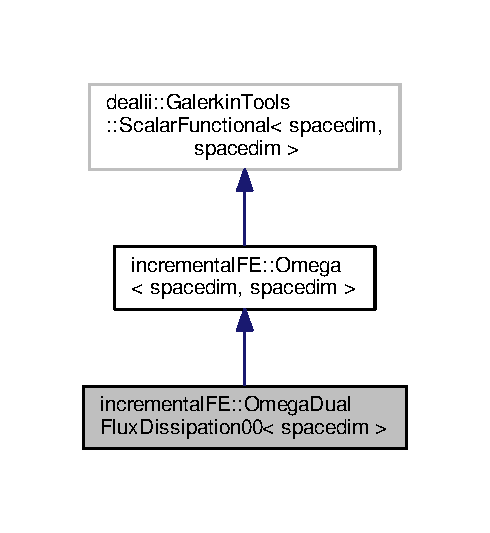
\includegraphics[width=254pt]{classincremental_f_e_1_1_omega_dual_flux_dissipation00__inherit__graph}
\end{center}
\end{figure}


Collaboration diagram for incremental\+FE\+::Omega\+Dual\+Flux\+Dissipation00$<$ spacedim $>$\+:\nopagebreak
\begin{figure}[H]
\begin{center}
\leavevmode
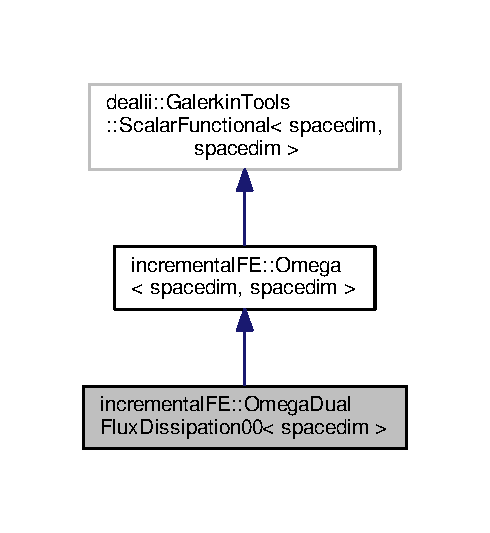
\includegraphics[width=254pt]{classincremental_f_e_1_1_omega_dual_flux_dissipation00__coll__graph}
\end{center}
\end{figure}
\doxysubsection*{Public Member Functions}
\begin{DoxyCompactItemize}
\item 
\mbox{\hyperlink{classincremental_f_e_1_1_omega_dual_flux_dissipation00_a4f1fb84afb78bd1718ba36c63fe3a22b}{Omega\+Dual\+Flux\+Dissipation00}} (const std\+::vector$<$ dealii\+::\+Galerkin\+Tools\+::\+Dependent\+Field$<$ spacedim, spacedim $>$$>$ e\+\_\+omega, const std\+::set$<$ \textbf{ dealii\+::types\+::material\+\_\+id} $>$ domain\+\_\+of\+\_\+integration, const dealii\+::\+Quadrature$<$ spacedim $>$ quadrature, \mbox{\hyperlink{classincremental_f_e_1_1_global_data_incremental_f_e}{Global\+Data\+Incremental\+FE}}$<$ spacedim $>$ \&\mbox{\hyperlink{classincremental_f_e_1_1_omega_3_01spacedim_00_01spacedim_01_4_afffe781a5a2032ec003032adc78e1bf3}{global\+\_\+data}}, const double \mbox{\hyperlink{classincremental_f_e_1_1_omega_dual_flux_dissipation00_a922910cdc92b29321d37bf46dc50f41a}{D}}, const unsigned int \mbox{\hyperlink{classincremental_f_e_1_1_omega_3_01spacedim_00_01spacedim_01_4_a6c95d57122261e8a2e26d3818251bc9b}{method}}, const double \mbox{\hyperlink{classincremental_f_e_1_1_omega_3_01spacedim_00_01spacedim_01_4_ad881c36804cc027c301f4f069756c2db}{alpha}}=0.\+0)
\item 
bool \mbox{\hyperlink{classincremental_f_e_1_1_omega_dual_flux_dissipation00_a74ae73b7e52de1c084992628ab2a6328}{get\+\_\+values\+\_\+and\+\_\+derivatives}} (const \textbf{ dealii\+::\+Vector}$<$ double $>$ \&\textbf{ values}, const double, const dealii\+::\+Point$<$ spacedim $>$ \&, double \&omega, \textbf{ dealii\+::\+Vector}$<$ double $>$ \&d\+\_\+omega, dealii\+::\+Full\+Matrix$<$ double $>$ \&d2\+\_\+omega, const std\+::tuple$<$ bool, bool, bool $>$ requested\+\_\+quantities, const bool compute\+\_\+dq) const
\end{DoxyCompactItemize}
\doxysubsection*{Private Attributes}
\begin{DoxyCompactItemize}
\item 
const double \mbox{\hyperlink{classincremental_f_e_1_1_omega_dual_flux_dissipation00_a922910cdc92b29321d37bf46dc50f41a}{D}}
\end{DoxyCompactItemize}
\doxysubsection*{Additional Inherited Members}


\doxysubsection{Detailed Description}
\subsubsection*{template$<$unsigned int spacedim$>$\newline
class incremental\+F\+E\+::\+Omega\+Dual\+Flux\+Dissipation00$<$ spacedim $>$}

Class defining a domain related scalar functional with the integrand

$ h^\Omega_\rho = -\dfrac{D c}{2} \boldsymbol{E} \cdot \boldsymbol{E} $,

where $c$ is the species concentration and $\boldsymbol{E}$ the driving force vector for the corresponding species flux.

The \char`\"{}mobility\char`\"{} $D$ is related to the usual \char`\"{}diffusion constant\char`\"{} $ \bar D $ by $D = \bar D/(RT)$. Moreover, it is related to the electrical mobility $\mu$ by $ D = \mu n/F$, where $n$ is the charge per molecule of the mobile species in multiples of the elementary charge and $F$ Faraday\textquotesingle{}s constant.

Ordering of quantities in \textbf{ Scalar\+Functional$<$spacedim, spacedim$>$\+::e\+\_\+omega} \+:~\newline
\mbox{[}0\mbox{]} $E_x$~\newline
 \mbox{[}1\mbox{]} $E_y$~\newline
 \mbox{[}2\mbox{]} $E_z$~\newline
 \mbox{[}3\mbox{]} $c$ 

\doxysubsection{Constructor \& Destructor Documentation}
\mbox{\Hypertarget{classincremental_f_e_1_1_omega_dual_flux_dissipation00_a4f1fb84afb78bd1718ba36c63fe3a22b}\label{classincremental_f_e_1_1_omega_dual_flux_dissipation00_a4f1fb84afb78bd1718ba36c63fe3a22b}} 
\index{incrementalFE::OmegaDualFluxDissipation00$<$ spacedim $>$@{incrementalFE::OmegaDualFluxDissipation00$<$ spacedim $>$}!OmegaDualFluxDissipation00@{OmegaDualFluxDissipation00}}
\index{OmegaDualFluxDissipation00@{OmegaDualFluxDissipation00}!incrementalFE::OmegaDualFluxDissipation00$<$ spacedim $>$@{incrementalFE::OmegaDualFluxDissipation00$<$ spacedim $>$}}
\doxysubsubsection{\texorpdfstring{OmegaDualFluxDissipation00()}{OmegaDualFluxDissipation00()}}
{\footnotesize\ttfamily template$<$unsigned int spacedim$>$ \\
\mbox{\hyperlink{classincremental_f_e_1_1_omega_dual_flux_dissipation00}{incremental\+F\+E\+::\+Omega\+Dual\+Flux\+Dissipation00}}$<$ spacedim $>$\+::\mbox{\hyperlink{classincremental_f_e_1_1_omega_dual_flux_dissipation00}{Omega\+Dual\+Flux\+Dissipation00}} (\begin{DoxyParamCaption}\item[{const std\+::vector$<$ dealii\+::\+Galerkin\+Tools\+::\+Dependent\+Field$<$ spacedim, spacedim $>$$>$}]{e\+\_\+omega,  }\item[{const std\+::set$<$ \textbf{ dealii\+::types\+::material\+\_\+id} $>$}]{domain\+\_\+of\+\_\+integration,  }\item[{const dealii\+::\+Quadrature$<$ spacedim $>$}]{quadrature,  }\item[{\mbox{\hyperlink{classincremental_f_e_1_1_global_data_incremental_f_e}{Global\+Data\+Incremental\+FE}}$<$ spacedim $>$ \&}]{global\+\_\+data,  }\item[{const double}]{D,  }\item[{const unsigned int}]{method,  }\item[{const double}]{alpha = {\ttfamily 0.0} }\end{DoxyParamCaption})\hspace{0.3cm}{\ttfamily [inline]}}

Constructor


\begin{DoxyParams}[1]{Parameters}
\mbox{\texttt{ in}}  & {\em e\+\_\+omega} & \textbf{ Scalar\+Functional$<$spacedim, spacedim$>$\+::e\+\_\+omega}\\
\hline
\mbox{\texttt{ in}}  & {\em domain\+\_\+of\+\_\+integration} & \textbf{ Scalar\+Functional$<$spacedim, spacedim$>$\+::domain\+\_\+of\+\_\+integration}\\
\hline
\mbox{\texttt{ in}}  & {\em quadrature} & \textbf{ Scalar\+Functional$<$spacedim, spacedim$>$\+::quadrature}\\
\hline
\mbox{\texttt{ in}}  & {\em global\+\_\+data} & \mbox{\hyperlink{classincremental_f_e_1_1_omega_3_01spacedim_00_01spacedim_01_4_afffe781a5a2032ec003032adc78e1bf3}{Omega$<$spacedim, spacedim$>$\+::global\+\_\+data}}\\
\hline
\mbox{\texttt{ in}}  & {\em D} & \mbox{\hyperlink{classincremental_f_e_1_1_omega_dual_flux_dissipation00_a922910cdc92b29321d37bf46dc50f41a}{Omega\+Dual\+Flux\+Dissipation00\+::D}}\\
\hline
\mbox{\texttt{ in}}  & {\em method} & \mbox{\hyperlink{classincremental_f_e_1_1_omega_3_01spacedim_00_01spacedim_01_4_a6c95d57122261e8a2e26d3818251bc9b}{Omega$<$spacedim, spacedim$>$\+::method}}\\
\hline
\mbox{\texttt{ in}}  & {\em alpha} & \mbox{\hyperlink{classincremental_f_e_1_1_omega_3_01spacedim_00_01spacedim_01_4_ad881c36804cc027c301f4f069756c2db}{Omega$<$spacedim, spacedim$>$\+::alpha}} \\
\hline
\end{DoxyParams}


\doxysubsection{Member Function Documentation}
\mbox{\Hypertarget{classincremental_f_e_1_1_omega_dual_flux_dissipation00_a74ae73b7e52de1c084992628ab2a6328}\label{classincremental_f_e_1_1_omega_dual_flux_dissipation00_a74ae73b7e52de1c084992628ab2a6328}} 
\index{incrementalFE::OmegaDualFluxDissipation00$<$ spacedim $>$@{incrementalFE::OmegaDualFluxDissipation00$<$ spacedim $>$}!get\_values\_and\_derivatives@{get\_values\_and\_derivatives}}
\index{get\_values\_and\_derivatives@{get\_values\_and\_derivatives}!incrementalFE::OmegaDualFluxDissipation00$<$ spacedim $>$@{incrementalFE::OmegaDualFluxDissipation00$<$ spacedim $>$}}
\doxysubsubsection{\texorpdfstring{get\_values\_and\_derivatives()}{get\_values\_and\_derivatives()}}
{\footnotesize\ttfamily template$<$unsigned int spacedim$>$ \\
bool \mbox{\hyperlink{classincremental_f_e_1_1_omega_dual_flux_dissipation00}{incremental\+F\+E\+::\+Omega\+Dual\+Flux\+Dissipation00}}$<$ spacedim $>$\+::get\+\_\+values\+\_\+and\+\_\+derivatives (\begin{DoxyParamCaption}\item[{const \textbf{ dealii\+::\+Vector}$<$ double $>$ \&}]{values,  }\item[{const double}]{,  }\item[{const dealii\+::\+Point$<$ spacedim $>$ \&}]{,  }\item[{double \&}]{omega,  }\item[{\textbf{ dealii\+::\+Vector}$<$ double $>$ \&}]{d\+\_\+omega,  }\item[{dealii\+::\+Full\+Matrix$<$ double $>$ \&}]{d2\+\_\+omega,  }\item[{const std\+::tuple$<$ bool, bool, bool $>$}]{requested\+\_\+quantities,  }\item[{const bool}]{compute\+\_\+dq }\end{DoxyParamCaption}) const\hspace{0.3cm}{\ttfamily [inline]}, {\ttfamily [virtual]}}

\begin{DoxySeeAlso}{See also}
\mbox{\hyperlink{classincremental_f_e_1_1_omega_3_01spacedim_00_01spacedim_01_4_a40131354ef0a28ca48a0e6c9ed33aa33}{Omega$<$spacedim, spacedim$>$\+::get\+\_\+values\+\_\+and\+\_\+derivatives()}} 
\end{DoxySeeAlso}


Implements \mbox{\hyperlink{classincremental_f_e_1_1_omega_3_01spacedim_00_01spacedim_01_4_a40131354ef0a28ca48a0e6c9ed33aa33}{incremental\+F\+E\+::\+Omega$<$ spacedim, spacedim $>$}}.



\doxysubsection{Member Data Documentation}
\mbox{\Hypertarget{classincremental_f_e_1_1_omega_dual_flux_dissipation00_a922910cdc92b29321d37bf46dc50f41a}\label{classincremental_f_e_1_1_omega_dual_flux_dissipation00_a922910cdc92b29321d37bf46dc50f41a}} 
\index{incrementalFE::OmegaDualFluxDissipation00$<$ spacedim $>$@{incrementalFE::OmegaDualFluxDissipation00$<$ spacedim $>$}!D@{D}}
\index{D@{D}!incrementalFE::OmegaDualFluxDissipation00$<$ spacedim $>$@{incrementalFE::OmegaDualFluxDissipation00$<$ spacedim $>$}}
\doxysubsubsection{\texorpdfstring{D}{D}}
{\footnotesize\ttfamily template$<$unsigned int spacedim$>$ \\
const double \mbox{\hyperlink{classincremental_f_e_1_1_omega_dual_flux_dissipation00}{incremental\+F\+E\+::\+Omega\+Dual\+Flux\+Dissipation00}}$<$ spacedim $>$\+::D\hspace{0.3cm}{\ttfamily [private]}}

mobility 

The documentation for this class was generated from the following file\+:\begin{DoxyCompactItemize}
\item 
/home/sst/code/\+Incremental\+F\+E/\+Incremental\+F\+E/include/incremental\+\_\+fe/scalar\+\_\+functionals/\mbox{\hyperlink{omega__lib_8h}{omega\+\_\+lib.\+h}}\end{DoxyCompactItemize}

\hypertarget{classincremental_f_e_1_1_omega_flux_dissipation00}{}\doxysection{incremental\+FE\+::Omega\+Flux\+Dissipation00$<$ spacedim $>$ Class Template Reference}
\label{classincremental_f_e_1_1_omega_flux_dissipation00}\index{incrementalFE::OmegaFluxDissipation00$<$ spacedim $>$@{incrementalFE::OmegaFluxDissipation00$<$ spacedim $>$}}


{\ttfamily \#include $<$omega\+\_\+lib.\+h$>$}



Inheritance diagram for incremental\+FE\+::Omega\+Flux\+Dissipation00$<$ spacedim $>$\+:\nopagebreak
\begin{figure}[H]
\begin{center}
\leavevmode
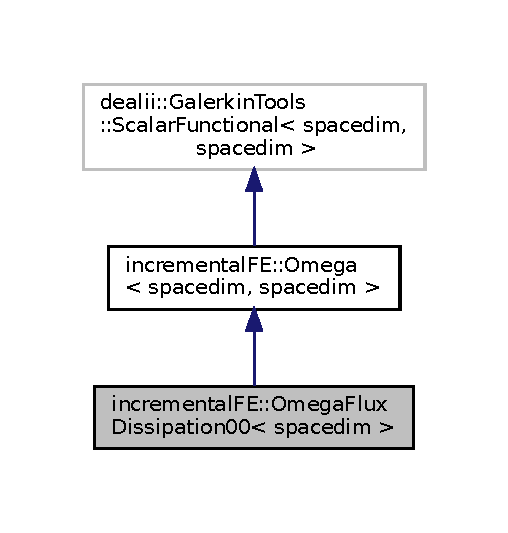
\includegraphics[width=244pt]{classincremental_f_e_1_1_omega_flux_dissipation00__inherit__graph}
\end{center}
\end{figure}


Collaboration diagram for incremental\+FE\+::Omega\+Flux\+Dissipation00$<$ spacedim $>$\+:\nopagebreak
\begin{figure}[H]
\begin{center}
\leavevmode
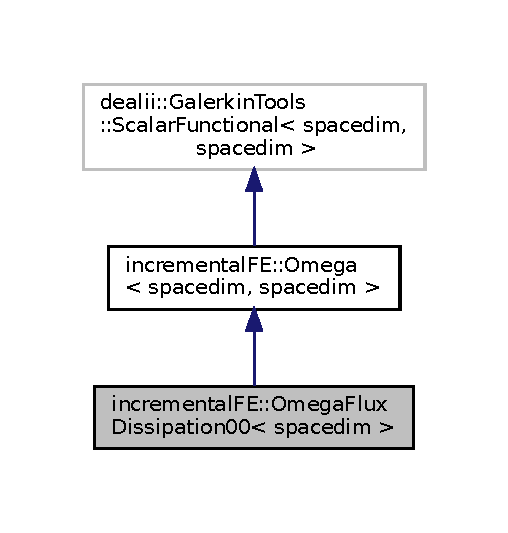
\includegraphics[width=244pt]{classincremental_f_e_1_1_omega_flux_dissipation00__coll__graph}
\end{center}
\end{figure}
\doxysubsection*{Public Member Functions}
\begin{DoxyCompactItemize}
\item 
\mbox{\hyperlink{classincremental_f_e_1_1_omega_flux_dissipation00_a37c7be7431a199da9fb1351fcdbe2c3f}{Omega\+Flux\+Dissipation00}} (const std\+::vector$<$ dealii\+::\+Galerkin\+Tools\+::\+Dependent\+Field$<$ spacedim, spacedim $>$$>$ e\+\_\+omega, const std\+::set$<$ \textbf{ dealii\+::types\+::material\+\_\+id} $>$ domain\+\_\+of\+\_\+integration, const dealii\+::\+Quadrature$<$ spacedim $>$ quadrature, \mbox{\hyperlink{classincremental_f_e_1_1_global_data_incremental_f_e}{Global\+Data\+Incremental\+FE}}$<$ spacedim $>$ \&\mbox{\hyperlink{classincremental_f_e_1_1_omega_3_01spacedim_00_01spacedim_01_4_afffe781a5a2032ec003032adc78e1bf3}{global\+\_\+data}}, const double \mbox{\hyperlink{classincremental_f_e_1_1_omega_flux_dissipation00_ac0bf17df1157750f539c2cb1a2aabcd4}{D}}, const unsigned int \mbox{\hyperlink{classincremental_f_e_1_1_omega_3_01spacedim_00_01spacedim_01_4_a6c95d57122261e8a2e26d3818251bc9b}{method}}, const double \mbox{\hyperlink{classincremental_f_e_1_1_omega_3_01spacedim_00_01spacedim_01_4_ad881c36804cc027c301f4f069756c2db}{alpha}}=0.\+0)
\item 
bool \mbox{\hyperlink{classincremental_f_e_1_1_omega_flux_dissipation00_ae1189d7eedba56295ee1e0acd2b9229f}{get\+\_\+values\+\_\+and\+\_\+derivatives}} (const \textbf{ dealii\+::\+Vector}$<$ double $>$ \&\textbf{ values}, const double, const dealii\+::\+Point$<$ spacedim $>$ \&, double \&omega, \textbf{ dealii\+::\+Vector}$<$ double $>$ \&d\+\_\+omega, dealii\+::\+Full\+Matrix$<$ double $>$ \&d2\+\_\+omega, const std\+::tuple$<$ bool, bool, bool $>$ requested\+\_\+quantities, const bool compute\+\_\+dq) const
\end{DoxyCompactItemize}
\doxysubsection*{Private Attributes}
\begin{DoxyCompactItemize}
\item 
const double \mbox{\hyperlink{classincremental_f_e_1_1_omega_flux_dissipation00_ac0bf17df1157750f539c2cb1a2aabcd4}{D}}
\end{DoxyCompactItemize}
\doxysubsection*{Additional Inherited Members}


\doxysubsection{Detailed Description}
\subsubsection*{template$<$unsigned int spacedim$>$\newline
class incremental\+F\+E\+::\+Omega\+Flux\+Dissipation00$<$ spacedim $>$}

Class defining a domain related scalar functional with the integrand

$ h^\Omega_\rho = \dfrac{1}{2 D c} \dot{\boldsymbol{I}} \cdot \dot{\boldsymbol{I}} $,

where $c$ is the species concentration and $\dot{\boldsymbol{I}}$ the corresponding flux.

The \char`\"{}mobility\char`\"{} $D$ is related to the usual \char`\"{}diffusion constant\char`\"{} $ \bar D $ by $D = \bar D/(RT)$. Moreover, it is related to the electrical mobility $\mu$ by $ D = \mu n/F$, where $n$ is the charge per molecule of the mobile species in multiples of the elementary charge and $F$ Faraday\textquotesingle{}s constant.

Ordering of quantities in \textbf{ Scalar\+Functional$<$spacedim, spacedim$>$\+::e\+\_\+omega} \+:~\newline
\mbox{[}0\mbox{]} $I_x$~\newline
 \mbox{[}1\mbox{]} $I_y$~\newline
 \mbox{[}2\mbox{]} $I_z$~\newline
 \mbox{[}3\mbox{]} $c$ 

\doxysubsection{Constructor \& Destructor Documentation}
\mbox{\Hypertarget{classincremental_f_e_1_1_omega_flux_dissipation00_a37c7be7431a199da9fb1351fcdbe2c3f}\label{classincremental_f_e_1_1_omega_flux_dissipation00_a37c7be7431a199da9fb1351fcdbe2c3f}} 
\index{incrementalFE::OmegaFluxDissipation00$<$ spacedim $>$@{incrementalFE::OmegaFluxDissipation00$<$ spacedim $>$}!OmegaFluxDissipation00@{OmegaFluxDissipation00}}
\index{OmegaFluxDissipation00@{OmegaFluxDissipation00}!incrementalFE::OmegaFluxDissipation00$<$ spacedim $>$@{incrementalFE::OmegaFluxDissipation00$<$ spacedim $>$}}
\doxysubsubsection{\texorpdfstring{OmegaFluxDissipation00()}{OmegaFluxDissipation00()}}
{\footnotesize\ttfamily template$<$unsigned int spacedim$>$ \\
\mbox{\hyperlink{classincremental_f_e_1_1_omega_flux_dissipation00}{incremental\+F\+E\+::\+Omega\+Flux\+Dissipation00}}$<$ spacedim $>$\+::\mbox{\hyperlink{classincremental_f_e_1_1_omega_flux_dissipation00}{Omega\+Flux\+Dissipation00}} (\begin{DoxyParamCaption}\item[{const std\+::vector$<$ dealii\+::\+Galerkin\+Tools\+::\+Dependent\+Field$<$ spacedim, spacedim $>$$>$}]{e\+\_\+omega,  }\item[{const std\+::set$<$ \textbf{ dealii\+::types\+::material\+\_\+id} $>$}]{domain\+\_\+of\+\_\+integration,  }\item[{const dealii\+::\+Quadrature$<$ spacedim $>$}]{quadrature,  }\item[{\mbox{\hyperlink{classincremental_f_e_1_1_global_data_incremental_f_e}{Global\+Data\+Incremental\+FE}}$<$ spacedim $>$ \&}]{global\+\_\+data,  }\item[{const double}]{D,  }\item[{const unsigned int}]{method,  }\item[{const double}]{alpha = {\ttfamily 0.0} }\end{DoxyParamCaption})\hspace{0.3cm}{\ttfamily [inline]}}

Constructor


\begin{DoxyParams}[1]{Parameters}
\mbox{\texttt{ in}}  & {\em e\+\_\+omega} & \textbf{ Scalar\+Functional$<$spacedim, spacedim$>$\+::e\+\_\+omega}\\
\hline
\mbox{\texttt{ in}}  & {\em domain\+\_\+of\+\_\+integration} & \textbf{ Scalar\+Functional$<$spacedim, spacedim$>$\+::domain\+\_\+of\+\_\+integration}\\
\hline
\mbox{\texttt{ in}}  & {\em quadrature} & \textbf{ Scalar\+Functional$<$spacedim, spacedim$>$\+::quadrature}\\
\hline
\mbox{\texttt{ in}}  & {\em global\+\_\+data} & \mbox{\hyperlink{classincremental_f_e_1_1_omega_3_01spacedim_00_01spacedim_01_4_afffe781a5a2032ec003032adc78e1bf3}{Omega$<$spacedim, spacedim$>$\+::global\+\_\+data}}\\
\hline
\mbox{\texttt{ in}}  & {\em D} & \mbox{\hyperlink{classincremental_f_e_1_1_omega_flux_dissipation00_ac0bf17df1157750f539c2cb1a2aabcd4}{Omega\+Flux\+Dissipation00\+::D}}\\
\hline
\mbox{\texttt{ in}}  & {\em method} & \mbox{\hyperlink{classincremental_f_e_1_1_omega_3_01spacedim_00_01spacedim_01_4_a6c95d57122261e8a2e26d3818251bc9b}{Omega$<$spacedim, spacedim$>$\+::method}}\\
\hline
\mbox{\texttt{ in}}  & {\em alpha} & \mbox{\hyperlink{classincremental_f_e_1_1_omega_3_01spacedim_00_01spacedim_01_4_ad881c36804cc027c301f4f069756c2db}{Omega$<$spacedim, spacedim$>$\+::alpha}} \\
\hline
\end{DoxyParams}


\doxysubsection{Member Function Documentation}
\mbox{\Hypertarget{classincremental_f_e_1_1_omega_flux_dissipation00_ae1189d7eedba56295ee1e0acd2b9229f}\label{classincremental_f_e_1_1_omega_flux_dissipation00_ae1189d7eedba56295ee1e0acd2b9229f}} 
\index{incrementalFE::OmegaFluxDissipation00$<$ spacedim $>$@{incrementalFE::OmegaFluxDissipation00$<$ spacedim $>$}!get\_values\_and\_derivatives@{get\_values\_and\_derivatives}}
\index{get\_values\_and\_derivatives@{get\_values\_and\_derivatives}!incrementalFE::OmegaFluxDissipation00$<$ spacedim $>$@{incrementalFE::OmegaFluxDissipation00$<$ spacedim $>$}}
\doxysubsubsection{\texorpdfstring{get\_values\_and\_derivatives()}{get\_values\_and\_derivatives()}}
{\footnotesize\ttfamily template$<$unsigned int spacedim$>$ \\
bool \mbox{\hyperlink{classincremental_f_e_1_1_omega_flux_dissipation00}{incremental\+F\+E\+::\+Omega\+Flux\+Dissipation00}}$<$ spacedim $>$\+::get\+\_\+values\+\_\+and\+\_\+derivatives (\begin{DoxyParamCaption}\item[{const \textbf{ dealii\+::\+Vector}$<$ double $>$ \&}]{values,  }\item[{const double}]{,  }\item[{const dealii\+::\+Point$<$ spacedim $>$ \&}]{,  }\item[{double \&}]{omega,  }\item[{\textbf{ dealii\+::\+Vector}$<$ double $>$ \&}]{d\+\_\+omega,  }\item[{dealii\+::\+Full\+Matrix$<$ double $>$ \&}]{d2\+\_\+omega,  }\item[{const std\+::tuple$<$ bool, bool, bool $>$}]{requested\+\_\+quantities,  }\item[{const bool}]{compute\+\_\+dq }\end{DoxyParamCaption}) const\hspace{0.3cm}{\ttfamily [inline]}, {\ttfamily [virtual]}}

\begin{DoxySeeAlso}{See also}
\mbox{\hyperlink{classincremental_f_e_1_1_omega_3_01spacedim_00_01spacedim_01_4_a40131354ef0a28ca48a0e6c9ed33aa33}{Omega$<$spacedim, spacedim$>$\+::get\+\_\+values\+\_\+and\+\_\+derivatives()}} 
\end{DoxySeeAlso}


Implements \mbox{\hyperlink{classincremental_f_e_1_1_omega_3_01spacedim_00_01spacedim_01_4_a40131354ef0a28ca48a0e6c9ed33aa33}{incremental\+F\+E\+::\+Omega$<$ spacedim, spacedim $>$}}.



\doxysubsection{Member Data Documentation}
\mbox{\Hypertarget{classincremental_f_e_1_1_omega_flux_dissipation00_ac0bf17df1157750f539c2cb1a2aabcd4}\label{classincremental_f_e_1_1_omega_flux_dissipation00_ac0bf17df1157750f539c2cb1a2aabcd4}} 
\index{incrementalFE::OmegaFluxDissipation00$<$ spacedim $>$@{incrementalFE::OmegaFluxDissipation00$<$ spacedim $>$}!D@{D}}
\index{D@{D}!incrementalFE::OmegaFluxDissipation00$<$ spacedim $>$@{incrementalFE::OmegaFluxDissipation00$<$ spacedim $>$}}
\doxysubsubsection{\texorpdfstring{D}{D}}
{\footnotesize\ttfamily template$<$unsigned int spacedim$>$ \\
const double \mbox{\hyperlink{classincremental_f_e_1_1_omega_flux_dissipation00}{incremental\+F\+E\+::\+Omega\+Flux\+Dissipation00}}$<$ spacedim $>$\+::D\hspace{0.3cm}{\ttfamily [private]}}

mobility 

The documentation for this class was generated from the following file\+:\begin{DoxyCompactItemize}
\item 
/home/sst/code/\+Incremental\+F\+E/\+Incremental\+F\+E/include/incremental\+\_\+fe/scalar\+\_\+functionals/\mbox{\hyperlink{omega__lib_8h}{omega\+\_\+lib.\+h}}\end{DoxyCompactItemize}

\hypertarget{classincremental_f_e_1_1_omega_flux_power00}{}\section{incremental\+FE\+:\+:Omega\+Flux\+Power00$<$ spacedim $>$ Class Template Reference}
\label{classincremental_f_e_1_1_omega_flux_power00}\index{incremental\+F\+E\+::\+Omega\+Flux\+Power00$<$ spacedim $>$@{incremental\+F\+E\+::\+Omega\+Flux\+Power00$<$ spacedim $>$}}


{\ttfamily \#include $<$omega\+\_\+lib.\+h$>$}



Inheritance diagram for incremental\+FE\+:\+:Omega\+Flux\+Power00$<$ spacedim $>$\+:\nopagebreak
\begin{figure}[H]
\begin{center}
\leavevmode
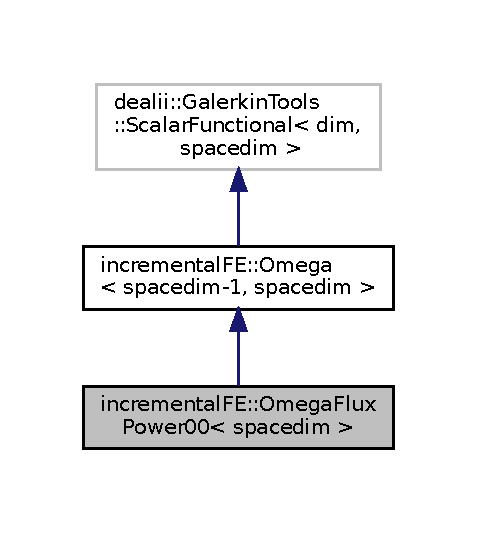
\includegraphics[width=216pt]{classincremental_f_e_1_1_omega_flux_power00__inherit__graph}
\end{center}
\end{figure}


Collaboration diagram for incremental\+FE\+:\+:Omega\+Flux\+Power00$<$ spacedim $>$\+:\nopagebreak
\begin{figure}[H]
\begin{center}
\leavevmode
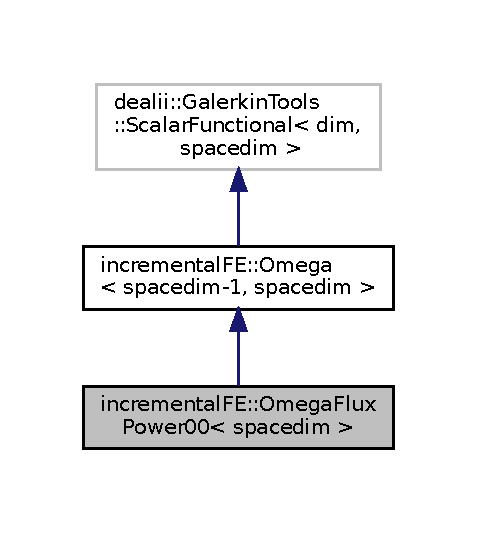
\includegraphics[width=216pt]{classincremental_f_e_1_1_omega_flux_power00__coll__graph}
\end{center}
\end{figure}
\subsection*{Public Member Functions}
\begin{DoxyCompactItemize}
\item 
\hyperlink{classincremental_f_e_1_1_omega_flux_power00_a90bd37bed7609d188bc543ecd466e198}{Omega\+Flux\+Power00} (const std\+::vector$<$ dealii\+::\+Galerkin\+Tools\+::\+Dependent\+Field$<$ spacedim-\/1, spacedim $>$$>$ e\+\_\+sigma, const std\+::set$<$ {\bf dealii\+::types\+::material\+\_\+id} $>$ domain\+\_\+of\+\_\+integration, const dealii\+::\+Quadrature$<$ spacedim-\/1 $>$ quadrature, \hyperlink{classincremental_f_e_1_1_global_data_incremental_f_e}{Global\+Data\+Incremental\+FE}$<$ spacedim $>$ \&\hyperlink{classincremental_f_e_1_1_omega_abd23d288a7a4a43f9b528be968cd2113}{global\+\_\+data}, dealii\+::\+Function$<$ spacedim $>$ \&\hyperlink{classincremental_f_e_1_1_omega_flux_power00_a9b8beb230f2a0609646ddebe08c1c236}{function\+\_\+mu}, const unsigned int \hyperlink{classincremental_f_e_1_1_omega_a7600d263ebf98129629e44fa67e8a58c}{method}, const double \hyperlink{classincremental_f_e_1_1_omega_a891688560ec0ad8dc5a0058a7b400269}{alpha}=0.\+0)
\item 
bool \hyperlink{classincremental_f_e_1_1_omega_flux_power00_abbcdc6c23167a34199401338b7fe058f}{get\+\_\+values\+\_\+and\+\_\+derivatives} (const {\bf dealii\+::\+Vector}$<$ double $>$ \&{\bf values}, const double t, const dealii\+::\+Point$<$ spacedim $>$ \&x, const dealii\+::\+Tensor$<$ 1, spacedim $>$ \&n, double \&sigma, {\bf dealii\+::\+Vector}$<$ double $>$ \&d\+\_\+sigma, dealii\+::\+Full\+Matrix$<$ double $>$ \&, const std\+::tuple$<$ bool, bool, bool $>$ requested\+\_\+quantities, const bool) const 
\end{DoxyCompactItemize}
\subsection*{Private Attributes}
\begin{DoxyCompactItemize}
\item 
dealii\+::\+Function$<$ spacedim $>$ \& \hyperlink{classincremental_f_e_1_1_omega_flux_power00_a9b8beb230f2a0609646ddebe08c1c236}{function\+\_\+mu}
\end{DoxyCompactItemize}
\subsection*{Additional Inherited Members}


\subsection{Detailed Description}
\subsubsection*{template$<$unsigned int spacedim$>$\\*
class incremental\+F\+E\+::\+Omega\+Flux\+Power00$<$ spacedim $>$}

Class defining an interface related scalar functional with the integrand

$ h^\Sigma_\tau = \bar\mu(t) \dot{\boldsymbol{I}} \cdot \boldsymbol{n} $

where $\bar\mu$ is a prescribed potential, and $\dot{\boldsymbol{I}}$ a flux.

Ordering of quantities in {\bf Scalar\+Functional\+::e\+\_\+sigma} \+:~\newline
\mbox{[}0\mbox{]} $I_x$~\newline
 \mbox{[}1\mbox{]} $I_y$~\newline
 \mbox{[}2\mbox{]} $I_z$~\newline
 

\subsection{Constructor \& Destructor Documentation}
\index{incremental\+F\+E\+::\+Omega\+Flux\+Power00@{incremental\+F\+E\+::\+Omega\+Flux\+Power00}!Omega\+Flux\+Power00@{Omega\+Flux\+Power00}}
\index{Omega\+Flux\+Power00@{Omega\+Flux\+Power00}!incremental\+F\+E\+::\+Omega\+Flux\+Power00@{incremental\+F\+E\+::\+Omega\+Flux\+Power00}}
\subsubsection[{\texorpdfstring{Omega\+Flux\+Power00(const std\+::vector$<$ dealii\+::\+Galerkin\+Tools\+::\+Dependent\+Field$<$ spacedim-\/1, spacedim $>$$>$ e\+\_\+sigma, const std\+::set$<$ dealii\+::types\+::material\+\_\+id $>$ domain\+\_\+of\+\_\+integration, const dealii\+::\+Quadrature$<$ spacedim-\/1 $>$ quadrature, Global\+Data\+Incremental\+F\+E$<$ spacedim $>$ \&global\+\_\+data, dealii\+::\+Function$<$ spacedim $>$ \&function\+\_\+mu, const unsigned int method, const double alpha=0.\+0)}{OmegaFluxPower00(const std::vector< dealii::GalerkinTools::DependentField< spacedim-1, spacedim >> e_sigma, const std::set< dealii::types::material_id > domain_of_integration, const dealii::Quadrature< spacedim-1 > quadrature, GlobalDataIncrementalFE< spacedim > &global_data, dealii::Function< spacedim > &function_mu, const unsigned int method, const double alpha=0.0)}}]{\setlength{\rightskip}{0pt plus 5cm}template$<$unsigned int spacedim$>$ {\bf incremental\+F\+E\+::\+Omega\+Flux\+Power00}$<$ spacedim $>$\+::{\bf Omega\+Flux\+Power00} (
\begin{DoxyParamCaption}
\item[{const std\+::vector$<$ dealii\+::\+Galerkin\+Tools\+::\+Dependent\+Field$<$ spacedim-\/1, spacedim $>$$>$}]{e\+\_\+sigma, }
\item[{const std\+::set$<$ {\bf dealii\+::types\+::material\+\_\+id} $>$}]{domain\+\_\+of\+\_\+integration, }
\item[{const dealii\+::\+Quadrature$<$ spacedim-\/1 $>$}]{quadrature, }
\item[{{\bf Global\+Data\+Incremental\+FE}$<$ spacedim $>$ \&}]{global\+\_\+data, }
\item[{dealii\+::\+Function$<$ spacedim $>$ \&}]{function\+\_\+mu, }
\item[{const unsigned int}]{method, }
\item[{const double}]{alpha = {\ttfamily 0.0}}
\end{DoxyParamCaption}
)\hspace{0.3cm}{\ttfamily [inline]}}\hypertarget{classincremental_f_e_1_1_omega_flux_power00_a90bd37bed7609d188bc543ecd466e198}{}\label{classincremental_f_e_1_1_omega_flux_power00_a90bd37bed7609d188bc543ecd466e198}
Constructor


\begin{DoxyParams}[1]{Parameters}
\mbox{\tt in}  & {\em e\+\_\+sigma} & {\bf Scalar\+Functional\+::e\+\_\+sigma}\\
\hline
\mbox{\tt in}  & {\em domain\+\_\+of\+\_\+integration} & {\bf Scalar\+Functional\+::domain\+\_\+of\+\_\+integration}\\
\hline
\mbox{\tt in}  & {\em quadrature} & {\bf Scalar\+Functional\+::quadrature}\\
\hline
\mbox{\tt in}  & {\em global\+\_\+data} & \hyperlink{classincremental_f_e_1_1_omega_abd23d288a7a4a43f9b528be968cd2113}{Omega\+::global\+\_\+data}\\
\hline
\mbox{\tt in}  & {\em function\+\_\+mu} & \hyperlink{classincremental_f_e_1_1_omega_flux_power00_a9b8beb230f2a0609646ddebe08c1c236}{Omega\+Flux\+Power00\+::function\+\_\+mu}\\
\hline
\mbox{\tt in}  & {\em method} & \hyperlink{classincremental_f_e_1_1_omega_a7600d263ebf98129629e44fa67e8a58c}{Omega\+::method}\\
\hline
\mbox{\tt in}  & {\em alpha} & \hyperlink{classincremental_f_e_1_1_omega_a891688560ec0ad8dc5a0058a7b400269}{Omega\+::alpha} \\
\hline
\end{DoxyParams}


\subsection{Member Function Documentation}
\index{incremental\+F\+E\+::\+Omega\+Flux\+Power00@{incremental\+F\+E\+::\+Omega\+Flux\+Power00}!get\+\_\+values\+\_\+and\+\_\+derivatives@{get\+\_\+values\+\_\+and\+\_\+derivatives}}
\index{get\+\_\+values\+\_\+and\+\_\+derivatives@{get\+\_\+values\+\_\+and\+\_\+derivatives}!incremental\+F\+E\+::\+Omega\+Flux\+Power00@{incremental\+F\+E\+::\+Omega\+Flux\+Power00}}
\subsubsection[{\texorpdfstring{get\+\_\+values\+\_\+and\+\_\+derivatives(const dealii\+::\+Vector$<$ double $>$ \&values, const double t, const dealii\+::\+Point$<$ spacedim $>$ \&x, const dealii\+::\+Tensor$<$ 1, spacedim $>$ \&n, double \&sigma, dealii\+::\+Vector$<$ double $>$ \&d\+\_\+sigma, dealii\+::\+Full\+Matrix$<$ double $>$ \&, const std\+::tuple$<$ bool, bool, bool $>$ requested\+\_\+quantities, const bool) const }{get_values_and_derivatives(const dealii::Vector< double > &values, const double t, const dealii::Point< spacedim > &x, const dealii::Tensor< 1, spacedim > &n, double &sigma, dealii::Vector< double > &d_sigma, dealii::FullMatrix< double > &, const std::tuple< bool, bool, bool > requested_quantities, const bool) const }}]{\setlength{\rightskip}{0pt plus 5cm}template$<$unsigned int spacedim$>$ bool {\bf incremental\+F\+E\+::\+Omega\+Flux\+Power00}$<$ spacedim $>$\+::get\+\_\+values\+\_\+and\+\_\+derivatives (
\begin{DoxyParamCaption}
\item[{const {\bf dealii\+::\+Vector}$<$ double $>$ \&}]{values, }
\item[{const double}]{t, }
\item[{const dealii\+::\+Point$<$ spacedim $>$ \&}]{x, }
\item[{const dealii\+::\+Tensor$<$ 1, spacedim $>$ \&}]{n, }
\item[{double \&}]{sigma, }
\item[{{\bf dealii\+::\+Vector}$<$ double $>$ \&}]{d\+\_\+sigma, }
\item[{dealii\+::\+Full\+Matrix$<$ double $>$ \&}]{, }
\item[{const std\+::tuple$<$ bool, bool, bool $>$}]{requested\+\_\+quantities, }
\item[{const bool}]{}
\end{DoxyParamCaption}
) const\hspace{0.3cm}{\ttfamily [inline]}, {\ttfamily [virtual]}}\hypertarget{classincremental_f_e_1_1_omega_flux_power00_abbcdc6c23167a34199401338b7fe058f}{}\label{classincremental_f_e_1_1_omega_flux_power00_abbcdc6c23167a34199401338b7fe058f}
\begin{DoxySeeAlso}{See also}
\hyperlink{classincremental_f_e_1_1_omega_a2f35d862aefa11151de5b7c7411e45df}{Omega\+::get\+\_\+values\+\_\+and\+\_\+derivatives()} 
\end{DoxySeeAlso}


Implements \hyperlink{classincremental_f_e_1_1_omega_a2f35d862aefa11151de5b7c7411e45df}{incremental\+F\+E\+::\+Omega$<$ spacedim-\/1, spacedim $>$}.



\subsection{Member Data Documentation}
\index{incremental\+F\+E\+::\+Omega\+Flux\+Power00@{incremental\+F\+E\+::\+Omega\+Flux\+Power00}!function\+\_\+mu@{function\+\_\+mu}}
\index{function\+\_\+mu@{function\+\_\+mu}!incremental\+F\+E\+::\+Omega\+Flux\+Power00@{incremental\+F\+E\+::\+Omega\+Flux\+Power00}}
\subsubsection[{\texorpdfstring{function\+\_\+mu}{function_mu}}]{\setlength{\rightskip}{0pt plus 5cm}template$<$unsigned int spacedim$>$ dealii\+::\+Function$<$spacedim$>$\& {\bf incremental\+F\+E\+::\+Omega\+Flux\+Power00}$<$ spacedim $>$\+::function\+\_\+mu\hspace{0.3cm}{\ttfamily [private]}}\hypertarget{classincremental_f_e_1_1_omega_flux_power00_a9b8beb230f2a0609646ddebe08c1c236}{}\label{classincremental_f_e_1_1_omega_flux_power00_a9b8beb230f2a0609646ddebe08c1c236}
Function determining $\bar \mu(t)$ 

The documentation for this class was generated from the following file\+:\begin{DoxyCompactItemize}
\item 
/home/sst/code/\+Incremental\+F\+E/\+Incremental\+F\+E/include/incremental\+\_\+fe/scalar\+\_\+functionals/\hyperlink{omega__lib_8h}{omega\+\_\+lib.\+h}\end{DoxyCompactItemize}

\hypertarget{classincremental_f_e_1_1_omega_interface_flux_dissipation00}{}\doxysection{incremental\+FE\+::Omega\+Interface\+Flux\+Dissipation00$<$ spacedim $>$ Class Template Reference}
\label{classincremental_f_e_1_1_omega_interface_flux_dissipation00}\index{incrementalFE::OmegaInterfaceFluxDissipation00$<$ spacedim $>$@{incrementalFE::OmegaInterfaceFluxDissipation00$<$ spacedim $>$}}


{\ttfamily \#include $<$omega\+\_\+lib.\+h$>$}



Inheritance diagram for incremental\+FE\+::Omega\+Interface\+Flux\+Dissipation00$<$ spacedim $>$\+:\nopagebreak
\begin{figure}[H]
\begin{center}
\leavevmode
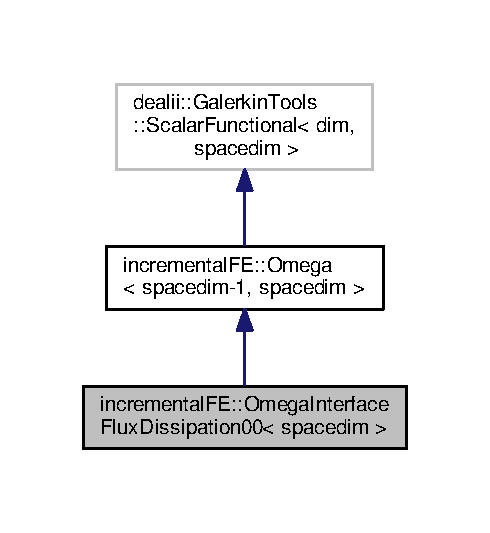
\includegraphics[width=254pt]{classincremental_f_e_1_1_omega_interface_flux_dissipation00__inherit__graph}
\end{center}
\end{figure}


Collaboration diagram for incremental\+FE\+::Omega\+Interface\+Flux\+Dissipation00$<$ spacedim $>$\+:\nopagebreak
\begin{figure}[H]
\begin{center}
\leavevmode
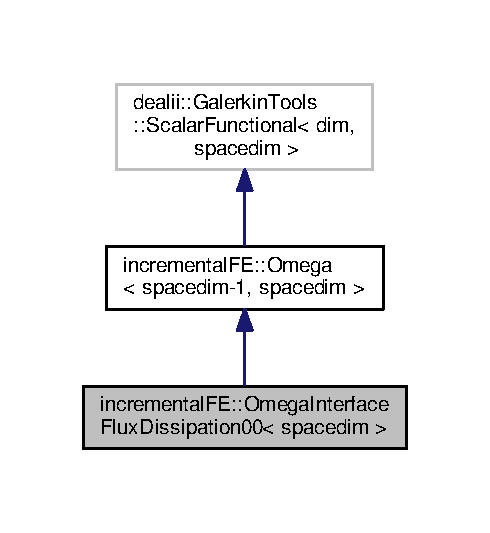
\includegraphics[width=254pt]{classincremental_f_e_1_1_omega_interface_flux_dissipation00__coll__graph}
\end{center}
\end{figure}
\doxysubsection*{Public Member Functions}
\begin{DoxyCompactItemize}
\item 
\mbox{\hyperlink{classincremental_f_e_1_1_omega_interface_flux_dissipation00_a57559567b075fc91c5d43d6d1da03b1e}{Omega\+Interface\+Flux\+Dissipation00}} (const std\+::vector$<$ dealii\+::\+Galerkin\+Tools\+::\+Dependent\+Field$<$ spacedim-\/1, spacedim $>$$>$ e\+\_\+sigma, const std\+::set$<$ \textbf{ dealii\+::types\+::material\+\_\+id} $>$ domain\+\_\+of\+\_\+integration, const dealii\+::\+Quadrature$<$ spacedim-\/1 $>$ quadrature, \mbox{\hyperlink{classincremental_f_e_1_1_global_data_incremental_f_e}{Global\+Data\+Incremental\+FE}}$<$ spacedim $>$ \&\mbox{\hyperlink{classincremental_f_e_1_1_omega_abd23d288a7a4a43f9b528be968cd2113}{global\+\_\+data}}, const double \mbox{\hyperlink{classincremental_f_e_1_1_omega_interface_flux_dissipation00_ab6efbe2a1c165f99e02c22e4df530d0b}{D}}, const unsigned int \mbox{\hyperlink{classincremental_f_e_1_1_omega_a7600d263ebf98129629e44fa67e8a58c}{method}}, const double \mbox{\hyperlink{classincremental_f_e_1_1_omega_ae09e949c58fe8e7a7f3ae6031e6435b9}{alpha}}=0.\+0)
\item 
bool \mbox{\hyperlink{classincremental_f_e_1_1_omega_interface_flux_dissipation00_ac0fd530029ec25b4684f1c2e644362b8}{get\+\_\+values\+\_\+and\+\_\+derivatives}} (const \textbf{ dealii\+::\+Vector}$<$ double $>$ \&\textbf{ values}, const double, const dealii\+::\+Point$<$ spacedim $>$ \&, const dealii\+::\+Tensor$<$ 1, spacedim $>$ \&n, double \&sigma, \textbf{ dealii\+::\+Vector}$<$ double $>$ \&d\+\_\+sigma, dealii\+::\+Full\+Matrix$<$ double $>$ \&d2\+\_\+sigma, const std\+::tuple$<$ bool, bool, bool $>$ requested\+\_\+quantities, const bool) const
\end{DoxyCompactItemize}
\doxysubsection*{Private Attributes}
\begin{DoxyCompactItemize}
\item 
const double \mbox{\hyperlink{classincremental_f_e_1_1_omega_interface_flux_dissipation00_ab6efbe2a1c165f99e02c22e4df530d0b}{D}}
\end{DoxyCompactItemize}
\doxysubsection*{Additional Inherited Members}


\doxysubsection{Detailed Description}
\subsubsection*{template$<$unsigned int spacedim$>$\newline
class incremental\+F\+E\+::\+Omega\+Interface\+Flux\+Dissipation00$<$ spacedim $>$}

Class defining an interface related scalar functional with the integrand

$ \omega^\Sigma = 1/(2D) \left(\dot{\boldsymbol{I}} \cdot \boldsymbol{n}\right)^2 $

where $D$ is a dissipation constant, and $\dot{\boldsymbol{I}}$ a flux.

Ordering of quantities in \textbf{ Scalar\+Functional\+::e\+\_\+sigma} \+:~\newline
\mbox{[}0\mbox{]} $I_x$~\newline
 \mbox{[}1\mbox{]} $I_y$~\newline
 \mbox{[}2\mbox{]} $I_z$~\newline
 

\doxysubsection{Constructor \& Destructor Documentation}
\mbox{\Hypertarget{classincremental_f_e_1_1_omega_interface_flux_dissipation00_a57559567b075fc91c5d43d6d1da03b1e}\label{classincremental_f_e_1_1_omega_interface_flux_dissipation00_a57559567b075fc91c5d43d6d1da03b1e}} 
\index{incrementalFE::OmegaInterfaceFluxDissipation00$<$ spacedim $>$@{incrementalFE::OmegaInterfaceFluxDissipation00$<$ spacedim $>$}!OmegaInterfaceFluxDissipation00@{OmegaInterfaceFluxDissipation00}}
\index{OmegaInterfaceFluxDissipation00@{OmegaInterfaceFluxDissipation00}!incrementalFE::OmegaInterfaceFluxDissipation00$<$ spacedim $>$@{incrementalFE::OmegaInterfaceFluxDissipation00$<$ spacedim $>$}}
\doxysubsubsection{\texorpdfstring{OmegaInterfaceFluxDissipation00()}{OmegaInterfaceFluxDissipation00()}}
{\footnotesize\ttfamily template$<$unsigned int spacedim$>$ \\
\mbox{\hyperlink{classincremental_f_e_1_1_omega_interface_flux_dissipation00}{incremental\+F\+E\+::\+Omega\+Interface\+Flux\+Dissipation00}}$<$ spacedim $>$\+::\mbox{\hyperlink{classincremental_f_e_1_1_omega_interface_flux_dissipation00}{Omega\+Interface\+Flux\+Dissipation00}} (\begin{DoxyParamCaption}\item[{const std\+::vector$<$ dealii\+::\+Galerkin\+Tools\+::\+Dependent\+Field$<$ spacedim-\/1, spacedim $>$$>$}]{e\+\_\+sigma,  }\item[{const std\+::set$<$ \textbf{ dealii\+::types\+::material\+\_\+id} $>$}]{domain\+\_\+of\+\_\+integration,  }\item[{const dealii\+::\+Quadrature$<$ spacedim-\/1 $>$}]{quadrature,  }\item[{\mbox{\hyperlink{classincremental_f_e_1_1_global_data_incremental_f_e}{Global\+Data\+Incremental\+FE}}$<$ spacedim $>$ \&}]{global\+\_\+data,  }\item[{const double}]{D,  }\item[{const unsigned int}]{method,  }\item[{const double}]{alpha = {\ttfamily 0.0} }\end{DoxyParamCaption})\hspace{0.3cm}{\ttfamily [inline]}}

Constructor


\begin{DoxyParams}[1]{Parameters}
\mbox{\texttt{ in}}  & {\em e\+\_\+sigma} & \textbf{ Scalar\+Functional\+::e\+\_\+sigma}\\
\hline
\mbox{\texttt{ in}}  & {\em domain\+\_\+of\+\_\+integration} & \textbf{ Scalar\+Functional\+::domain\+\_\+of\+\_\+integration}\\
\hline
\mbox{\texttt{ in}}  & {\em quadrature} & \textbf{ Scalar\+Functional\+::quadrature}\\
\hline
\mbox{\texttt{ in}}  & {\em global\+\_\+data} & \mbox{\hyperlink{classincremental_f_e_1_1_omega_abd23d288a7a4a43f9b528be968cd2113}{Omega\+::global\+\_\+data}}\\
\hline
\mbox{\texttt{ in}}  & {\em D} & \mbox{\hyperlink{classincremental_f_e_1_1_omega_interface_flux_dissipation00_ab6efbe2a1c165f99e02c22e4df530d0b}{Omega\+Interface\+Flux\+Dissipation00\+::D}}\\
\hline
\mbox{\texttt{ in}}  & {\em method} & \mbox{\hyperlink{classincremental_f_e_1_1_omega_a7600d263ebf98129629e44fa67e8a58c}{Omega\+::method}}\\
\hline
\mbox{\texttt{ in}}  & {\em alpha} & \mbox{\hyperlink{classincremental_f_e_1_1_omega_ae09e949c58fe8e7a7f3ae6031e6435b9}{Omega\+::alpha}} \\
\hline
\end{DoxyParams}


\doxysubsection{Member Function Documentation}
\mbox{\Hypertarget{classincremental_f_e_1_1_omega_interface_flux_dissipation00_ac0fd530029ec25b4684f1c2e644362b8}\label{classincremental_f_e_1_1_omega_interface_flux_dissipation00_ac0fd530029ec25b4684f1c2e644362b8}} 
\index{incrementalFE::OmegaInterfaceFluxDissipation00$<$ spacedim $>$@{incrementalFE::OmegaInterfaceFluxDissipation00$<$ spacedim $>$}!get\_values\_and\_derivatives@{get\_values\_and\_derivatives}}
\index{get\_values\_and\_derivatives@{get\_values\_and\_derivatives}!incrementalFE::OmegaInterfaceFluxDissipation00$<$ spacedim $>$@{incrementalFE::OmegaInterfaceFluxDissipation00$<$ spacedim $>$}}
\doxysubsubsection{\texorpdfstring{get\_values\_and\_derivatives()}{get\_values\_and\_derivatives()}}
{\footnotesize\ttfamily template$<$unsigned int spacedim$>$ \\
bool \mbox{\hyperlink{classincremental_f_e_1_1_omega_interface_flux_dissipation00}{incremental\+F\+E\+::\+Omega\+Interface\+Flux\+Dissipation00}}$<$ spacedim $>$\+::get\+\_\+values\+\_\+and\+\_\+derivatives (\begin{DoxyParamCaption}\item[{const \textbf{ dealii\+::\+Vector}$<$ double $>$ \&}]{values,  }\item[{const double}]{,  }\item[{const dealii\+::\+Point$<$ spacedim $>$ \&}]{,  }\item[{const dealii\+::\+Tensor$<$ 1, spacedim $>$ \&}]{n,  }\item[{double \&}]{sigma,  }\item[{\textbf{ dealii\+::\+Vector}$<$ double $>$ \&}]{d\+\_\+sigma,  }\item[{dealii\+::\+Full\+Matrix$<$ double $>$ \&}]{d2\+\_\+sigma,  }\item[{const std\+::tuple$<$ bool, bool, bool $>$}]{requested\+\_\+quantities,  }\item[{const bool}]{ }\end{DoxyParamCaption}) const\hspace{0.3cm}{\ttfamily [inline]}, {\ttfamily [virtual]}}

\begin{DoxySeeAlso}{See also}
\mbox{\hyperlink{classincremental_f_e_1_1_omega_a2f35d862aefa11151de5b7c7411e45df}{Omega\+::get\+\_\+values\+\_\+and\+\_\+derivatives()}} 
\end{DoxySeeAlso}


Implements \mbox{\hyperlink{classincremental_f_e_1_1_omega_a2f35d862aefa11151de5b7c7411e45df}{incremental\+F\+E\+::\+Omega$<$ spacedim-\/1, spacedim $>$}}.



\doxysubsection{Member Data Documentation}
\mbox{\Hypertarget{classincremental_f_e_1_1_omega_interface_flux_dissipation00_ab6efbe2a1c165f99e02c22e4df530d0b}\label{classincremental_f_e_1_1_omega_interface_flux_dissipation00_ab6efbe2a1c165f99e02c22e4df530d0b}} 
\index{incrementalFE::OmegaInterfaceFluxDissipation00$<$ spacedim $>$@{incrementalFE::OmegaInterfaceFluxDissipation00$<$ spacedim $>$}!D@{D}}
\index{D@{D}!incrementalFE::OmegaInterfaceFluxDissipation00$<$ spacedim $>$@{incrementalFE::OmegaInterfaceFluxDissipation00$<$ spacedim $>$}}
\doxysubsubsection{\texorpdfstring{D}{D}}
{\footnotesize\ttfamily template$<$unsigned int spacedim$>$ \\
const double \mbox{\hyperlink{classincremental_f_e_1_1_omega_interface_flux_dissipation00}{incremental\+F\+E\+::\+Omega\+Interface\+Flux\+Dissipation00}}$<$ spacedim $>$\+::D\hspace{0.3cm}{\ttfamily [private]}}

constant $D$ 

The documentation for this class was generated from the following file\+:\begin{DoxyCompactItemize}
\item 
/home/sst/code/\+Incremental\+F\+E/\+Incremental\+F\+E/include/incremental\+\_\+fe/scalar\+\_\+functionals/\mbox{\hyperlink{omega__lib_8h}{omega\+\_\+lib.\+h}}\end{DoxyCompactItemize}

\hypertarget{classincremental_f_e_1_1_omega_mixed_term00}{}\section{incremental\+FE\+:\+:Omega\+Mixed\+Term00$<$ spacedim $>$ Class Template Reference}
\label{classincremental_f_e_1_1_omega_mixed_term00}\index{incremental\+F\+E\+::\+Omega\+Mixed\+Term00$<$ spacedim $>$@{incremental\+F\+E\+::\+Omega\+Mixed\+Term00$<$ spacedim $>$}}


{\ttfamily \#include $<$omega\+\_\+lib.\+h$>$}



Inheritance diagram for incremental\+FE\+:\+:Omega\+Mixed\+Term00$<$ spacedim $>$\+:\nopagebreak
\begin{figure}[H]
\begin{center}
\leavevmode
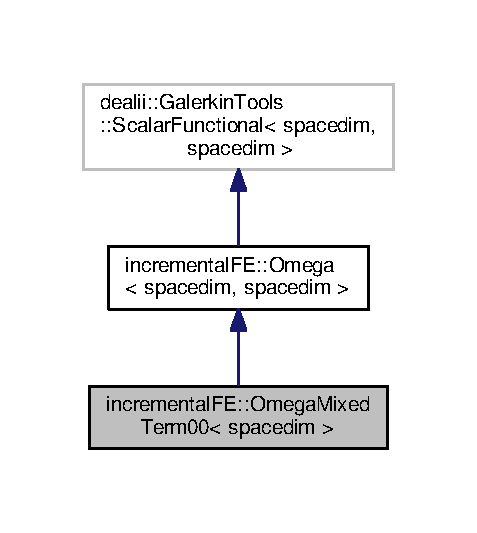
\includegraphics[width=229pt]{classincremental_f_e_1_1_omega_mixed_term00__inherit__graph}
\end{center}
\end{figure}


Collaboration diagram for incremental\+FE\+:\+:Omega\+Mixed\+Term00$<$ spacedim $>$\+:\nopagebreak
\begin{figure}[H]
\begin{center}
\leavevmode
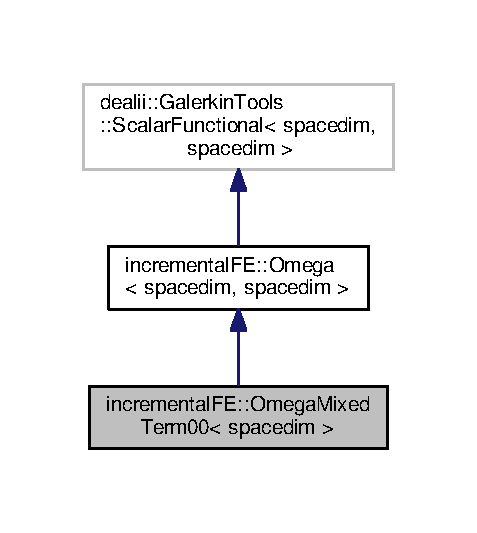
\includegraphics[width=229pt]{classincremental_f_e_1_1_omega_mixed_term00__coll__graph}
\end{center}
\end{figure}
\subsection*{Public Member Functions}
\begin{DoxyCompactItemize}
\item 
\hyperlink{classincremental_f_e_1_1_omega_mixed_term00_afe85ad649df64684d32abdc74bc2f5d6}{Omega\+Mixed\+Term00} (const std\+::vector$<$ dealii\+::\+Galerkin\+Tools\+::\+Dependent\+Field$<$ spacedim, spacedim $>$$>$ e\+\_\+omega, const std\+::set$<$ {\bf dealii\+::types\+::material\+\_\+id} $>$ domain\+\_\+of\+\_\+integration, const dealii\+::\+Quadrature$<$ spacedim $>$ quadrature, \hyperlink{classincremental_f_e_1_1_global_data_incremental_f_e}{Global\+Data\+Incremental\+FE}$<$ spacedim $>$ \&\hyperlink{classincremental_f_e_1_1_omega_3_01spacedim_00_01spacedim_01_4_afffe781a5a2032ec003032adc78e1bf3}{global\+\_\+data}, const unsigned int \hyperlink{classincremental_f_e_1_1_omega_3_01spacedim_00_01spacedim_01_4_a6c95d57122261e8a2e26d3818251bc9b}{method}, const double \hyperlink{classincremental_f_e_1_1_omega_3_01spacedim_00_01spacedim_01_4_ad881c36804cc027c301f4f069756c2db}{alpha}=0.\+0)
\item 
bool \hyperlink{classincremental_f_e_1_1_omega_mixed_term00_abf975855eb0155318ad152e7fbac11d1}{get\+\_\+values\+\_\+and\+\_\+derivatives} (const {\bf dealii\+::\+Vector}$<$ double $>$ \&{\bf values}, const double, const dealii\+::\+Point$<$ spacedim $>$ \&, double \&omega, {\bf dealii\+::\+Vector}$<$ double $>$ \&d\+\_\+omega, dealii\+::\+Full\+Matrix$<$ double $>$ \&d2\+\_\+omega, const std\+::tuple$<$ bool, bool, bool $>$ requested\+\_\+quantities, const bool) const 
\end{DoxyCompactItemize}
\subsection*{Additional Inherited Members}


\subsection{Detailed Description}
\subsubsection*{template$<$unsigned int spacedim$>$\\*
class incremental\+F\+E\+::\+Omega\+Mixed\+Term00$<$ spacedim $>$}

Class defining a domain related scalar functional with the integrand

$ h^\Omega_\rho = -\dot{c}\eta $,

where $c$ is a species concentration and $\eta$ the corresponding potential.

Ordering of quantities in {\bf Scalar\+Functional$<$spacedim, spacedim$>$\+::e\+\_\+omega} \+:~\newline
\mbox{[}0\mbox{]} $c$~\newline
 \mbox{[}1\mbox{]} $\eta$ 

\subsection{Constructor \& Destructor Documentation}
\index{incremental\+F\+E\+::\+Omega\+Mixed\+Term00@{incremental\+F\+E\+::\+Omega\+Mixed\+Term00}!Omega\+Mixed\+Term00@{Omega\+Mixed\+Term00}}
\index{Omega\+Mixed\+Term00@{Omega\+Mixed\+Term00}!incremental\+F\+E\+::\+Omega\+Mixed\+Term00@{incremental\+F\+E\+::\+Omega\+Mixed\+Term00}}
\subsubsection[{\texorpdfstring{Omega\+Mixed\+Term00(const std\+::vector$<$ dealii\+::\+Galerkin\+Tools\+::\+Dependent\+Field$<$ spacedim, spacedim $>$$>$ e\+\_\+omega, const std\+::set$<$ dealii\+::types\+::material\+\_\+id $>$ domain\+\_\+of\+\_\+integration, const dealii\+::\+Quadrature$<$ spacedim $>$ quadrature, Global\+Data\+Incremental\+F\+E$<$ spacedim $>$ \&global\+\_\+data, const unsigned int method, const double alpha=0.\+0)}{OmegaMixedTerm00(const std::vector< dealii::GalerkinTools::DependentField< spacedim, spacedim >> e_omega, const std::set< dealii::types::material_id > domain_of_integration, const dealii::Quadrature< spacedim > quadrature, GlobalDataIncrementalFE< spacedim > &global_data, const unsigned int method, const double alpha=0.0)}}]{\setlength{\rightskip}{0pt plus 5cm}template$<$unsigned int spacedim$>$ {\bf incremental\+F\+E\+::\+Omega\+Mixed\+Term00}$<$ spacedim $>$\+::{\bf Omega\+Mixed\+Term00} (
\begin{DoxyParamCaption}
\item[{const std\+::vector$<$ dealii\+::\+Galerkin\+Tools\+::\+Dependent\+Field$<$ spacedim, spacedim $>$$>$}]{e\+\_\+omega, }
\item[{const std\+::set$<$ {\bf dealii\+::types\+::material\+\_\+id} $>$}]{domain\+\_\+of\+\_\+integration, }
\item[{const dealii\+::\+Quadrature$<$ spacedim $>$}]{quadrature, }
\item[{{\bf Global\+Data\+Incremental\+FE}$<$ spacedim $>$ \&}]{global\+\_\+data, }
\item[{const unsigned int}]{method, }
\item[{const double}]{alpha = {\ttfamily 0.0}}
\end{DoxyParamCaption}
)\hspace{0.3cm}{\ttfamily [inline]}}\hypertarget{classincremental_f_e_1_1_omega_mixed_term00_afe85ad649df64684d32abdc74bc2f5d6}{}\label{classincremental_f_e_1_1_omega_mixed_term00_afe85ad649df64684d32abdc74bc2f5d6}
Constructor


\begin{DoxyParams}[1]{Parameters}
\mbox{\tt in}  & {\em e\+\_\+omega} & {\bf Scalar\+Functional$<$spacedim, spacedim$>$\+::e\+\_\+omega}\\
\hline
\mbox{\tt in}  & {\em domain\+\_\+of\+\_\+integration} & {\bf Scalar\+Functional$<$spacedim, spacedim$>$\+::domain\+\_\+of\+\_\+integration}\\
\hline
\mbox{\tt in}  & {\em quadrature} & {\bf Scalar\+Functional$<$spacedim, spacedim$>$\+::quadrature}\\
\hline
\mbox{\tt in}  & {\em global\+\_\+data} & \hyperlink{classincremental_f_e_1_1_omega_3_01spacedim_00_01spacedim_01_4_afffe781a5a2032ec003032adc78e1bf3}{Omega$<$spacedim, spacedim$>$\+::global\+\_\+data}\\
\hline
\mbox{\tt in}  & {\em method} & \hyperlink{classincremental_f_e_1_1_omega_3_01spacedim_00_01spacedim_01_4_a6c95d57122261e8a2e26d3818251bc9b}{Omega$<$spacedim, spacedim$>$\+::method}\\
\hline
\mbox{\tt in}  & {\em alpha} & \hyperlink{classincremental_f_e_1_1_omega_3_01spacedim_00_01spacedim_01_4_ad881c36804cc027c301f4f069756c2db}{Omega$<$spacedim, spacedim$>$\+::alpha} \\
\hline
\end{DoxyParams}


\subsection{Member Function Documentation}
\index{incremental\+F\+E\+::\+Omega\+Mixed\+Term00@{incremental\+F\+E\+::\+Omega\+Mixed\+Term00}!get\+\_\+values\+\_\+and\+\_\+derivatives@{get\+\_\+values\+\_\+and\+\_\+derivatives}}
\index{get\+\_\+values\+\_\+and\+\_\+derivatives@{get\+\_\+values\+\_\+and\+\_\+derivatives}!incremental\+F\+E\+::\+Omega\+Mixed\+Term00@{incremental\+F\+E\+::\+Omega\+Mixed\+Term00}}
\subsubsection[{\texorpdfstring{get\+\_\+values\+\_\+and\+\_\+derivatives(const dealii\+::\+Vector$<$ double $>$ \&values, const double, const dealii\+::\+Point$<$ spacedim $>$ \&, double \&omega, dealii\+::\+Vector$<$ double $>$ \&d\+\_\+omega, dealii\+::\+Full\+Matrix$<$ double $>$ \&d2\+\_\+omega, const std\+::tuple$<$ bool, bool, bool $>$ requested\+\_\+quantities, const bool) const }{get_values_and_derivatives(const dealii::Vector< double > &values, const double, const dealii::Point< spacedim > &, double &omega, dealii::Vector< double > &d_omega, dealii::FullMatrix< double > &d2_omega, const std::tuple< bool, bool, bool > requested_quantities, const bool) const }}]{\setlength{\rightskip}{0pt plus 5cm}template$<$unsigned int spacedim$>$ bool {\bf incremental\+F\+E\+::\+Omega\+Mixed\+Term00}$<$ spacedim $>$\+::get\+\_\+values\+\_\+and\+\_\+derivatives (
\begin{DoxyParamCaption}
\item[{const {\bf dealii\+::\+Vector}$<$ double $>$ \&}]{values, }
\item[{const double}]{, }
\item[{const dealii\+::\+Point$<$ spacedim $>$ \&}]{, }
\item[{double \&}]{omega, }
\item[{{\bf dealii\+::\+Vector}$<$ double $>$ \&}]{d\+\_\+omega, }
\item[{dealii\+::\+Full\+Matrix$<$ double $>$ \&}]{d2\+\_\+omega, }
\item[{const std\+::tuple$<$ bool, bool, bool $>$}]{requested\+\_\+quantities, }
\item[{const bool}]{}
\end{DoxyParamCaption}
) const\hspace{0.3cm}{\ttfamily [inline]}, {\ttfamily [virtual]}}\hypertarget{classincremental_f_e_1_1_omega_mixed_term00_abf975855eb0155318ad152e7fbac11d1}{}\label{classincremental_f_e_1_1_omega_mixed_term00_abf975855eb0155318ad152e7fbac11d1}
\begin{DoxySeeAlso}{See also}
\hyperlink{classincremental_f_e_1_1_omega_3_01spacedim_00_01spacedim_01_4_a40131354ef0a28ca48a0e6c9ed33aa33}{Omega$<$spacedim, spacedim$>$\+::get\+\_\+values\+\_\+and\+\_\+derivatives()} 
\end{DoxySeeAlso}


Implements \hyperlink{classincremental_f_e_1_1_omega_3_01spacedim_00_01spacedim_01_4_a40131354ef0a28ca48a0e6c9ed33aa33}{incremental\+F\+E\+::\+Omega$<$ spacedim, spacedim $>$}.



The documentation for this class was generated from the following file\+:\begin{DoxyCompactItemize}
\item 
/home/sst/code/\+Incremental\+F\+E/\+Incremental\+F\+E/include/incremental\+\_\+fe/scalar\+\_\+functionals/\hyperlink{omega__lib_8h}{omega\+\_\+lib.\+h}\end{DoxyCompactItemize}

\hypertarget{classincremental_f_e_1_1_omega_mixed_term01}{}\section{incremental\+FE\+:\+:Omega\+Mixed\+Term01$<$ spacedim $>$ Class Template Reference}
\label{classincremental_f_e_1_1_omega_mixed_term01}\index{incremental\+F\+E\+::\+Omega\+Mixed\+Term01$<$ spacedim $>$@{incremental\+F\+E\+::\+Omega\+Mixed\+Term01$<$ spacedim $>$}}


{\ttfamily \#include $<$omega\+\_\+lib.\+h$>$}



Inheritance diagram for incremental\+FE\+:\+:Omega\+Mixed\+Term01$<$ spacedim $>$\+:\nopagebreak
\begin{figure}[H]
\begin{center}
\leavevmode
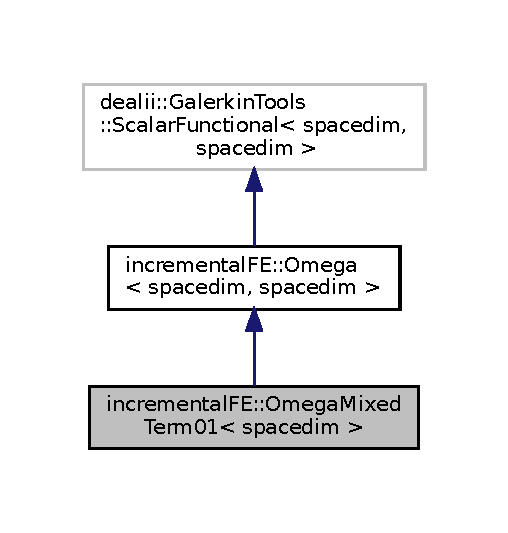
\includegraphics[width=229pt]{classincremental_f_e_1_1_omega_mixed_term01__inherit__graph}
\end{center}
\end{figure}


Collaboration diagram for incremental\+FE\+:\+:Omega\+Mixed\+Term01$<$ spacedim $>$\+:\nopagebreak
\begin{figure}[H]
\begin{center}
\leavevmode
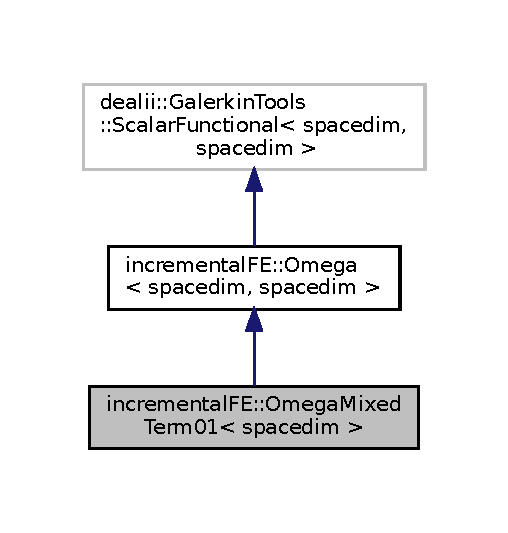
\includegraphics[width=229pt]{classincremental_f_e_1_1_omega_mixed_term01__coll__graph}
\end{center}
\end{figure}
\subsection*{Public Member Functions}
\begin{DoxyCompactItemize}
\item 
\hyperlink{classincremental_f_e_1_1_omega_mixed_term01_a45dcc5a37906872c6ab5a5090f87d206}{Omega\+Mixed\+Term01} (const std\+::vector$<$ dealii\+::\+Galerkin\+Tools\+::\+Dependent\+Field$<$ spacedim, spacedim $>$$>$ e\+\_\+omega, const std\+::set$<$ {\bf dealii\+::types\+::material\+\_\+id} $>$ domain\+\_\+of\+\_\+integration, const dealii\+::\+Quadrature$<$ spacedim $>$ quadrature, \hyperlink{classincremental_f_e_1_1_global_data_incremental_f_e}{Global\+Data\+Incremental\+FE}$<$ spacedim $>$ \&\hyperlink{classincremental_f_e_1_1_omega_3_01spacedim_00_01spacedim_01_4_afffe781a5a2032ec003032adc78e1bf3}{global\+\_\+data}, const unsigned int \hyperlink{classincremental_f_e_1_1_omega_3_01spacedim_00_01spacedim_01_4_a6c95d57122261e8a2e26d3818251bc9b}{method}, const double \hyperlink{classincremental_f_e_1_1_omega_3_01spacedim_00_01spacedim_01_4_ad881c36804cc027c301f4f069756c2db}{alpha}=0.\+0)
\item 
bool \hyperlink{classincremental_f_e_1_1_omega_mixed_term01_a6fe47df6c774ba07cb3455616997dfe7}{get\+\_\+values\+\_\+and\+\_\+derivatives} (const {\bf dealii\+::\+Vector}$<$ double $>$ \&{\bf values}, const double, const dealii\+::\+Point$<$ spacedim $>$ \&, double \&omega, {\bf dealii\+::\+Vector}$<$ double $>$ \&d\+\_\+omega, dealii\+::\+Full\+Matrix$<$ double $>$ \&d2\+\_\+omega, const std\+::tuple$<$ bool, bool, bool $>$ requested\+\_\+quantities, const bool) const 
\end{DoxyCompactItemize}
\subsection*{Additional Inherited Members}


\subsection{Detailed Description}
\subsubsection*{template$<$unsigned int spacedim$>$\\*
class incremental\+F\+E\+::\+Omega\+Mixed\+Term01$<$ spacedim $>$}

Class defining a domain related scalar functional with the integrand

$ h^\Omega_\rho = -\dot{\boldsymbol{D}} \cdot \boldsymbol{E} $,

where $\boldsymbol{D}$ and $\boldsymbol{E}$ are conjugate fields.

Ordering of quantities in {\bf Scalar\+Functional$<$spacedim, spacedim$>$\+::e\+\_\+omega} \+:~\newline
\mbox{[}0\mbox{]} $D_x$~\newline
 \mbox{[}1\mbox{]} $D_y$~\newline
 \mbox{[}2\mbox{]} $D_z$~\newline
 \mbox{[}3\mbox{]} $E_x$~\newline
 \mbox{[}4\mbox{]} $E_y$~\newline
 \mbox{[}5\mbox{]} $E_z$~\newline
 

\subsection{Constructor \& Destructor Documentation}
\index{incremental\+F\+E\+::\+Omega\+Mixed\+Term01@{incremental\+F\+E\+::\+Omega\+Mixed\+Term01}!Omega\+Mixed\+Term01@{Omega\+Mixed\+Term01}}
\index{Omega\+Mixed\+Term01@{Omega\+Mixed\+Term01}!incremental\+F\+E\+::\+Omega\+Mixed\+Term01@{incremental\+F\+E\+::\+Omega\+Mixed\+Term01}}
\subsubsection[{\texorpdfstring{Omega\+Mixed\+Term01(const std\+::vector$<$ dealii\+::\+Galerkin\+Tools\+::\+Dependent\+Field$<$ spacedim, spacedim $>$$>$ e\+\_\+omega, const std\+::set$<$ dealii\+::types\+::material\+\_\+id $>$ domain\+\_\+of\+\_\+integration, const dealii\+::\+Quadrature$<$ spacedim $>$ quadrature, Global\+Data\+Incremental\+F\+E$<$ spacedim $>$ \&global\+\_\+data, const unsigned int method, const double alpha=0.\+0)}{OmegaMixedTerm01(const std::vector< dealii::GalerkinTools::DependentField< spacedim, spacedim >> e_omega, const std::set< dealii::types::material_id > domain_of_integration, const dealii::Quadrature< spacedim > quadrature, GlobalDataIncrementalFE< spacedim > &global_data, const unsigned int method, const double alpha=0.0)}}]{\setlength{\rightskip}{0pt plus 5cm}template$<$unsigned int spacedim$>$ {\bf incremental\+F\+E\+::\+Omega\+Mixed\+Term01}$<$ spacedim $>$\+::{\bf Omega\+Mixed\+Term01} (
\begin{DoxyParamCaption}
\item[{const std\+::vector$<$ dealii\+::\+Galerkin\+Tools\+::\+Dependent\+Field$<$ spacedim, spacedim $>$$>$}]{e\+\_\+omega, }
\item[{const std\+::set$<$ {\bf dealii\+::types\+::material\+\_\+id} $>$}]{domain\+\_\+of\+\_\+integration, }
\item[{const dealii\+::\+Quadrature$<$ spacedim $>$}]{quadrature, }
\item[{{\bf Global\+Data\+Incremental\+FE}$<$ spacedim $>$ \&}]{global\+\_\+data, }
\item[{const unsigned int}]{method, }
\item[{const double}]{alpha = {\ttfamily 0.0}}
\end{DoxyParamCaption}
)\hspace{0.3cm}{\ttfamily [inline]}}\hypertarget{classincremental_f_e_1_1_omega_mixed_term01_a45dcc5a37906872c6ab5a5090f87d206}{}\label{classincremental_f_e_1_1_omega_mixed_term01_a45dcc5a37906872c6ab5a5090f87d206}
Constructor


\begin{DoxyParams}[1]{Parameters}
\mbox{\tt in}  & {\em e\+\_\+omega} & {\bf Scalar\+Functional$<$spacedim, spacedim$>$\+::e\+\_\+omega}\\
\hline
\mbox{\tt in}  & {\em domain\+\_\+of\+\_\+integration} & {\bf Scalar\+Functional$<$spacedim, spacedim$>$\+::domain\+\_\+of\+\_\+integration}\\
\hline
\mbox{\tt in}  & {\em quadrature} & {\bf Scalar\+Functional$<$spacedim, spacedim$>$\+::quadrature}\\
\hline
\mbox{\tt in}  & {\em global\+\_\+data} & \hyperlink{classincremental_f_e_1_1_omega_3_01spacedim_00_01spacedim_01_4_afffe781a5a2032ec003032adc78e1bf3}{Omega$<$spacedim, spacedim$>$\+::global\+\_\+data}\\
\hline
\mbox{\tt in}  & {\em method} & \hyperlink{classincremental_f_e_1_1_omega_3_01spacedim_00_01spacedim_01_4_a6c95d57122261e8a2e26d3818251bc9b}{Omega$<$spacedim, spacedim$>$\+::method}\\
\hline
\mbox{\tt in}  & {\em alpha} & \hyperlink{classincremental_f_e_1_1_omega_3_01spacedim_00_01spacedim_01_4_ad881c36804cc027c301f4f069756c2db}{Omega$<$spacedim, spacedim$>$\+::alpha} \\
\hline
\end{DoxyParams}


\subsection{Member Function Documentation}
\index{incremental\+F\+E\+::\+Omega\+Mixed\+Term01@{incremental\+F\+E\+::\+Omega\+Mixed\+Term01}!get\+\_\+values\+\_\+and\+\_\+derivatives@{get\+\_\+values\+\_\+and\+\_\+derivatives}}
\index{get\+\_\+values\+\_\+and\+\_\+derivatives@{get\+\_\+values\+\_\+and\+\_\+derivatives}!incremental\+F\+E\+::\+Omega\+Mixed\+Term01@{incremental\+F\+E\+::\+Omega\+Mixed\+Term01}}
\subsubsection[{\texorpdfstring{get\+\_\+values\+\_\+and\+\_\+derivatives(const dealii\+::\+Vector$<$ double $>$ \&values, const double, const dealii\+::\+Point$<$ spacedim $>$ \&, double \&omega, dealii\+::\+Vector$<$ double $>$ \&d\+\_\+omega, dealii\+::\+Full\+Matrix$<$ double $>$ \&d2\+\_\+omega, const std\+::tuple$<$ bool, bool, bool $>$ requested\+\_\+quantities, const bool) const }{get_values_and_derivatives(const dealii::Vector< double > &values, const double, const dealii::Point< spacedim > &, double &omega, dealii::Vector< double > &d_omega, dealii::FullMatrix< double > &d2_omega, const std::tuple< bool, bool, bool > requested_quantities, const bool) const }}]{\setlength{\rightskip}{0pt plus 5cm}template$<$unsigned int spacedim$>$ bool {\bf incremental\+F\+E\+::\+Omega\+Mixed\+Term01}$<$ spacedim $>$\+::get\+\_\+values\+\_\+and\+\_\+derivatives (
\begin{DoxyParamCaption}
\item[{const {\bf dealii\+::\+Vector}$<$ double $>$ \&}]{values, }
\item[{const double}]{, }
\item[{const dealii\+::\+Point$<$ spacedim $>$ \&}]{, }
\item[{double \&}]{omega, }
\item[{{\bf dealii\+::\+Vector}$<$ double $>$ \&}]{d\+\_\+omega, }
\item[{dealii\+::\+Full\+Matrix$<$ double $>$ \&}]{d2\+\_\+omega, }
\item[{const std\+::tuple$<$ bool, bool, bool $>$}]{requested\+\_\+quantities, }
\item[{const bool}]{}
\end{DoxyParamCaption}
) const\hspace{0.3cm}{\ttfamily [inline]}, {\ttfamily [virtual]}}\hypertarget{classincremental_f_e_1_1_omega_mixed_term01_a6fe47df6c774ba07cb3455616997dfe7}{}\label{classincremental_f_e_1_1_omega_mixed_term01_a6fe47df6c774ba07cb3455616997dfe7}
\begin{DoxySeeAlso}{See also}
\hyperlink{classincremental_f_e_1_1_omega_3_01spacedim_00_01spacedim_01_4_a40131354ef0a28ca48a0e6c9ed33aa33}{Omega$<$spacedim, spacedim$>$\+::get\+\_\+values\+\_\+and\+\_\+derivatives()} 
\end{DoxySeeAlso}


Implements \hyperlink{classincremental_f_e_1_1_omega_3_01spacedim_00_01spacedim_01_4_a40131354ef0a28ca48a0e6c9ed33aa33}{incremental\+F\+E\+::\+Omega$<$ spacedim, spacedim $>$}.



The documentation for this class was generated from the following file\+:\begin{DoxyCompactItemize}
\item 
/home/sst/code/\+Incremental\+F\+E/\+Incremental\+F\+E/include/incremental\+\_\+fe/scalar\+\_\+functionals/\hyperlink{omega__lib_8h}{omega\+\_\+lib.\+h}\end{DoxyCompactItemize}

\hypertarget{classincremental_f_e_1_1_omega_zero_normal_flux00}{}\section{incremental\+FE\+:\+:Omega\+Zero\+Normal\+Flux00$<$ spacedim $>$ Class Template Reference}
\label{classincremental_f_e_1_1_omega_zero_normal_flux00}\index{incremental\+F\+E\+::\+Omega\+Zero\+Normal\+Flux00$<$ spacedim $>$@{incremental\+F\+E\+::\+Omega\+Zero\+Normal\+Flux00$<$ spacedim $>$}}


{\ttfamily \#include $<$omega\+\_\+lib.\+h$>$}



Inheritance diagram for incremental\+FE\+:\+:Omega\+Zero\+Normal\+Flux00$<$ spacedim $>$\+:\nopagebreak
\begin{figure}[H]
\begin{center}
\leavevmode
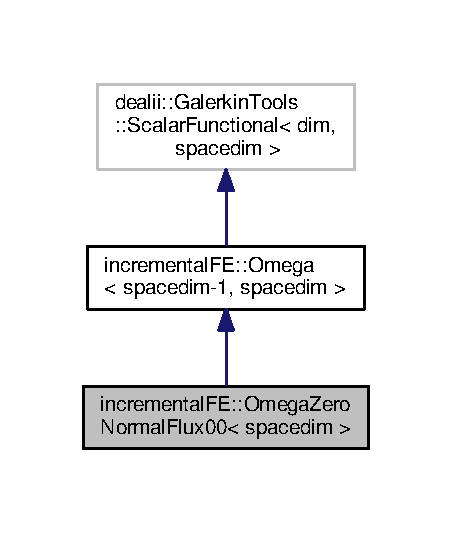
\includegraphics[width=217pt]{classincremental_f_e_1_1_omega_zero_normal_flux00__inherit__graph}
\end{center}
\end{figure}


Collaboration diagram for incremental\+FE\+:\+:Omega\+Zero\+Normal\+Flux00$<$ spacedim $>$\+:\nopagebreak
\begin{figure}[H]
\begin{center}
\leavevmode
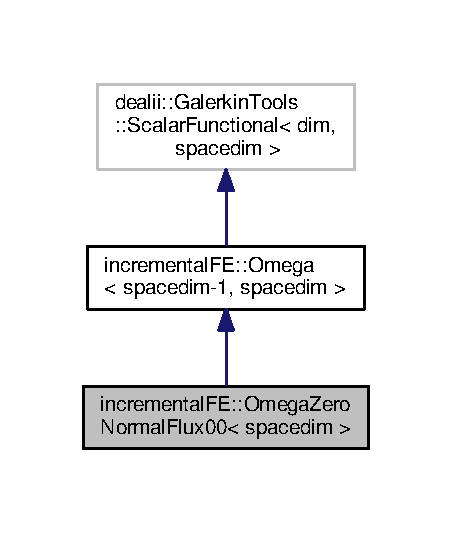
\includegraphics[width=217pt]{classincremental_f_e_1_1_omega_zero_normal_flux00__coll__graph}
\end{center}
\end{figure}
\subsection*{Public Member Functions}
\begin{DoxyCompactItemize}
\item 
\hyperlink{classincremental_f_e_1_1_omega_zero_normal_flux00_ae6b3992a1f7b54c41935c44115caafec}{Omega\+Zero\+Normal\+Flux00} (const std\+::vector$<$ dealii\+::\+Galerkin\+Tools\+::\+Dependent\+Field$<$ spacedim-\/1, spacedim $>$$>$ e\+\_\+sigma, const std\+::set$<$ {\bf dealii\+::types\+::material\+\_\+id} $>$ domain\+\_\+of\+\_\+integration, const dealii\+::\+Quadrature$<$ spacedim-\/1 $>$ quadrature, \hyperlink{classincremental_f_e_1_1_global_data_incremental_f_e}{Global\+Data\+Incremental\+FE}$<$ spacedim $>$ \&\hyperlink{classincremental_f_e_1_1_omega_abd23d288a7a4a43f9b528be968cd2113}{global\+\_\+data}, const unsigned int \hyperlink{classincremental_f_e_1_1_omega_a7600d263ebf98129629e44fa67e8a58c}{method}, const double \hyperlink{classincremental_f_e_1_1_omega_a891688560ec0ad8dc5a0058a7b400269}{alpha}=0.\+0)
\item 
bool \hyperlink{classincremental_f_e_1_1_omega_zero_normal_flux00_a2b27754a7083466923fe6eac25dfc0fd}{get\+\_\+values\+\_\+and\+\_\+derivatives} (const {\bf dealii\+::\+Vector}$<$ double $>$ \&{\bf values}, const double, const dealii\+::\+Point$<$ spacedim $>$ \&, const dealii\+::\+Tensor$<$ 1, spacedim $>$ \&n, double \&omega, {\bf dealii\+::\+Vector}$<$ double $>$ \&d\+\_\+omega, dealii\+::\+Full\+Matrix$<$ double $>$ \&d2\+\_\+omega, const std\+::tuple$<$ bool, bool, bool $>$ requested\+\_\+quantities, const bool) const 
\end{DoxyCompactItemize}
\subsection*{Additional Inherited Members}


\subsection{Detailed Description}
\subsubsection*{template$<$unsigned int spacedim$>$\\*
class incremental\+F\+E\+::\+Omega\+Zero\+Normal\+Flux00$<$ spacedim $>$}

Class defining an interface related scalar functional with the integrand

$ h^\Sigma_\tau = -\mu \dot{\boldsymbol{I}} \cdot \boldsymbol{n} $

where $\mu$ is a Lagrangian multiplier, and $\dot{\boldsymbol{I}}$ a flux.

This is meant to enforce a zero normal flux condition (e.\+g. for Raviart-\/\+Thomas finite elements).

Ordering of quantities in {\bf Scalar\+Functional\+::e\+\_\+sigma} \+:~\newline
\mbox{[}0\mbox{]} $I_x$~\newline
 \mbox{[}1\mbox{]} $I_y$~\newline
 \mbox{[}2\mbox{]} $I_z$~\newline
 \mbox{[}3\mbox{]} $\mu$~\newline
 

\subsection{Constructor \& Destructor Documentation}
\index{incremental\+F\+E\+::\+Omega\+Zero\+Normal\+Flux00@{incremental\+F\+E\+::\+Omega\+Zero\+Normal\+Flux00}!Omega\+Zero\+Normal\+Flux00@{Omega\+Zero\+Normal\+Flux00}}
\index{Omega\+Zero\+Normal\+Flux00@{Omega\+Zero\+Normal\+Flux00}!incremental\+F\+E\+::\+Omega\+Zero\+Normal\+Flux00@{incremental\+F\+E\+::\+Omega\+Zero\+Normal\+Flux00}}
\subsubsection[{\texorpdfstring{Omega\+Zero\+Normal\+Flux00(const std\+::vector$<$ dealii\+::\+Galerkin\+Tools\+::\+Dependent\+Field$<$ spacedim-\/1, spacedim $>$$>$ e\+\_\+sigma, const std\+::set$<$ dealii\+::types\+::material\+\_\+id $>$ domain\+\_\+of\+\_\+integration, const dealii\+::\+Quadrature$<$ spacedim-\/1 $>$ quadrature, Global\+Data\+Incremental\+F\+E$<$ spacedim $>$ \&global\+\_\+data, const unsigned int method, const double alpha=0.\+0)}{OmegaZeroNormalFlux00(const std::vector< dealii::GalerkinTools::DependentField< spacedim-1, spacedim >> e_sigma, const std::set< dealii::types::material_id > domain_of_integration, const dealii::Quadrature< spacedim-1 > quadrature, GlobalDataIncrementalFE< spacedim > &global_data, const unsigned int method, const double alpha=0.0)}}]{\setlength{\rightskip}{0pt plus 5cm}template$<$unsigned int spacedim$>$ {\bf incremental\+F\+E\+::\+Omega\+Zero\+Normal\+Flux00}$<$ spacedim $>$\+::{\bf Omega\+Zero\+Normal\+Flux00} (
\begin{DoxyParamCaption}
\item[{const std\+::vector$<$ dealii\+::\+Galerkin\+Tools\+::\+Dependent\+Field$<$ spacedim-\/1, spacedim $>$$>$}]{e\+\_\+sigma, }
\item[{const std\+::set$<$ {\bf dealii\+::types\+::material\+\_\+id} $>$}]{domain\+\_\+of\+\_\+integration, }
\item[{const dealii\+::\+Quadrature$<$ spacedim-\/1 $>$}]{quadrature, }
\item[{{\bf Global\+Data\+Incremental\+FE}$<$ spacedim $>$ \&}]{global\+\_\+data, }
\item[{const unsigned int}]{method, }
\item[{const double}]{alpha = {\ttfamily 0.0}}
\end{DoxyParamCaption}
)\hspace{0.3cm}{\ttfamily [inline]}}\hypertarget{classincremental_f_e_1_1_omega_zero_normal_flux00_ae6b3992a1f7b54c41935c44115caafec}{}\label{classincremental_f_e_1_1_omega_zero_normal_flux00_ae6b3992a1f7b54c41935c44115caafec}
Constructor


\begin{DoxyParams}[1]{Parameters}
\mbox{\tt in}  & {\em e\+\_\+sigma} & {\bf Scalar\+Functional\+::e\+\_\+sigma}\\
\hline
\mbox{\tt in}  & {\em domain\+\_\+of\+\_\+integration} & {\bf Scalar\+Functional\+::domain\+\_\+of\+\_\+integration}\\
\hline
\mbox{\tt in}  & {\em quadrature} & {\bf Scalar\+Functional\+::quadrature}\\
\hline
\mbox{\tt in}  & {\em global\+\_\+data} & \hyperlink{classincremental_f_e_1_1_omega_abd23d288a7a4a43f9b528be968cd2113}{Omega\+::global\+\_\+data}\\
\hline
\mbox{\tt in}  & {\em method} & \hyperlink{classincremental_f_e_1_1_omega_a7600d263ebf98129629e44fa67e8a58c}{Omega\+::method}\\
\hline
\mbox{\tt in}  & {\em alpha} & \hyperlink{classincremental_f_e_1_1_omega_a891688560ec0ad8dc5a0058a7b400269}{Omega\+::alpha} \\
\hline
\end{DoxyParams}


\subsection{Member Function Documentation}
\index{incremental\+F\+E\+::\+Omega\+Zero\+Normal\+Flux00@{incremental\+F\+E\+::\+Omega\+Zero\+Normal\+Flux00}!get\+\_\+values\+\_\+and\+\_\+derivatives@{get\+\_\+values\+\_\+and\+\_\+derivatives}}
\index{get\+\_\+values\+\_\+and\+\_\+derivatives@{get\+\_\+values\+\_\+and\+\_\+derivatives}!incremental\+F\+E\+::\+Omega\+Zero\+Normal\+Flux00@{incremental\+F\+E\+::\+Omega\+Zero\+Normal\+Flux00}}
\subsubsection[{\texorpdfstring{get\+\_\+values\+\_\+and\+\_\+derivatives(const dealii\+::\+Vector$<$ double $>$ \&values, const double, const dealii\+::\+Point$<$ spacedim $>$ \&, const dealii\+::\+Tensor$<$ 1, spacedim $>$ \&n, double \&omega, dealii\+::\+Vector$<$ double $>$ \&d\+\_\+omega, dealii\+::\+Full\+Matrix$<$ double $>$ \&d2\+\_\+omega, const std\+::tuple$<$ bool, bool, bool $>$ requested\+\_\+quantities, const bool) const }{get_values_and_derivatives(const dealii::Vector< double > &values, const double, const dealii::Point< spacedim > &, const dealii::Tensor< 1, spacedim > &n, double &omega, dealii::Vector< double > &d_omega, dealii::FullMatrix< double > &d2_omega, const std::tuple< bool, bool, bool > requested_quantities, const bool) const }}]{\setlength{\rightskip}{0pt plus 5cm}template$<$unsigned int spacedim$>$ bool {\bf incremental\+F\+E\+::\+Omega\+Zero\+Normal\+Flux00}$<$ spacedim $>$\+::get\+\_\+values\+\_\+and\+\_\+derivatives (
\begin{DoxyParamCaption}
\item[{const {\bf dealii\+::\+Vector}$<$ double $>$ \&}]{values, }
\item[{const double}]{, }
\item[{const dealii\+::\+Point$<$ spacedim $>$ \&}]{, }
\item[{const dealii\+::\+Tensor$<$ 1, spacedim $>$ \&}]{n, }
\item[{double \&}]{omega, }
\item[{{\bf dealii\+::\+Vector}$<$ double $>$ \&}]{d\+\_\+omega, }
\item[{dealii\+::\+Full\+Matrix$<$ double $>$ \&}]{d2\+\_\+omega, }
\item[{const std\+::tuple$<$ bool, bool, bool $>$}]{requested\+\_\+quantities, }
\item[{const bool}]{}
\end{DoxyParamCaption}
) const\hspace{0.3cm}{\ttfamily [inline]}, {\ttfamily [virtual]}}\hypertarget{classincremental_f_e_1_1_omega_zero_normal_flux00_a2b27754a7083466923fe6eac25dfc0fd}{}\label{classincremental_f_e_1_1_omega_zero_normal_flux00_a2b27754a7083466923fe6eac25dfc0fd}
\begin{DoxySeeAlso}{See also}
\hyperlink{classincremental_f_e_1_1_omega_a2f35d862aefa11151de5b7c7411e45df}{Omega\+::get\+\_\+values\+\_\+and\+\_\+derivatives()} 
\end{DoxySeeAlso}


Implements \hyperlink{classincremental_f_e_1_1_omega_a2f35d862aefa11151de5b7c7411e45df}{incremental\+F\+E\+::\+Omega$<$ spacedim-\/1, spacedim $>$}.



The documentation for this class was generated from the following file\+:\begin{DoxyCompactItemize}
\item 
/home/sst/code/\+Incremental\+F\+E/\+Incremental\+F\+E/include/incremental\+\_\+fe/scalar\+\_\+functionals/\hyperlink{omega__lib_8h}{omega\+\_\+lib.\+h}\end{DoxyCompactItemize}

\hypertarget{classincremental_f_e_1_1_psi}{}\section{incremental\+FE\+:\+:Psi$<$ dim, spacedim $>$ Class Template Reference}
\label{classincremental_f_e_1_1_psi}\index{incremental\+F\+E\+::\+Psi$<$ dim, spacedim $>$@{incremental\+F\+E\+::\+Psi$<$ dim, spacedim $>$}}


{\ttfamily \#include $<$psi.\+h$>$}



Inheritance diagram for incremental\+FE\+:\+:Psi$<$ dim, spacedim $>$\+:\nopagebreak
\begin{figure}[H]
\begin{center}
\leavevmode
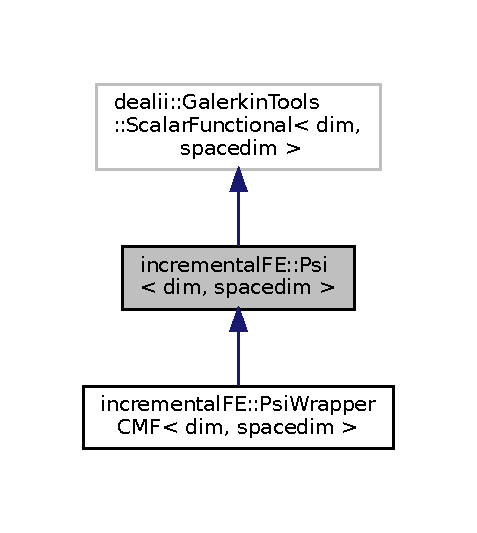
\includegraphics[width=203pt]{classincremental_f_e_1_1_psi__inherit__graph}
\end{center}
\end{figure}


Collaboration diagram for incremental\+FE\+:\+:Psi$<$ dim, spacedim $>$\+:\nopagebreak
\begin{figure}[H]
\begin{center}
\leavevmode
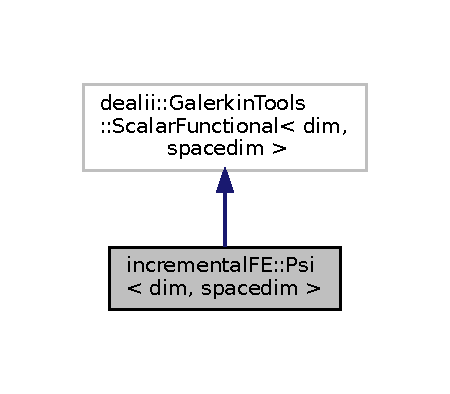
\includegraphics[width=203pt]{classincremental_f_e_1_1_psi__coll__graph}
\end{center}
\end{figure}
\subsection*{Public Member Functions}
\begin{DoxyCompactItemize}
\item 
\hyperlink{classincremental_f_e_1_1_psi_ae8a4aab5ee5381799379b8de2bc1f67d}{Psi} (const std\+::vector$<$ dealii\+::\+Galerkin\+Tools\+::\+Dependent\+Field$<$ dim, spacedim $>$$>$ e\+\_\+sigma, const std\+::set$<$ {\bf dealii\+::types\+::material\+\_\+id} $>$ domain\+\_\+of\+\_\+integration, const dealii\+::\+Quadrature$<$ dim $>$ quadrature, \hyperlink{classincremental_f_e_1_1_global_data_incremental_f_e}{Global\+Data\+Incremental\+FE}$<$ spacedim $>$ \&\hyperlink{classincremental_f_e_1_1_psi_ae77b2e13385734b19d6ee445c477a6eb}{global\+\_\+data}, const double \hyperlink{classincremental_f_e_1_1_psi_a0d59fde4728962fa75449a3444341dcf}{alpha}=0.\+0, const std\+::string name=\char`\"{}Psi\char`\"{})
\item 
virtual \hyperlink{classincremental_f_e_1_1_psi_a22a7b3d4fd98f6d0cff79623e13e0939}{$\sim$\+Psi} ()=default
\item 
virtual bool \hyperlink{classincremental_f_e_1_1_psi_a2622e8f84590e8a821984181e31fbc76}{get\+\_\+values\+\_\+and\+\_\+derivatives} (const {\bf dealii\+::\+Vector}$<$ double $>$ \&{\bf values}, const dealii\+::\+Point$<$ spacedim $>$ \&x, const dealii\+::\+Tensor$<$ 1, spacedim $>$ \&n, double \&psi, {\bf dealii\+::\+Vector}$<$ double $>$ \&d\+\_\+psi, dealii\+::\+Full\+Matrix$<$ double $>$ \&d2\+\_\+psi, const std\+::tuple$<$ bool, bool, bool $>$ requested\+\_\+quantities) const =0
\item 
bool \hyperlink{classincremental_f_e_1_1_psi_ab4e1abcaff9497eac5eb3c953f2c303a}{get\+\_\+h\+\_\+sigma} (const {\bf dealii\+::\+Vector}$<$ double $>$ \&e\+\_\+sigma, const std\+::vector$<$ {\bf dealii\+::\+Vector}$<$ double $>$$>$ \&e\+\_\+sigma\+\_\+ref\+\_\+sets, {\bf dealii\+::\+Vector}$<$ double $>$ \&hidden\+\_\+vars, const dealii\+::\+Point$<$ spacedim $>$ \&x, const dealii\+::\+Tensor$<$ 1, spacedim $>$ \&n, double \&h\+\_\+sigma, {\bf dealii\+::\+Vector}$<$ double $>$ \&h\+\_\+sigma\+\_\+1, dealii\+::\+Full\+Matrix$<$ double $>$ \&h\+\_\+sigma\+\_\+2, const std\+::tuple$<$ bool, bool, bool $>$ requested\+\_\+quantities) const final
\end{DoxyCompactItemize}
\subsection*{Private Attributes}
\begin{DoxyCompactItemize}
\item 
const dealii\+::\+Smart\+Pointer$<$ \hyperlink{classincremental_f_e_1_1_global_data_incremental_f_e}{Global\+Data\+Incremental\+FE}$<$ spacedim $>$ $>$ \hyperlink{classincremental_f_e_1_1_psi_ae77b2e13385734b19d6ee445c477a6eb}{global\+\_\+data}
\item 
const double \hyperlink{classincremental_f_e_1_1_psi_a0d59fde4728962fa75449a3444341dcf}{alpha}
\end{DoxyCompactItemize}


\subsection{Detailed Description}
\subsubsection*{template$<$unsigned int dim, unsigned int spacedim$>$\\*
class incremental\+F\+E\+::\+Psi$<$ dim, spacedim $>$}

Class defining an interface related scalar functional with the integrand

$ h^\Sigma_\tau = \alpha \psi(q_{n+1}) + (1-\alpha) \left[ \psi(q_n) + \psi_q(q_n) (q_{n+1} - q_n)\right] $,

where $0\leq \alpha \leq 1 $ is a numerical parameter, and $q_n$ and $q_{n+1}$ is the value of the state variable $q$ in the beginning of the time step and at the end of the time step, respectively. $q$ can also be vector valued. 

\subsection{Constructor \& Destructor Documentation}
\index{incremental\+F\+E\+::\+Psi@{incremental\+F\+E\+::\+Psi}!Psi@{Psi}}
\index{Psi@{Psi}!incremental\+F\+E\+::\+Psi@{incremental\+F\+E\+::\+Psi}}
\subsubsection[{\texorpdfstring{Psi(const std\+::vector$<$ dealii\+::\+Galerkin\+Tools\+::\+Dependent\+Field$<$ dim, spacedim $>$$>$ e\+\_\+sigma, const std\+::set$<$ dealii\+::types\+::material\+\_\+id $>$ domain\+\_\+of\+\_\+integration, const dealii\+::\+Quadrature$<$ dim $>$ quadrature, Global\+Data\+Incremental\+F\+E$<$ spacedim $>$ \&global\+\_\+data, const double alpha=0.\+0, const std\+::string name=""Psi"")}{Psi(const std::vector< dealii::GalerkinTools::DependentField< dim, spacedim >> e_sigma, const std::set< dealii::types::material_id > domain_of_integration, const dealii::Quadrature< dim > quadrature, GlobalDataIncrementalFE< spacedim > &global_data, const double alpha=0.0, const std::string name="Psi")}}]{\setlength{\rightskip}{0pt plus 5cm}template$<$unsigned int dim, unsigned int spacedim$>$ {\bf incremental\+F\+E\+::\+Psi}$<$ dim, spacedim $>$\+::{\bf Psi} (
\begin{DoxyParamCaption}
\item[{const std\+::vector$<$ dealii\+::\+Galerkin\+Tools\+::\+Dependent\+Field$<$ dim, spacedim $>$$>$}]{e\+\_\+sigma, }
\item[{const std\+::set$<$ {\bf dealii\+::types\+::material\+\_\+id} $>$}]{domain\+\_\+of\+\_\+integration, }
\item[{const dealii\+::\+Quadrature$<$ dim $>$}]{quadrature, }
\item[{{\bf Global\+Data\+Incremental\+FE}$<$ spacedim $>$ \&}]{global\+\_\+data, }
\item[{const double}]{alpha = {\ttfamily 0.0}, }
\item[{const std\+::string}]{name = {\ttfamily \char`\"{}Psi$<$~dim,~spacedim~$>$\char`\"{}}}
\end{DoxyParamCaption}
)}\hypertarget{classincremental_f_e_1_1_psi_ae8a4aab5ee5381799379b8de2bc1f67d}{}\label{classincremental_f_e_1_1_psi_ae8a4aab5ee5381799379b8de2bc1f67d}
Constructor


\begin{DoxyParams}[1]{Parameters}
\mbox{\tt in}  & {\em e\+\_\+sigma} & Dependent fields $q$\\
\hline
\mbox{\tt in}  & {\em domain\+\_\+of\+\_\+integration} & {\bf Scalar\+Functional\+::domain\+\_\+of\+\_\+integration}\\
\hline
\mbox{\tt in}  & {\em quadrature} & {\bf Scalar\+Functional\+::quadrature}\\
\hline
\mbox{\tt in}  & {\em global\+\_\+data} & \hyperlink{classincremental_f_e_1_1_psi_ae77b2e13385734b19d6ee445c477a6eb}{Psi\+::global\+\_\+data}\\
\hline
\mbox{\tt in}  & {\em alpha} & \hyperlink{classincremental_f_e_1_1_psi_a0d59fde4728962fa75449a3444341dcf}{Psi\+::alpha}\\
\hline
\mbox{\tt in}  & {\em name} & {\bf Scalar\+Functional\+::name} \\
\hline
\end{DoxyParams}
\index{incremental\+F\+E\+::\+Psi@{incremental\+F\+E\+::\+Psi}!````~Psi@{$\sim$\+Psi}}
\index{````~Psi@{$\sim$\+Psi}!incremental\+F\+E\+::\+Psi@{incremental\+F\+E\+::\+Psi}}
\subsubsection[{\texorpdfstring{$\sim$\+Psi()=default}{~Psi()=default}}]{\setlength{\rightskip}{0pt plus 5cm}template$<$unsigned int dim, unsigned int spacedim$>$ virtual {\bf incremental\+F\+E\+::\+Psi}$<$ dim, spacedim $>$\+::$\sim${\bf Psi} (
\begin{DoxyParamCaption}
{}
\end{DoxyParamCaption}
)\hspace{0.3cm}{\ttfamily [virtual]}, {\ttfamily [default]}}\hypertarget{classincremental_f_e_1_1_psi_a22a7b3d4fd98f6d0cff79623e13e0939}{}\label{classincremental_f_e_1_1_psi_a22a7b3d4fd98f6d0cff79623e13e0939}
Destructor 

\subsection{Member Function Documentation}
\index{incremental\+F\+E\+::\+Psi@{incremental\+F\+E\+::\+Psi}!get\+\_\+h\+\_\+sigma@{get\+\_\+h\+\_\+sigma}}
\index{get\+\_\+h\+\_\+sigma@{get\+\_\+h\+\_\+sigma}!incremental\+F\+E\+::\+Psi@{incremental\+F\+E\+::\+Psi}}
\subsubsection[{\texorpdfstring{get\+\_\+h\+\_\+sigma(const dealii\+::\+Vector$<$ double $>$ \&e\+\_\+sigma, const std\+::vector$<$ dealii\+::\+Vector$<$ double $>$$>$ \&e\+\_\+sigma\+\_\+ref\+\_\+sets, dealii\+::\+Vector$<$ double $>$ \&hidden\+\_\+vars, const dealii\+::\+Point$<$ spacedim $>$ \&x, const dealii\+::\+Tensor$<$ 1, spacedim $>$ \&n, double \&h\+\_\+sigma, dealii\+::\+Vector$<$ double $>$ \&h\+\_\+sigma\+\_\+1, dealii\+::\+Full\+Matrix$<$ double $>$ \&h\+\_\+sigma\+\_\+2, const std\+::tuple$<$ bool, bool, bool $>$ requested\+\_\+quantities) const final}{get_h_sigma(const dealii::Vector< double > &e_sigma, const std::vector< dealii::Vector< double >> &e_sigma_ref_sets, dealii::Vector< double > &hidden_vars, const dealii::Point< spacedim > &x, const dealii::Tensor< 1, spacedim > &n, double &h_sigma, dealii::Vector< double > &h_sigma_1, dealii::FullMatrix< double > &h_sigma_2, const std::tuple< bool, bool, bool > requested_quantities) const final}}]{\setlength{\rightskip}{0pt plus 5cm}template$<$unsigned int dim, unsigned int spacedim$>$ bool {\bf incremental\+F\+E\+::\+Psi}$<$ dim, spacedim $>$\+::get\+\_\+h\+\_\+sigma (
\begin{DoxyParamCaption}
\item[{const {\bf dealii\+::\+Vector}$<$ double $>$ \&}]{e\+\_\+sigma, }
\item[{const std\+::vector$<$ {\bf dealii\+::\+Vector}$<$ double $>$$>$ \&}]{e\+\_\+sigma\+\_\+ref\+\_\+sets, }
\item[{{\bf dealii\+::\+Vector}$<$ double $>$ \&}]{hidden\+\_\+vars, }
\item[{const dealii\+::\+Point$<$ spacedim $>$ \&}]{x, }
\item[{const dealii\+::\+Tensor$<$ 1, spacedim $>$ \&}]{n, }
\item[{double \&}]{h\+\_\+sigma, }
\item[{{\bf dealii\+::\+Vector}$<$ double $>$ \&}]{h\+\_\+sigma\+\_\+1, }
\item[{dealii\+::\+Full\+Matrix$<$ double $>$ \&}]{h\+\_\+sigma\+\_\+2, }
\item[{const std\+::tuple$<$ bool, bool, bool $>$}]{requested\+\_\+quantities}
\end{DoxyParamCaption}
) const\hspace{0.3cm}{\ttfamily [final]}}\hypertarget{classincremental_f_e_1_1_psi_ab4e1abcaff9497eac5eb3c953f2c303a}{}\label{classincremental_f_e_1_1_psi_ab4e1abcaff9497eac5eb3c953f2c303a}
see {\bf Scalar\+Functional\+::get\+\_\+h\+\_\+sigma} \index{incremental\+F\+E\+::\+Psi@{incremental\+F\+E\+::\+Psi}!get\+\_\+values\+\_\+and\+\_\+derivatives@{get\+\_\+values\+\_\+and\+\_\+derivatives}}
\index{get\+\_\+values\+\_\+and\+\_\+derivatives@{get\+\_\+values\+\_\+and\+\_\+derivatives}!incremental\+F\+E\+::\+Psi@{incremental\+F\+E\+::\+Psi}}
\subsubsection[{\texorpdfstring{get\+\_\+values\+\_\+and\+\_\+derivatives(const dealii\+::\+Vector$<$ double $>$ \&values, const dealii\+::\+Point$<$ spacedim $>$ \&x, const dealii\+::\+Tensor$<$ 1, spacedim $>$ \&n, double \&psi, dealii\+::\+Vector$<$ double $>$ \&d\+\_\+psi, dealii\+::\+Full\+Matrix$<$ double $>$ \&d2\+\_\+psi, const std\+::tuple$<$ bool, bool, bool $>$ requested\+\_\+quantities) const =0}{get_values_and_derivatives(const dealii::Vector< double > &values, const dealii::Point< spacedim > &x, const dealii::Tensor< 1, spacedim > &n, double &psi, dealii::Vector< double > &d_psi, dealii::FullMatrix< double > &d2_psi, const std::tuple< bool, bool, bool > requested_quantities) const =0}}]{\setlength{\rightskip}{0pt plus 5cm}template$<$unsigned int dim, unsigned int spacedim$>$ virtual bool {\bf incremental\+F\+E\+::\+Psi}$<$ dim, spacedim $>$\+::get\+\_\+values\+\_\+and\+\_\+derivatives (
\begin{DoxyParamCaption}
\item[{const {\bf dealii\+::\+Vector}$<$ double $>$ \&}]{values, }
\item[{const dealii\+::\+Point$<$ spacedim $>$ \&}]{x, }
\item[{const dealii\+::\+Tensor$<$ 1, spacedim $>$ \&}]{n, }
\item[{double \&}]{psi, }
\item[{{\bf dealii\+::\+Vector}$<$ double $>$ \&}]{d\+\_\+psi, }
\item[{dealii\+::\+Full\+Matrix$<$ double $>$ \&}]{d2\+\_\+psi, }
\item[{const std\+::tuple$<$ bool, bool, bool $>$}]{requested\+\_\+quantities}
\end{DoxyParamCaption}
) const\hspace{0.3cm}{\ttfamily [pure virtual]}}\hypertarget{classincremental_f_e_1_1_psi_a2622e8f84590e8a821984181e31fbc76}{}\label{classincremental_f_e_1_1_psi_a2622e8f84590e8a821984181e31fbc76}
This function defines $\psi(q)$ and needs to be implemented by classes inheriting from this class


\begin{DoxyParams}[1]{Parameters}
\mbox{\tt in}  & {\em values} & Values at which $\psi$ and its derivatives are evaluated\\
\hline
\mbox{\tt in}  & {\em x} & Position\\
\hline
\mbox{\tt in}  & {\em n} & Normal vector\\
\hline
\mbox{\tt out}  & {\em psi} & Value of $\psi$\\
\hline
\mbox{\tt out}  & {\em d\+\_\+psi} & Values of first derivatives of $\psi$ w.\+r.\+t. $q$\\
\hline
\mbox{\tt out}  & {\em d2\+\_\+psi} & Values of second derivatives of $\psi$ w.\+r.\+t. $q$\\
\hline
\mbox{\tt in}  & {\em requested\+\_\+quantities} & Tuple indicating which of the quantities {\ttfamily psi}, {\ttfamily d\+\_\+psi}, {\ttfamily d2\+\_\+psi} are to be computed (note that only those quantities are initialized to the correct size, which are actually requested).\\
\hline
\end{DoxyParams}
\begin{DoxyReturn}{Returns}
{\ttfamily true} indicates that an error has occurred in the function 
\end{DoxyReturn}


\subsection{Member Data Documentation}
\index{incremental\+F\+E\+::\+Psi@{incremental\+F\+E\+::\+Psi}!alpha@{alpha}}
\index{alpha@{alpha}!incremental\+F\+E\+::\+Psi@{incremental\+F\+E\+::\+Psi}}
\subsubsection[{\texorpdfstring{alpha}{alpha}}]{\setlength{\rightskip}{0pt plus 5cm}template$<$unsigned int dim, unsigned int spacedim$>$ const double {\bf incremental\+F\+E\+::\+Psi}$<$ dim, spacedim $>$\+::alpha\hspace{0.3cm}{\ttfamily [private]}}\hypertarget{classincremental_f_e_1_1_psi_a0d59fde4728962fa75449a3444341dcf}{}\label{classincremental_f_e_1_1_psi_a0d59fde4728962fa75449a3444341dcf}
Numerical parameter between {\ttfamily 0} and {\ttfamily 1}. \index{incremental\+F\+E\+::\+Psi@{incremental\+F\+E\+::\+Psi}!global\+\_\+data@{global\+\_\+data}}
\index{global\+\_\+data@{global\+\_\+data}!incremental\+F\+E\+::\+Psi@{incremental\+F\+E\+::\+Psi}}
\subsubsection[{\texorpdfstring{global\+\_\+data}{global_data}}]{\setlength{\rightskip}{0pt plus 5cm}template$<$unsigned int dim, unsigned int spacedim$>$ const dealii\+::\+Smart\+Pointer$<${\bf Global\+Data\+Incremental\+FE}$<$spacedim$>$ $>$ {\bf incremental\+F\+E\+::\+Psi}$<$ dim, spacedim $>$\+::global\+\_\+data\hspace{0.3cm}{\ttfamily [private]}}\hypertarget{classincremental_f_e_1_1_psi_ae77b2e13385734b19d6ee445c477a6eb}{}\label{classincremental_f_e_1_1_psi_ae77b2e13385734b19d6ee445c477a6eb}
global data object 

The documentation for this class was generated from the following file\+:\begin{DoxyCompactItemize}
\item 
/home/sst/code/\+Incremental\+F\+E/\+Incremental\+F\+E/include/incremental\+\_\+fe/scalar\+\_\+functionals/\hyperlink{psi_8h}{psi.\+h}\end{DoxyCompactItemize}

\hypertarget{classincremental_f_e_1_1_psi_3_01spacedim_00_01spacedim_01_4}{}\section{incremental\+FE\+:\+:Psi$<$ spacedim, spacedim $>$ Class Template Reference}
\label{classincremental_f_e_1_1_psi_3_01spacedim_00_01spacedim_01_4}\index{incremental\+F\+E\+::\+Psi$<$ spacedim, spacedim $>$@{incremental\+F\+E\+::\+Psi$<$ spacedim, spacedim $>$}}


{\ttfamily \#include $<$psi.\+h$>$}



Inheritance diagram for incremental\+FE\+:\+:Psi$<$ spacedim, spacedim $>$\+:\nopagebreak
\begin{figure}[H]
\begin{center}
\leavevmode
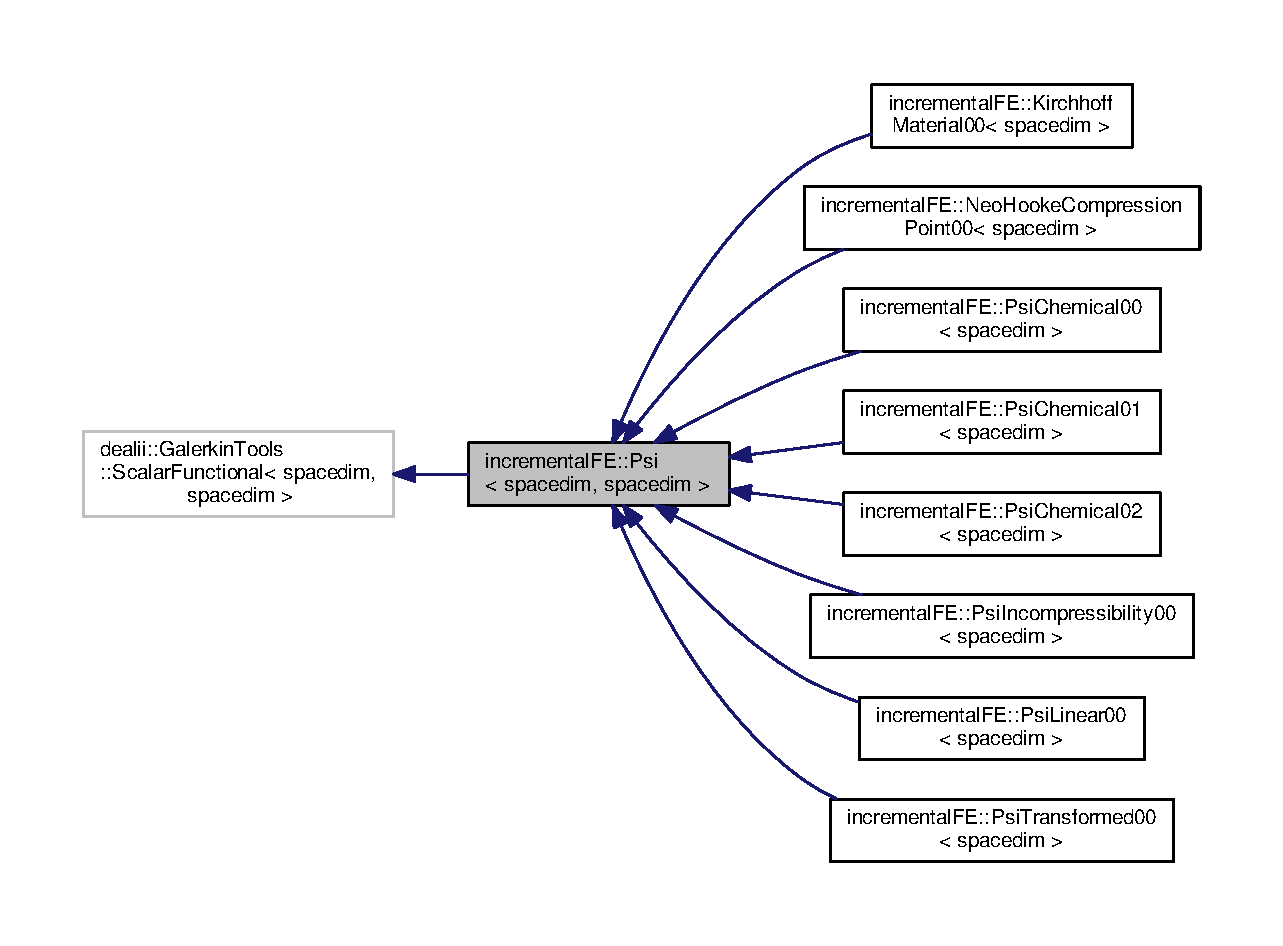
\includegraphics[width=350pt]{classincremental_f_e_1_1_psi_3_01spacedim_00_01spacedim_01_4__inherit__graph}
\end{center}
\end{figure}


Collaboration diagram for incremental\+FE\+:\+:Psi$<$ spacedim, spacedim $>$\+:\nopagebreak
\begin{figure}[H]
\begin{center}
\leavevmode
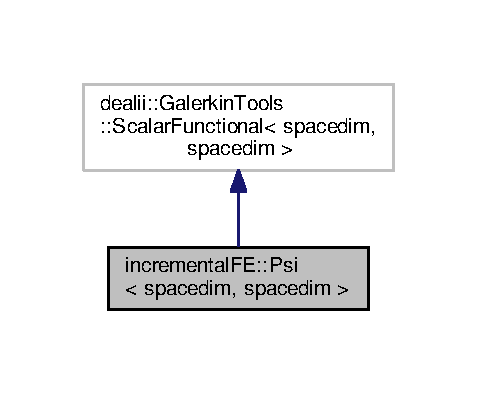
\includegraphics[width=229pt]{classincremental_f_e_1_1_psi_3_01spacedim_00_01spacedim_01_4__coll__graph}
\end{center}
\end{figure}
\subsection*{Public Member Functions}
\begin{DoxyCompactItemize}
\item 
\hyperlink{classincremental_f_e_1_1_psi_3_01spacedim_00_01spacedim_01_4_ad6aff88570ea114f34ca92f232759e29}{Psi} (const std\+::vector$<$ dealii\+::\+Galerkin\+Tools\+::\+Dependent\+Field$<$ spacedim, spacedim $>$$>$ e\+\_\+omega, const std\+::set$<$ {\bf dealii\+::types\+::material\+\_\+id} $>$ domain\+\_\+of\+\_\+integration, const dealii\+::\+Quadrature$<$ spacedim $>$ quadrature, \hyperlink{classincremental_f_e_1_1_global_data_incremental_f_e}{Global\+Data\+Incremental\+FE}$<$ spacedim $>$ \&\hyperlink{classincremental_f_e_1_1_psi_3_01spacedim_00_01spacedim_01_4_abf0a4804877fd7cc9bd1b90e52760ba9}{global\+\_\+data}, const double \hyperlink{classincremental_f_e_1_1_psi_3_01spacedim_00_01spacedim_01_4_af7b8227188dbdd6ada35b9445d96c79d}{alpha}=0.\+0, const std\+::string name=\char`\"{}Psi\char`\"{})
\item 
virtual \hyperlink{classincremental_f_e_1_1_psi_3_01spacedim_00_01spacedim_01_4_a9e215c6ac92f535204bd35ebe0593125}{$\sim$\+Psi} ()=default
\item 
virtual bool \hyperlink{classincremental_f_e_1_1_psi_3_01spacedim_00_01spacedim_01_4_a17f3559c196edb5487b591bb6061667e}{get\+\_\+values\+\_\+and\+\_\+derivatives} (const {\bf dealii\+::\+Vector}$<$ double $>$ \&{\bf values}, const dealii\+::\+Point$<$ spacedim $>$ \&x, double \&psi, {\bf dealii\+::\+Vector}$<$ double $>$ \&d\+\_\+psi, dealii\+::\+Full\+Matrix$<$ double $>$ \&d2\+\_\+psi, const std\+::tuple$<$ bool, bool, bool $>$ requested\+\_\+quantities) const =0
\item 
bool \hyperlink{classincremental_f_e_1_1_psi_3_01spacedim_00_01spacedim_01_4_ac4ea5fab83e51805dc405517cb35570b}{get\+\_\+h\+\_\+omega} (const {\bf dealii\+::\+Vector}$<$ double $>$ \&e\+\_\+omega, const std\+::vector$<$ {\bf dealii\+::\+Vector}$<$ double $>$$>$ \&e\+\_\+omega\+\_\+ref\+\_\+sets, {\bf dealii\+::\+Vector}$<$ double $>$ \&hidden\+\_\+vars, const dealii\+::\+Point$<$ spacedim $>$ \&x, double \&h\+\_\+omega, {\bf dealii\+::\+Vector}$<$ double $>$ \&h\+\_\+omega\+\_\+1, dealii\+::\+Full\+Matrix$<$ double $>$ \&h\+\_\+omega\+\_\+2, const std\+::tuple$<$ bool, bool, bool $>$ requested\+\_\+quantities) const final
\end{DoxyCompactItemize}
\subsection*{Private Attributes}
\begin{DoxyCompactItemize}
\item 
const dealii\+::\+Smart\+Pointer$<$ \hyperlink{classincremental_f_e_1_1_global_data_incremental_f_e}{Global\+Data\+Incremental\+FE}$<$ spacedim $>$ $>$ \hyperlink{classincremental_f_e_1_1_psi_3_01spacedim_00_01spacedim_01_4_abf0a4804877fd7cc9bd1b90e52760ba9}{global\+\_\+data}
\item 
const double \hyperlink{classincremental_f_e_1_1_psi_3_01spacedim_00_01spacedim_01_4_af7b8227188dbdd6ada35b9445d96c79d}{alpha}
\end{DoxyCompactItemize}


\subsection{Detailed Description}
\subsubsection*{template$<$unsigned int spacedim$>$\\*
class incremental\+F\+E\+::\+Psi$<$ spacedim, spacedim $>$}

Class defining a domain related scalar functional with the integrand

$ h^\Omega_\rho = \alpha \psi(q_{n+1}) + (1-\alpha) \left[ \psi(q_n) + \psi_q(q_n) (q_{n+1} - q_n)\right] $,

where $0\leq \alpha \leq 1 $ is a numerical parameter, and $q_n$ and $q_{n+1}$ is the value of the state variable $q$ in the beginning of the time step and at the end of the time step, respectively. $q$ can also be vector valued. 

\subsection{Constructor \& Destructor Documentation}
\index{incremental\+F\+E\+::\+Psi$<$ spacedim, spacedim $>$@{incremental\+F\+E\+::\+Psi$<$ spacedim, spacedim $>$}!Psi@{Psi}}
\index{Psi@{Psi}!incremental\+F\+E\+::\+Psi$<$ spacedim, spacedim $>$@{incremental\+F\+E\+::\+Psi$<$ spacedim, spacedim $>$}}
\subsubsection[{\texorpdfstring{Psi(const std\+::vector$<$ dealii\+::\+Galerkin\+Tools\+::\+Dependent\+Field$<$ spacedim, spacedim $>$$>$ e\+\_\+omega, const std\+::set$<$ dealii\+::types\+::material\+\_\+id $>$ domain\+\_\+of\+\_\+integration, const dealii\+::\+Quadrature$<$ spacedim $>$ quadrature, Global\+Data\+Incremental\+F\+E$<$ spacedim $>$ \&global\+\_\+data, const double alpha=0.\+0, const std\+::string name=""Psi"")}{Psi(const std::vector< dealii::GalerkinTools::DependentField< spacedim, spacedim >> e_omega, const std::set< dealii::types::material_id > domain_of_integration, const dealii::Quadrature< spacedim > quadrature, GlobalDataIncrementalFE< spacedim > &global_data, const double alpha=0.0, const std::string name="Psi")}}]{\setlength{\rightskip}{0pt plus 5cm}template$<$unsigned int spacedim$>$ {\bf incremental\+F\+E\+::\+Psi}$<$ spacedim, spacedim $>$\+::{\bf Psi} (
\begin{DoxyParamCaption}
\item[{const std\+::vector$<$ dealii\+::\+Galerkin\+Tools\+::\+Dependent\+Field$<$ spacedim, spacedim $>$$>$}]{e\+\_\+omega, }
\item[{const std\+::set$<$ {\bf dealii\+::types\+::material\+\_\+id} $>$}]{domain\+\_\+of\+\_\+integration, }
\item[{const dealii\+::\+Quadrature$<$ spacedim $>$}]{quadrature, }
\item[{{\bf Global\+Data\+Incremental\+FE}$<$ spacedim $>$ \&}]{global\+\_\+data, }
\item[{const double}]{alpha = {\ttfamily 0.0}, }
\item[{const std\+::string}]{name = {\ttfamily \char`\"{}Psi$<$~spacedim,~spacedim~$>$\char`\"{}}}
\end{DoxyParamCaption}
)}\hypertarget{classincremental_f_e_1_1_psi_3_01spacedim_00_01spacedim_01_4_ad6aff88570ea114f34ca92f232759e29}{}\label{classincremental_f_e_1_1_psi_3_01spacedim_00_01spacedim_01_4_ad6aff88570ea114f34ca92f232759e29}
Constructor


\begin{DoxyParams}[1]{Parameters}
\mbox{\tt in}  & {\em e\+\_\+omega} & Dependent fields $q$\\
\hline
\mbox{\tt in}  & {\em domain\+\_\+of\+\_\+integration} & {\bf Scalar\+Functional\+::domain\+\_\+of\+\_\+integration}\\
\hline
\mbox{\tt in}  & {\em quadrature} & {\bf Scalar\+Functional\+::quadrature}\\
\hline
\mbox{\tt in}  & {\em global\+\_\+data} & \hyperlink{classincremental_f_e_1_1_psi_ae77b2e13385734b19d6ee445c477a6eb}{Psi\+::global\+\_\+data}\\
\hline
\mbox{\tt in}  & {\em alpha} & \hyperlink{classincremental_f_e_1_1_psi_a0d59fde4728962fa75449a3444341dcf}{Psi\+::alpha}\\
\hline
\mbox{\tt in}  & {\em name} & {\bf Scalar\+Functional\+::name} \\
\hline
\end{DoxyParams}
\index{incremental\+F\+E\+::\+Psi$<$ spacedim, spacedim $>$@{incremental\+F\+E\+::\+Psi$<$ spacedim, spacedim $>$}!````~Psi@{$\sim$\+Psi}}
\index{````~Psi@{$\sim$\+Psi}!incremental\+F\+E\+::\+Psi$<$ spacedim, spacedim $>$@{incremental\+F\+E\+::\+Psi$<$ spacedim, spacedim $>$}}
\subsubsection[{\texorpdfstring{$\sim$\+Psi()=default}{~Psi()=default}}]{\setlength{\rightskip}{0pt plus 5cm}template$<$unsigned int spacedim$>$ virtual {\bf incremental\+F\+E\+::\+Psi}$<$ spacedim, spacedim $>$\+::$\sim${\bf Psi} (
\begin{DoxyParamCaption}
{}
\end{DoxyParamCaption}
)\hspace{0.3cm}{\ttfamily [virtual]}, {\ttfamily [default]}}\hypertarget{classincremental_f_e_1_1_psi_3_01spacedim_00_01spacedim_01_4_a9e215c6ac92f535204bd35ebe0593125}{}\label{classincremental_f_e_1_1_psi_3_01spacedim_00_01spacedim_01_4_a9e215c6ac92f535204bd35ebe0593125}
Destructor 

\subsection{Member Function Documentation}
\index{incremental\+F\+E\+::\+Psi$<$ spacedim, spacedim $>$@{incremental\+F\+E\+::\+Psi$<$ spacedim, spacedim $>$}!get\+\_\+h\+\_\+omega@{get\+\_\+h\+\_\+omega}}
\index{get\+\_\+h\+\_\+omega@{get\+\_\+h\+\_\+omega}!incremental\+F\+E\+::\+Psi$<$ spacedim, spacedim $>$@{incremental\+F\+E\+::\+Psi$<$ spacedim, spacedim $>$}}
\subsubsection[{\texorpdfstring{get\+\_\+h\+\_\+omega(const dealii\+::\+Vector$<$ double $>$ \&e\+\_\+omega, const std\+::vector$<$ dealii\+::\+Vector$<$ double $>$$>$ \&e\+\_\+omega\+\_\+ref\+\_\+sets, dealii\+::\+Vector$<$ double $>$ \&hidden\+\_\+vars, const dealii\+::\+Point$<$ spacedim $>$ \&x, double \&h\+\_\+omega, dealii\+::\+Vector$<$ double $>$ \&h\+\_\+omega\+\_\+1, dealii\+::\+Full\+Matrix$<$ double $>$ \&h\+\_\+omega\+\_\+2, const std\+::tuple$<$ bool, bool, bool $>$ requested\+\_\+quantities) const final}{get_h_omega(const dealii::Vector< double > &e_omega, const std::vector< dealii::Vector< double >> &e_omega_ref_sets, dealii::Vector< double > &hidden_vars, const dealii::Point< spacedim > &x, double &h_omega, dealii::Vector< double > &h_omega_1, dealii::FullMatrix< double > &h_omega_2, const std::tuple< bool, bool, bool > requested_quantities) const final}}]{\setlength{\rightskip}{0pt plus 5cm}template$<$unsigned int spacedim$>$ bool {\bf incremental\+F\+E\+::\+Psi}$<$ spacedim, spacedim $>$\+::get\+\_\+h\+\_\+omega (
\begin{DoxyParamCaption}
\item[{const {\bf dealii\+::\+Vector}$<$ double $>$ \&}]{e\+\_\+omega, }
\item[{const std\+::vector$<$ {\bf dealii\+::\+Vector}$<$ double $>$$>$ \&}]{e\+\_\+omega\+\_\+ref\+\_\+sets, }
\item[{{\bf dealii\+::\+Vector}$<$ double $>$ \&}]{hidden\+\_\+vars, }
\item[{const dealii\+::\+Point$<$ spacedim $>$ \&}]{x, }
\item[{double \&}]{h\+\_\+omega, }
\item[{{\bf dealii\+::\+Vector}$<$ double $>$ \&}]{h\+\_\+omega\+\_\+1, }
\item[{dealii\+::\+Full\+Matrix$<$ double $>$ \&}]{h\+\_\+omega\+\_\+2, }
\item[{const std\+::tuple$<$ bool, bool, bool $>$}]{requested\+\_\+quantities}
\end{DoxyParamCaption}
) const\hspace{0.3cm}{\ttfamily [final]}}\hypertarget{classincremental_f_e_1_1_psi_3_01spacedim_00_01spacedim_01_4_ac4ea5fab83e51805dc405517cb35570b}{}\label{classincremental_f_e_1_1_psi_3_01spacedim_00_01spacedim_01_4_ac4ea5fab83e51805dc405517cb35570b}
see {\bf Scalar\+Functional$<$spacedim, spacedim$>$\+::get\+\_\+h\+\_\+omega} \index{incremental\+F\+E\+::\+Psi$<$ spacedim, spacedim $>$@{incremental\+F\+E\+::\+Psi$<$ spacedim, spacedim $>$}!get\+\_\+values\+\_\+and\+\_\+derivatives@{get\+\_\+values\+\_\+and\+\_\+derivatives}}
\index{get\+\_\+values\+\_\+and\+\_\+derivatives@{get\+\_\+values\+\_\+and\+\_\+derivatives}!incremental\+F\+E\+::\+Psi$<$ spacedim, spacedim $>$@{incremental\+F\+E\+::\+Psi$<$ spacedim, spacedim $>$}}
\subsubsection[{\texorpdfstring{get\+\_\+values\+\_\+and\+\_\+derivatives(const dealii\+::\+Vector$<$ double $>$ \&values, const dealii\+::\+Point$<$ spacedim $>$ \&x, double \&psi, dealii\+::\+Vector$<$ double $>$ \&d\+\_\+psi, dealii\+::\+Full\+Matrix$<$ double $>$ \&d2\+\_\+psi, const std\+::tuple$<$ bool, bool, bool $>$ requested\+\_\+quantities) const =0}{get_values_and_derivatives(const dealii::Vector< double > &values, const dealii::Point< spacedim > &x, double &psi, dealii::Vector< double > &d_psi, dealii::FullMatrix< double > &d2_psi, const std::tuple< bool, bool, bool > requested_quantities) const =0}}]{\setlength{\rightskip}{0pt plus 5cm}template$<$unsigned int spacedim$>$ virtual bool {\bf incremental\+F\+E\+::\+Psi}$<$ spacedim, spacedim $>$\+::get\+\_\+values\+\_\+and\+\_\+derivatives (
\begin{DoxyParamCaption}
\item[{const {\bf dealii\+::\+Vector}$<$ double $>$ \&}]{values, }
\item[{const dealii\+::\+Point$<$ spacedim $>$ \&}]{x, }
\item[{double \&}]{psi, }
\item[{{\bf dealii\+::\+Vector}$<$ double $>$ \&}]{d\+\_\+psi, }
\item[{dealii\+::\+Full\+Matrix$<$ double $>$ \&}]{d2\+\_\+psi, }
\item[{const std\+::tuple$<$ bool, bool, bool $>$}]{requested\+\_\+quantities}
\end{DoxyParamCaption}
) const\hspace{0.3cm}{\ttfamily [pure virtual]}}\hypertarget{classincremental_f_e_1_1_psi_3_01spacedim_00_01spacedim_01_4_a17f3559c196edb5487b591bb6061667e}{}\label{classincremental_f_e_1_1_psi_3_01spacedim_00_01spacedim_01_4_a17f3559c196edb5487b591bb6061667e}
This function defines $\psi(q)$ and needs to be implemented by classes inheriting from this class


\begin{DoxyParams}[1]{Parameters}
\mbox{\tt in}  & {\em values} & Values at which $\psi$ and its derivatives are evaluated\\
\hline
\mbox{\tt in}  & {\em x} & Position\\
\hline
\mbox{\tt out}  & {\em psi} & Value of $\psi$\\
\hline
\mbox{\tt out}  & {\em d\+\_\+psi} & Values of first derivatives of $\psi$ w.\+r.\+t. $q$\\
\hline
\mbox{\tt out}  & {\em d2\+\_\+psi} & Values of second derivatives of $\psi$ w.\+r.\+t. $q$\\
\hline
\mbox{\tt in}  & {\em requested\+\_\+quantities} & Tuple indicating which of the quantities {\ttfamily psi}, {\ttfamily d\+\_\+psi}, {\ttfamily d2\+\_\+psi} are to be computed (note that only those quantities are initialized to the correct size, which are actually requested).\\
\hline
\end{DoxyParams}
\begin{DoxyReturn}{Returns}
{\ttfamily true} indicates that an error has occurred in the function 
\end{DoxyReturn}


Implemented in \hyperlink{classincremental_f_e_1_1_psi_chemical02_ab45494dcca7ee5787ae1ea11fab44d18}{incremental\+F\+E\+::\+Psi\+Chemical02$<$ spacedim $>$}, \hyperlink{classincremental_f_e_1_1_neo_hooke_compression_point00_a3cbc7f4424b81aaf3b5b55f91805eaed}{incremental\+F\+E\+::\+Neo\+Hooke\+Compression\+Point00$<$ spacedim $>$}, \hyperlink{classincremental_f_e_1_1_kirchhoff_material00_a5a8beb79b5b3758705bf75fe976f6cac}{incremental\+F\+E\+::\+Kirchhoff\+Material00$<$ spacedim $>$}, \hyperlink{classincremental_f_e_1_1_psi_linear00_ac2fdec793550c0f26808e02d9d17b889}{incremental\+F\+E\+::\+Psi\+Linear00$<$ spacedim $>$}, \hyperlink{classincremental_f_e_1_1_psi_transformed00_a38ef374a0d88d011c5f70bccec229afb}{incremental\+F\+E\+::\+Psi\+Transformed00$<$ spacedim $>$}, \hyperlink{classincremental_f_e_1_1_psi_chemical01_a5455473224a9770a1f65d6418f523a39}{incremental\+F\+E\+::\+Psi\+Chemical01$<$ spacedim $>$}, and \hyperlink{classincremental_f_e_1_1_psi_chemical00_a3d389bfb7281b23f250fc23fca216c99}{incremental\+F\+E\+::\+Psi\+Chemical00$<$ spacedim $>$}.



\subsection{Member Data Documentation}
\index{incremental\+F\+E\+::\+Psi$<$ spacedim, spacedim $>$@{incremental\+F\+E\+::\+Psi$<$ spacedim, spacedim $>$}!alpha@{alpha}}
\index{alpha@{alpha}!incremental\+F\+E\+::\+Psi$<$ spacedim, spacedim $>$@{incremental\+F\+E\+::\+Psi$<$ spacedim, spacedim $>$}}
\subsubsection[{\texorpdfstring{alpha}{alpha}}]{\setlength{\rightskip}{0pt plus 5cm}template$<$unsigned int spacedim$>$ const double {\bf incremental\+F\+E\+::\+Psi}$<$ spacedim, spacedim $>$\+::alpha\hspace{0.3cm}{\ttfamily [private]}}\hypertarget{classincremental_f_e_1_1_psi_3_01spacedim_00_01spacedim_01_4_af7b8227188dbdd6ada35b9445d96c79d}{}\label{classincremental_f_e_1_1_psi_3_01spacedim_00_01spacedim_01_4_af7b8227188dbdd6ada35b9445d96c79d}
Numerical parameter between {\ttfamily 0} and {\ttfamily 1}. \index{incremental\+F\+E\+::\+Psi$<$ spacedim, spacedim $>$@{incremental\+F\+E\+::\+Psi$<$ spacedim, spacedim $>$}!global\+\_\+data@{global\+\_\+data}}
\index{global\+\_\+data@{global\+\_\+data}!incremental\+F\+E\+::\+Psi$<$ spacedim, spacedim $>$@{incremental\+F\+E\+::\+Psi$<$ spacedim, spacedim $>$}}
\subsubsection[{\texorpdfstring{global\+\_\+data}{global_data}}]{\setlength{\rightskip}{0pt plus 5cm}template$<$unsigned int spacedim$>$ const dealii\+::\+Smart\+Pointer$<${\bf Global\+Data\+Incremental\+FE}$<$spacedim$>$ $>$ {\bf incremental\+F\+E\+::\+Psi}$<$ spacedim, spacedim $>$\+::global\+\_\+data\hspace{0.3cm}{\ttfamily [private]}}\hypertarget{classincremental_f_e_1_1_psi_3_01spacedim_00_01spacedim_01_4_abf0a4804877fd7cc9bd1b90e52760ba9}{}\label{classincremental_f_e_1_1_psi_3_01spacedim_00_01spacedim_01_4_abf0a4804877fd7cc9bd1b90e52760ba9}
global data object 

The documentation for this class was generated from the following file\+:\begin{DoxyCompactItemize}
\item 
/home/sst/code/\+Incremental\+F\+E/\+Incremental\+F\+E/include/incremental\+\_\+fe/scalar\+\_\+functionals/\hyperlink{psi_8h}{psi.\+h}\end{DoxyCompactItemize}

\hypertarget{classincremental_f_e_1_1_psi_chemical00}{}\doxysection{incremental\+FE\+::Psi\+Chemical00$<$ spacedim $>$ Class Template Reference}
\label{classincremental_f_e_1_1_psi_chemical00}\index{incrementalFE::PsiChemical00$<$ spacedim $>$@{incrementalFE::PsiChemical00$<$ spacedim $>$}}


{\ttfamily \#include $<$psi\+\_\+lib.\+h$>$}



Inheritance diagram for incremental\+FE\+::Psi\+Chemical00$<$ spacedim $>$\+:\nopagebreak
\begin{figure}[H]
\begin{center}
\leavevmode
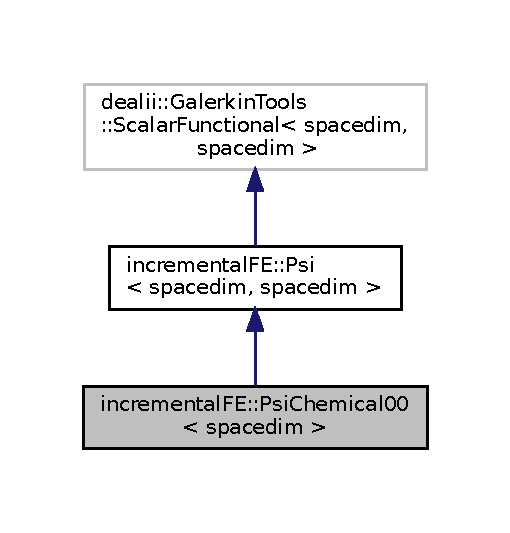
\includegraphics[width=245pt]{classincremental_f_e_1_1_psi_chemical00__inherit__graph}
\end{center}
\end{figure}


Collaboration diagram for incremental\+FE\+::Psi\+Chemical00$<$ spacedim $>$\+:\nopagebreak
\begin{figure}[H]
\begin{center}
\leavevmode
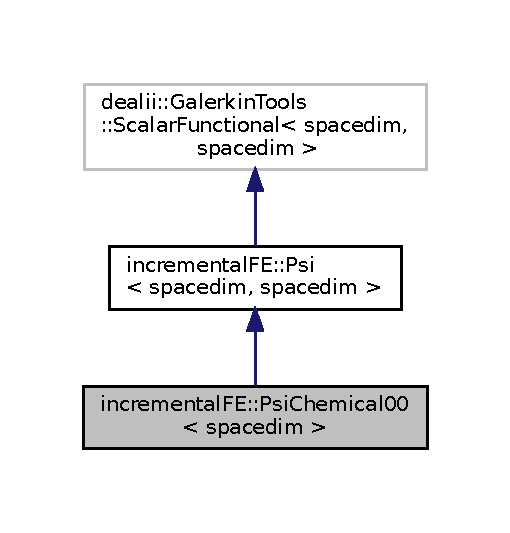
\includegraphics[width=245pt]{classincremental_f_e_1_1_psi_chemical00__coll__graph}
\end{center}
\end{figure}
\doxysubsection*{Public Member Functions}
\begin{DoxyCompactItemize}
\item 
\mbox{\hyperlink{classincremental_f_e_1_1_psi_chemical00_a2c70852c04aaa0f530c705965671f3ff}{Psi\+Chemical00}} (const std\+::vector$<$ dealii\+::\+Galerkin\+Tools\+::\+Dependent\+Field$<$ spacedim, spacedim $>$$>$ e\+\_\+omega, const std\+::set$<$ \textbf{ dealii\+::types\+::material\+\_\+id} $>$ domain\+\_\+of\+\_\+integration, const dealii\+::\+Quadrature$<$ spacedim $>$ quadrature, \mbox{\hyperlink{classincremental_f_e_1_1_global_data_incremental_f_e}{Global\+Data\+Incremental\+FE}}$<$ spacedim $>$ \&\mbox{\hyperlink{classincremental_f_e_1_1_psi_3_01spacedim_00_01spacedim_01_4_abf0a4804877fd7cc9bd1b90e52760ba9}{global\+\_\+data}}, const double \mbox{\hyperlink{classincremental_f_e_1_1_psi_chemical00_ad2500e079225b055e821ecc9e4baf3b6}{RT}}, const double \mbox{\hyperlink{classincremental_f_e_1_1_psi_chemical00_a2ad0343d949c11ca7ce23618939a623b}{c\+\_\+0}}, const double \mbox{\hyperlink{classincremental_f_e_1_1_psi_chemical00_a3c264a3e33072def54f2376ee9a0b4ea}{mu\+\_\+0}}, const double \mbox{\hyperlink{classincremental_f_e_1_1_psi_3_01spacedim_00_01spacedim_01_4_af7b8227188dbdd6ada35b9445d96c79d}{alpha}}, const double \mbox{\hyperlink{classincremental_f_e_1_1_psi_chemical00_a8016f9e379c596ca0ed60479110a3178}{eps}})
\item 
bool \mbox{\hyperlink{classincremental_f_e_1_1_psi_chemical00_a52e3a124fe8200a1cad668b12d4be439}{get\+\_\+values\+\_\+and\+\_\+derivatives}} (const \textbf{ dealii\+::\+Vector}$<$ double $>$ \&\textbf{ values}, const dealii\+::\+Point$<$ spacedim $>$ \&, double \&omega, \textbf{ dealii\+::\+Vector}$<$ double $>$ \&d\+\_\+omega, dealii\+::\+Full\+Matrix$<$ double $>$ \&d2\+\_\+omega, const std\+::tuple$<$ bool, bool, bool $>$ requested\+\_\+quantities) const
\item 
double \mbox{\hyperlink{classincremental_f_e_1_1_psi_chemical00_a0e615fbb99f3fb0826992f4eb925c947}{get\+\_\+maximum\+\_\+step}} (const \textbf{ dealii\+::\+Vector}$<$ double $>$ \&e\+\_\+omega, const std\+::vector$<$ \textbf{ dealii\+::\+Vector}$<$ double $>$$>$ \&, const \textbf{ dealii\+::\+Vector}$<$ double $>$ \&delta\+\_\+e\+\_\+omega, const \textbf{ dealii\+::\+Vector}$<$ double $>$ \&, const dealii\+::\+Point$<$ spacedim $>$ \&) const
\end{DoxyCompactItemize}
\doxysubsection*{Private Attributes}
\begin{DoxyCompactItemize}
\item 
const double \mbox{\hyperlink{classincremental_f_e_1_1_psi_chemical00_ad2500e079225b055e821ecc9e4baf3b6}{RT}}
\item 
const double \mbox{\hyperlink{classincremental_f_e_1_1_psi_chemical00_a2ad0343d949c11ca7ce23618939a623b}{c\+\_\+0}}
\item 
const double \mbox{\hyperlink{classincremental_f_e_1_1_psi_chemical00_a3c264a3e33072def54f2376ee9a0b4ea}{mu\+\_\+0}}
\item 
const double \mbox{\hyperlink{classincremental_f_e_1_1_psi_chemical00_a8016f9e379c596ca0ed60479110a3178}{eps}}
\item 
const double \mbox{\hyperlink{classincremental_f_e_1_1_psi_chemical00_a0288b7812d0350e1f38f740c010b9600}{log\+\_\+eps}}
\end{DoxyCompactItemize}
\doxysubsection*{Additional Inherited Members}


\doxysubsection{Detailed Description}
\subsubsection*{template$<$unsigned int spacedim$>$\newline
class incremental\+F\+E\+::\+Psi\+Chemical00$<$ spacedim $>$}

Class defining a domain related scalar functional with the integrand

$h^\Omega_\rho = RT c_0 h\left( \dfrac{c}{c_0} \right)$,

where

$ h(x) = \begin{cases} x [ \ln(x)-1] \quad&\mathrm{if}\quad x>\epsilon\\ \epsilon \{ \ln(\epsilon) [ \ln(x) - \ln(\epsilon) + 1] - 1\} \quad&\mathrm{else}, \end{cases} $

$R$ is the gas constant, $T$ the temperature, $c_0$ a reference species concentration, $\mu_0$ a corresponding reference value for the potential, $c$ the species concentration, and $\epsilon \ll 1$ a regularization parameter to avoid ill-\/conditioning if $c$ is too close to zero.

Ordering of quantities in \textbf{ Scalar\+Functional$<$spacedim, spacedim$>$\+::e\+\_\+omega} \+:~\newline
 \mbox{[}0\mbox{]} $c$ 

\doxysubsection{Constructor \& Destructor Documentation}
\mbox{\Hypertarget{classincremental_f_e_1_1_psi_chemical00_a2c70852c04aaa0f530c705965671f3ff}\label{classincremental_f_e_1_1_psi_chemical00_a2c70852c04aaa0f530c705965671f3ff}} 
\index{incrementalFE::PsiChemical00$<$ spacedim $>$@{incrementalFE::PsiChemical00$<$ spacedim $>$}!PsiChemical00@{PsiChemical00}}
\index{PsiChemical00@{PsiChemical00}!incrementalFE::PsiChemical00$<$ spacedim $>$@{incrementalFE::PsiChemical00$<$ spacedim $>$}}
\doxysubsubsection{\texorpdfstring{PsiChemical00()}{PsiChemical00()}}
{\footnotesize\ttfamily template$<$unsigned int spacedim$>$ \\
\mbox{\hyperlink{classincremental_f_e_1_1_psi_chemical00}{incremental\+F\+E\+::\+Psi\+Chemical00}}$<$ spacedim $>$\+::\mbox{\hyperlink{classincremental_f_e_1_1_psi_chemical00}{Psi\+Chemical00}} (\begin{DoxyParamCaption}\item[{const std\+::vector$<$ dealii\+::\+Galerkin\+Tools\+::\+Dependent\+Field$<$ spacedim, spacedim $>$$>$}]{e\+\_\+omega,  }\item[{const std\+::set$<$ \textbf{ dealii\+::types\+::material\+\_\+id} $>$}]{domain\+\_\+of\+\_\+integration,  }\item[{const dealii\+::\+Quadrature$<$ spacedim $>$}]{quadrature,  }\item[{\mbox{\hyperlink{classincremental_f_e_1_1_global_data_incremental_f_e}{Global\+Data\+Incremental\+FE}}$<$ spacedim $>$ \&}]{global\+\_\+data,  }\item[{const double}]{RT,  }\item[{const double}]{c\+\_\+0,  }\item[{const double}]{mu\+\_\+0,  }\item[{const double}]{alpha,  }\item[{const double}]{eps }\end{DoxyParamCaption})\hspace{0.3cm}{\ttfamily [inline]}}

Constructor


\begin{DoxyParams}[1]{Parameters}
\mbox{\texttt{ in}}  & {\em e\+\_\+omega} & \textbf{ Scalar\+Functional$<$spacedim, spacedim$>$\+::e\+\_\+omega}\\
\hline
\mbox{\texttt{ in}}  & {\em domain\+\_\+of\+\_\+integration} & \textbf{ Scalar\+Functional$<$spacedim, spacedim$>$\+::domain\+\_\+of\+\_\+integration}\\
\hline
\mbox{\texttt{ in}}  & {\em quadrature} & \textbf{ Scalar\+Functional$<$spacedim, spacedim$>$\+::quadrature}\\
\hline
\mbox{\texttt{ in}}  & {\em global\+\_\+data} & \mbox{\hyperlink{classincremental_f_e_1_1_psi_3_01spacedim_00_01spacedim_01_4_abf0a4804877fd7cc9bd1b90e52760ba9}{Psi$<$spacedim, spacedim$>$\+::global\+\_\+data}}\\
\hline
\mbox{\texttt{ in}}  & {\em RT} & \mbox{\hyperlink{classincremental_f_e_1_1_psi_chemical00_ad2500e079225b055e821ecc9e4baf3b6}{Psi\+Chemical00\+::\+RT}}\\
\hline
\mbox{\texttt{ in}}  & {\em c\+\_\+0} & \mbox{\hyperlink{classincremental_f_e_1_1_psi_chemical00_a2ad0343d949c11ca7ce23618939a623b}{Psi\+Chemical00\+::c\+\_\+0}}\\
\hline
\mbox{\texttt{ in}}  & {\em mu\+\_\+0} & \mbox{\hyperlink{classincremental_f_e_1_1_psi_chemical00_a3c264a3e33072def54f2376ee9a0b4ea}{Psi\+Chemical00\+::mu\+\_\+0}}\\
\hline
\mbox{\texttt{ in}}  & {\em alpha} & \mbox{\hyperlink{classincremental_f_e_1_1_psi_3_01spacedim_00_01spacedim_01_4_af7b8227188dbdd6ada35b9445d96c79d}{Psi$<$spacedim, spacedim$>$\+::alpha}}\\
\hline
\mbox{\texttt{ in}}  & {\em eps} & \mbox{\hyperlink{classincremental_f_e_1_1_psi_chemical00_a8016f9e379c596ca0ed60479110a3178}{Psi\+Chemical00\+::eps}} \\
\hline
\end{DoxyParams}


\doxysubsection{Member Function Documentation}
\mbox{\Hypertarget{classincremental_f_e_1_1_psi_chemical00_a0e615fbb99f3fb0826992f4eb925c947}\label{classincremental_f_e_1_1_psi_chemical00_a0e615fbb99f3fb0826992f4eb925c947}} 
\index{incrementalFE::PsiChemical00$<$ spacedim $>$@{incrementalFE::PsiChemical00$<$ spacedim $>$}!get\_maximum\_step@{get\_maximum\_step}}
\index{get\_maximum\_step@{get\_maximum\_step}!incrementalFE::PsiChemical00$<$ spacedim $>$@{incrementalFE::PsiChemical00$<$ spacedim $>$}}
\doxysubsubsection{\texorpdfstring{get\_maximum\_step()}{get\_maximum\_step()}}
{\footnotesize\ttfamily template$<$unsigned int spacedim$>$ \\
double \mbox{\hyperlink{classincremental_f_e_1_1_psi_chemical00}{incremental\+F\+E\+::\+Psi\+Chemical00}}$<$ spacedim $>$\+::get\+\_\+maximum\+\_\+step (\begin{DoxyParamCaption}\item[{const \textbf{ dealii\+::\+Vector}$<$ double $>$ \&}]{e\+\_\+omega,  }\item[{const std\+::vector$<$ \textbf{ dealii\+::\+Vector}$<$ double $>$$>$ \&}]{,  }\item[{const \textbf{ dealii\+::\+Vector}$<$ double $>$ \&}]{delta\+\_\+e\+\_\+omega,  }\item[{const \textbf{ dealii\+::\+Vector}$<$ double $>$ \&}]{,  }\item[{const dealii\+::\+Point$<$ spacedim $>$ \&}]{ }\end{DoxyParamCaption}) const\hspace{0.3cm}{\ttfamily [inline]}}

see \textbf{ Scalar\+Functional$<$spacedim, spacedim$>$\+::get\+\_\+maximum\+\_\+step} \mbox{\Hypertarget{classincremental_f_e_1_1_psi_chemical00_a52e3a124fe8200a1cad668b12d4be439}\label{classincremental_f_e_1_1_psi_chemical00_a52e3a124fe8200a1cad668b12d4be439}} 
\index{incrementalFE::PsiChemical00$<$ spacedim $>$@{incrementalFE::PsiChemical00$<$ spacedim $>$}!get\_values\_and\_derivatives@{get\_values\_and\_derivatives}}
\index{get\_values\_and\_derivatives@{get\_values\_and\_derivatives}!incrementalFE::PsiChemical00$<$ spacedim $>$@{incrementalFE::PsiChemical00$<$ spacedim $>$}}
\doxysubsubsection{\texorpdfstring{get\_values\_and\_derivatives()}{get\_values\_and\_derivatives()}}
{\footnotesize\ttfamily template$<$unsigned int spacedim$>$ \\
bool \mbox{\hyperlink{classincremental_f_e_1_1_psi_chemical00}{incremental\+F\+E\+::\+Psi\+Chemical00}}$<$ spacedim $>$\+::get\+\_\+values\+\_\+and\+\_\+derivatives (\begin{DoxyParamCaption}\item[{const \textbf{ dealii\+::\+Vector}$<$ double $>$ \&}]{values,  }\item[{const dealii\+::\+Point$<$ spacedim $>$ \&}]{,  }\item[{double \&}]{omega,  }\item[{\textbf{ dealii\+::\+Vector}$<$ double $>$ \&}]{d\+\_\+omega,  }\item[{dealii\+::\+Full\+Matrix$<$ double $>$ \&}]{d2\+\_\+omega,  }\item[{const std\+::tuple$<$ bool, bool, bool $>$}]{requested\+\_\+quantities }\end{DoxyParamCaption}) const\hspace{0.3cm}{\ttfamily [inline]}, {\ttfamily [virtual]}}

\begin{DoxySeeAlso}{See also}
\mbox{\hyperlink{classincremental_f_e_1_1_psi_3_01spacedim_00_01spacedim_01_4_a17f3559c196edb5487b591bb6061667e}{Psi$<$spacedim, spacedim$>$\+::get\+\_\+values\+\_\+and\+\_\+derivatives()}} 
\end{DoxySeeAlso}


Implements \mbox{\hyperlink{classincremental_f_e_1_1_psi_3_01spacedim_00_01spacedim_01_4_a17f3559c196edb5487b591bb6061667e}{incremental\+F\+E\+::\+Psi$<$ spacedim, spacedim $>$}}.



\doxysubsection{Member Data Documentation}
\mbox{\Hypertarget{classincremental_f_e_1_1_psi_chemical00_a2ad0343d949c11ca7ce23618939a623b}\label{classincremental_f_e_1_1_psi_chemical00_a2ad0343d949c11ca7ce23618939a623b}} 
\index{incrementalFE::PsiChemical00$<$ spacedim $>$@{incrementalFE::PsiChemical00$<$ spacedim $>$}!c\_0@{c\_0}}
\index{c\_0@{c\_0}!incrementalFE::PsiChemical00$<$ spacedim $>$@{incrementalFE::PsiChemical00$<$ spacedim $>$}}
\doxysubsubsection{\texorpdfstring{c\_0}{c\_0}}
{\footnotesize\ttfamily template$<$unsigned int spacedim$>$ \\
const double \mbox{\hyperlink{classincremental_f_e_1_1_psi_chemical00}{incremental\+F\+E\+::\+Psi\+Chemical00}}$<$ spacedim $>$\+::c\+\_\+0\hspace{0.3cm}{\ttfamily [private]}}

Reference concentration at which chemical potential is $RT\mu_0$ \mbox{\Hypertarget{classincremental_f_e_1_1_psi_chemical00_a8016f9e379c596ca0ed60479110a3178}\label{classincremental_f_e_1_1_psi_chemical00_a8016f9e379c596ca0ed60479110a3178}} 
\index{incrementalFE::PsiChemical00$<$ spacedim $>$@{incrementalFE::PsiChemical00$<$ spacedim $>$}!eps@{eps}}
\index{eps@{eps}!incrementalFE::PsiChemical00$<$ spacedim $>$@{incrementalFE::PsiChemical00$<$ spacedim $>$}}
\doxysubsubsection{\texorpdfstring{eps}{eps}}
{\footnotesize\ttfamily template$<$unsigned int spacedim$>$ \\
const double \mbox{\hyperlink{classincremental_f_e_1_1_psi_chemical00}{incremental\+F\+E\+::\+Psi\+Chemical00}}$<$ spacedim $>$\+::eps\hspace{0.3cm}{\ttfamily [private]}}

$\epsilon$ \mbox{\Hypertarget{classincremental_f_e_1_1_psi_chemical00_a0288b7812d0350e1f38f740c010b9600}\label{classincremental_f_e_1_1_psi_chemical00_a0288b7812d0350e1f38f740c010b9600}} 
\index{incrementalFE::PsiChemical00$<$ spacedim $>$@{incrementalFE::PsiChemical00$<$ spacedim $>$}!log\_eps@{log\_eps}}
\index{log\_eps@{log\_eps}!incrementalFE::PsiChemical00$<$ spacedim $>$@{incrementalFE::PsiChemical00$<$ spacedim $>$}}
\doxysubsubsection{\texorpdfstring{log\_eps}{log\_eps}}
{\footnotesize\ttfamily template$<$unsigned int spacedim$>$ \\
const double \mbox{\hyperlink{classincremental_f_e_1_1_psi_chemical00}{incremental\+F\+E\+::\+Psi\+Chemical00}}$<$ spacedim $>$\+::log\+\_\+eps\hspace{0.3cm}{\ttfamily [private]}}

$\ln\epsilon$ \mbox{\Hypertarget{classincremental_f_e_1_1_psi_chemical00_a3c264a3e33072def54f2376ee9a0b4ea}\label{classincremental_f_e_1_1_psi_chemical00_a3c264a3e33072def54f2376ee9a0b4ea}} 
\index{incrementalFE::PsiChemical00$<$ spacedim $>$@{incrementalFE::PsiChemical00$<$ spacedim $>$}!mu\_0@{mu\_0}}
\index{mu\_0@{mu\_0}!incrementalFE::PsiChemical00$<$ spacedim $>$@{incrementalFE::PsiChemical00$<$ spacedim $>$}}
\doxysubsubsection{\texorpdfstring{mu\_0}{mu\_0}}
{\footnotesize\ttfamily template$<$unsigned int spacedim$>$ \\
const double \mbox{\hyperlink{classincremental_f_e_1_1_psi_chemical00}{incremental\+F\+E\+::\+Psi\+Chemical00}}$<$ spacedim $>$\+::mu\+\_\+0\hspace{0.3cm}{\ttfamily [private]}}

$\mu_0$ \mbox{\Hypertarget{classincremental_f_e_1_1_psi_chemical00_ad2500e079225b055e821ecc9e4baf3b6}\label{classincremental_f_e_1_1_psi_chemical00_ad2500e079225b055e821ecc9e4baf3b6}} 
\index{incrementalFE::PsiChemical00$<$ spacedim $>$@{incrementalFE::PsiChemical00$<$ spacedim $>$}!RT@{RT}}
\index{RT@{RT}!incrementalFE::PsiChemical00$<$ spacedim $>$@{incrementalFE::PsiChemical00$<$ spacedim $>$}}
\doxysubsubsection{\texorpdfstring{RT}{RT}}
{\footnotesize\ttfamily template$<$unsigned int spacedim$>$ \\
const double \mbox{\hyperlink{classincremental_f_e_1_1_psi_chemical00}{incremental\+F\+E\+::\+Psi\+Chemical00}}$<$ spacedim $>$\+::RT\hspace{0.3cm}{\ttfamily [private]}}

gas constant times absolute temperature 

The documentation for this class was generated from the following file\+:\begin{DoxyCompactItemize}
\item 
/home/sst/code/\+Incremental\+F\+E/\+Incremental\+F\+E/include/incremental\+\_\+fe/scalar\+\_\+functionals/\mbox{\hyperlink{psi__lib_8h}{psi\+\_\+lib.\+h}}\end{DoxyCompactItemize}

\hypertarget{classincremental_f_e_1_1_psi_chemical01}{}\section{incremental\+FE\+:\+:Psi\+Chemical01$<$ spacedim $>$ Class Template Reference}
\label{classincremental_f_e_1_1_psi_chemical01}\index{incremental\+F\+E\+::\+Psi\+Chemical01$<$ spacedim $>$@{incremental\+F\+E\+::\+Psi\+Chemical01$<$ spacedim $>$}}


{\ttfamily \#include $<$psi\+\_\+lib.\+h$>$}



Inheritance diagram for incremental\+FE\+:\+:Psi\+Chemical01$<$ spacedim $>$\+:\nopagebreak
\begin{figure}[H]
\begin{center}
\leavevmode
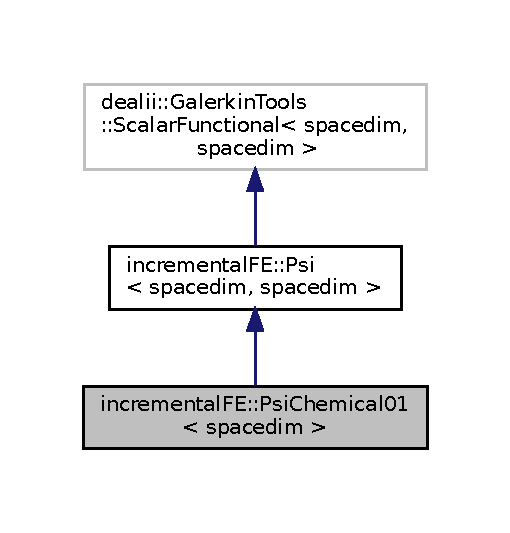
\includegraphics[width=232pt]{classincremental_f_e_1_1_psi_chemical01__inherit__graph}
\end{center}
\end{figure}


Collaboration diagram for incremental\+FE\+:\+:Psi\+Chemical01$<$ spacedim $>$\+:\nopagebreak
\begin{figure}[H]
\begin{center}
\leavevmode
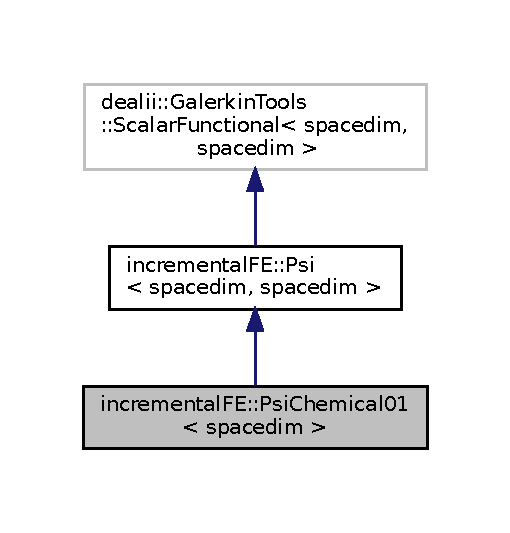
\includegraphics[width=232pt]{classincremental_f_e_1_1_psi_chemical01__coll__graph}
\end{center}
\end{figure}
\subsection*{Public Member Functions}
\begin{DoxyCompactItemize}
\item 
\hyperlink{classincremental_f_e_1_1_psi_chemical01_a5a434806969a774863983047152ecf71}{Psi\+Chemical01} (const std\+::vector$<$ dealii\+::\+Galerkin\+Tools\+::\+Dependent\+Field$<$ spacedim, spacedim $>$$>$ e\+\_\+omega, const std\+::set$<$ {\bf dealii\+::types\+::material\+\_\+id} $>$ domain\+\_\+of\+\_\+integration, const dealii\+::\+Quadrature$<$ spacedim $>$ quadrature, \hyperlink{classincremental_f_e_1_1_global_data_incremental_f_e}{Global\+Data\+Incremental\+FE}$<$ spacedim $>$ \&\hyperlink{classincremental_f_e_1_1_psi_3_01spacedim_00_01spacedim_01_4_abf0a4804877fd7cc9bd1b90e52760ba9}{global\+\_\+data}, const double \hyperlink{classincremental_f_e_1_1_psi_chemical01_a8af1cff2abb682cf14582de4a9a1bc85}{a}, const double \hyperlink{classincremental_f_e_1_1_psi_chemical01_ad445df6815f30a51be2b2443b0477871}{b}, const double \hyperlink{classincremental_f_e_1_1_psi_3_01spacedim_00_01spacedim_01_4_af7b8227188dbdd6ada35b9445d96c79d}{alpha})
\item 
bool \hyperlink{classincremental_f_e_1_1_psi_chemical01_a5455473224a9770a1f65d6418f523a39}{get\+\_\+values\+\_\+and\+\_\+derivatives} (const {\bf dealii\+::\+Vector}$<$ double $>$ \&{\bf values}, const dealii\+::\+Point$<$ spacedim $>$ \&, double \&omega, {\bf dealii\+::\+Vector}$<$ double $>$ \&d\+\_\+omega, dealii\+::\+Full\+Matrix$<$ double $>$ \&d2\+\_\+omega, const std\+::tuple$<$ bool, bool, bool $>$ requested\+\_\+quantities) const 
\end{DoxyCompactItemize}
\subsection*{Private Attributes}
\begin{DoxyCompactItemize}
\item 
const double \hyperlink{classincremental_f_e_1_1_psi_chemical01_a8af1cff2abb682cf14582de4a9a1bc85}{a}
\item 
const double \hyperlink{classincremental_f_e_1_1_psi_chemical01_ad445df6815f30a51be2b2443b0477871}{b}
\end{DoxyCompactItemize}


\subsection{Detailed Description}
\subsubsection*{template$<$unsigned int spacedim$>$\\*
class incremental\+F\+E\+::\+Psi\+Chemical01$<$ spacedim $>$}

Class defining a domain related scalar functional with the integrand

$h^\Omega_\rho = \dfrac{a}{2} (c-b)^2$,

where $a$ and $b$ are material parameters, and $c$ the species concentration.

Ordering of quantities in {\bf Scalar\+Functional$<$spacedim, spacedim$>$\+::e\+\_\+omega} \+:~\newline
 \mbox{[}0\mbox{]} $c$ 

\subsection{Constructor \& Destructor Documentation}
\index{incremental\+F\+E\+::\+Psi\+Chemical01@{incremental\+F\+E\+::\+Psi\+Chemical01}!Psi\+Chemical01@{Psi\+Chemical01}}
\index{Psi\+Chemical01@{Psi\+Chemical01}!incremental\+F\+E\+::\+Psi\+Chemical01@{incremental\+F\+E\+::\+Psi\+Chemical01}}
\subsubsection[{\texorpdfstring{Psi\+Chemical01(const std\+::vector$<$ dealii\+::\+Galerkin\+Tools\+::\+Dependent\+Field$<$ spacedim, spacedim $>$$>$ e\+\_\+omega, const std\+::set$<$ dealii\+::types\+::material\+\_\+id $>$ domain\+\_\+of\+\_\+integration, const dealii\+::\+Quadrature$<$ spacedim $>$ quadrature, Global\+Data\+Incremental\+F\+E$<$ spacedim $>$ \&global\+\_\+data, const double a, const double b, const double alpha)}{PsiChemical01(const std::vector< dealii::GalerkinTools::DependentField< spacedim, spacedim >> e_omega, const std::set< dealii::types::material_id > domain_of_integration, const dealii::Quadrature< spacedim > quadrature, GlobalDataIncrementalFE< spacedim > &global_data, const double a, const double b, const double alpha)}}]{\setlength{\rightskip}{0pt plus 5cm}template$<$unsigned int spacedim$>$ {\bf incremental\+F\+E\+::\+Psi\+Chemical01}$<$ spacedim $>$\+::{\bf Psi\+Chemical01} (
\begin{DoxyParamCaption}
\item[{const std\+::vector$<$ dealii\+::\+Galerkin\+Tools\+::\+Dependent\+Field$<$ spacedim, spacedim $>$$>$}]{e\+\_\+omega, }
\item[{const std\+::set$<$ {\bf dealii\+::types\+::material\+\_\+id} $>$}]{domain\+\_\+of\+\_\+integration, }
\item[{const dealii\+::\+Quadrature$<$ spacedim $>$}]{quadrature, }
\item[{{\bf Global\+Data\+Incremental\+FE}$<$ spacedim $>$ \&}]{global\+\_\+data, }
\item[{const double}]{a, }
\item[{const double}]{b, }
\item[{const double}]{alpha}
\end{DoxyParamCaption}
)\hspace{0.3cm}{\ttfamily [inline]}}\hypertarget{classincremental_f_e_1_1_psi_chemical01_a5a434806969a774863983047152ecf71}{}\label{classincremental_f_e_1_1_psi_chemical01_a5a434806969a774863983047152ecf71}
Constructor


\begin{DoxyParams}[1]{Parameters}
\mbox{\tt in}  & {\em e\+\_\+omega} & {\bf Scalar\+Functional$<$spacedim, spacedim$>$\+::e\+\_\+omega}\\
\hline
\mbox{\tt in}  & {\em domain\+\_\+of\+\_\+integration} & {\bf Scalar\+Functional$<$spacedim, spacedim$>$\+::domain\+\_\+of\+\_\+integration}\\
\hline
\mbox{\tt in}  & {\em quadrature} & {\bf Scalar\+Functional$<$spacedim, spacedim$>$\+::quadrature}\\
\hline
\mbox{\tt in}  & {\em global\+\_\+data} & \hyperlink{classincremental_f_e_1_1_psi_3_01spacedim_00_01spacedim_01_4_abf0a4804877fd7cc9bd1b90e52760ba9}{Psi$<$spacedim, spacedim$>$\+::global\+\_\+data}\\
\hline
\mbox{\tt in}  & {\em a} & \hyperlink{classincremental_f_e_1_1_psi_chemical01_a8af1cff2abb682cf14582de4a9a1bc85}{Psi\+Chemical01\+::a}\\
\hline
\mbox{\tt in}  & {\em b} & \hyperlink{classincremental_f_e_1_1_psi_chemical01_ad445df6815f30a51be2b2443b0477871}{Psi\+Chemical01\+::b}\\
\hline
\mbox{\tt in}  & {\em alpha} & \hyperlink{classincremental_f_e_1_1_psi_3_01spacedim_00_01spacedim_01_4_af7b8227188dbdd6ada35b9445d96c79d}{Psi$<$spacedim, spacedim$>$\+::alpha} \\
\hline
\end{DoxyParams}


\subsection{Member Function Documentation}
\index{incremental\+F\+E\+::\+Psi\+Chemical01@{incremental\+F\+E\+::\+Psi\+Chemical01}!get\+\_\+values\+\_\+and\+\_\+derivatives@{get\+\_\+values\+\_\+and\+\_\+derivatives}}
\index{get\+\_\+values\+\_\+and\+\_\+derivatives@{get\+\_\+values\+\_\+and\+\_\+derivatives}!incremental\+F\+E\+::\+Psi\+Chemical01@{incremental\+F\+E\+::\+Psi\+Chemical01}}
\subsubsection[{\texorpdfstring{get\+\_\+values\+\_\+and\+\_\+derivatives(const dealii\+::\+Vector$<$ double $>$ \&values, const dealii\+::\+Point$<$ spacedim $>$ \&, double \&omega, dealii\+::\+Vector$<$ double $>$ \&d\+\_\+omega, dealii\+::\+Full\+Matrix$<$ double $>$ \&d2\+\_\+omega, const std\+::tuple$<$ bool, bool, bool $>$ requested\+\_\+quantities) const }{get_values_and_derivatives(const dealii::Vector< double > &values, const dealii::Point< spacedim > &, double &omega, dealii::Vector< double > &d_omega, dealii::FullMatrix< double > &d2_omega, const std::tuple< bool, bool, bool > requested_quantities) const }}]{\setlength{\rightskip}{0pt plus 5cm}template$<$unsigned int spacedim$>$ bool {\bf incremental\+F\+E\+::\+Psi\+Chemical01}$<$ spacedim $>$\+::get\+\_\+values\+\_\+and\+\_\+derivatives (
\begin{DoxyParamCaption}
\item[{const {\bf dealii\+::\+Vector}$<$ double $>$ \&}]{values, }
\item[{const dealii\+::\+Point$<$ spacedim $>$ \&}]{, }
\item[{double \&}]{omega, }
\item[{{\bf dealii\+::\+Vector}$<$ double $>$ \&}]{d\+\_\+omega, }
\item[{dealii\+::\+Full\+Matrix$<$ double $>$ \&}]{d2\+\_\+omega, }
\item[{const std\+::tuple$<$ bool, bool, bool $>$}]{requested\+\_\+quantities}
\end{DoxyParamCaption}
) const\hspace{0.3cm}{\ttfamily [inline]}, {\ttfamily [virtual]}}\hypertarget{classincremental_f_e_1_1_psi_chemical01_a5455473224a9770a1f65d6418f523a39}{}\label{classincremental_f_e_1_1_psi_chemical01_a5455473224a9770a1f65d6418f523a39}
\begin{DoxySeeAlso}{See also}
\hyperlink{classincremental_f_e_1_1_psi_3_01spacedim_00_01spacedim_01_4_a17f3559c196edb5487b591bb6061667e}{Psi$<$spacedim, spacedim$>$\+::get\+\_\+values\+\_\+and\+\_\+derivatives()} 
\end{DoxySeeAlso}


Implements \hyperlink{classincremental_f_e_1_1_psi_3_01spacedim_00_01spacedim_01_4_a17f3559c196edb5487b591bb6061667e}{incremental\+F\+E\+::\+Psi$<$ spacedim, spacedim $>$}.



\subsection{Member Data Documentation}
\index{incremental\+F\+E\+::\+Psi\+Chemical01@{incremental\+F\+E\+::\+Psi\+Chemical01}!a@{a}}
\index{a@{a}!incremental\+F\+E\+::\+Psi\+Chemical01@{incremental\+F\+E\+::\+Psi\+Chemical01}}
\subsubsection[{\texorpdfstring{a}{a}}]{\setlength{\rightskip}{0pt plus 5cm}template$<$unsigned int spacedim$>$ const double {\bf incremental\+F\+E\+::\+Psi\+Chemical01}$<$ spacedim $>$\+::a\hspace{0.3cm}{\ttfamily [private]}}\hypertarget{classincremental_f_e_1_1_psi_chemical01_a8af1cff2abb682cf14582de4a9a1bc85}{}\label{classincremental_f_e_1_1_psi_chemical01_a8af1cff2abb682cf14582de4a9a1bc85}
$a$ \index{incremental\+F\+E\+::\+Psi\+Chemical01@{incremental\+F\+E\+::\+Psi\+Chemical01}!b@{b}}
\index{b@{b}!incremental\+F\+E\+::\+Psi\+Chemical01@{incremental\+F\+E\+::\+Psi\+Chemical01}}
\subsubsection[{\texorpdfstring{b}{b}}]{\setlength{\rightskip}{0pt plus 5cm}template$<$unsigned int spacedim$>$ const double {\bf incremental\+F\+E\+::\+Psi\+Chemical01}$<$ spacedim $>$\+::b\hspace{0.3cm}{\ttfamily [private]}}\hypertarget{classincremental_f_e_1_1_psi_chemical01_ad445df6815f30a51be2b2443b0477871}{}\label{classincremental_f_e_1_1_psi_chemical01_ad445df6815f30a51be2b2443b0477871}
$b$ 

The documentation for this class was generated from the following file\+:\begin{DoxyCompactItemize}
\item 
/home/sst/code/\+Incremental\+F\+E/\+Incremental\+F\+E/include/incremental\+\_\+fe/scalar\+\_\+functionals/\hyperlink{psi__lib_8h}{psi\+\_\+lib.\+h}\end{DoxyCompactItemize}

\hypertarget{classincremental_f_e_1_1_psi_chemical02}{}\doxysection{incremental\+FE\+::Psi\+Chemical02$<$ spacedim $>$ Class Template Reference}
\label{classincremental_f_e_1_1_psi_chemical02}\index{incrementalFE::PsiChemical02$<$ spacedim $>$@{incrementalFE::PsiChemical02$<$ spacedim $>$}}


{\ttfamily \#include $<$psi\+\_\+lib.\+h$>$}



Inheritance diagram for incremental\+FE\+::Psi\+Chemical02$<$ spacedim $>$\+:\nopagebreak
\begin{figure}[H]
\begin{center}
\leavevmode
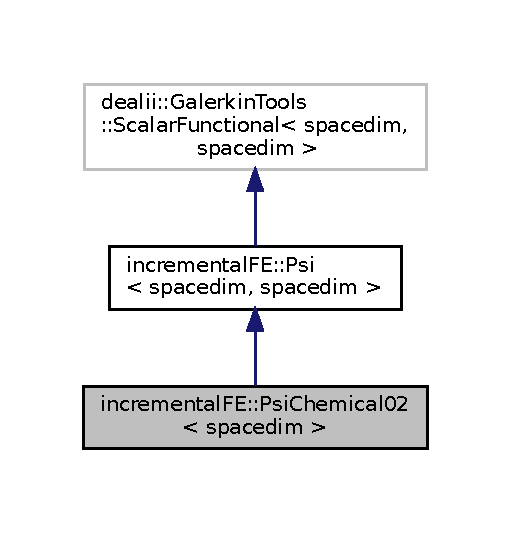
\includegraphics[width=245pt]{classincremental_f_e_1_1_psi_chemical02__inherit__graph}
\end{center}
\end{figure}


Collaboration diagram for incremental\+FE\+::Psi\+Chemical02$<$ spacedim $>$\+:\nopagebreak
\begin{figure}[H]
\begin{center}
\leavevmode
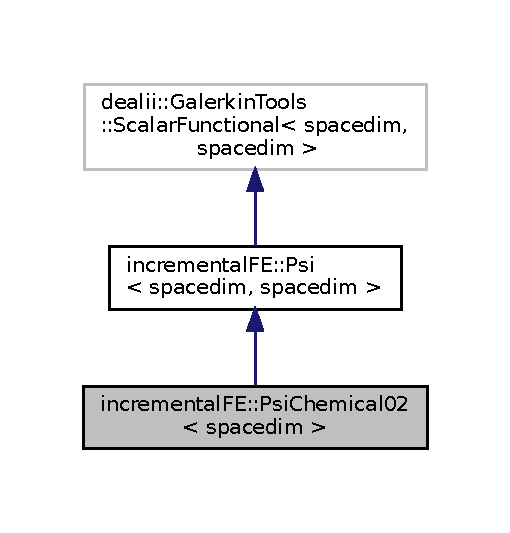
\includegraphics[width=245pt]{classincremental_f_e_1_1_psi_chemical02__coll__graph}
\end{center}
\end{figure}
\doxysubsection*{Public Member Functions}
\begin{DoxyCompactItemize}
\item 
\mbox{\hyperlink{classincremental_f_e_1_1_psi_chemical02_a82b105addb1311b165edfcdfbd4d0699}{Psi\+Chemical02}} (const std\+::vector$<$ dealii\+::\+Galerkin\+Tools\+::\+Dependent\+Field$<$ spacedim, spacedim $>$$>$ e\+\_\+omega, const std\+::set$<$ \textbf{ dealii\+::types\+::material\+\_\+id} $>$ domain\+\_\+of\+\_\+integration, const dealii\+::\+Quadrature$<$ spacedim $>$ quadrature, \mbox{\hyperlink{classincremental_f_e_1_1_global_data_incremental_f_e}{Global\+Data\+Incremental\+FE}}$<$ spacedim $>$ \&\mbox{\hyperlink{classincremental_f_e_1_1_psi_3_01spacedim_00_01spacedim_01_4_abf0a4804877fd7cc9bd1b90e52760ba9}{global\+\_\+data}}, const double \mbox{\hyperlink{classincremental_f_e_1_1_psi_chemical02_a4b93e968af97d8497a53be13980ef22e}{RT}}, const double \mbox{\hyperlink{classincremental_f_e_1_1_psi_chemical02_a70426dc3fa6acda53984c2e178ad92c5}{mu\+\_\+0}}, const double \mbox{\hyperlink{classincremental_f_e_1_1_psi_3_01spacedim_00_01spacedim_01_4_aaeb0d41ffa60afde6010e30270d47801}{alpha}}, const double \mbox{\hyperlink{classincremental_f_e_1_1_psi_chemical02_a1062004f111d9b425c16e3e3c1c4ce20}{eps}}=0.\+0, const double \mbox{\hyperlink{classincremental_f_e_1_1_psi_chemical02_aa2b9c1f2f65985cd003d9e33a5e54875}{c\+\_\+0\+\_\+c\+\_\+f\+\_\+0}}=1.\+0)
\item 
bool \mbox{\hyperlink{classincremental_f_e_1_1_psi_chemical02_addfb3bb4446157cfe28064f34f67429d}{get\+\_\+values\+\_\+and\+\_\+derivatives}} (const \textbf{ dealii\+::\+Vector}$<$ double $>$ \&\textbf{ values}, const dealii\+::\+Point$<$ spacedim $>$ \&, double \&omega, \textbf{ dealii\+::\+Vector}$<$ double $>$ \&d\+\_\+omega, dealii\+::\+Full\+Matrix$<$ double $>$ \&d2\+\_\+omega, const std\+::tuple$<$ bool, bool, bool $>$ requested\+\_\+quantities) const
\item 
double \mbox{\hyperlink{classincremental_f_e_1_1_psi_chemical02_aaef5025406632ddf15caba21e3b87689}{get\+\_\+maximum\+\_\+step}} (const \textbf{ dealii\+::\+Vector}$<$ double $>$ \&e\+\_\+omega, const std\+::vector$<$ \textbf{ dealii\+::\+Vector}$<$ double $>$$>$ \&, const \textbf{ dealii\+::\+Vector}$<$ double $>$ \&delta\+\_\+e\+\_\+omega, const \textbf{ dealii\+::\+Vector}$<$ double $>$ \&, const dealii\+::\+Point$<$ spacedim $>$ \&) const
\end{DoxyCompactItemize}
\doxysubsection*{Private Attributes}
\begin{DoxyCompactItemize}
\item 
const double \mbox{\hyperlink{classincremental_f_e_1_1_psi_chemical02_a4b93e968af97d8497a53be13980ef22e}{RT}}
\item 
const double \mbox{\hyperlink{classincremental_f_e_1_1_psi_chemical02_a70426dc3fa6acda53984c2e178ad92c5}{mu\+\_\+0}}
\item 
const double \mbox{\hyperlink{classincremental_f_e_1_1_psi_chemical02_a1062004f111d9b425c16e3e3c1c4ce20}{eps}}
\item 
const double \mbox{\hyperlink{classincremental_f_e_1_1_psi_chemical02_aa2b9c1f2f65985cd003d9e33a5e54875}{c\+\_\+0\+\_\+c\+\_\+f\+\_\+0}}
\item 
const double \mbox{\hyperlink{classincremental_f_e_1_1_psi_chemical02_a37ddfb3a86936177344fafd95f8eb377}{log\+\_\+eps}}
\item 
const double \mbox{\hyperlink{classincremental_f_e_1_1_psi_chemical02_a35ebf4f4790fd12b1660146f2714704a}{log\+\_\+c\+\_\+0\+\_\+c\+\_\+f\+\_\+0}}
\end{DoxyCompactItemize}
\doxysubsection*{Additional Inherited Members}


\doxysubsection{Detailed Description}
\subsubsection*{template$<$unsigned int spacedim$>$\newline
class incremental\+F\+E\+::\+Psi\+Chemical02$<$ spacedim $>$}

Class defining chemical potential of charged species moving in fluid

$h^\Omega_\rho = \mu_0 c + RT c \left( \ln\dfrac{c}{c^\mathrm{f}} - 1 \right)$,

where $\mu_0$ is a reference chemical potential, $R$ the gas constant, $T$ the temperature, $c$ the species concentration, and $c^\mathrm{f}$ the fluid concentration.

In order to circumvent numerical problems for low species concentrations, the scalar functional may be regularized according to

$h^\Omega_\rho = RT c^\mathrm{f} \dfrac{c_0}{c^\mathrm{f}_0} h\left( \dfrac{c c^\mathrm{f}_0}{c^\mathrm{f} c_0} \right)$,

where

$ h(x) = \begin{cases} x [ \ln(x)-1] \quad&\mathrm{if}\quad x>\epsilon\\ \epsilon \{ \ln(\epsilon) [ \ln(x) - \ln(\epsilon) + 1] - 1\} \quad&\mathrm{else}, \end{cases} $,

with $\epsilon \ll 1$ being a regularization parameter.

Ordering of quantities in \textbf{ Scalar\+Functional$<$spacedim, spacedim$>$\+::e\+\_\+omega} \+:~\newline
 \mbox{[}0\mbox{]} $c$~\newline
 \mbox{[}1\mbox{]} $c^\mathrm{f}$ 

\doxysubsection{Constructor \& Destructor Documentation}
\mbox{\Hypertarget{classincremental_f_e_1_1_psi_chemical02_a82b105addb1311b165edfcdfbd4d0699}\label{classincremental_f_e_1_1_psi_chemical02_a82b105addb1311b165edfcdfbd4d0699}} 
\index{incrementalFE::PsiChemical02$<$ spacedim $>$@{incrementalFE::PsiChemical02$<$ spacedim $>$}!PsiChemical02@{PsiChemical02}}
\index{PsiChemical02@{PsiChemical02}!incrementalFE::PsiChemical02$<$ spacedim $>$@{incrementalFE::PsiChemical02$<$ spacedim $>$}}
\doxysubsubsection{\texorpdfstring{PsiChemical02()}{PsiChemical02()}}
{\footnotesize\ttfamily template$<$unsigned int spacedim$>$ \\
\mbox{\hyperlink{classincremental_f_e_1_1_psi_chemical02}{incremental\+F\+E\+::\+Psi\+Chemical02}}$<$ spacedim $>$\+::\mbox{\hyperlink{classincremental_f_e_1_1_psi_chemical02}{Psi\+Chemical02}} (\begin{DoxyParamCaption}\item[{const std\+::vector$<$ dealii\+::\+Galerkin\+Tools\+::\+Dependent\+Field$<$ spacedim, spacedim $>$$>$}]{e\+\_\+omega,  }\item[{const std\+::set$<$ \textbf{ dealii\+::types\+::material\+\_\+id} $>$}]{domain\+\_\+of\+\_\+integration,  }\item[{const dealii\+::\+Quadrature$<$ spacedim $>$}]{quadrature,  }\item[{\mbox{\hyperlink{classincremental_f_e_1_1_global_data_incremental_f_e}{Global\+Data\+Incremental\+FE}}$<$ spacedim $>$ \&}]{global\+\_\+data,  }\item[{const double}]{RT,  }\item[{const double}]{mu\+\_\+0,  }\item[{const double}]{alpha,  }\item[{const double}]{eps = {\ttfamily 0.0},  }\item[{const double}]{c\+\_\+0\+\_\+c\+\_\+f\+\_\+0 = {\ttfamily 1.0} }\end{DoxyParamCaption})\hspace{0.3cm}{\ttfamily [inline]}}

Constructor


\begin{DoxyParams}[1]{Parameters}
\mbox{\texttt{ in}}  & {\em e\+\_\+omega} & \textbf{ Scalar\+Functional$<$spacedim, spacedim$>$\+::e\+\_\+omega}\\
\hline
\mbox{\texttt{ in}}  & {\em domain\+\_\+of\+\_\+integration} & \textbf{ Scalar\+Functional$<$spacedim, spacedim$>$\+::domain\+\_\+of\+\_\+integration}\\
\hline
\mbox{\texttt{ in}}  & {\em quadrature} & \textbf{ Scalar\+Functional$<$spacedim, spacedim$>$\+::quadrature}\\
\hline
\mbox{\texttt{ in}}  & {\em global\+\_\+data} & \mbox{\hyperlink{classincremental_f_e_1_1_psi_3_01spacedim_00_01spacedim_01_4_abf0a4804877fd7cc9bd1b90e52760ba9}{Psi$<$spacedim, spacedim$>$\+::global\+\_\+data}}\\
\hline
\mbox{\texttt{ in}}  & {\em RT} & \mbox{\hyperlink{classincremental_f_e_1_1_psi_chemical02_a4b93e968af97d8497a53be13980ef22e}{Psi\+Chemical02\+::\+RT}}\\
\hline
\mbox{\texttt{ in}}  & {\em mu\+\_\+0} & \mbox{\hyperlink{classincremental_f_e_1_1_psi_chemical02_a70426dc3fa6acda53984c2e178ad92c5}{Psi\+Chemical02\+::mu\+\_\+0}}\\
\hline
\mbox{\texttt{ in}}  & {\em alpha} & \mbox{\hyperlink{classincremental_f_e_1_1_psi_3_01spacedim_00_01spacedim_01_4_aaeb0d41ffa60afde6010e30270d47801}{Psi$<$spacedim, spacedim$>$\+::alpha}}\\
\hline
\mbox{\texttt{ in}}  & {\em eps} & \mbox{\hyperlink{classincremental_f_e_1_1_psi_chemical02_a1062004f111d9b425c16e3e3c1c4ce20}{Psi\+Chemical02\+::eps}}\\
\hline
\mbox{\texttt{ in}}  & {\em c\+\_\+0\+\_\+c\+\_\+f\+\_\+0} & Psi\+Chemical02\+::c\+\_\+f\+\_\+c\+\_\+f\+\_\+0 \\
\hline
\end{DoxyParams}


\doxysubsection{Member Function Documentation}
\mbox{\Hypertarget{classincremental_f_e_1_1_psi_chemical02_aaef5025406632ddf15caba21e3b87689}\label{classincremental_f_e_1_1_psi_chemical02_aaef5025406632ddf15caba21e3b87689}} 
\index{incrementalFE::PsiChemical02$<$ spacedim $>$@{incrementalFE::PsiChemical02$<$ spacedim $>$}!get\_maximum\_step@{get\_maximum\_step}}
\index{get\_maximum\_step@{get\_maximum\_step}!incrementalFE::PsiChemical02$<$ spacedim $>$@{incrementalFE::PsiChemical02$<$ spacedim $>$}}
\doxysubsubsection{\texorpdfstring{get\_maximum\_step()}{get\_maximum\_step()}}
{\footnotesize\ttfamily template$<$unsigned int spacedim$>$ \\
double \mbox{\hyperlink{classincremental_f_e_1_1_psi_chemical02}{incremental\+F\+E\+::\+Psi\+Chemical02}}$<$ spacedim $>$\+::get\+\_\+maximum\+\_\+step (\begin{DoxyParamCaption}\item[{const \textbf{ dealii\+::\+Vector}$<$ double $>$ \&}]{e\+\_\+omega,  }\item[{const std\+::vector$<$ \textbf{ dealii\+::\+Vector}$<$ double $>$$>$ \&}]{,  }\item[{const \textbf{ dealii\+::\+Vector}$<$ double $>$ \&}]{delta\+\_\+e\+\_\+omega,  }\item[{const \textbf{ dealii\+::\+Vector}$<$ double $>$ \&}]{,  }\item[{const dealii\+::\+Point$<$ spacedim $>$ \&}]{ }\end{DoxyParamCaption}) const\hspace{0.3cm}{\ttfamily [inline]}}

see \textbf{ Scalar\+Functional$<$spacedim, spacedim$>$\+::get\+\_\+maximum\+\_\+step} \mbox{\Hypertarget{classincremental_f_e_1_1_psi_chemical02_addfb3bb4446157cfe28064f34f67429d}\label{classincremental_f_e_1_1_psi_chemical02_addfb3bb4446157cfe28064f34f67429d}} 
\index{incrementalFE::PsiChemical02$<$ spacedim $>$@{incrementalFE::PsiChemical02$<$ spacedim $>$}!get\_values\_and\_derivatives@{get\_values\_and\_derivatives}}
\index{get\_values\_and\_derivatives@{get\_values\_and\_derivatives}!incrementalFE::PsiChemical02$<$ spacedim $>$@{incrementalFE::PsiChemical02$<$ spacedim $>$}}
\doxysubsubsection{\texorpdfstring{get\_values\_and\_derivatives()}{get\_values\_and\_derivatives()}}
{\footnotesize\ttfamily template$<$unsigned int spacedim$>$ \\
bool \mbox{\hyperlink{classincremental_f_e_1_1_psi_chemical02}{incremental\+F\+E\+::\+Psi\+Chemical02}}$<$ spacedim $>$\+::get\+\_\+values\+\_\+and\+\_\+derivatives (\begin{DoxyParamCaption}\item[{const \textbf{ dealii\+::\+Vector}$<$ double $>$ \&}]{values,  }\item[{const dealii\+::\+Point$<$ spacedim $>$ \&}]{,  }\item[{double \&}]{omega,  }\item[{\textbf{ dealii\+::\+Vector}$<$ double $>$ \&}]{d\+\_\+omega,  }\item[{dealii\+::\+Full\+Matrix$<$ double $>$ \&}]{d2\+\_\+omega,  }\item[{const std\+::tuple$<$ bool, bool, bool $>$}]{requested\+\_\+quantities }\end{DoxyParamCaption}) const\hspace{0.3cm}{\ttfamily [inline]}, {\ttfamily [virtual]}}

\begin{DoxySeeAlso}{See also}
\mbox{\hyperlink{classincremental_f_e_1_1_psi_3_01spacedim_00_01spacedim_01_4_a17f3559c196edb5487b591bb6061667e}{Psi$<$spacedim, spacedim$>$\+::get\+\_\+values\+\_\+and\+\_\+derivatives()}} 
\end{DoxySeeAlso}


Implements \mbox{\hyperlink{classincremental_f_e_1_1_psi_3_01spacedim_00_01spacedim_01_4_a17f3559c196edb5487b591bb6061667e}{incremental\+F\+E\+::\+Psi$<$ spacedim, spacedim $>$}}.



\doxysubsection{Member Data Documentation}
\mbox{\Hypertarget{classincremental_f_e_1_1_psi_chemical02_aa2b9c1f2f65985cd003d9e33a5e54875}\label{classincremental_f_e_1_1_psi_chemical02_aa2b9c1f2f65985cd003d9e33a5e54875}} 
\index{incrementalFE::PsiChemical02$<$ spacedim $>$@{incrementalFE::PsiChemical02$<$ spacedim $>$}!c\_0\_c\_f\_0@{c\_0\_c\_f\_0}}
\index{c\_0\_c\_f\_0@{c\_0\_c\_f\_0}!incrementalFE::PsiChemical02$<$ spacedim $>$@{incrementalFE::PsiChemical02$<$ spacedim $>$}}
\doxysubsubsection{\texorpdfstring{c\_0\_c\_f\_0}{c\_0\_c\_f\_0}}
{\footnotesize\ttfamily template$<$unsigned int spacedim$>$ \\
const double \mbox{\hyperlink{classincremental_f_e_1_1_psi_chemical02}{incremental\+F\+E\+::\+Psi\+Chemical02}}$<$ spacedim $>$\+::c\+\_\+0\+\_\+c\+\_\+f\+\_\+0\hspace{0.3cm}{\ttfamily [private]}}

$c_0 / c^\mathrm{f}_0$ \mbox{\Hypertarget{classincremental_f_e_1_1_psi_chemical02_a1062004f111d9b425c16e3e3c1c4ce20}\label{classincremental_f_e_1_1_psi_chemical02_a1062004f111d9b425c16e3e3c1c4ce20}} 
\index{incrementalFE::PsiChemical02$<$ spacedim $>$@{incrementalFE::PsiChemical02$<$ spacedim $>$}!eps@{eps}}
\index{eps@{eps}!incrementalFE::PsiChemical02$<$ spacedim $>$@{incrementalFE::PsiChemical02$<$ spacedim $>$}}
\doxysubsubsection{\texorpdfstring{eps}{eps}}
{\footnotesize\ttfamily template$<$unsigned int spacedim$>$ \\
const double \mbox{\hyperlink{classincremental_f_e_1_1_psi_chemical02}{incremental\+F\+E\+::\+Psi\+Chemical02}}$<$ spacedim $>$\+::eps\hspace{0.3cm}{\ttfamily [private]}}

$\epsilon$ \mbox{\Hypertarget{classincremental_f_e_1_1_psi_chemical02_a35ebf4f4790fd12b1660146f2714704a}\label{classincremental_f_e_1_1_psi_chemical02_a35ebf4f4790fd12b1660146f2714704a}} 
\index{incrementalFE::PsiChemical02$<$ spacedim $>$@{incrementalFE::PsiChemical02$<$ spacedim $>$}!log\_c\_0\_c\_f\_0@{log\_c\_0\_c\_f\_0}}
\index{log\_c\_0\_c\_f\_0@{log\_c\_0\_c\_f\_0}!incrementalFE::PsiChemical02$<$ spacedim $>$@{incrementalFE::PsiChemical02$<$ spacedim $>$}}
\doxysubsubsection{\texorpdfstring{log\_c\_0\_c\_f\_0}{log\_c\_0\_c\_f\_0}}
{\footnotesize\ttfamily template$<$unsigned int spacedim$>$ \\
const double \mbox{\hyperlink{classincremental_f_e_1_1_psi_chemical02}{incremental\+F\+E\+::\+Psi\+Chemical02}}$<$ spacedim $>$\+::log\+\_\+c\+\_\+0\+\_\+c\+\_\+f\+\_\+0\hspace{0.3cm}{\ttfamily [private]}}

$\ln(c_0 / c^\mathrm{f}_0)$ \mbox{\Hypertarget{classincremental_f_e_1_1_psi_chemical02_a37ddfb3a86936177344fafd95f8eb377}\label{classincremental_f_e_1_1_psi_chemical02_a37ddfb3a86936177344fafd95f8eb377}} 
\index{incrementalFE::PsiChemical02$<$ spacedim $>$@{incrementalFE::PsiChemical02$<$ spacedim $>$}!log\_eps@{log\_eps}}
\index{log\_eps@{log\_eps}!incrementalFE::PsiChemical02$<$ spacedim $>$@{incrementalFE::PsiChemical02$<$ spacedim $>$}}
\doxysubsubsection{\texorpdfstring{log\_eps}{log\_eps}}
{\footnotesize\ttfamily template$<$unsigned int spacedim$>$ \\
const double \mbox{\hyperlink{classincremental_f_e_1_1_psi_chemical02}{incremental\+F\+E\+::\+Psi\+Chemical02}}$<$ spacedim $>$\+::log\+\_\+eps\hspace{0.3cm}{\ttfamily [private]}}

$\ln(\epsilon)$ \mbox{\Hypertarget{classincremental_f_e_1_1_psi_chemical02_a70426dc3fa6acda53984c2e178ad92c5}\label{classincremental_f_e_1_1_psi_chemical02_a70426dc3fa6acda53984c2e178ad92c5}} 
\index{incrementalFE::PsiChemical02$<$ spacedim $>$@{incrementalFE::PsiChemical02$<$ spacedim $>$}!mu\_0@{mu\_0}}
\index{mu\_0@{mu\_0}!incrementalFE::PsiChemical02$<$ spacedim $>$@{incrementalFE::PsiChemical02$<$ spacedim $>$}}
\doxysubsubsection{\texorpdfstring{mu\_0}{mu\_0}}
{\footnotesize\ttfamily template$<$unsigned int spacedim$>$ \\
const double \mbox{\hyperlink{classincremental_f_e_1_1_psi_chemical02}{incremental\+F\+E\+::\+Psi\+Chemical02}}$<$ spacedim $>$\+::mu\+\_\+0\hspace{0.3cm}{\ttfamily [private]}}

$\mu_0$ \mbox{\Hypertarget{classincremental_f_e_1_1_psi_chemical02_a4b93e968af97d8497a53be13980ef22e}\label{classincremental_f_e_1_1_psi_chemical02_a4b93e968af97d8497a53be13980ef22e}} 
\index{incrementalFE::PsiChemical02$<$ spacedim $>$@{incrementalFE::PsiChemical02$<$ spacedim $>$}!RT@{RT}}
\index{RT@{RT}!incrementalFE::PsiChemical02$<$ spacedim $>$@{incrementalFE::PsiChemical02$<$ spacedim $>$}}
\doxysubsubsection{\texorpdfstring{RT}{RT}}
{\footnotesize\ttfamily template$<$unsigned int spacedim$>$ \\
const double \mbox{\hyperlink{classincremental_f_e_1_1_psi_chemical02}{incremental\+F\+E\+::\+Psi\+Chemical02}}$<$ spacedim $>$\+::RT\hspace{0.3cm}{\ttfamily [private]}}

$RT$ 

The documentation for this class was generated from the following file\+:\begin{DoxyCompactItemize}
\item 
/home/sst/code/\+Incremental\+F\+E/\+Incremental\+F\+E/include/incremental\+\_\+fe/scalar\+\_\+functionals/\mbox{\hyperlink{psi__lib_8h}{psi\+\_\+lib.\+h}}\end{DoxyCompactItemize}

\hypertarget{classincremental_f_e_1_1_psi_incompressibility00}{}\section{incremental\+FE\+:\+:Psi\+Incompressibility00$<$ spacedim $>$ Class Template Reference}
\label{classincremental_f_e_1_1_psi_incompressibility00}\index{incremental\+F\+E\+::\+Psi\+Incompressibility00$<$ spacedim $>$@{incremental\+F\+E\+::\+Psi\+Incompressibility00$<$ spacedim $>$}}


{\ttfamily \#include $<$psi\+\_\+lib.\+h$>$}



Inheritance diagram for incremental\+FE\+:\+:Psi\+Incompressibility00$<$ spacedim $>$\+:\nopagebreak
\begin{figure}[H]
\begin{center}
\leavevmode
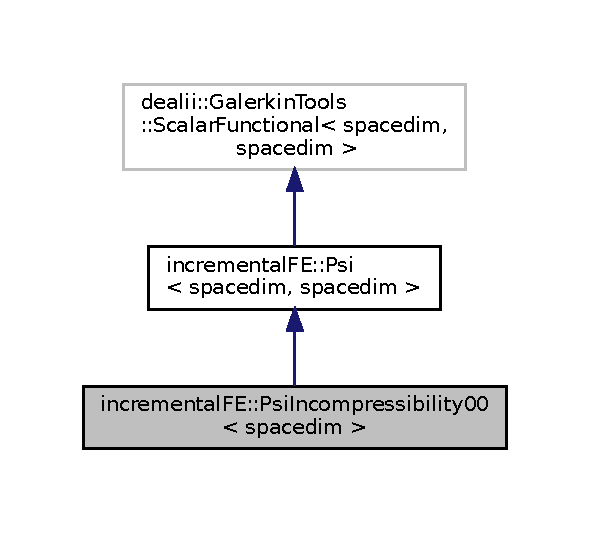
\includegraphics[width=264pt]{classincremental_f_e_1_1_psi_incompressibility00__inherit__graph}
\end{center}
\end{figure}


Collaboration diagram for incremental\+FE\+:\+:Psi\+Incompressibility00$<$ spacedim $>$\+:\nopagebreak
\begin{figure}[H]
\begin{center}
\leavevmode
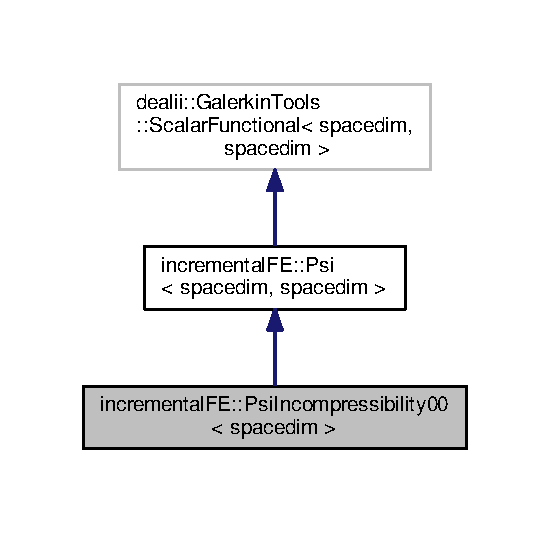
\includegraphics[width=264pt]{classincremental_f_e_1_1_psi_incompressibility00__coll__graph}
\end{center}
\end{figure}
\subsection*{Private Attributes}
\begin{DoxyCompactItemize}
\item 
const double \hyperlink{classincremental_f_e_1_1_psi_incompressibility00_adb4a98d91d9105e56d71b1c2bbb731fe}{V\+\_\+m\+\_\+f}
\item 
const double \hyperlink{classincremental_f_e_1_1_psi_incompressibility00_a21e9fc511e9410d0fbc9d0514f801f69}{n\+\_\+0}
\item 
const bool \hyperlink{classincremental_f_e_1_1_psi_incompressibility00_aca72a8996f35c7dbd664765af62dec95}{F\+\_\+as\+\_\+parameter}
\end{DoxyCompactItemize}
\subsection*{Additional Inherited Members}


\subsection{Detailed Description}
\subsubsection*{template$<$unsigned int spacedim$>$\\*
class incremental\+F\+E\+::\+Psi\+Incompressibility00$<$ spacedim $>$}

Class defining an incompressibility constraint for a hydrogel through the Lagrangian multiplier term

$h^\Omega_\rho = p\left( n_0 + c^\mathrm{f} V^\mathrm{f}_\mathrm{m} - J \right)$,

where $n_0$ is the initial concentration of the solid skeleton, $c^\mathrm{f}$ the fluid concentration, $V^\mathrm{f}_\mathrm{m}$ the molar volume of the fluid, and $J$ the determinant of the deformation gradient $\boldsymbol{F}$

Ordering of quantities in {\bf Scalar\+Functional$<$spacedim, spacedim$>$\+::e\+\_\+omega} \+:~\newline
 \mbox{[}0\mbox{]} $F_{xx}$~\newline
 \mbox{[}1\mbox{]} $F_{xy}$~\newline
 \mbox{[}2\mbox{]} $F_{xz}$~\newline
 \mbox{[}3\mbox{]} $F_{yx}$~\newline
 \mbox{[}4\mbox{]} $F_{yy}$~\newline
 \mbox{[}5\mbox{]} $F_{yz}$~\newline
 \mbox{[}6\mbox{]} $F_{zx}$~\newline
 \mbox{[}7\mbox{]} $F_{zy}$~\newline
 \mbox{[}8\mbox{]} $F_{zz}$~\newline
 \mbox{[}9\mbox{]} $c^\mathrm{f}$~\newline
 \mbox{[}10\mbox{]} $p$ 

\subsection{Member Data Documentation}
\index{incremental\+F\+E\+::\+Psi\+Incompressibility00@{incremental\+F\+E\+::\+Psi\+Incompressibility00}!F\+\_\+as\+\_\+parameter@{F\+\_\+as\+\_\+parameter}}
\index{F\+\_\+as\+\_\+parameter@{F\+\_\+as\+\_\+parameter}!incremental\+F\+E\+::\+Psi\+Incompressibility00@{incremental\+F\+E\+::\+Psi\+Incompressibility00}}
\subsubsection[{\texorpdfstring{F\+\_\+as\+\_\+parameter}{F_as_parameter}}]{\setlength{\rightskip}{0pt plus 5cm}template$<$unsigned int spacedim$>$ const bool {\bf incremental\+F\+E\+::\+Psi\+Incompressibility00}$<$ spacedim $>$\+::F\+\_\+as\+\_\+parameter\hspace{0.3cm}{\ttfamily [private]}}\hypertarget{classincremental_f_e_1_1_psi_incompressibility00_aca72a8996f35c7dbd664765af62dec95}{}\label{classincremental_f_e_1_1_psi_incompressibility00_aca72a8996f35c7dbd664765af62dec95}
If {\ttfamily true}, deformation gradient is considered as parameter in potential (i.\+e., it is held fixed when computing the first derivative) \index{incremental\+F\+E\+::\+Psi\+Incompressibility00@{incremental\+F\+E\+::\+Psi\+Incompressibility00}!n\+\_\+0@{n\+\_\+0}}
\index{n\+\_\+0@{n\+\_\+0}!incremental\+F\+E\+::\+Psi\+Incompressibility00@{incremental\+F\+E\+::\+Psi\+Incompressibility00}}
\subsubsection[{\texorpdfstring{n\+\_\+0}{n_0}}]{\setlength{\rightskip}{0pt plus 5cm}template$<$unsigned int spacedim$>$ const double {\bf incremental\+F\+E\+::\+Psi\+Incompressibility00}$<$ spacedim $>$\+::n\+\_\+0\hspace{0.3cm}{\ttfamily [private]}}\hypertarget{classincremental_f_e_1_1_psi_incompressibility00_a21e9fc511e9410d0fbc9d0514f801f69}{}\label{classincremental_f_e_1_1_psi_incompressibility00_a21e9fc511e9410d0fbc9d0514f801f69}
$n_0$ \index{incremental\+F\+E\+::\+Psi\+Incompressibility00@{incremental\+F\+E\+::\+Psi\+Incompressibility00}!V\+\_\+m\+\_\+f@{V\+\_\+m\+\_\+f}}
\index{V\+\_\+m\+\_\+f@{V\+\_\+m\+\_\+f}!incremental\+F\+E\+::\+Psi\+Incompressibility00@{incremental\+F\+E\+::\+Psi\+Incompressibility00}}
\subsubsection[{\texorpdfstring{V\+\_\+m\+\_\+f}{V_m_f}}]{\setlength{\rightskip}{0pt plus 5cm}template$<$unsigned int spacedim$>$ const double {\bf incremental\+F\+E\+::\+Psi\+Incompressibility00}$<$ spacedim $>$\+::V\+\_\+m\+\_\+f\hspace{0.3cm}{\ttfamily [private]}}\hypertarget{classincremental_f_e_1_1_psi_incompressibility00_adb4a98d91d9105e56d71b1c2bbb731fe}{}\label{classincremental_f_e_1_1_psi_incompressibility00_adb4a98d91d9105e56d71b1c2bbb731fe}
$V^\mathrm{f}_\mathrm{m}$ 

The documentation for this class was generated from the following file\+:\begin{DoxyCompactItemize}
\item 
/home/sst/code/\+Incremental\+F\+E/\+Incremental\+F\+E/include/incremental\+\_\+fe/scalar\+\_\+functionals/\hyperlink{psi__lib_8h}{psi\+\_\+lib.\+h}\end{DoxyCompactItemize}

\hypertarget{classincremental_f_e_1_1_psi_initial_pressure00}{}\section{incremental\+FE\+:\+:Psi\+Initial\+Pressure00$<$ spacedim $>$ Class Template Reference}
\label{classincremental_f_e_1_1_psi_initial_pressure00}\index{incremental\+F\+E\+::\+Psi\+Initial\+Pressure00$<$ spacedim $>$@{incremental\+F\+E\+::\+Psi\+Initial\+Pressure00$<$ spacedim $>$}}


{\ttfamily \#include $<$psi\+\_\+lib.\+h$>$}



Inheritance diagram for incremental\+FE\+:\+:Psi\+Initial\+Pressure00$<$ spacedim $>$\+:\nopagebreak
\begin{figure}[H]
\begin{center}
\leavevmode
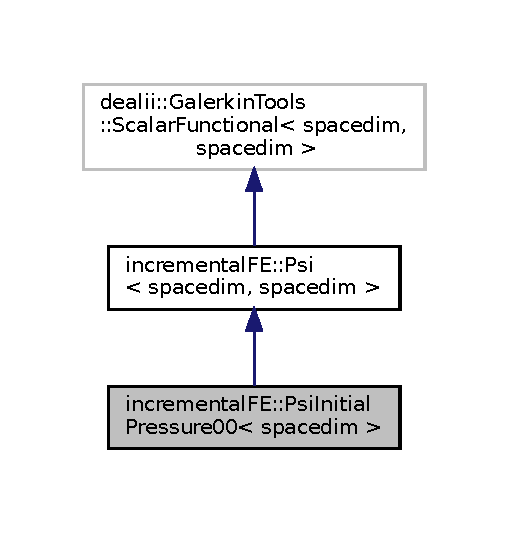
\includegraphics[width=229pt]{classincremental_f_e_1_1_psi_initial_pressure00__inherit__graph}
\end{center}
\end{figure}


Collaboration diagram for incremental\+FE\+:\+:Psi\+Initial\+Pressure00$<$ spacedim $>$\+:\nopagebreak
\begin{figure}[H]
\begin{center}
\leavevmode
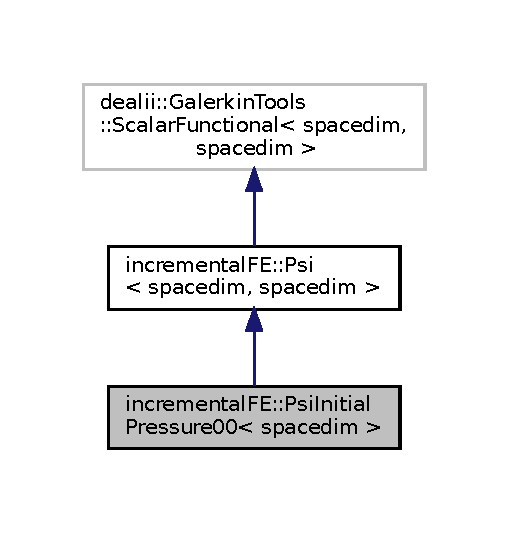
\includegraphics[width=229pt]{classincremental_f_e_1_1_psi_initial_pressure00__coll__graph}
\end{center}
\end{figure}
\subsection*{Public Member Functions}
\begin{DoxyCompactItemize}
\item 
\hyperlink{classincremental_f_e_1_1_psi_initial_pressure00_a5776a7b2766d5997b63e992df064fc73}{Psi\+Initial\+Pressure00} (const std\+::vector$<$ dealii\+::\+Galerkin\+Tools\+::\+Dependent\+Field$<$ spacedim, spacedim $>$$>$ e\+\_\+omega, const std\+::set$<$ {\bf dealii\+::types\+::material\+\_\+id} $>$ domain\+\_\+of\+\_\+integration, const dealii\+::\+Quadrature$<$ spacedim $>$ quadrature, \hyperlink{classincremental_f_e_1_1_global_data_incremental_f_e}{Global\+Data\+Incremental\+FE}$<$ spacedim $>$ \&\hyperlink{classincremental_f_e_1_1_psi_3_01spacedim_00_01spacedim_01_4_abf0a4804877fd7cc9bd1b90e52760ba9}{global\+\_\+data}, const double \hyperlink{classincremental_f_e_1_1_psi_initial_pressure00_a8acf3825dbfea2fe0e0ebc5711b93fca}{p\+\_\+0}, const double \hyperlink{classincremental_f_e_1_1_psi_3_01spacedim_00_01spacedim_01_4_af7b8227188dbdd6ada35b9445d96c79d}{alpha})
\item 
bool \hyperlink{classincremental_f_e_1_1_psi_initial_pressure00_aeb78a4eb41e692ff1b0f75f2695858fb}{get\+\_\+values\+\_\+and\+\_\+derivatives} (const {\bf dealii\+::\+Vector}$<$ double $>$ \&{\bf values}, const dealii\+::\+Point$<$ spacedim $>$ \&, double \&omega, {\bf dealii\+::\+Vector}$<$ double $>$ \&d\+\_\+omega, dealii\+::\+Full\+Matrix$<$ double $>$ \&d2\+\_\+omega, const std\+::tuple$<$ bool, bool, bool $>$ requested\+\_\+quantities) const 
\end{DoxyCompactItemize}
\subsection*{Private Attributes}
\begin{DoxyCompactItemize}
\item 
const double \hyperlink{classincremental_f_e_1_1_psi_initial_pressure00_a8acf3825dbfea2fe0e0ebc5711b93fca}{p\+\_\+0}
\end{DoxyCompactItemize}


\subsection{Detailed Description}
\subsubsection*{template$<$unsigned int spacedim$>$\\*
class incremental\+F\+E\+::\+Psi\+Initial\+Pressure00$<$ spacedim $>$}

Class defining an initial pressure term

$h^\Omega_\rho = p_0 J$,

where $p_0$ is the (constant) initial pressure, and $J$ the determinant of the deformation gradient $\boldsymbol{F}$

Ordering of quantities in {\bf Scalar\+Functional$<$spacedim, spacedim$>$\+::e\+\_\+omega} \+:~\newline
 \mbox{[}0\mbox{]} $F_{xx}$~\newline
 \mbox{[}1\mbox{]} $F_{xy}$~\newline
 \mbox{[}2\mbox{]} $F_{xz}$~\newline
 \mbox{[}3\mbox{]} $F_{yx}$~\newline
 \mbox{[}4\mbox{]} $F_{yy}$~\newline
 \mbox{[}5\mbox{]} $F_{yz}$~\newline
 \mbox{[}6\mbox{]} $F_{zx}$~\newline
 \mbox{[}7\mbox{]} $F_{zy}$~\newline
 \mbox{[}8\mbox{]} $F_{zz}$~\newline
 

\subsection{Constructor \& Destructor Documentation}
\index{incremental\+F\+E\+::\+Psi\+Initial\+Pressure00@{incremental\+F\+E\+::\+Psi\+Initial\+Pressure00}!Psi\+Initial\+Pressure00@{Psi\+Initial\+Pressure00}}
\index{Psi\+Initial\+Pressure00@{Psi\+Initial\+Pressure00}!incremental\+F\+E\+::\+Psi\+Initial\+Pressure00@{incremental\+F\+E\+::\+Psi\+Initial\+Pressure00}}
\subsubsection[{\texorpdfstring{Psi\+Initial\+Pressure00(const std\+::vector$<$ dealii\+::\+Galerkin\+Tools\+::\+Dependent\+Field$<$ spacedim, spacedim $>$$>$ e\+\_\+omega, const std\+::set$<$ dealii\+::types\+::material\+\_\+id $>$ domain\+\_\+of\+\_\+integration, const dealii\+::\+Quadrature$<$ spacedim $>$ quadrature, Global\+Data\+Incremental\+F\+E$<$ spacedim $>$ \&global\+\_\+data, const double p\+\_\+0, const double alpha)}{PsiInitialPressure00(const std::vector< dealii::GalerkinTools::DependentField< spacedim, spacedim >> e_omega, const std::set< dealii::types::material_id > domain_of_integration, const dealii::Quadrature< spacedim > quadrature, GlobalDataIncrementalFE< spacedim > &global_data, const double p_0, const double alpha)}}]{\setlength{\rightskip}{0pt plus 5cm}template$<$unsigned int spacedim$>$ {\bf incremental\+F\+E\+::\+Psi\+Initial\+Pressure00}$<$ spacedim $>$\+::{\bf Psi\+Initial\+Pressure00} (
\begin{DoxyParamCaption}
\item[{const std\+::vector$<$ dealii\+::\+Galerkin\+Tools\+::\+Dependent\+Field$<$ spacedim, spacedim $>$$>$}]{e\+\_\+omega, }
\item[{const std\+::set$<$ {\bf dealii\+::types\+::material\+\_\+id} $>$}]{domain\+\_\+of\+\_\+integration, }
\item[{const dealii\+::\+Quadrature$<$ spacedim $>$}]{quadrature, }
\item[{{\bf Global\+Data\+Incremental\+FE}$<$ spacedim $>$ \&}]{global\+\_\+data, }
\item[{const double}]{p\+\_\+0, }
\item[{const double}]{alpha}
\end{DoxyParamCaption}
)\hspace{0.3cm}{\ttfamily [inline]}}\hypertarget{classincremental_f_e_1_1_psi_initial_pressure00_a5776a7b2766d5997b63e992df064fc73}{}\label{classincremental_f_e_1_1_psi_initial_pressure00_a5776a7b2766d5997b63e992df064fc73}
Constructor


\begin{DoxyParams}[1]{Parameters}
\mbox{\tt in}  & {\em e\+\_\+omega} & {\bf Scalar\+Functional$<$spacedim, spacedim$>$\+::e\+\_\+omega}\\
\hline
\mbox{\tt in}  & {\em domain\+\_\+of\+\_\+integration} & {\bf Scalar\+Functional$<$spacedim, spacedim$>$\+::domain\+\_\+of\+\_\+integration}\\
\hline
\mbox{\tt in}  & {\em quadrature} & {\bf Scalar\+Functional$<$spacedim, spacedim$>$\+::quadrature}\\
\hline
\mbox{\tt in}  & {\em global\+\_\+data} & \hyperlink{classincremental_f_e_1_1_psi_3_01spacedim_00_01spacedim_01_4_abf0a4804877fd7cc9bd1b90e52760ba9}{Psi$<$spacedim, spacedim$>$\+::global\+\_\+data}\\
\hline
\mbox{\tt in}  & {\em p\+\_\+0} & \hyperlink{classincremental_f_e_1_1_psi_initial_pressure00_a8acf3825dbfea2fe0e0ebc5711b93fca}{Psi\+Initial\+Pressure00\+::p\+\_\+0}\\
\hline
\mbox{\tt in}  & {\em alpha} & \hyperlink{classincremental_f_e_1_1_psi_3_01spacedim_00_01spacedim_01_4_af7b8227188dbdd6ada35b9445d96c79d}{Psi$<$spacedim, spacedim$>$\+::alpha} \\
\hline
\end{DoxyParams}


\subsection{Member Function Documentation}
\index{incremental\+F\+E\+::\+Psi\+Initial\+Pressure00@{incremental\+F\+E\+::\+Psi\+Initial\+Pressure00}!get\+\_\+values\+\_\+and\+\_\+derivatives@{get\+\_\+values\+\_\+and\+\_\+derivatives}}
\index{get\+\_\+values\+\_\+and\+\_\+derivatives@{get\+\_\+values\+\_\+and\+\_\+derivatives}!incremental\+F\+E\+::\+Psi\+Initial\+Pressure00@{incremental\+F\+E\+::\+Psi\+Initial\+Pressure00}}
\subsubsection[{\texorpdfstring{get\+\_\+values\+\_\+and\+\_\+derivatives(const dealii\+::\+Vector$<$ double $>$ \&values, const dealii\+::\+Point$<$ spacedim $>$ \&, double \&omega, dealii\+::\+Vector$<$ double $>$ \&d\+\_\+omega, dealii\+::\+Full\+Matrix$<$ double $>$ \&d2\+\_\+omega, const std\+::tuple$<$ bool, bool, bool $>$ requested\+\_\+quantities) const }{get_values_and_derivatives(const dealii::Vector< double > &values, const dealii::Point< spacedim > &, double &omega, dealii::Vector< double > &d_omega, dealii::FullMatrix< double > &d2_omega, const std::tuple< bool, bool, bool > requested_quantities) const }}]{\setlength{\rightskip}{0pt plus 5cm}template$<$unsigned int spacedim$>$ bool {\bf incremental\+F\+E\+::\+Psi\+Initial\+Pressure00}$<$ spacedim $>$\+::get\+\_\+values\+\_\+and\+\_\+derivatives (
\begin{DoxyParamCaption}
\item[{const {\bf dealii\+::\+Vector}$<$ double $>$ \&}]{values, }
\item[{const dealii\+::\+Point$<$ spacedim $>$ \&}]{, }
\item[{double \&}]{omega, }
\item[{{\bf dealii\+::\+Vector}$<$ double $>$ \&}]{d\+\_\+omega, }
\item[{dealii\+::\+Full\+Matrix$<$ double $>$ \&}]{d2\+\_\+omega, }
\item[{const std\+::tuple$<$ bool, bool, bool $>$}]{requested\+\_\+quantities}
\end{DoxyParamCaption}
) const\hspace{0.3cm}{\ttfamily [inline]}, {\ttfamily [virtual]}}\hypertarget{classincremental_f_e_1_1_psi_initial_pressure00_aeb78a4eb41e692ff1b0f75f2695858fb}{}\label{classincremental_f_e_1_1_psi_initial_pressure00_aeb78a4eb41e692ff1b0f75f2695858fb}
\begin{DoxySeeAlso}{See also}
\hyperlink{classincremental_f_e_1_1_psi_3_01spacedim_00_01spacedim_01_4_a17f3559c196edb5487b591bb6061667e}{Psi$<$spacedim, spacedim$>$\+::get\+\_\+values\+\_\+and\+\_\+derivatives()} 
\end{DoxySeeAlso}


Implements \hyperlink{classincremental_f_e_1_1_psi_3_01spacedim_00_01spacedim_01_4_a17f3559c196edb5487b591bb6061667e}{incremental\+F\+E\+::\+Psi$<$ spacedim, spacedim $>$}.



\subsection{Member Data Documentation}
\index{incremental\+F\+E\+::\+Psi\+Initial\+Pressure00@{incremental\+F\+E\+::\+Psi\+Initial\+Pressure00}!p\+\_\+0@{p\+\_\+0}}
\index{p\+\_\+0@{p\+\_\+0}!incremental\+F\+E\+::\+Psi\+Initial\+Pressure00@{incremental\+F\+E\+::\+Psi\+Initial\+Pressure00}}
\subsubsection[{\texorpdfstring{p\+\_\+0}{p_0}}]{\setlength{\rightskip}{0pt plus 5cm}template$<$unsigned int spacedim$>$ const double {\bf incremental\+F\+E\+::\+Psi\+Initial\+Pressure00}$<$ spacedim $>$\+::p\+\_\+0\hspace{0.3cm}{\ttfamily [private]}}\hypertarget{classincremental_f_e_1_1_psi_initial_pressure00_a8acf3825dbfea2fe0e0ebc5711b93fca}{}\label{classincremental_f_e_1_1_psi_initial_pressure00_a8acf3825dbfea2fe0e0ebc5711b93fca}
$p_0$ 

The documentation for this class was generated from the following file\+:\begin{DoxyCompactItemize}
\item 
/home/sst/code/\+Incremental\+F\+E/\+Incremental\+F\+E/include/incremental\+\_\+fe/scalar\+\_\+functionals/\hyperlink{psi__lib_8h}{psi\+\_\+lib.\+h}\end{DoxyCompactItemize}

\hypertarget{classincremental_f_e_1_1_psi_linear00}{}\section{incremental\+FE\+:\+:Psi\+Linear00$<$ spacedim $>$ Class Template Reference}
\label{classincremental_f_e_1_1_psi_linear00}\index{incremental\+F\+E\+::\+Psi\+Linear00$<$ spacedim $>$@{incremental\+F\+E\+::\+Psi\+Linear00$<$ spacedim $>$}}


{\ttfamily \#include $<$psi\+\_\+lib.\+h$>$}



Inheritance diagram for incremental\+FE\+:\+:Psi\+Linear00$<$ spacedim $>$\+:\nopagebreak
\begin{figure}[H]
\begin{center}
\leavevmode
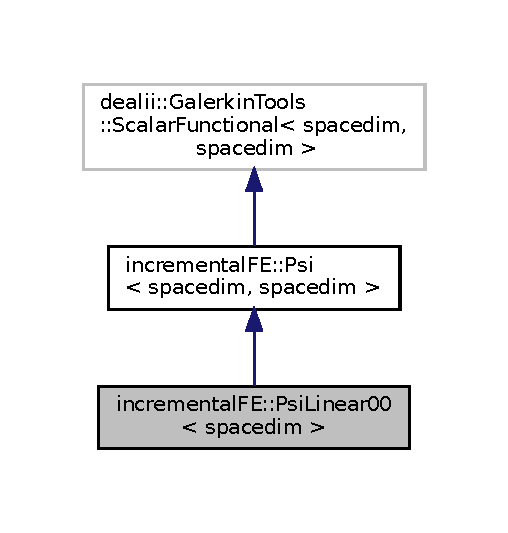
\includegraphics[width=229pt]{classincremental_f_e_1_1_psi_linear00__inherit__graph}
\end{center}
\end{figure}


Collaboration diagram for incremental\+FE\+:\+:Psi\+Linear00$<$ spacedim $>$\+:\nopagebreak
\begin{figure}[H]
\begin{center}
\leavevmode
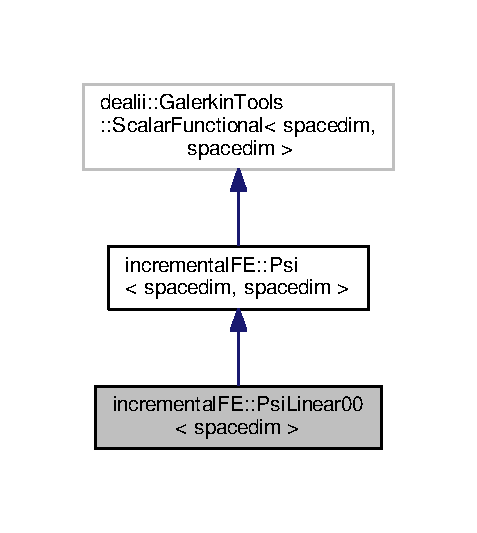
\includegraphics[width=229pt]{classincremental_f_e_1_1_psi_linear00__coll__graph}
\end{center}
\end{figure}
\subsection*{Public Member Functions}
\begin{DoxyCompactItemize}
\item 
\hyperlink{classincremental_f_e_1_1_psi_linear00_aa5dbe1b55411bfc642c4c9ed2508eefe}{Psi\+Linear00} (const std\+::vector$<$ dealii\+::\+Galerkin\+Tools\+::\+Dependent\+Field$<$ spacedim, spacedim $>$$>$ e\+\_\+omega, const std\+::set$<$ {\bf dealii\+::types\+::material\+\_\+id} $>$ domain\+\_\+of\+\_\+integration, const dealii\+::\+Quadrature$<$ spacedim $>$ quadrature, \hyperlink{classincremental_f_e_1_1_global_data_incremental_f_e}{Global\+Data\+Incremental\+FE}$<$ spacedim $>$ \&\hyperlink{classincremental_f_e_1_1_psi_3_01spacedim_00_01spacedim_01_4_abf0a4804877fd7cc9bd1b90e52760ba9}{global\+\_\+data}, const dealii\+::\+Full\+Matrix$<$ double $>$ \&\hyperlink{classincremental_f_e_1_1_psi_linear00_a6d4534350ad8b74c6930c3afa1031801}{A}, const {\bf dealii\+::\+Vector}$<$ double $>$ \&\hyperlink{classincremental_f_e_1_1_psi_linear00_ab16d4f5295fc2637f0f7662843d4cac1}{b}, const double \hyperlink{classincremental_f_e_1_1_psi_3_01spacedim_00_01spacedim_01_4_af7b8227188dbdd6ada35b9445d96c79d}{alpha})
\item 
bool \hyperlink{classincremental_f_e_1_1_psi_linear00_ac2fdec793550c0f26808e02d9d17b889}{get\+\_\+values\+\_\+and\+\_\+derivatives} (const {\bf dealii\+::\+Vector}$<$ double $>$ \&{\bf values}, const dealii\+::\+Point$<$ spacedim $>$ \&, double \&omega, {\bf dealii\+::\+Vector}$<$ double $>$ \&d\+\_\+omega, dealii\+::\+Full\+Matrix$<$ double $>$ \&d2\+\_\+omega, const std\+::tuple$<$ bool, bool, bool $>$ requested\+\_\+quantities) const 
\end{DoxyCompactItemize}
\subsection*{Private Attributes}
\begin{DoxyCompactItemize}
\item 
const dealii\+::\+Full\+Matrix$<$ double $>$ \hyperlink{classincremental_f_e_1_1_psi_linear00_a6d4534350ad8b74c6930c3afa1031801}{A}
\item 
const {\bf dealii\+::\+Vector}$<$ double $>$ \hyperlink{classincremental_f_e_1_1_psi_linear00_ab16d4f5295fc2637f0f7662843d4cac1}{b}
\end{DoxyCompactItemize}


\subsection{Detailed Description}
\subsubsection*{template$<$unsigned int spacedim$>$\\*
class incremental\+F\+E\+::\+Psi\+Linear00$<$ spacedim $>$}

Class defining a domain related scalar functional with the integrand

$h^\Omega_\rho = 1/2 q A q + b q$,

where $q$ is a state variable, and $A$ and $b$ are constants. The implementation works also for vector valued $q$, in which case $A$ is a matrix and $b$ a vector.

Ordering of quantities in {\bf Scalar\+Functional$<$spacedim, spacedim$>$\+::e\+\_\+omega} \+:~\newline
 \mbox{[}0\mbox{]} $q$ 

\subsection{Constructor \& Destructor Documentation}
\index{incremental\+F\+E\+::\+Psi\+Linear00@{incremental\+F\+E\+::\+Psi\+Linear00}!Psi\+Linear00@{Psi\+Linear00}}
\index{Psi\+Linear00@{Psi\+Linear00}!incremental\+F\+E\+::\+Psi\+Linear00@{incremental\+F\+E\+::\+Psi\+Linear00}}
\subsubsection[{\texorpdfstring{Psi\+Linear00(const std\+::vector$<$ dealii\+::\+Galerkin\+Tools\+::\+Dependent\+Field$<$ spacedim, spacedim $>$$>$ e\+\_\+omega, const std\+::set$<$ dealii\+::types\+::material\+\_\+id $>$ domain\+\_\+of\+\_\+integration, const dealii\+::\+Quadrature$<$ spacedim $>$ quadrature, Global\+Data\+Incremental\+F\+E$<$ spacedim $>$ \&global\+\_\+data, const dealii\+::\+Full\+Matrix$<$ double $>$ \&\+A, const dealii\+::\+Vector$<$ double $>$ \&b, const double alpha)}{PsiLinear00(const std::vector< dealii::GalerkinTools::DependentField< spacedim, spacedim >> e_omega, const std::set< dealii::types::material_id > domain_of_integration, const dealii::Quadrature< spacedim > quadrature, GlobalDataIncrementalFE< spacedim > &global_data, const dealii::FullMatrix< double > &A, const dealii::Vector< double > &b, const double alpha)}}]{\setlength{\rightskip}{0pt plus 5cm}template$<$unsigned int spacedim$>$ {\bf incremental\+F\+E\+::\+Psi\+Linear00}$<$ spacedim $>$\+::{\bf Psi\+Linear00} (
\begin{DoxyParamCaption}
\item[{const std\+::vector$<$ dealii\+::\+Galerkin\+Tools\+::\+Dependent\+Field$<$ spacedim, spacedim $>$$>$}]{e\+\_\+omega, }
\item[{const std\+::set$<$ {\bf dealii\+::types\+::material\+\_\+id} $>$}]{domain\+\_\+of\+\_\+integration, }
\item[{const dealii\+::\+Quadrature$<$ spacedim $>$}]{quadrature, }
\item[{{\bf Global\+Data\+Incremental\+FE}$<$ spacedim $>$ \&}]{global\+\_\+data, }
\item[{const dealii\+::\+Full\+Matrix$<$ double $>$ \&}]{A, }
\item[{const {\bf dealii\+::\+Vector}$<$ double $>$ \&}]{b, }
\item[{const double}]{alpha}
\end{DoxyParamCaption}
)\hspace{0.3cm}{\ttfamily [inline]}}\hypertarget{classincremental_f_e_1_1_psi_linear00_aa5dbe1b55411bfc642c4c9ed2508eefe}{}\label{classincremental_f_e_1_1_psi_linear00_aa5dbe1b55411bfc642c4c9ed2508eefe}
Constructor


\begin{DoxyParams}[1]{Parameters}
\mbox{\tt in}  & {\em e\+\_\+omega} & {\bf Scalar\+Functional$<$spacedim, spacedim$>$\+::e\+\_\+omega}\\
\hline
\mbox{\tt in}  & {\em domain\+\_\+of\+\_\+integration} & {\bf Scalar\+Functional$<$spacedim, spacedim$>$\+::domain\+\_\+of\+\_\+integration}\\
\hline
\mbox{\tt in}  & {\em quadrature} & {\bf Scalar\+Functional$<$spacedim, spacedim$>$\+::quadrature}\\
\hline
\mbox{\tt in}  & {\em global\+\_\+data} & \hyperlink{classincremental_f_e_1_1_psi_3_01spacedim_00_01spacedim_01_4_abf0a4804877fd7cc9bd1b90e52760ba9}{Psi$<$spacedim, spacedim$>$\+::global\+\_\+data}\\
\hline
\mbox{\tt in}  & {\em A} & \hyperlink{classincremental_f_e_1_1_psi_linear00_a6d4534350ad8b74c6930c3afa1031801}{Psi\+Linear00\+::A}\\
\hline
\mbox{\tt in}  & {\em b} & \hyperlink{classincremental_f_e_1_1_psi_linear00_ab16d4f5295fc2637f0f7662843d4cac1}{Psi\+Linear00\+::b}\\
\hline
\mbox{\tt in}  & {\em alpha} & \hyperlink{classincremental_f_e_1_1_psi_3_01spacedim_00_01spacedim_01_4_af7b8227188dbdd6ada35b9445d96c79d}{Psi$<$spacedim, spacedim$>$\+::alpha} \\
\hline
\end{DoxyParams}


\subsection{Member Function Documentation}
\index{incremental\+F\+E\+::\+Psi\+Linear00@{incremental\+F\+E\+::\+Psi\+Linear00}!get\+\_\+values\+\_\+and\+\_\+derivatives@{get\+\_\+values\+\_\+and\+\_\+derivatives}}
\index{get\+\_\+values\+\_\+and\+\_\+derivatives@{get\+\_\+values\+\_\+and\+\_\+derivatives}!incremental\+F\+E\+::\+Psi\+Linear00@{incremental\+F\+E\+::\+Psi\+Linear00}}
\subsubsection[{\texorpdfstring{get\+\_\+values\+\_\+and\+\_\+derivatives(const dealii\+::\+Vector$<$ double $>$ \&values, const dealii\+::\+Point$<$ spacedim $>$ \&, double \&omega, dealii\+::\+Vector$<$ double $>$ \&d\+\_\+omega, dealii\+::\+Full\+Matrix$<$ double $>$ \&d2\+\_\+omega, const std\+::tuple$<$ bool, bool, bool $>$ requested\+\_\+quantities) const }{get_values_and_derivatives(const dealii::Vector< double > &values, const dealii::Point< spacedim > &, double &omega, dealii::Vector< double > &d_omega, dealii::FullMatrix< double > &d2_omega, const std::tuple< bool, bool, bool > requested_quantities) const }}]{\setlength{\rightskip}{0pt plus 5cm}template$<$unsigned int spacedim$>$ bool {\bf incremental\+F\+E\+::\+Psi\+Linear00}$<$ spacedim $>$\+::get\+\_\+values\+\_\+and\+\_\+derivatives (
\begin{DoxyParamCaption}
\item[{const {\bf dealii\+::\+Vector}$<$ double $>$ \&}]{values, }
\item[{const dealii\+::\+Point$<$ spacedim $>$ \&}]{, }
\item[{double \&}]{omega, }
\item[{{\bf dealii\+::\+Vector}$<$ double $>$ \&}]{d\+\_\+omega, }
\item[{dealii\+::\+Full\+Matrix$<$ double $>$ \&}]{d2\+\_\+omega, }
\item[{const std\+::tuple$<$ bool, bool, bool $>$}]{requested\+\_\+quantities}
\end{DoxyParamCaption}
) const\hspace{0.3cm}{\ttfamily [inline]}, {\ttfamily [virtual]}}\hypertarget{classincremental_f_e_1_1_psi_linear00_ac2fdec793550c0f26808e02d9d17b889}{}\label{classincremental_f_e_1_1_psi_linear00_ac2fdec793550c0f26808e02d9d17b889}
\begin{DoxySeeAlso}{See also}
\hyperlink{classincremental_f_e_1_1_psi_3_01spacedim_00_01spacedim_01_4_a17f3559c196edb5487b591bb6061667e}{Psi$<$spacedim, spacedim$>$\+::get\+\_\+values\+\_\+and\+\_\+derivatives()} 
\end{DoxySeeAlso}


Implements \hyperlink{classincremental_f_e_1_1_psi_3_01spacedim_00_01spacedim_01_4_a17f3559c196edb5487b591bb6061667e}{incremental\+F\+E\+::\+Psi$<$ spacedim, spacedim $>$}.



\subsection{Member Data Documentation}
\index{incremental\+F\+E\+::\+Psi\+Linear00@{incremental\+F\+E\+::\+Psi\+Linear00}!A@{A}}
\index{A@{A}!incremental\+F\+E\+::\+Psi\+Linear00@{incremental\+F\+E\+::\+Psi\+Linear00}}
\subsubsection[{\texorpdfstring{A}{A}}]{\setlength{\rightskip}{0pt plus 5cm}template$<$unsigned int spacedim$>$ const dealii\+::\+Full\+Matrix$<$double$>$ {\bf incremental\+F\+E\+::\+Psi\+Linear00}$<$ spacedim $>$\+::A\hspace{0.3cm}{\ttfamily [private]}}\hypertarget{classincremental_f_e_1_1_psi_linear00_a6d4534350ad8b74c6930c3afa1031801}{}\label{classincremental_f_e_1_1_psi_linear00_a6d4534350ad8b74c6930c3afa1031801}
Matrix $A$ \index{incremental\+F\+E\+::\+Psi\+Linear00@{incremental\+F\+E\+::\+Psi\+Linear00}!b@{b}}
\index{b@{b}!incremental\+F\+E\+::\+Psi\+Linear00@{incremental\+F\+E\+::\+Psi\+Linear00}}
\subsubsection[{\texorpdfstring{b}{b}}]{\setlength{\rightskip}{0pt plus 5cm}template$<$unsigned int spacedim$>$ const {\bf dealii\+::\+Vector}$<$double$>$ {\bf incremental\+F\+E\+::\+Psi\+Linear00}$<$ spacedim $>$\+::b\hspace{0.3cm}{\ttfamily [private]}}\hypertarget{classincremental_f_e_1_1_psi_linear00_ab16d4f5295fc2637f0f7662843d4cac1}{}\label{classincremental_f_e_1_1_psi_linear00_ab16d4f5295fc2637f0f7662843d4cac1}
Vector $b$ 

The documentation for this class was generated from the following file\+:\begin{DoxyCompactItemize}
\item 
/home/sst/code/\+Incremental\+F\+E/\+Incremental\+F\+E/include/incremental\+\_\+fe/scalar\+\_\+functionals/\hyperlink{psi__lib_8h}{psi\+\_\+lib.\+h}\end{DoxyCompactItemize}

\hypertarget{classincremental_f_e_1_1_psi_linear_interface00}{}\doxysection{incremental\+FE\+::Psi\+Linear\+Interface00$<$ spacedim $>$ Class Template Reference}
\label{classincremental_f_e_1_1_psi_linear_interface00}\index{incrementalFE::PsiLinearInterface00$<$ spacedim $>$@{incrementalFE::PsiLinearInterface00$<$ spacedim $>$}}


{\ttfamily \#include $<$psi\+\_\+lib.\+h$>$}



Inheritance diagram for incremental\+FE\+::Psi\+Linear\+Interface00$<$ spacedim $>$\+:\nopagebreak
\begin{figure}[H]
\begin{center}
\leavevmode
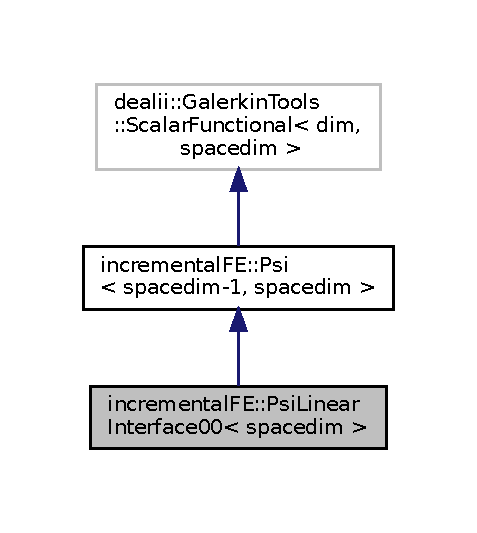
\includegraphics[width=229pt]{classincremental_f_e_1_1_psi_linear_interface00__inherit__graph}
\end{center}
\end{figure}


Collaboration diagram for incremental\+FE\+::Psi\+Linear\+Interface00$<$ spacedim $>$\+:\nopagebreak
\begin{figure}[H]
\begin{center}
\leavevmode
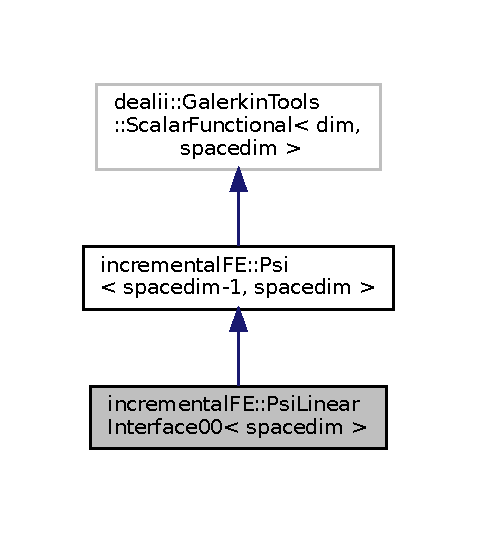
\includegraphics[width=229pt]{classincremental_f_e_1_1_psi_linear_interface00__coll__graph}
\end{center}
\end{figure}
\doxysubsection*{Public Member Functions}
\begin{DoxyCompactItemize}
\item 
\mbox{\hyperlink{classincremental_f_e_1_1_psi_linear_interface00_a0044414c2ebe5dd31faae421ec5f6383}{Psi\+Linear\+Interface00}} (const std\+::vector$<$ dealii\+::\+Galerkin\+Tools\+::\+Dependent\+Field$<$ spacedim-\/1, spacedim $>$$>$ e\+\_\+sigma, const std\+::set$<$ \textbf{ dealii\+::types\+::material\+\_\+id} $>$ domain\+\_\+of\+\_\+integration, const dealii\+::\+Quadrature$<$ spacedim-\/1 $>$ quadrature, \mbox{\hyperlink{classincremental_f_e_1_1_global_data_incremental_f_e}{Global\+Data\+Incremental\+FE}}$<$ spacedim $>$ \&\mbox{\hyperlink{classincremental_f_e_1_1_psi_ae77b2e13385734b19d6ee445c477a6eb}{global\+\_\+data}}, const dealii\+::\+Full\+Matrix$<$ double $>$ \&\mbox{\hyperlink{classincremental_f_e_1_1_psi_linear_interface00_a58c4e916fb9d722b16963e213235ed81}{A}}, const \textbf{ dealii\+::\+Vector}$<$ double $>$ \&\mbox{\hyperlink{classincremental_f_e_1_1_psi_linear_interface00_a67da23f105ba3e30884099c71c972b56}{b}}, const double \mbox{\hyperlink{classincremental_f_e_1_1_psi_a5112e8bd1a2d5230d39937f16466d76f}{alpha}})
\item 
bool \mbox{\hyperlink{classincremental_f_e_1_1_psi_linear_interface00_a5484f908e32ff84cc12501a33243f30f}{get\+\_\+values\+\_\+and\+\_\+derivatives}} (const \textbf{ dealii\+::\+Vector}$<$ double $>$ \&\textbf{ values}, const dealii\+::\+Point$<$ spacedim $>$ \&, const dealii\+::\+Tensor$<$ 1, spacedim $>$ \&, double \&sigma, \textbf{ dealii\+::\+Vector}$<$ double $>$ \&d\+\_\+sigma, dealii\+::\+Full\+Matrix$<$ double $>$ \&d2\+\_\+sigma, const std\+::tuple$<$ bool, bool, bool $>$ requested\+\_\+quantities) const
\end{DoxyCompactItemize}
\doxysubsection*{Private Attributes}
\begin{DoxyCompactItemize}
\item 
const dealii\+::\+Full\+Matrix$<$ double $>$ \mbox{\hyperlink{classincremental_f_e_1_1_psi_linear_interface00_a58c4e916fb9d722b16963e213235ed81}{A}}
\item 
const \textbf{ dealii\+::\+Vector}$<$ double $>$ \mbox{\hyperlink{classincremental_f_e_1_1_psi_linear_interface00_a67da23f105ba3e30884099c71c972b56}{b}}
\end{DoxyCompactItemize}
\doxysubsection*{Additional Inherited Members}


\doxysubsection{Detailed Description}
\subsubsection*{template$<$unsigned int spacedim$>$\newline
class incremental\+F\+E\+::\+Psi\+Linear\+Interface00$<$ spacedim $>$}

Class defining an interface related scalar functional with the integrand

$h^\Sigma_\tau = 1/2 q A q + b q$,

where $q$ is a state variable, and $A$ and $b$ are constants. The implementation works also for vector valued $q$, in which case $A$ is a matrix and $b$ a vector.

Ordering of quantities in \textbf{ Scalar\+Functional\+::e\+\_\+sigma} \+:~\newline
 \mbox{[}0\mbox{]} $q$ 

\doxysubsection{Constructor \& Destructor Documentation}
\mbox{\Hypertarget{classincremental_f_e_1_1_psi_linear_interface00_a0044414c2ebe5dd31faae421ec5f6383}\label{classincremental_f_e_1_1_psi_linear_interface00_a0044414c2ebe5dd31faae421ec5f6383}} 
\index{incrementalFE::PsiLinearInterface00$<$ spacedim $>$@{incrementalFE::PsiLinearInterface00$<$ spacedim $>$}!PsiLinearInterface00@{PsiLinearInterface00}}
\index{PsiLinearInterface00@{PsiLinearInterface00}!incrementalFE::PsiLinearInterface00$<$ spacedim $>$@{incrementalFE::PsiLinearInterface00$<$ spacedim $>$}}
\doxysubsubsection{\texorpdfstring{PsiLinearInterface00()}{PsiLinearInterface00()}}
{\footnotesize\ttfamily template$<$unsigned int spacedim$>$ \\
\mbox{\hyperlink{classincremental_f_e_1_1_psi_linear_interface00}{incremental\+F\+E\+::\+Psi\+Linear\+Interface00}}$<$ spacedim $>$\+::\mbox{\hyperlink{classincremental_f_e_1_1_psi_linear_interface00}{Psi\+Linear\+Interface00}} (\begin{DoxyParamCaption}\item[{const std\+::vector$<$ dealii\+::\+Galerkin\+Tools\+::\+Dependent\+Field$<$ spacedim-\/1, spacedim $>$$>$}]{e\+\_\+sigma,  }\item[{const std\+::set$<$ \textbf{ dealii\+::types\+::material\+\_\+id} $>$}]{domain\+\_\+of\+\_\+integration,  }\item[{const dealii\+::\+Quadrature$<$ spacedim-\/1 $>$}]{quadrature,  }\item[{\mbox{\hyperlink{classincremental_f_e_1_1_global_data_incremental_f_e}{Global\+Data\+Incremental\+FE}}$<$ spacedim $>$ \&}]{global\+\_\+data,  }\item[{const dealii\+::\+Full\+Matrix$<$ double $>$ \&}]{A,  }\item[{const \textbf{ dealii\+::\+Vector}$<$ double $>$ \&}]{b,  }\item[{const double}]{alpha }\end{DoxyParamCaption})\hspace{0.3cm}{\ttfamily [inline]}}

Constructor


\begin{DoxyParams}[1]{Parameters}
\mbox{\texttt{ in}}  & {\em e\+\_\+sigma} & Scalar\+Functional\+::e\+\_\+omega\\
\hline
\mbox{\texttt{ in}}  & {\em domain\+\_\+of\+\_\+integration} & \textbf{ Scalar\+Functional\+::domain\+\_\+of\+\_\+integration}\\
\hline
\mbox{\texttt{ in}}  & {\em quadrature} & \textbf{ Scalar\+Functional\+::quadrature}\\
\hline
\mbox{\texttt{ in}}  & {\em global\+\_\+data} & \mbox{\hyperlink{classincremental_f_e_1_1_psi_ae77b2e13385734b19d6ee445c477a6eb}{Psi\+::global\+\_\+data}}\\
\hline
\mbox{\texttt{ in}}  & {\em A} & \mbox{\hyperlink{classincremental_f_e_1_1_psi_linear00_a6d4534350ad8b74c6930c3afa1031801}{Psi\+Linear00\+::A}}\\
\hline
\mbox{\texttt{ in}}  & {\em b} & \mbox{\hyperlink{classincremental_f_e_1_1_psi_linear00_ab16d4f5295fc2637f0f7662843d4cac1}{Psi\+Linear00\+::b}}\\
\hline
\mbox{\texttt{ in}}  & {\em alpha} & \mbox{\hyperlink{classincremental_f_e_1_1_psi_a5112e8bd1a2d5230d39937f16466d76f}{Psi\+::alpha}} \\
\hline
\end{DoxyParams}


\doxysubsection{Member Function Documentation}
\mbox{\Hypertarget{classincremental_f_e_1_1_psi_linear_interface00_a5484f908e32ff84cc12501a33243f30f}\label{classincremental_f_e_1_1_psi_linear_interface00_a5484f908e32ff84cc12501a33243f30f}} 
\index{incrementalFE::PsiLinearInterface00$<$ spacedim $>$@{incrementalFE::PsiLinearInterface00$<$ spacedim $>$}!get\_values\_and\_derivatives@{get\_values\_and\_derivatives}}
\index{get\_values\_and\_derivatives@{get\_values\_and\_derivatives}!incrementalFE::PsiLinearInterface00$<$ spacedim $>$@{incrementalFE::PsiLinearInterface00$<$ spacedim $>$}}
\doxysubsubsection{\texorpdfstring{get\_values\_and\_derivatives()}{get\_values\_and\_derivatives()}}
{\footnotesize\ttfamily template$<$unsigned int spacedim$>$ \\
bool \mbox{\hyperlink{classincremental_f_e_1_1_psi_linear_interface00}{incremental\+F\+E\+::\+Psi\+Linear\+Interface00}}$<$ spacedim $>$\+::get\+\_\+values\+\_\+and\+\_\+derivatives (\begin{DoxyParamCaption}\item[{const \textbf{ dealii\+::\+Vector}$<$ double $>$ \&}]{values,  }\item[{const dealii\+::\+Point$<$ spacedim $>$ \&}]{,  }\item[{const dealii\+::\+Tensor$<$ 1, spacedim $>$ \&}]{,  }\item[{double \&}]{sigma,  }\item[{\textbf{ dealii\+::\+Vector}$<$ double $>$ \&}]{d\+\_\+sigma,  }\item[{dealii\+::\+Full\+Matrix$<$ double $>$ \&}]{d2\+\_\+sigma,  }\item[{const std\+::tuple$<$ bool, bool, bool $>$}]{requested\+\_\+quantities }\end{DoxyParamCaption}) const\hspace{0.3cm}{\ttfamily [inline]}, {\ttfamily [virtual]}}

\begin{DoxySeeAlso}{See also}
\mbox{\hyperlink{classincremental_f_e_1_1_psi_3_01spacedim_00_01spacedim_01_4_a17f3559c196edb5487b591bb6061667e}{Psi$<$spacedim, spacedim$>$\+::get\+\_\+values\+\_\+and\+\_\+derivatives()}} 
\end{DoxySeeAlso}


Implements \mbox{\hyperlink{classincremental_f_e_1_1_psi_a2622e8f84590e8a821984181e31fbc76}{incremental\+F\+E\+::\+Psi$<$ spacedim-\/1, spacedim $>$}}.



\doxysubsection{Member Data Documentation}
\mbox{\Hypertarget{classincremental_f_e_1_1_psi_linear_interface00_a58c4e916fb9d722b16963e213235ed81}\label{classincremental_f_e_1_1_psi_linear_interface00_a58c4e916fb9d722b16963e213235ed81}} 
\index{incrementalFE::PsiLinearInterface00$<$ spacedim $>$@{incrementalFE::PsiLinearInterface00$<$ spacedim $>$}!A@{A}}
\index{A@{A}!incrementalFE::PsiLinearInterface00$<$ spacedim $>$@{incrementalFE::PsiLinearInterface00$<$ spacedim $>$}}
\doxysubsubsection{\texorpdfstring{A}{A}}
{\footnotesize\ttfamily template$<$unsigned int spacedim$>$ \\
const dealii\+::\+Full\+Matrix$<$double$>$ \mbox{\hyperlink{classincremental_f_e_1_1_psi_linear_interface00}{incremental\+F\+E\+::\+Psi\+Linear\+Interface00}}$<$ spacedim $>$\+::A\hspace{0.3cm}{\ttfamily [private]}}

Matrix $A$ \mbox{\Hypertarget{classincremental_f_e_1_1_psi_linear_interface00_a67da23f105ba3e30884099c71c972b56}\label{classincremental_f_e_1_1_psi_linear_interface00_a67da23f105ba3e30884099c71c972b56}} 
\index{incrementalFE::PsiLinearInterface00$<$ spacedim $>$@{incrementalFE::PsiLinearInterface00$<$ spacedim $>$}!b@{b}}
\index{b@{b}!incrementalFE::PsiLinearInterface00$<$ spacedim $>$@{incrementalFE::PsiLinearInterface00$<$ spacedim $>$}}
\doxysubsubsection{\texorpdfstring{b}{b}}
{\footnotesize\ttfamily template$<$unsigned int spacedim$>$ \\
const \textbf{ dealii\+::\+Vector}$<$double$>$ \mbox{\hyperlink{classincremental_f_e_1_1_psi_linear_interface00}{incremental\+F\+E\+::\+Psi\+Linear\+Interface00}}$<$ spacedim $>$\+::b\hspace{0.3cm}{\ttfamily [private]}}

Vector $b$ 

The documentation for this class was generated from the following file\+:\begin{DoxyCompactItemize}
\item 
/home/sst/code/\+Incremental\+F\+E/\+Incremental\+F\+E/include/incremental\+\_\+fe/scalar\+\_\+functionals/\mbox{\hyperlink{psi__lib_8h}{psi\+\_\+lib.\+h}}\end{DoxyCompactItemize}

\hypertarget{classincremental_f_e_1_1_psi_neo_hooke00}{}\doxysection{incremental\+FE\+::Psi\+Neo\+Hooke00$<$ spacedim $>$ Class Template Reference}
\label{classincremental_f_e_1_1_psi_neo_hooke00}\index{incrementalFE::PsiNeoHooke00$<$ spacedim $>$@{incrementalFE::PsiNeoHooke00$<$ spacedim $>$}}


{\ttfamily \#include $<$psi\+\_\+lib.\+h$>$}



Inheritance diagram for incremental\+FE\+::Psi\+Neo\+Hooke00$<$ spacedim $>$\+:\nopagebreak
\begin{figure}[H]
\begin{center}
\leavevmode
\includegraphics[width=250pt]{classincremental_f_e_1_1_psi_neo_hooke00__inherit__graph}
\end{center}
\end{figure}


Collaboration diagram for incremental\+FE\+::Psi\+Neo\+Hooke00$<$ spacedim $>$\+:\nopagebreak
\begin{figure}[H]
\begin{center}
\leavevmode
\includegraphics[width=250pt]{classincremental_f_e_1_1_psi_neo_hooke00__coll__graph}
\end{center}
\end{figure}
\doxysubsection*{Public Member Functions}
\begin{DoxyCompactItemize}
\item 
\mbox{\hyperlink{classincremental_f_e_1_1_psi_neo_hooke00_aad65519ed0e4198aae12af919b754bd9}{Psi\+Neo\+Hooke00}} (const std\+::vector$<$ dealii\+::\+Galerkin\+Tools\+::\+Dependent\+Field$<$ spacedim, spacedim $>$$>$ e\+\_\+omega, const std\+::set$<$ \textbf{ dealii\+::types\+::material\+\_\+id} $>$ domain\+\_\+of\+\_\+integration, const dealii\+::\+Quadrature$<$ spacedim $>$ quadrature, \mbox{\hyperlink{classincremental_f_e_1_1_global_data_incremental_f_e}{Global\+Data\+Incremental\+FE}}$<$ spacedim $>$ \&\mbox{\hyperlink{classincremental_f_e_1_1_psi_3_01spacedim_00_01spacedim_01_4_abf0a4804877fd7cc9bd1b90e52760ba9}{global\+\_\+data}}, const double \mbox{\hyperlink{classincremental_f_e_1_1_psi_neo_hooke00_a8d6349afc4a3053f86b33db165a9a158}{lambda}}, const double \mbox{\hyperlink{classincremental_f_e_1_1_psi_neo_hooke00_a73d67e211d564b621cfbd934ab1e2924}{mu}}, const dealii\+::\+Function$<$ spacedim $>$ \&\mbox{\hyperlink{classincremental_f_e_1_1_psi_neo_hooke00_afa1ee9fcb2f0f52c12c07845844e1ed0}{scaling\+\_\+function}}, const double \mbox{\hyperlink{classincremental_f_e_1_1_psi_3_01spacedim_00_01spacedim_01_4_aaeb0d41ffa60afde6010e30270d47801}{alpha}}, set$<$ unsigned int $>$ const $\ast$\mbox{\hyperlink{classincremental_f_e_1_1_psi_neo_hooke00_a514131a03a6fe576b4e30c6f458c5da3}{ignore\+\_\+dof\+\_\+indices}}=nullptr, const double \mbox{\hyperlink{classincremental_f_e_1_1_psi_neo_hooke00_acf457c62461a45b8bb42c656f19806f9}{J\+\_\+0}}=1.\+0)
\item 
bool \mbox{\hyperlink{classincremental_f_e_1_1_psi_neo_hooke00_a49b4a67e26ad8a34d61fea6a348017d3}{get\+\_\+values\+\_\+and\+\_\+derivatives}} (const \textbf{ dealii\+::\+Vector}$<$ double $>$ \&\textbf{ values}, const dealii\+::\+Point$<$ spacedim $>$ \&x, double \&omega, \textbf{ dealii\+::\+Vector}$<$ double $>$ \&d\+\_\+omega, dealii\+::\+Full\+Matrix$<$ double $>$ \&d2\+\_\+omega, const std\+::tuple$<$ bool, bool, bool $>$ requested\+\_\+quantities) const
\item 
double \mbox{\hyperlink{classincremental_f_e_1_1_psi_neo_hooke00_ac4f63e29f0f160673ff31b857a372c76}{get\+\_\+maximum\+\_\+step}} (const \textbf{ dealii\+::\+Vector}$<$ double $>$ \&e\+\_\+omega, const std\+::vector$<$ \textbf{ dealii\+::\+Vector}$<$ double $>$$>$ \&, const \textbf{ dealii\+::\+Vector}$<$ double $>$ \&delta\+\_\+e\+\_\+omega, const \textbf{ dealii\+::\+Vector}$<$ double $>$ \&, const dealii\+::\+Point$<$ spacedim $>$ \&) const
\item 
void \mbox{\hyperlink{classincremental_f_e_1_1_psi_neo_hooke00_a73fa2b2c033e61f0bd0d6a6730e159b5}{modify\+\_\+\+K\+\_\+cell\+\_\+f\+\_\+cell}} (const dealii\+::\+Galerkin\+Tools\+::\+Domain\+Cell\+Do\+F\+Iterator$<$ spacedim $>$ \&domain\+\_\+cell, dealii\+::\+Full\+Matrix$<$ double $>$ \&K\+\_\+cell, \textbf{ dealii\+::\+Vector}$<$ double $>$ \&f\+\_\+cell, const \textbf{ dealii\+::\+Vector}$<$ double $>$ \&, const \textbf{ dealii\+::\+Vector}$<$ double $>$ \&, const std\+::vector$<$ unsigned int $>$ \&scalar\+\_\+functional\+\_\+indices\+\_\+to\+\_\+cell\+\_\+shapefuns, const std\+::vector$<$ unsigned int $>$ \&) const
\end{DoxyCompactItemize}
\doxysubsection*{Private Attributes}
\begin{DoxyCompactItemize}
\item 
const double \mbox{\hyperlink{classincremental_f_e_1_1_psi_neo_hooke00_a8d6349afc4a3053f86b33db165a9a158}{lambda}}
\item 
const double \mbox{\hyperlink{classincremental_f_e_1_1_psi_neo_hooke00_a73d67e211d564b621cfbd934ab1e2924}{mu}}
\item 
const double \mbox{\hyperlink{classincremental_f_e_1_1_psi_neo_hooke00_acf457c62461a45b8bb42c656f19806f9}{J\+\_\+0}}
\item 
const dealii\+::\+Function$<$ spacedim $>$ \& \mbox{\hyperlink{classincremental_f_e_1_1_psi_neo_hooke00_afa1ee9fcb2f0f52c12c07845844e1ed0}{scaling\+\_\+function}}
\item 
set$<$ unsigned int $>$ const  $\ast$ \mbox{\hyperlink{classincremental_f_e_1_1_psi_neo_hooke00_a514131a03a6fe576b4e30c6f458c5da3}{ignore\+\_\+dof\+\_\+indices}}
\end{DoxyCompactItemize}
\doxysubsection*{Additional Inherited Members}


\doxysubsection{Detailed Description}
\subsubsection*{template$<$unsigned int spacedim$>$\newline
class incremental\+F\+E\+::\+Psi\+Neo\+Hooke00$<$ spacedim $>$}

Class defining a compressible Neo-\/\+Hooke material

The integrand is

$h^\Omega_\rho = \dfrac{\mu}{2} \left[ J^{2/3}_0\mathrm{tr}\boldsymbol{C} - 3 - 2 \mathrm{ln}(J J_0) \right] + \dfrac{\lambda}{2} \left[\mathrm{ln}(J J_0)\right]^2$,

where

$ \boldsymbol{C} =\boldsymbol{F}^\top \cdot \boldsymbol{F} $ is the right Cauchy-\/\+Green deformation tensor, $J$ the determinant of the deformation gradient $\boldsymbol{F}$, $\mu$ and $\lambda$ Lame\textquotesingle{}s constants, and $J_0$ a volumetric strain offset between the natural state of the material and the reference state.

Ordering of quantities in \textbf{ Scalar\+Functional$<$spacedim, spacedim$>$\+::e\+\_\+omega} \+:~\newline
 \mbox{[}0\mbox{]} $F_{xx}$ ~\newline
 \mbox{[}1\mbox{]} $F_{xy}$ ~\newline
 \mbox{[}2\mbox{]} $F_{xz}$ ~\newline
 \mbox{[}3\mbox{]} $F_{yx}$ ~\newline
 \mbox{[}4\mbox{]} $F_{yy}$ ~\newline
 \mbox{[}5\mbox{]} $F_{yz}$ ~\newline
 \mbox{[}6\mbox{]} $F_{zx}$ ~\newline
 \mbox{[}7\mbox{]} $F_{zy}$ ~\newline
 \mbox{[}8\mbox{]} $F_{zz}$ ~\newline
 

\doxysubsection{Constructor \& Destructor Documentation}
\mbox{\Hypertarget{classincremental_f_e_1_1_psi_neo_hooke00_aad65519ed0e4198aae12af919b754bd9}\label{classincremental_f_e_1_1_psi_neo_hooke00_aad65519ed0e4198aae12af919b754bd9}} 
\index{incrementalFE::PsiNeoHooke00$<$ spacedim $>$@{incrementalFE::PsiNeoHooke00$<$ spacedim $>$}!PsiNeoHooke00@{PsiNeoHooke00}}
\index{PsiNeoHooke00@{PsiNeoHooke00}!incrementalFE::PsiNeoHooke00$<$ spacedim $>$@{incrementalFE::PsiNeoHooke00$<$ spacedim $>$}}
\doxysubsubsection{\texorpdfstring{PsiNeoHooke00()}{PsiNeoHooke00()}}
{\footnotesize\ttfamily template$<$unsigned int spacedim$>$ \\
\mbox{\hyperlink{classincremental_f_e_1_1_psi_neo_hooke00}{incremental\+F\+E\+::\+Psi\+Neo\+Hooke00}}$<$ spacedim $>$\+::\mbox{\hyperlink{classincremental_f_e_1_1_psi_neo_hooke00}{Psi\+Neo\+Hooke00}} (\begin{DoxyParamCaption}\item[{const std\+::vector$<$ dealii\+::\+Galerkin\+Tools\+::\+Dependent\+Field$<$ spacedim, spacedim $>$$>$}]{e\+\_\+omega,  }\item[{const std\+::set$<$ \textbf{ dealii\+::types\+::material\+\_\+id} $>$}]{domain\+\_\+of\+\_\+integration,  }\item[{const dealii\+::\+Quadrature$<$ spacedim $>$}]{quadrature,  }\item[{\mbox{\hyperlink{classincremental_f_e_1_1_global_data_incremental_f_e}{Global\+Data\+Incremental\+FE}}$<$ spacedim $>$ \&}]{global\+\_\+data,  }\item[{const double}]{lambda,  }\item[{const double}]{mu,  }\item[{const dealii\+::\+Function$<$ spacedim $>$ \&}]{scaling\+\_\+function,  }\item[{const double}]{alpha,  }\item[{set$<$ unsigned int $>$ const $\ast$}]{ignore\+\_\+dof\+\_\+indices = {\ttfamily nullptr},  }\item[{const double}]{J\+\_\+0 = {\ttfamily 1.0} }\end{DoxyParamCaption})\hspace{0.3cm}{\ttfamily [inline]}}

Constructor


\begin{DoxyParams}[1]{Parameters}
\mbox{\texttt{ in}}  & {\em e\+\_\+omega} & \textbf{ Scalar\+Functional$<$spacedim, spacedim$>$\+::e\+\_\+omega}\\
\hline
\mbox{\texttt{ in}}  & {\em domain\+\_\+of\+\_\+integration} & \textbf{ Scalar\+Functional$<$spacedim, spacedim$>$\+::domain\+\_\+of\+\_\+integration}\\
\hline
\mbox{\texttt{ in}}  & {\em quadrature} & \textbf{ Scalar\+Functional$<$spacedim, spacedim$>$\+::quadrature}\\
\hline
\mbox{\texttt{ in}}  & {\em global\+\_\+data} & \mbox{\hyperlink{classincremental_f_e_1_1_psi_3_01spacedim_00_01spacedim_01_4_abf0a4804877fd7cc9bd1b90e52760ba9}{Psi$<$spacedim, spacedim$>$\+::global\+\_\+data}}\\
\hline
\mbox{\texttt{ in}}  & {\em lambda} & \mbox{\hyperlink{classincremental_f_e_1_1_psi_neo_hooke00_a8d6349afc4a3053f86b33db165a9a158}{Psi\+Neo\+Hooke00\+::lambda}}\\
\hline
\mbox{\texttt{ in}}  & {\em mu} & \mbox{\hyperlink{classincremental_f_e_1_1_psi_neo_hooke00_a73d67e211d564b621cfbd934ab1e2924}{Psi\+Neo\+Hooke00\+::mu}}\\
\hline
\mbox{\texttt{ in}}  & {\em scaling\+\_\+function} & \mbox{\hyperlink{classincremental_f_e_1_1_psi_neo_hooke00_afa1ee9fcb2f0f52c12c07845844e1ed0}{Psi\+Neo\+Hooke00\+::scaling\+\_\+function}}\\
\hline
\mbox{\texttt{ in}}  & {\em alpha} & \mbox{\hyperlink{classincremental_f_e_1_1_psi_3_01spacedim_00_01spacedim_01_4_aaeb0d41ffa60afde6010e30270d47801}{Psi$<$spacedim, spacedim$>$\+::alpha}}\\
\hline
\mbox{\texttt{ in}}  & {\em ignore\+\_\+dof\+\_\+indices} & \mbox{\hyperlink{classincremental_f_e_1_1_psi_neo_hooke00_a514131a03a6fe576b4e30c6f458c5da3}{Psi\+Neo\+Hooke00\+::ignore\+\_\+dof\+\_\+indices}}\\
\hline
\mbox{\texttt{ in}}  & {\em J\+\_\+0} & \mbox{\hyperlink{classincremental_f_e_1_1_psi_neo_hooke00_acf457c62461a45b8bb42c656f19806f9}{Psi\+Neo\+Hooke00\+::\+J\+\_\+0}} \\
\hline
\end{DoxyParams}


\doxysubsection{Member Function Documentation}
\mbox{\Hypertarget{classincremental_f_e_1_1_psi_neo_hooke00_ac4f63e29f0f160673ff31b857a372c76}\label{classincremental_f_e_1_1_psi_neo_hooke00_ac4f63e29f0f160673ff31b857a372c76}} 
\index{incrementalFE::PsiNeoHooke00$<$ spacedim $>$@{incrementalFE::PsiNeoHooke00$<$ spacedim $>$}!get\_maximum\_step@{get\_maximum\_step}}
\index{get\_maximum\_step@{get\_maximum\_step}!incrementalFE::PsiNeoHooke00$<$ spacedim $>$@{incrementalFE::PsiNeoHooke00$<$ spacedim $>$}}
\doxysubsubsection{\texorpdfstring{get\_maximum\_step()}{get\_maximum\_step()}}
{\footnotesize\ttfamily template$<$unsigned int spacedim$>$ \\
double \mbox{\hyperlink{classincremental_f_e_1_1_psi_neo_hooke00}{incremental\+F\+E\+::\+Psi\+Neo\+Hooke00}}$<$ spacedim $>$\+::get\+\_\+maximum\+\_\+step (\begin{DoxyParamCaption}\item[{const \textbf{ dealii\+::\+Vector}$<$ double $>$ \&}]{e\+\_\+omega,  }\item[{const std\+::vector$<$ \textbf{ dealii\+::\+Vector}$<$ double $>$$>$ \&}]{,  }\item[{const \textbf{ dealii\+::\+Vector}$<$ double $>$ \&}]{delta\+\_\+e\+\_\+omega,  }\item[{const \textbf{ dealii\+::\+Vector}$<$ double $>$ \&}]{,  }\item[{const dealii\+::\+Point$<$ spacedim $>$ \&}]{ }\end{DoxyParamCaption}) const\hspace{0.3cm}{\ttfamily [inline]}}

see \textbf{ Scalar\+Functional$<$spacedim, spacedim$>$\+::get\+\_\+maximum\+\_\+step} \mbox{\Hypertarget{classincremental_f_e_1_1_psi_neo_hooke00_a49b4a67e26ad8a34d61fea6a348017d3}\label{classincremental_f_e_1_1_psi_neo_hooke00_a49b4a67e26ad8a34d61fea6a348017d3}} 
\index{incrementalFE::PsiNeoHooke00$<$ spacedim $>$@{incrementalFE::PsiNeoHooke00$<$ spacedim $>$}!get\_values\_and\_derivatives@{get\_values\_and\_derivatives}}
\index{get\_values\_and\_derivatives@{get\_values\_and\_derivatives}!incrementalFE::PsiNeoHooke00$<$ spacedim $>$@{incrementalFE::PsiNeoHooke00$<$ spacedim $>$}}
\doxysubsubsection{\texorpdfstring{get\_values\_and\_derivatives()}{get\_values\_and\_derivatives()}}
{\footnotesize\ttfamily template$<$unsigned int spacedim$>$ \\
bool \mbox{\hyperlink{classincremental_f_e_1_1_psi_neo_hooke00}{incremental\+F\+E\+::\+Psi\+Neo\+Hooke00}}$<$ spacedim $>$\+::get\+\_\+values\+\_\+and\+\_\+derivatives (\begin{DoxyParamCaption}\item[{const \textbf{ dealii\+::\+Vector}$<$ double $>$ \&}]{values,  }\item[{const dealii\+::\+Point$<$ spacedim $>$ \&}]{x,  }\item[{double \&}]{omega,  }\item[{\textbf{ dealii\+::\+Vector}$<$ double $>$ \&}]{d\+\_\+omega,  }\item[{dealii\+::\+Full\+Matrix$<$ double $>$ \&}]{d2\+\_\+omega,  }\item[{const std\+::tuple$<$ bool, bool, bool $>$}]{requested\+\_\+quantities }\end{DoxyParamCaption}) const\hspace{0.3cm}{\ttfamily [inline]}, {\ttfamily [virtual]}}

\begin{DoxySeeAlso}{See also}
\mbox{\hyperlink{classincremental_f_e_1_1_psi_3_01spacedim_00_01spacedim_01_4_a17f3559c196edb5487b591bb6061667e}{Psi$<$spacedim, spacedim$>$\+::get\+\_\+values\+\_\+and\+\_\+derivatives()}} 
\end{DoxySeeAlso}


Implements \mbox{\hyperlink{classincremental_f_e_1_1_psi_3_01spacedim_00_01spacedim_01_4_a17f3559c196edb5487b591bb6061667e}{incremental\+F\+E\+::\+Psi$<$ spacedim, spacedim $>$}}.

\mbox{\Hypertarget{classincremental_f_e_1_1_psi_neo_hooke00_a73fa2b2c033e61f0bd0d6a6730e159b5}\label{classincremental_f_e_1_1_psi_neo_hooke00_a73fa2b2c033e61f0bd0d6a6730e159b5}} 
\index{incrementalFE::PsiNeoHooke00$<$ spacedim $>$@{incrementalFE::PsiNeoHooke00$<$ spacedim $>$}!modify\_K\_cell\_f\_cell@{modify\_K\_cell\_f\_cell}}
\index{modify\_K\_cell\_f\_cell@{modify\_K\_cell\_f\_cell}!incrementalFE::PsiNeoHooke00$<$ spacedim $>$@{incrementalFE::PsiNeoHooke00$<$ spacedim $>$}}
\doxysubsubsection{\texorpdfstring{modify\_K\_cell\_f\_cell()}{modify\_K\_cell\_f\_cell()}}
{\footnotesize\ttfamily template$<$unsigned int spacedim$>$ \\
void \mbox{\hyperlink{classincremental_f_e_1_1_psi_neo_hooke00}{incremental\+F\+E\+::\+Psi\+Neo\+Hooke00}}$<$ spacedim $>$\+::modify\+\_\+\+K\+\_\+cell\+\_\+f\+\_\+cell (\begin{DoxyParamCaption}\item[{const dealii\+::\+Galerkin\+Tools\+::\+Domain\+Cell\+Do\+F\+Iterator$<$ spacedim $>$ \&}]{domain\+\_\+cell,  }\item[{dealii\+::\+Full\+Matrix$<$ double $>$ \&}]{K\+\_\+cell,  }\item[{\textbf{ dealii\+::\+Vector}$<$ double $>$ \&}]{f\+\_\+cell,  }\item[{const \textbf{ dealii\+::\+Vector}$<$ double $>$ \&}]{,  }\item[{const \textbf{ dealii\+::\+Vector}$<$ double $>$ \&}]{,  }\item[{const std\+::vector$<$ unsigned int $>$ \&}]{scalar\+\_\+functional\+\_\+indices\+\_\+to\+\_\+cell\+\_\+shapefuns,  }\item[{const std\+::vector$<$ unsigned int $>$ \&}]{ }\end{DoxyParamCaption}) const\hspace{0.3cm}{\ttfamily [inline]}}

see Scalar\+Functional$<$spacedim, spacedim$>$\+::modify\+\_\+\+K\+\_\+cell\+\_\+f\+\_\+cell 

\doxysubsection{Member Data Documentation}
\mbox{\Hypertarget{classincremental_f_e_1_1_psi_neo_hooke00_a514131a03a6fe576b4e30c6f458c5da3}\label{classincremental_f_e_1_1_psi_neo_hooke00_a514131a03a6fe576b4e30c6f458c5da3}} 
\index{incrementalFE::PsiNeoHooke00$<$ spacedim $>$@{incrementalFE::PsiNeoHooke00$<$ spacedim $>$}!ignore\_dof\_indices@{ignore\_dof\_indices}}
\index{ignore\_dof\_indices@{ignore\_dof\_indices}!incrementalFE::PsiNeoHooke00$<$ spacedim $>$@{incrementalFE::PsiNeoHooke00$<$ spacedim $>$}}
\doxysubsubsection{\texorpdfstring{ignore\_dof\_indices}{ignore\_dof\_indices}}
{\footnotesize\ttfamily template$<$unsigned int spacedim$>$ \\
set$<$unsigned int$>$ const$\ast$ \mbox{\hyperlink{classincremental_f_e_1_1_psi_neo_hooke00}{incremental\+F\+E\+::\+Psi\+Neo\+Hooke00}}$<$ spacedim $>$\+::ignore\+\_\+dof\+\_\+indices\hspace{0.3cm}{\ttfamily [private]}}

Global indices for which corresponding rows in the finite element systems are set to be zero \mbox{\Hypertarget{classincremental_f_e_1_1_psi_neo_hooke00_acf457c62461a45b8bb42c656f19806f9}\label{classincremental_f_e_1_1_psi_neo_hooke00_acf457c62461a45b8bb42c656f19806f9}} 
\index{incrementalFE::PsiNeoHooke00$<$ spacedim $>$@{incrementalFE::PsiNeoHooke00$<$ spacedim $>$}!J\_0@{J\_0}}
\index{J\_0@{J\_0}!incrementalFE::PsiNeoHooke00$<$ spacedim $>$@{incrementalFE::PsiNeoHooke00$<$ spacedim $>$}}
\doxysubsubsection{\texorpdfstring{J\_0}{J\_0}}
{\footnotesize\ttfamily template$<$unsigned int spacedim$>$ \\
const double \mbox{\hyperlink{classincremental_f_e_1_1_psi_neo_hooke00}{incremental\+F\+E\+::\+Psi\+Neo\+Hooke00}}$<$ spacedim $>$\+::J\+\_\+0\hspace{0.3cm}{\ttfamily [private]}}

volumetric strain offset $J_0$ \mbox{\Hypertarget{classincremental_f_e_1_1_psi_neo_hooke00_a8d6349afc4a3053f86b33db165a9a158}\label{classincremental_f_e_1_1_psi_neo_hooke00_a8d6349afc4a3053f86b33db165a9a158}} 
\index{incrementalFE::PsiNeoHooke00$<$ spacedim $>$@{incrementalFE::PsiNeoHooke00$<$ spacedim $>$}!lambda@{lambda}}
\index{lambda@{lambda}!incrementalFE::PsiNeoHooke00$<$ spacedim $>$@{incrementalFE::PsiNeoHooke00$<$ spacedim $>$}}
\doxysubsubsection{\texorpdfstring{lambda}{lambda}}
{\footnotesize\ttfamily template$<$unsigned int spacedim$>$ \\
const double \mbox{\hyperlink{classincremental_f_e_1_1_psi_neo_hooke00}{incremental\+F\+E\+::\+Psi\+Neo\+Hooke00}}$<$ spacedim $>$\+::lambda\hspace{0.3cm}{\ttfamily [private]}}

Lame\textquotesingle{}s constant $\lambda$ \mbox{\Hypertarget{classincremental_f_e_1_1_psi_neo_hooke00_a73d67e211d564b621cfbd934ab1e2924}\label{classincremental_f_e_1_1_psi_neo_hooke00_a73d67e211d564b621cfbd934ab1e2924}} 
\index{incrementalFE::PsiNeoHooke00$<$ spacedim $>$@{incrementalFE::PsiNeoHooke00$<$ spacedim $>$}!mu@{mu}}
\index{mu@{mu}!incrementalFE::PsiNeoHooke00$<$ spacedim $>$@{incrementalFE::PsiNeoHooke00$<$ spacedim $>$}}
\doxysubsubsection{\texorpdfstring{mu}{mu}}
{\footnotesize\ttfamily template$<$unsigned int spacedim$>$ \\
const double \mbox{\hyperlink{classincremental_f_e_1_1_psi_neo_hooke00}{incremental\+F\+E\+::\+Psi\+Neo\+Hooke00}}$<$ spacedim $>$\+::mu\hspace{0.3cm}{\ttfamily [private]}}

Lame\textquotesingle{}s constant $\mu$ \mbox{\Hypertarget{classincremental_f_e_1_1_psi_neo_hooke00_afa1ee9fcb2f0f52c12c07845844e1ed0}\label{classincremental_f_e_1_1_psi_neo_hooke00_afa1ee9fcb2f0f52c12c07845844e1ed0}} 
\index{incrementalFE::PsiNeoHooke00$<$ spacedim $>$@{incrementalFE::PsiNeoHooke00$<$ spacedim $>$}!scaling\_function@{scaling\_function}}
\index{scaling\_function@{scaling\_function}!incrementalFE::PsiNeoHooke00$<$ spacedim $>$@{incrementalFE::PsiNeoHooke00$<$ spacedim $>$}}
\doxysubsubsection{\texorpdfstring{scaling\_function}{scaling\_function}}
{\footnotesize\ttfamily template$<$unsigned int spacedim$>$ \\
const dealii\+::\+Function$<$spacedim$>$\& \mbox{\hyperlink{classincremental_f_e_1_1_psi_neo_hooke00}{incremental\+F\+E\+::\+Psi\+Neo\+Hooke00}}$<$ spacedim $>$\+::scaling\+\_\+function\hspace{0.3cm}{\ttfamily [private]}}

Function allowing to scale $\lambda$ and $\mu$ in dependence on position (the function must provide with the scaling factor) 

The documentation for this class was generated from the following file\+:\begin{DoxyCompactItemize}
\item 
/home/sst/code/\+Incremental\+F\+E/\+Incremental\+F\+E/include/incremental\+\_\+fe/scalar\+\_\+functionals/\mbox{\hyperlink{psi__lib_8h}{psi\+\_\+lib.\+h}}\end{DoxyCompactItemize}

\hypertarget{classincremental_f_e_1_1_psi_transformed00}{}\doxysection{incremental\+FE\+::Psi\+Transformed00$<$ spacedim $>$ Class Template Reference}
\label{classincremental_f_e_1_1_psi_transformed00}\index{incrementalFE::PsiTransformed00$<$ spacedim $>$@{incrementalFE::PsiTransformed00$<$ spacedim $>$}}


{\ttfamily \#include $<$psi\+\_\+lib.\+h$>$}



Inheritance diagram for incremental\+FE\+::Psi\+Transformed00$<$ spacedim $>$\+:\nopagebreak
\begin{figure}[H]
\begin{center}
\leavevmode
\includegraphics[width=261pt]{classincremental_f_e_1_1_psi_transformed00__inherit__graph}
\end{center}
\end{figure}


Collaboration diagram for incremental\+FE\+::Psi\+Transformed00$<$ spacedim $>$\+:\nopagebreak
\begin{figure}[H]
\begin{center}
\leavevmode
\includegraphics[width=261pt]{classincremental_f_e_1_1_psi_transformed00__coll__graph}
\end{center}
\end{figure}
\doxysubsection*{Public Member Functions}
\begin{DoxyCompactItemize}
\item 
\mbox{\hyperlink{classincremental_f_e_1_1_psi_transformed00_a93655112472546aa0d7da562bdc4c362}{Psi\+Transformed00}} (const std\+::vector$<$ dealii\+::\+Galerkin\+Tools\+::\+Dependent\+Field$<$ spacedim, spacedim $>$$>$ e\+\_\+omega, const std\+::set$<$ \textbf{ dealii\+::types\+::material\+\_\+id} $>$ domain\+\_\+of\+\_\+integration, const dealii\+::\+Quadrature$<$ spacedim $>$ quadrature, \mbox{\hyperlink{classincremental_f_e_1_1_global_data_incremental_f_e}{Global\+Data\+Incremental\+FE}}$<$ spacedim $>$ \&\mbox{\hyperlink{classincremental_f_e_1_1_psi_3_01spacedim_00_01spacedim_01_4_abf0a4804877fd7cc9bd1b90e52760ba9}{global\+\_\+data}}, const dealii\+::\+Function$<$ 1 $>$ \&\mbox{\hyperlink{classincremental_f_e_1_1_psi_transformed00_ac2839f6d588883ce362c51146d427671}{c\+\_\+p}}, const double \mbox{\hyperlink{classincremental_f_e_1_1_psi_3_01spacedim_00_01spacedim_01_4_af7b8227188dbdd6ada35b9445d96c79d}{alpha}})
\item 
bool \mbox{\hyperlink{classincremental_f_e_1_1_psi_transformed00_a4d996bc1b437b748918c0c031267b5b9}{get\+\_\+values\+\_\+and\+\_\+derivatives}} (const \textbf{ dealii\+::\+Vector}$<$ double $>$ \&\textbf{ values}, const dealii\+::\+Point$<$ spacedim $>$ \&, double \&omega, \textbf{ dealii\+::\+Vector}$<$ double $>$ \&d\+\_\+omega, dealii\+::\+Full\+Matrix$<$ double $>$ \&d2\+\_\+omega, const std\+::tuple$<$ bool, bool, bool $>$ requested\+\_\+quantities) const
\end{DoxyCompactItemize}
\doxysubsection*{Private Attributes}
\begin{DoxyCompactItemize}
\item 
const dealii\+::\+Function$<$ 1 $>$ \& \mbox{\hyperlink{classincremental_f_e_1_1_psi_transformed00_ac2839f6d588883ce362c51146d427671}{c\+\_\+p}}
\end{DoxyCompactItemize}


\doxysubsection{Detailed Description}
\subsubsection*{template$<$unsigned int spacedim$>$\newline
class incremental\+F\+E\+::\+Psi\+Transformed00$<$ spacedim $>$}

Class defining a domain related scalar functional such that

$\dfrac{\mathrm{d} h^\Omega_\rho}{\mathrm{d} p} = p \dfrac{\mathrm{d}c}{\mathrm{d}p}(p) $,

where $p$ is a state variable and $c(p)$ a function of this state variable.

Ordering of quantities in \textbf{ Scalar\+Functional$<$spacedim, spacedim$>$\+::e\+\_\+omega} \+:~\newline
 \mbox{[}0\mbox{]} $p$ 

\doxysubsection{Constructor \& Destructor Documentation}
\mbox{\Hypertarget{classincremental_f_e_1_1_psi_transformed00_a93655112472546aa0d7da562bdc4c362}\label{classincremental_f_e_1_1_psi_transformed00_a93655112472546aa0d7da562bdc4c362}} 
\index{incrementalFE::PsiTransformed00$<$ spacedim $>$@{incrementalFE::PsiTransformed00$<$ spacedim $>$}!PsiTransformed00@{PsiTransformed00}}
\index{PsiTransformed00@{PsiTransformed00}!incrementalFE::PsiTransformed00$<$ spacedim $>$@{incrementalFE::PsiTransformed00$<$ spacedim $>$}}
\doxysubsubsection{\texorpdfstring{PsiTransformed00()}{PsiTransformed00()}}
{\footnotesize\ttfamily template$<$unsigned int spacedim$>$ \\
\mbox{\hyperlink{classincremental_f_e_1_1_psi_transformed00}{incremental\+F\+E\+::\+Psi\+Transformed00}}$<$ spacedim $>$\+::\mbox{\hyperlink{classincremental_f_e_1_1_psi_transformed00}{Psi\+Transformed00}} (\begin{DoxyParamCaption}\item[{const std\+::vector$<$ dealii\+::\+Galerkin\+Tools\+::\+Dependent\+Field$<$ spacedim, spacedim $>$$>$}]{e\+\_\+omega,  }\item[{const std\+::set$<$ \textbf{ dealii\+::types\+::material\+\_\+id} $>$}]{domain\+\_\+of\+\_\+integration,  }\item[{const dealii\+::\+Quadrature$<$ spacedim $>$}]{quadrature,  }\item[{\mbox{\hyperlink{classincremental_f_e_1_1_global_data_incremental_f_e}{Global\+Data\+Incremental\+FE}}$<$ spacedim $>$ \&}]{global\+\_\+data,  }\item[{const dealii\+::\+Function$<$ 1 $>$ \&}]{c\+\_\+p,  }\item[{const double}]{alpha }\end{DoxyParamCaption})\hspace{0.3cm}{\ttfamily [inline]}}

Constructor


\begin{DoxyParams}[1]{Parameters}
\mbox{\texttt{ in}}  & {\em e\+\_\+omega} & \textbf{ Scalar\+Functional$<$spacedim, spacedim$>$\+::e\+\_\+omega}\\
\hline
\mbox{\texttt{ in}}  & {\em domain\+\_\+of\+\_\+integration} & \textbf{ Scalar\+Functional$<$spacedim, spacedim$>$\+::domain\+\_\+of\+\_\+integration}\\
\hline
\mbox{\texttt{ in}}  & {\em quadrature} & \textbf{ Scalar\+Functional$<$spacedim, spacedim$>$\+::quadrature}\\
\hline
\mbox{\texttt{ in}}  & {\em global\+\_\+data} & \mbox{\hyperlink{classincremental_f_e_1_1_psi_3_01spacedim_00_01spacedim_01_4_abf0a4804877fd7cc9bd1b90e52760ba9}{Psi$<$spacedim, spacedim$>$\+::global\+\_\+data}}\\
\hline
\mbox{\texttt{ in}}  & {\em c\+\_\+p} & \mbox{\hyperlink{classincremental_f_e_1_1_psi_transformed00_ac2839f6d588883ce362c51146d427671}{Psi\+Transformed00\+::c\+\_\+p}}\\
\hline
\mbox{\texttt{ in}}  & {\em alpha} & \mbox{\hyperlink{classincremental_f_e_1_1_psi_3_01spacedim_00_01spacedim_01_4_af7b8227188dbdd6ada35b9445d96c79d}{Psi$<$spacedim, spacedim$>$\+::alpha}} \\
\hline
\end{DoxyParams}


\doxysubsection{Member Function Documentation}
\mbox{\Hypertarget{classincremental_f_e_1_1_psi_transformed00_a4d996bc1b437b748918c0c031267b5b9}\label{classincremental_f_e_1_1_psi_transformed00_a4d996bc1b437b748918c0c031267b5b9}} 
\index{incrementalFE::PsiTransformed00$<$ spacedim $>$@{incrementalFE::PsiTransformed00$<$ spacedim $>$}!get\_values\_and\_derivatives@{get\_values\_and\_derivatives}}
\index{get\_values\_and\_derivatives@{get\_values\_and\_derivatives}!incrementalFE::PsiTransformed00$<$ spacedim $>$@{incrementalFE::PsiTransformed00$<$ spacedim $>$}}
\doxysubsubsection{\texorpdfstring{get\_values\_and\_derivatives()}{get\_values\_and\_derivatives()}}
{\footnotesize\ttfamily template$<$unsigned int spacedim$>$ \\
bool \mbox{\hyperlink{classincremental_f_e_1_1_psi_transformed00}{incremental\+F\+E\+::\+Psi\+Transformed00}}$<$ spacedim $>$\+::get\+\_\+values\+\_\+and\+\_\+derivatives (\begin{DoxyParamCaption}\item[{const \textbf{ dealii\+::\+Vector}$<$ double $>$ \&}]{values,  }\item[{const dealii\+::\+Point$<$ spacedim $>$ \&}]{,  }\item[{double \&}]{omega,  }\item[{\textbf{ dealii\+::\+Vector}$<$ double $>$ \&}]{d\+\_\+omega,  }\item[{dealii\+::\+Full\+Matrix$<$ double $>$ \&}]{d2\+\_\+omega,  }\item[{const std\+::tuple$<$ bool, bool, bool $>$}]{requested\+\_\+quantities }\end{DoxyParamCaption}) const\hspace{0.3cm}{\ttfamily [inline]}, {\ttfamily [virtual]}}

\begin{DoxySeeAlso}{See also}
\mbox{\hyperlink{classincremental_f_e_1_1_psi_3_01spacedim_00_01spacedim_01_4_a17f3559c196edb5487b591bb6061667e}{Psi$<$spacedim, spacedim$>$\+::get\+\_\+values\+\_\+and\+\_\+derivatives()}} 
\end{DoxySeeAlso}


Implements \mbox{\hyperlink{classincremental_f_e_1_1_psi_3_01spacedim_00_01spacedim_01_4_a17f3559c196edb5487b591bb6061667e}{incremental\+F\+E\+::\+Psi$<$ spacedim, spacedim $>$}}.



\doxysubsection{Member Data Documentation}
\mbox{\Hypertarget{classincremental_f_e_1_1_psi_transformed00_ac2839f6d588883ce362c51146d427671}\label{classincremental_f_e_1_1_psi_transformed00_ac2839f6d588883ce362c51146d427671}} 
\index{incrementalFE::PsiTransformed00$<$ spacedim $>$@{incrementalFE::PsiTransformed00$<$ spacedim $>$}!c\_p@{c\_p}}
\index{c\_p@{c\_p}!incrementalFE::PsiTransformed00$<$ spacedim $>$@{incrementalFE::PsiTransformed00$<$ spacedim $>$}}
\doxysubsubsection{\texorpdfstring{c\_p}{c\_p}}
{\footnotesize\ttfamily template$<$unsigned int spacedim$>$ \\
const dealii\+::\+Function$<$1$>$\& \mbox{\hyperlink{classincremental_f_e_1_1_psi_transformed00}{incremental\+F\+E\+::\+Psi\+Transformed00}}$<$ spacedim $>$\+::c\+\_\+p\hspace{0.3cm}{\ttfamily [private]}}

Function $c(p)$ 

The documentation for this class was generated from the following file\+:\begin{DoxyCompactItemize}
\item 
/home/sst/code/\+Incremental\+F\+E/\+Incremental\+F\+E/include/incremental\+\_\+fe/scalar\+\_\+functionals/\mbox{\hyperlink{psi__lib_8h}{psi\+\_\+lib.\+h}}\end{DoxyCompactItemize}

\chapter{File Documentation}
\hypertarget{mainpage_8dox}{}\section{mainpage.\+dox File Reference}
\label{mainpage_8dox}\index{mainpage.\+dox@{mainpage.\+dox}}

\hypertarget{constraints_8h}{}\doxysection{/home/sst/code/\+Incremental\+F\+E/\+Incremental\+F\+E/include/incremental\+\_\+fe/constraints.h File Reference}
\label{constraints_8h}\index{/home/sst/code/IncrementalFE/IncrementalFE/include/incremental\_fe/constraints.h@{/home/sst/code/IncrementalFE/IncrementalFE/include/incremental\_fe/constraints.h}}
{\ttfamily \#include $<$vector$>$}\newline
{\ttfamily \#include $<$atomic$>$}\newline
{\ttfamily \#include $<$incremental\+\_\+fe/config.\+h$>$}\newline
{\ttfamily \#include $<$deal.\+I\+I/base/subscriptor.\+h$>$}\newline
{\ttfamily \#include $<$galerkin\+\_\+tools/dirichlet\+\_\+constraint.\+h$>$}\newline
Include dependency graph for constraints.\+h\+:\nopagebreak
\begin{figure}[H]
\begin{center}
\leavevmode
\includegraphics[width=350pt]{constraints_8h__incl}
\end{center}
\end{figure}
This graph shows which files directly or indirectly include this file\+:\nopagebreak
\begin{figure}[H]
\begin{center}
\leavevmode
\includegraphics[width=325pt]{constraints_8h__dep__incl}
\end{center}
\end{figure}
\doxysubsection*{Classes}
\begin{DoxyCompactItemize}
\item 
class \mbox{\hyperlink{classincremental_f_e_1_1_constraints}{incremental\+F\+E\+::\+Constraints$<$ spacedim $>$}}
\end{DoxyCompactItemize}
\doxysubsection*{Namespaces}
\begin{DoxyCompactItemize}
\item 
 \mbox{\hyperlink{namespaceincremental_f_e}{incremental\+FE}}
\end{DoxyCompactItemize}

\hypertarget{fe__model_8h}{}\section{/home/sst/\+F\+E/code/incremental\+F\+E/incremental\+\_\+fe/include/incremental\+\_\+fe/fe\+\_\+model.h File Reference}
\label{fe__model_8h}\index{/home/sst/\+F\+E/code/incremental\+F\+E/incremental\+\_\+fe/include/incremental\+\_\+fe/fe\+\_\+model.\+h@{/home/sst/\+F\+E/code/incremental\+F\+E/incremental\+\_\+fe/include/incremental\+\_\+fe/fe\+\_\+model.\+h}}
{\ttfamily \#include $<$deal.\+I\+I/lac/sparsity\+\_\+pattern.\+h$>$}\\*
{\ttfamily \#include $<$galerkin\+\_\+tools/assembly\+\_\+helper.\+h$>$}\\*
{\ttfamily \#include $<$incremental\+\_\+fe/constraints.\+h$>$}\\*
{\ttfamily \#include $<$incremental\+\_\+fe/global\+\_\+data\+\_\+incremental\+\_\+fe.\+h$>$}\\*
{\ttfamily \#include $<$incremental\+\_\+fe/solver\+\_\+wrapper.\+h$>$}\\*
Include dependency graph for fe\+\_\+model.\+h\+:\nopagebreak
\begin{figure}[H]
\begin{center}
\leavevmode
\includegraphics[width=350pt]{fe__model_8h__incl}
\end{center}
\end{figure}
\subsection*{Classes}
\begin{DoxyCompactItemize}
\item 
class \hyperlink{classincremental_f_e_1_1_f_e_model}{incremental\+F\+E\+::\+F\+E\+Model$<$ spacedim, Vector\+Type, Matrix\+Type $>$}
\end{DoxyCompactItemize}
\subsection*{Namespaces}
\begin{DoxyCompactItemize}
\item 
 \hyperlink{namespaceincremental_f_e}{incremental\+FE}
\end{DoxyCompactItemize}

\hypertarget{global__data__incremental__fe_8h}{}\doxysection{/home/sst/code/\+Incremental\+F\+E/\+Incremental\+F\+E/include/incremental\+\_\+fe/global\+\_\+data\+\_\+incremental\+\_\+fe.h File Reference}
\label{global__data__incremental__fe_8h}\index{/home/sst/code/IncrementalFE/IncrementalFE/include/incremental\_fe/global\_data\_incremental\_fe.h@{/home/sst/code/IncrementalFE/IncrementalFE/include/incremental\_fe/global\_data\_incremental\_fe.h}}
{\ttfamily \#include $<$incremental\+\_\+fe/config.\+h$>$}\newline
{\ttfamily \#include $<$incremental\+\_\+fe/manufactured\+\_\+solution.\+h$>$}\newline
{\ttfamily \#include $<$string$>$}\newline
{\ttfamily \#include $<$vector$>$}\newline
{\ttfamily \#include $<$deal.\+I\+I/base/point.\+h$>$}\newline
{\ttfamily \#include $<$deal.\+I\+I/base/subscriptor.\+h$>$}\newline
Include dependency graph for global\+\_\+data\+\_\+incremental\+\_\+fe.\+h\+:\nopagebreak
\begin{figure}[H]
\begin{center}
\leavevmode
\includegraphics[width=350pt]{global__data__incremental__fe_8h__incl}
\end{center}
\end{figure}
This graph shows which files directly or indirectly include this file\+:\nopagebreak
\begin{figure}[H]
\begin{center}
\leavevmode
\includegraphics[width=350pt]{global__data__incremental__fe_8h__dep__incl}
\end{center}
\end{figure}
\doxysubsection*{Classes}
\begin{DoxyCompactItemize}
\item 
class \mbox{\hyperlink{classincremental_f_e_1_1_global_data_incremental_f_e}{incremental\+F\+E\+::\+Global\+Data\+Incremental\+F\+E$<$ spacedim $>$}}
\end{DoxyCompactItemize}
\doxysubsection*{Namespaces}
\begin{DoxyCompactItemize}
\item 
 \mbox{\hyperlink{namespaceincremental_f_e}{incremental\+FE}}
\end{DoxyCompactItemize}

\hypertarget{omega_8h}{}\doxysection{/home/sst/code/\+Incremental\+F\+E/\+Incremental\+F\+E/include/incremental\+\_\+fe/scalar\+\_\+functionals/omega.h File Reference}
\label{omega_8h}\index{/home/sst/code/IncrementalFE/IncrementalFE/include/incremental\_fe/scalar\_functionals/omega.h@{/home/sst/code/IncrementalFE/IncrementalFE/include/incremental\_fe/scalar\_functionals/omega.h}}
{\ttfamily \#include $<$deal.\+I\+I/lac/full\+\_\+matrix.\+h$>$}\newline
{\ttfamily \#include $<$deal.\+I\+I/lac/vector.\+h$>$}\newline
{\ttfamily \#include $<$deal.\+I\+I/base/point.\+h$>$}\newline
{\ttfamily \#include $<$galerkin\+\_\+tools/scalar\+\_\+functional.\+h$>$}\newline
{\ttfamily \#include $<$galerkin\+\_\+tools/total\+\_\+potential\+\_\+contribution.\+h$>$}\newline
{\ttfamily \#include $<$incremental\+\_\+fe/global\+\_\+data\+\_\+incremental\+\_\+fe.\+h$>$}\newline
Include dependency graph for omega.\+h\+:\nopagebreak
\begin{figure}[H]
\begin{center}
\leavevmode
\includegraphics[width=350pt]{omega_8h__incl}
\end{center}
\end{figure}
This graph shows which files directly or indirectly include this file\+:\nopagebreak
\begin{figure}[H]
\begin{center}
\leavevmode
\includegraphics[width=265pt]{omega_8h__dep__incl}
\end{center}
\end{figure}
\doxysubsection*{Classes}
\begin{DoxyCompactItemize}
\item 
class \mbox{\hyperlink{classincremental_f_e_1_1_omega}{incremental\+F\+E\+::\+Omega$<$ dim, spacedim $>$}}
\item 
class \mbox{\hyperlink{classincremental_f_e_1_1_omega_3_01spacedim_00_01spacedim_01_4}{incremental\+F\+E\+::\+Omega$<$ spacedim, spacedim $>$}}
\item 
class \mbox{\hyperlink{classincremental_f_e_1_1_omega_3_010_00_01spacedim_01_4}{incremental\+F\+E\+::\+Omega$<$ 0, spacedim $>$}}
\end{DoxyCompactItemize}
\doxysubsection*{Namespaces}
\begin{DoxyCompactItemize}
\item 
 \mbox{\hyperlink{namespaceincremental_f_e}{incremental\+FE}}
\end{DoxyCompactItemize}

\hypertarget{omega__lib_8h}{}\doxysection{/home/sst/code/\+Incremental\+F\+E/\+Incremental\+F\+E/include/incremental\+\_\+fe/scalar\+\_\+functionals/omega\+\_\+lib.h File Reference}
\label{omega__lib_8h}\index{/home/sst/code/IncrementalFE/IncrementalFE/include/incremental\_fe/scalar\_functionals/omega\_lib.h@{/home/sst/code/IncrementalFE/IncrementalFE/include/incremental\_fe/scalar\_functionals/omega\_lib.h}}
{\ttfamily \#include $<$incremental\+\_\+fe/scalar\+\_\+functionals/omega.\+h$>$}\newline
{\ttfamily \#include $<$incremental\+\_\+fe/scalar\+\_\+functionals/psi\+\_\+lib.\+h$>$}\newline
{\ttfamily \#include $<$incremental\+\_\+fe/fe\+\_\+model.\+h$>$}\newline
{\ttfamily \#include $<$incremental\+\_\+fe/config.\+h$>$}\newline
{\ttfamily \#include $<$deal.\+I\+I/base/exceptions.\+h$>$}\newline
{\ttfamily \#include $<$iostream$>$}\newline
Include dependency graph for omega\+\_\+lib.\+h\+:
\nopagebreak
\begin{figure}[H]
\begin{center}
\leavevmode
\includegraphics[width=350pt]{omega__lib_8h__incl}
\end{center}
\end{figure}
\doxysubsection*{Classes}
\begin{DoxyCompactItemize}
\item 
class \mbox{\hyperlink{classincremental_f_e_1_1_omega_flux_dissipation00}{incremental\+F\+E\+::\+Omega\+Flux\+Dissipation00$<$ spacedim $>$}}
\item 
class \mbox{\hyperlink{classincremental_f_e_1_1_omega_dual_flux_dissipation00}{incremental\+F\+E\+::\+Omega\+Dual\+Flux\+Dissipation00$<$ spacedim $>$}}
\item 
class \mbox{\hyperlink{classincremental_f_e_1_1_omega_mixed_term00}{incremental\+F\+E\+::\+Omega\+Mixed\+Term00$<$ spacedim $>$}}
\item 
class \mbox{\hyperlink{classincremental_f_e_1_1_omega_mixed_term01}{incremental\+F\+E\+::\+Omega\+Mixed\+Term01$<$ spacedim $>$}}
\item 
class \mbox{\hyperlink{classincremental_f_e_1_1_omega_mixed_term02}{incremental\+F\+E\+::\+Omega\+Mixed\+Term02$<$ spacedim $>$}}
\item 
class \mbox{\hyperlink{classincremental_f_e_1_1_omega_divergence_constraint00}{incremental\+F\+E\+::\+Omega\+Divergence\+Constraint00$<$ spacedim $>$}}
\item 
class \mbox{\hyperlink{classincremental_f_e_1_1_omega_zero_normal_flux00}{incremental\+F\+E\+::\+Omega\+Zero\+Normal\+Flux00$<$ spacedim $>$}}
\item 
class \mbox{\hyperlink{classincremental_f_e_1_1_omega_flux_power00}{incremental\+F\+E\+::\+Omega\+Flux\+Power00$<$ spacedim $>$}}
\item 
class \mbox{\hyperlink{classincremental_f_e_1_1_omega_dual_flux_power00}{incremental\+F\+E\+::\+Omega\+Dual\+Flux\+Power00$<$ spacedim $>$}}
\item 
class \mbox{\hyperlink{classincremental_f_e_1_1_omega_traction00}{incremental\+F\+E\+::\+Omega\+Traction00$<$ spacedim $>$}}
\item 
class \mbox{\hyperlink{classincremental_f_e_1_1_omega_interface_flux_dissipation00}{incremental\+F\+E\+::\+Omega\+Interface\+Flux\+Dissipation00$<$ spacedim $>$}}
\item 
class \mbox{\hyperlink{classincremental_f_e_1_1_omega_dual_butler_volmer00}{incremental\+F\+E\+::\+Omega\+Dual\+Butler\+Volmer00$<$ spacedim $>$}}
\item 
class \mbox{\hyperlink{classincremental_f_e_1_1_omega_displacement_coupling00}{incremental\+F\+E\+::\+Omega\+Displacement\+Coupling00$<$ spacedim $>$}}
\item 
class \mbox{\hyperlink{classincremental_f_e_1_1_omega_dual_ion_dissipation00}{incremental\+F\+E\+::\+Omega\+Dual\+Ion\+Dissipation00$<$ spacedim $>$}}
\item 
class \mbox{\hyperlink{classincremental_f_e_1_1_omega_dual_ion_dissipation01}{incremental\+F\+E\+::\+Omega\+Dual\+Ion\+Dissipation01$<$ spacedim $>$}}
\item 
class \mbox{\hyperlink{classincremental_f_e_1_1_omega_dual_fluid_dissipation00}{incremental\+F\+E\+::\+Omega\+Dual\+Fluid\+Dissipation00$<$ spacedim $>$}}
\item 
class \mbox{\hyperlink{classincremental_f_e_1_1_omega_dual_fluid_dissipation01}{incremental\+F\+E\+::\+Omega\+Dual\+Fluid\+Dissipation01$<$ spacedim $>$}}
\item 
class \mbox{\hyperlink{classincremental_f_e_1_1_omega_dual_fluid_dissipation02}{incremental\+F\+E\+::\+Omega\+Dual\+Fluid\+Dissipation02$<$ spacedim $>$}}
\item 
class \mbox{\hyperlink{classincremental_f_e_1_1_omega_dual_fluid_dissipation03}{incremental\+F\+E\+::\+Omega\+Dual\+Fluid\+Dissipation03$<$ spacedim $>$}}
\item 
class \mbox{\hyperlink{classincremental_f_e_1_1_omega_dual_fluid_dissipation04}{incremental\+F\+E\+::\+Omega\+Dual\+Fluid\+Dissipation04$<$ spacedim $>$}}
\item 
class \mbox{\hyperlink{classincremental_f_e_1_1_omega_dual_fluid_dissipation05}{incremental\+F\+E\+::\+Omega\+Dual\+Fluid\+Dissipation05$<$ spacedim $>$}}
\item 
class \mbox{\hyperlink{classincremental_f_e_1_1_omega_electrolysis00}{incremental\+F\+E\+::\+Omega\+Electrolysis00$<$ spacedim $>$}}
\item 
class \mbox{\hyperlink{classincremental_f_e_1_1_omega_electrolysis01}{incremental\+F\+E\+::\+Omega\+Electrolysis01$<$ spacedim $>$}}
\item 
class \mbox{\hyperlink{classincremental_f_e_1_1_omega_viscous_dissipation00}{incremental\+F\+E\+::\+Omega\+Viscous\+Dissipation00$<$ spacedim $>$}}
\item 
class \mbox{\hyperlink{classincremental_f_e_1_1_omega_viscous_dissipation01}{incremental\+F\+E\+::\+Omega\+Viscous\+Dissipation01$<$ spacedim $>$}}
\item 
class \mbox{\hyperlink{classincremental_f_e_1_1_omega_velocity_flux00}{incremental\+F\+E\+::\+Omega\+Velocity\+Flux00$<$ spacedim $>$}}
\item 
class \mbox{\hyperlink{classincremental_f_e_1_1_omega_velocity_flux01}{incremental\+F\+E\+::\+Omega\+Velocity\+Flux01$<$ spacedim $>$}}
\item 
class \mbox{\hyperlink{classincremental_f_e_1_1_omega_viscous_dissipation02}{incremental\+F\+E\+::\+Omega\+Viscous\+Dissipation02$<$ spacedim $>$}}
\item 
class \mbox{\hyperlink{classincremental_f_e_1_1_omega_lagrange_incompressibility00}{incremental\+F\+E\+::\+Omega\+Lagrange\+Incompressibility00$<$ spacedim $>$}}
\item 
class \mbox{\hyperlink{classincremental_f_e_1_1_omega_lagrange_incompressibility01}{incremental\+F\+E\+::\+Omega\+Lagrange\+Incompressibility01$<$ spacedim $>$}}
\item 
class \mbox{\hyperlink{classincremental_f_e_1_1_omega_lagrange_incompressibility02}{incremental\+F\+E\+::\+Omega\+Lagrange\+Incompressibility02$<$ spacedim $>$}}
\item 
class \mbox{\hyperlink{classincremental_f_e_1_1_omega_lagrange_incompressibility03}{incremental\+F\+E\+::\+Omega\+Lagrange\+Incompressibility03$<$ spacedim $>$}}
\item 
class \mbox{\hyperlink{classincremental_f_e_1_1_omega_fluid_incompressibility00}{incremental\+F\+E\+::\+Omega\+Fluid\+Incompressibility00$<$ spacedim $>$}}
\item 
class \mbox{\hyperlink{classincremental_f_e_1_1_omega_fluid_incompressibility01}{incremental\+F\+E\+::\+Omega\+Fluid\+Incompressibility01$<$ spacedim $>$}}
\item 
class \mbox{\hyperlink{classincremental_f_e_1_1_omega_fluid_incompressibility02}{incremental\+F\+E\+::\+Omega\+Fluid\+Incompressibility02$<$ spacedim $>$}}
\item 
class \mbox{\hyperlink{classincremental_f_e_1_1_omega_fluid_incompressibility03}{incremental\+F\+E\+::\+Omega\+Fluid\+Incompressibility03$<$ spacedim $>$}}
\item 
class \mbox{\hyperlink{classincremental_f_e_1_1_omega_fluid_incompressibility04}{incremental\+F\+E\+::\+Omega\+Fluid\+Incompressibility04$<$ spacedim $>$}}
\item 
class \mbox{\hyperlink{classincremental_f_e_1_1_omega_fluid_incompressibility05}{incremental\+F\+E\+::\+Omega\+Fluid\+Incompressibility05$<$ spacedim $>$}}
\item 
class \mbox{\hyperlink{classincremental_f_e_1_1_omega_fluid_normal_condition00}{incremental\+F\+E\+::\+Omega\+Fluid\+Normal\+Condition00$<$ spacedim $>$}}
\item 
class \mbox{\hyperlink{classincremental_f_e_1_1_omega_fluid_normal_condition01}{incremental\+F\+E\+::\+Omega\+Fluid\+Normal\+Condition01$<$ spacedim $>$}}
\item 
class \mbox{\hyperlink{classincremental_f_e_1_1_omega_lagrange_viscous_dissipation00}{incremental\+F\+E\+::\+Omega\+Lagrange\+Viscous\+Dissipation00$<$ spacedim $>$}}
\item 
class \mbox{\hyperlink{classincremental_f_e_1_1_omega_zero_tangential_flux00}{incremental\+F\+E\+::\+Omega\+Zero\+Tangential\+Flux00$<$ spacedim $>$}}
\item 
class \mbox{\hyperlink{classincremental_f_e_1_1_omega_zero_normal_flux01}{incremental\+F\+E\+::\+Omega\+Zero\+Normal\+Flux01$<$ spacedim $>$}}
\item 
class \mbox{\hyperlink{classincremental_f_e_1_1_omega_zero_tangential_flux2_d00}{incremental\+F\+E\+::\+Omega\+Zero\+Tangential\+Flux2\+D00$<$ spacedim $>$}}
\item 
class \mbox{\hyperlink{classincremental_f_e_1_1_omega_electrical_loading}{incremental\+F\+E\+::\+Omega\+Electrical\+Loading$<$ spacedim $>$}}
\item 
class \mbox{\hyperlink{classincremental_f_e_1_1_omega_fluid_dissipation00}{incremental\+F\+E\+::\+Omega\+Fluid\+Dissipation00$<$ spacedim $>$}}
\end{DoxyCompactItemize}
\doxysubsection*{Namespaces}
\begin{DoxyCompactItemize}
\item 
 \mbox{\hyperlink{namespaceincremental_f_e}{incremental\+FE}}
\end{DoxyCompactItemize}

\hypertarget{psi_8h}{}\doxysection{/home/sst/code/\+Incremental\+F\+E/\+Incremental\+F\+E/include/incremental\+\_\+fe/scalar\+\_\+functionals/psi.h File Reference}
\label{psi_8h}\index{/home/sst/code/IncrementalFE/IncrementalFE/include/incremental\_fe/scalar\_functionals/psi.h@{/home/sst/code/IncrementalFE/IncrementalFE/include/incremental\_fe/scalar\_functionals/psi.h}}
{\ttfamily \#include $<$deal.\+I\+I/lac/full\+\_\+matrix.\+h$>$}\newline
{\ttfamily \#include $<$deal.\+I\+I/lac/vector.\+h$>$}\newline
{\ttfamily \#include $<$deal.\+I\+I/base/point.\+h$>$}\newline
{\ttfamily \#include $<$galerkin\+\_\+tools/scalar\+\_\+functional.\+h$>$}\newline
{\ttfamily \#include $<$incremental\+\_\+fe/global\+\_\+data\+\_\+incremental\+\_\+fe.\+h$>$}\newline
Include dependency graph for psi.\+h\+:\nopagebreak
\begin{figure}[H]
\begin{center}
\leavevmode
\includegraphics[width=350pt]{psi_8h__incl}
\end{center}
\end{figure}
This graph shows which files directly or indirectly include this file\+:\nopagebreak
\begin{figure}[H]
\begin{center}
\leavevmode
\includegraphics[width=291pt]{psi_8h__dep__incl}
\end{center}
\end{figure}
\doxysubsection*{Classes}
\begin{DoxyCompactItemize}
\item 
class \mbox{\hyperlink{classincremental_f_e_1_1_psi}{incremental\+F\+E\+::\+Psi$<$ dim, spacedim $>$}}
\item 
class \mbox{\hyperlink{classincremental_f_e_1_1_psi_3_01spacedim_00_01spacedim_01_4}{incremental\+F\+E\+::\+Psi$<$ spacedim, spacedim $>$}}
\end{DoxyCompactItemize}
\doxysubsection*{Namespaces}
\begin{DoxyCompactItemize}
\item 
 \mbox{\hyperlink{namespaceincremental_f_e}{incremental\+FE}}
\end{DoxyCompactItemize}

\hypertarget{psi__lib_8h}{}\doxysection{/home/sst/code/\+Incremental\+F\+E/\+Incremental\+F\+E/include/incremental\+\_\+fe/scalar\+\_\+functionals/psi\+\_\+lib.h File Reference}
\label{psi__lib_8h}\index{/home/sst/code/IncrementalFE/IncrementalFE/include/incremental\_fe/scalar\_functionals/psi\_lib.h@{/home/sst/code/IncrementalFE/IncrementalFE/include/incremental\_fe/scalar\_functionals/psi\_lib.h}}
{\ttfamily \#include $<$incremental\+\_\+fe/scalar\+\_\+functionals/psi.\+h$>$}\newline
{\ttfamily \#include $<$incremental\+\_\+fe/fe\+\_\+model.\+h$>$}\newline
{\ttfamily \#include $<$incremental\+\_\+fe/config.\+h$>$}\newline
{\ttfamily \#include $<$deal.\+I\+I/base/exceptions.\+h$>$}\newline
{\ttfamily \#include $<$deal.\+I\+I/base/tensor.\+h$>$}\newline
{\ttfamily \#include $<$deal.\+I\+I/base/symmetric\+\_\+tensor.\+h$>$}\newline
{\ttfamily \#include $<$deal.\+I\+I/lac/vector.\+h$>$}\newline
{\ttfamily \#include $<$deal.\+I\+I/lac/lapack\+\_\+full\+\_\+matrix.\+h$>$}\newline
Include dependency graph for psi\+\_\+lib.\+h\+:\nopagebreak
\begin{figure}[H]
\begin{center}
\leavevmode
\includegraphics[width=350pt]{psi__lib_8h__incl}
\end{center}
\end{figure}
This graph shows which files directly or indirectly include this file\+:\nopagebreak
\begin{figure}[H]
\begin{center}
\leavevmode
\includegraphics[width=265pt]{psi__lib_8h__dep__incl}
\end{center}
\end{figure}
\doxysubsection*{Classes}
\begin{DoxyCompactItemize}
\item 
class \mbox{\hyperlink{classincremental_f_e_1_1_psi_chemical00}{incremental\+F\+E\+::\+Psi\+Chemical00$<$ spacedim $>$}}
\item 
class \mbox{\hyperlink{classincremental_f_e_1_1_psi_chemical01}{incremental\+F\+E\+::\+Psi\+Chemical01$<$ spacedim $>$}}
\item 
class \mbox{\hyperlink{classincremental_f_e_1_1_psi_transformed00}{incremental\+F\+E\+::\+Psi\+Transformed00$<$ spacedim $>$}}
\item 
class \mbox{\hyperlink{classincremental_f_e_1_1_psi_linear00}{incremental\+F\+E\+::\+Psi\+Linear00$<$ spacedim $>$}}
\item 
class \mbox{\hyperlink{classincremental_f_e_1_1_psi_linear_interface00}{incremental\+F\+E\+::\+Psi\+Linear\+Interface00$<$ spacedim $>$}}
\item 
class \mbox{\hyperlink{classincremental_f_e_1_1_kirchhoff_material00}{incremental\+F\+E\+::\+Kirchhoff\+Material00$<$ spacedim $>$}}
\item 
class \mbox{\hyperlink{classincremental_f_e_1_1_neo_hooke_compression_point00}{incremental\+F\+E\+::\+Neo\+Hooke\+Compression\+Point00$<$ spacedim $>$}}
\item 
class \mbox{\hyperlink{classincremental_f_e_1_1_psi_neo_hooke00}{incremental\+F\+E\+::\+Psi\+Neo\+Hooke00$<$ spacedim $>$}}
\item 
class \mbox{\hyperlink{classincremental_f_e_1_1_psi_neo_hooke_lagrange00}{incremental\+F\+E\+::\+Psi\+Neo\+Hooke\+Lagrange00$<$ spacedim $>$}}
\item 
class \mbox{\hyperlink{classincremental_f_e_1_1_psi_chemical02}{incremental\+F\+E\+::\+Psi\+Chemical02$<$ spacedim $>$}}
\item 
class \mbox{\hyperlink{classincremental_f_e_1_1_psi_chemical03}{incremental\+F\+E\+::\+Psi\+Chemical03$<$ spacedim $>$}}
\item 
class \mbox{\hyperlink{classincremental_f_e_1_1_psi_chemical04}{incremental\+F\+E\+::\+Psi\+Chemical04$<$ spacedim $>$}}
\item 
class \mbox{\hyperlink{classincremental_f_e_1_1_psi_chemical05}{incremental\+F\+E\+::\+Psi\+Chemical05$<$ spacedim $>$}}
\item 
class \mbox{\hyperlink{classincremental_f_e_1_1_psi_chemical06}{incremental\+F\+E\+::\+Psi\+Chemical06$<$ spacedim $>$}}
\item 
class \mbox{\hyperlink{classincremental_f_e_1_1_psi_chemical07}{incremental\+F\+E\+::\+Psi\+Chemical07$<$ spacedim $>$}}
\item 
class \mbox{\hyperlink{classincremental_f_e_1_1_psi_incompressibility00}{incremental\+F\+E\+::\+Psi\+Incompressibility00$<$ spacedim $>$}}
\item 
class \mbox{\hyperlink{classincremental_f_e_1_1_psi_incompressibility01}{incremental\+F\+E\+::\+Psi\+Incompressibility01$<$ spacedim $>$}}
\item 
class \mbox{\hyperlink{classincremental_f_e_1_1_psi_initial_pressure00}{incremental\+F\+E\+::\+Psi\+Initial\+Pressure00$<$ spacedim $>$}}
\item 
class \mbox{\hyperlink{classincremental_f_e_1_1_psi_elastic_plastic_material00}{incremental\+F\+E\+::\+Psi\+Elastic\+Plastic\+Material00$<$ spacedim $>$}}
\item 
class \mbox{\hyperlink{classincremental_f_e_1_1_psi_cylindrical_symmetry00}{incremental\+F\+E\+::\+Psi\+Cylindrical\+Symmetry00$<$ spacedim $>$}}
\item 
class \mbox{\hyperlink{classincremental_f_e_1_1_psi_cylindrical_symmetry_interface00}{incremental\+F\+E\+::\+Psi\+Cylindrical\+Symmetry\+Interface00$<$ spacedim $>$}}
\end{DoxyCompactItemize}
\doxysubsection*{Namespaces}
\begin{DoxyCompactItemize}
\item 
 \mbox{\hyperlink{namespaceincremental_f_e}{incremental\+FE}}
\end{DoxyCompactItemize}

%--- End generated contents ---

% Index
\backmatter
\newpage
\phantomsection
\clearemptydoublepage
\addcontentsline{toc}{chapter}{Index}
\printindex

\end{document}
